

%%%%%% PAKKENE TIL CAMBRIDGE %%%%%%%%%%%%%%%%%
  \NeedsTeXFormat{LaTeX2e}[1996/06/01]
\documentclass[prodtf]{EngC}
\usepackage[rightcaption,raggedright]{sidecap}% for side captions
\usepackage{framed}         % for floatingboxes
%			\usepackage{soul}           % for letterspacing in theorem-style headings
\usepackage{soulutf8}
\usepackage[agsm]{harvard} % for the Harvard author-date referencing system
\usepackage[figuresright]{rotating}
\usepackage{floatpag}
\rotfloatpagestyle{empty}
\usepackage[bottom]{footmisc}
\usepackage{amsmath}% if you are using this package, it must be loaded before amsthm.sty
\usepackage{amsthm}
\usepackage{graphicx}

% for multiple indexes using multind.sty
%\usepackage{multind} 
%\ProvidesPackage{multind}
%\makeindex{authors}
%\makeindex{subject}

% for a single index
 \usepackage{makeidx}
 \makeindex
\usepackage{glossaries}
\makeglossaries
\input glossaries.tex


%%% VAARE OPPRINNELIGE PAKKER %%%%%%%%%%%%%%%%%%%%%%%%%
%\usepackage[utf8]{inputenc}
%\usepackage[T1]{fontenc}
%\usepackage{geometry}
%\geometry{a4paper}
%\usepackage[parfill]{parskip}

%%\usepackage{ifpdf}
%%\renewcommand*\familydefault{\sfdefault} %in stead of cmbright
%%\usepackage[cm]{sfmath} %ditto

%\usepackage[slantedGreek]{cmbright}
%\usepackage{amsmath,esint}
%\usepackage{amssymb}
%\usepackage{amstext}
%\usepackage{upgreek}
%\usepackage{ulem}
%\normalem
\usepackage{color}
\usepackage[usenames, dvipsnames]{xcolor}

%\usepackage{booktabs}
%\usepackage{sidecap}
%\usepackage{lineno}
%\usepackage{imakeidx}
%\usepackage{framed}
%\usepackage{caption}
%\makeindex
%\usepackage{soul}
%\usepackage{soulutf8}
%\usepackage{placeins}


%%%%% NOE CAMBRIDGE GREIER JEG IKKE FORSTAAR
  \hyphenation{line-break line-breaks docu-ment triangle cambridge amsthdoc
    cambridgemods baseline-skip author authors cambridgestyle en-vir-on-ment polar}
  \setcounter{tocdepth}{2}% the toc normally lists sections;
% for the purposes of this document, this has been extended to subsections
\makeatletter
\def\TeX{TeX}
\renewcommand{\LaTeX}{La\TeX}
\renewcommand{\LaTeXe}{La\TeX2e}
\makeatother
\raggedbottom

%%%%%%%%%%%%%%%%%%%%%%%%%%%%%%%%%%%%%

%%%%%%%% NOEN DEFINISJONER OG VALG
\numberwithin{equation}{chapter}
\numberwithin{figure}{chapter}
\numberwithin{table}{chapter}

\definecolor{newtextcolor}{cmyk}{0.01,0.7,1,0} %% color for new text
\definecolor{newtextcolor2}{cmyk}{1,0.01,0.01,0} %% color for new text
\newcommand{\newtext}[1]{{\color{newtextcolor}#1}}
%\newcommand{\newtextGTE}[1]{{\color{newtextcolor2}#1}}
\newcommand{\BookRef}[1]{{\color{blue}#1}}
\newcommand{\Comment}[1]{{\color{newtextcolor}#1}}
\newcommand{\Figure}[1]{{\color{red}#1}}


%custom color for \hlc
\newcommand{\hlc}[2][yellow]{ {\sethlcolor{#1} \hl{#2}} }
\newcommand{\hlb}[2][blue]{ {\sethlcolor{#1} \hl{#2}} }
\newcommand{\hlr}[2][Maroon]{ {\sethlcolor{#1} \hl{#2}} }
\newcommand{\hlj}[2][OliveGreen]{ {\sethlcolor{#1} \hl{#2}} }
\newcommand{\hlR}[2][red]{ {\sethlcolor{#1} \hl{#2}} }
\newcommand{\hlp}[2][Purple]{ {\sethlcolor{#1} \hl{#2}} }
\newcommand{\hlt}[2][Tealblue]{ {\sethlcolor{#1} \hl{#2}} }
\newcommand{\hlP}[2][Periwinkle]{ {\sethlcolor{#1} \hl{#2}} }


% define \sout{} etc.
\usepackage[normalem]{ulem}

% SI units defines \SI{10}{\kilo\metre}, \si{\newton} etc.
\usepackage{siunitx}

% fancyrefs and hyperrefs
\usepackage[plain]{fancyref}
\usepackage[colorlinks = true,
            linkcolor = blue,
            urlcolor  = blue,
            citecolor = blue,
            anchorcolor = blue]{hyperref}

%\newcommand{\ghnote}[1]{{\color{red}#1}}


%boxes and highlight color for text updates, personified!
\newcommand{\ghnote}[1]{\color{white}{\hlb{GH: #1 }}\color{black}}
\newcommand{\ghtxt}[1]{{\color{blue}#1}}
\newcommand{\gtenote}[1]{\color{white}{\hlR{GTE: #1 }}\color{black}}
\newcommand{\gen}[1]{\color{white}{\hlR{GTE: #1 }}\color{black}}
\newcommand{\gtetxt}[1]{{\color{red}#1}}
\newcommand{\gex}[1]{{\color{red}#1}}
\newcommand{\genn}[1]{{\color{orange}#1}}

\newcommand{\orange}[1]{{\color{orange}#1}}
\newcommand{\red}[1]{{\color{red}#1}}
\newcommand{\blue}[1]{{\color{blue}#1}}
\newcommand{\green}[1]{{\color{green}#1}}


\newcommand{\tvnnote}[1]{\color{white}{\hlj{TVN: #1 }}\color{black}}
\newcommand{\tvntxt}[1]{{\color{OliveGreen}#1}}

\newcommand{\snnote}[1]{\color{white}{\hlp{SN: #1 }}\color{black}}
\newcommand{\sntxt}[1]{{\color{Purple}#1}}
\newcommand{\slntxt}[1]{{\color{RoyalPurple}#1}}


\newcommand{\ehnote}[1]{\color{white}{\hlP{EH: #1 }}\color{black}}
\newcommand{\ehtxt}[1]{{\color{Periwinkle}#1}}





\begin{document}
%\linenumbers


%%%%% FRONTMATTER FROM CAMBRIDGE
\frontmatter

%%%%% HALFTITLEPAGE
\begin{halftitlepage}
\halftitle{Book about electrical fields in the brain}
\halfsubtitle{From neurons to extracellular potentials}

%\vskip\baselineskip

\halftitleblurb{This book is about this and that. There will be computational essays. }

%\vskip\baselineskip

\halftitleauthor{Geir Halnes} is me.\\
\halftitleauthor{Torbj{\o}rn V. Ness} is somebody else.\\
\halftitleauthor{Solveig N{\ae}ss} is the third person. \\
\halftitleauthor{Espen Hagen} is number four. \\
\halftitleauthor{Klas H. Pettersen} is not me. \\
\halftitleauthor{Gaute T. Einevoll} is the last author. \\
\end{halftitlepage}

\cleardoublepage

%%%%%%% TITLEPAGE 
\begin{titlepage}
\fmtitle{Book about electrical fields in the brain}
\fmsubtitle{From neurons to extracellular potentials}

\fmtitleauthor{Geir Halnes}
\fmtitleaffil{Norwegian University of Life Sciences, Norway}
\fmtitleauthor{Torbj{\o}rn V. Ness}
\fmtitleaffil{Norwegian University of Life Sciences, Norway}
\fmtitleauthor{Solveig N{\ae}ss}
\fmtitleaffil{University of Oslo, Norway}
\fmtitleauthor{Espen Hagen}
\fmtitleaffil{Norwegian University of Life Sciences, Norway}
\fmtitleauthor{Klas H. Pettersen}
\fmtitleaffil{NORA - The Norwegian Artificial Intelligence Research Consortium, Norway}
\fmtitleauthor{Gaute T. Einevoll}
\fmtitleaffil{Norwegian University of Life Sciences, Norway}

% \cuplogo % This is supposed to insert some cambridge logo which was not included in the template. 
\end{titlepage}


%%%%%%%% COPYRIGHTPAGE 
\begin{copyrightpage}
%\copyrightlogo\par\vskip\baselineskip % % This is supposed to insert some cambridge logo which was not included in the template. 
{\Large Cambridge University Press} \par\vskip1.5\baselineskip
University Printing House, Cambridge CB2 8BS, United Kingdom\par\vskip0.5\baselineskip
One Liberty Plaza, 20th Floor, New York, NY 10006, USA\par\vskip0.5\baselineskip
477 Williamstown Road, Port Melbourne, VIC 3207, Australia\par\vskip0.5\baselineskip
4843/24, 2nd Floor, Ansari Road, Daryaganj, Delhi -- 110002, India\par\vskip0.5\baselineskip
79 Anson Road, \#06-04/06, Singapore 079906\par\vskip\baselineskip

Cambridge University Press is part of the University of Cambridge.\par\vskip0.5\baselineskip

It furthers the University's mission by disseminating knowledge in the pursuit of\par
education, learning, and research at the highest international levels of excellence.\par\vskip\baselineskip

www.cambridge.org\par
Information on this title: www.cambridge.org/9781107164680\par
DOI: 10.1017/9781316691175\par\vskip0.5\baselineskip

\textcopyright\ Geir Halnes et al. 2021 \par\vskip0.5\baselineskip

This publication is in copyright. Subject to statutory exception\par
and to the provisions of relevant collective licensing agreements,\par
no reproduction of any part may take place without the written\par
permission of Cambridge University Press.\par\vskip0.5\baselineskip

First published 2021\par\vskip0.5\baselineskip

Printed in $<$country$>$ by $<$printer$>$\par\vskip0.5\baselineskip

\textit{A catalogue record for this publication is available from the British Library.}\par\vskip0.5\baselineskip

\textit{Library of Congress Cataloging-in-Publication Data}\par\vskip0.5\baselineskip

ISBN 978-1-107-16468-0 Hardback\par
ISBN 978-1-316-61649-9 Paperback\par\vskip0.5\baselineskip

Cambridge University Press has no responsibility for the persistence or accuracy of\par
URLs for external or third-party Internet Web sites referred to in this publication\par
 and does not guarantee that any content on such Web sites is, or will remain,\par
accurate or appropriate.
\end{copyrightpage}


%%%%%%%%% DEDICATIONPAGE
\begin{dedication}
For\\
your eyes only
\end{dedication}


%%%%%%%%%  CONTENT LISTS ETC....
\tocmax{2.10}{2.8.8}{}
\tableofcontents
%\listoffigures
%\listoftables
%\listoffloatingboxes

\cleardoublepage


%%%%%%%% WORK NOTES
\chapter*{Work notes}
\begin{itemize}
\item Structure plan on: https://www.overleaf.com/2551421161hjxkhwwvjrqk
\item Convention: Use $\bf i$ for current density. As Espen noted, it is common to use $\bf J$ for this. However, $\bf J$ is commonly used for fluxes of all sorts. Since we cover electrodiffusion, we need symbols for particle fluxes and flux densities, and I thought it was best to use the $j$'s for that. I also prefer the convention of using the same letter (capitalized or not) for currents and current densities to keep them together:
	\begin{itemize}
	\item $\mathbf{i}$: Current density (A/m$^2$)
	\item $\mathbf{I}$: Current (A)
	\item $\mathbf{j}_k$: Flux density of ion $k$ (mol/m$^2$s)
	\item $\mathbf{J}_k$: Flux of ion $k$ (mol/s)
	\end{itemize}
\gen{Subscripts og superscripts skal ikke v�re i bold.}
\ehnote{jeg vil foreslaa en komplett tabell et sted for symboler brukt gjennom hele denne boken. Ogsaa boer vi vaere obs paa forskjellen mellom skalarfelt og vektorfelt, $J(\mathbf{r})$ vs. $\mathbf{J}(\mathbf{r})$.}
\item Refer to main Sections as "Chapters", subsections as Sections? Answer: YES. This is also implicit in the Cambridge-template. 
	\ehnote{Jeg la til en import av fancyref over. Den definerer kommandoen {\textbackslash}Fref\{\} og skal kunne skjoenne forskjellen paa chapter og section utfra innhold i label (chap:*, sec:*, eq:*, etc.), og faa ting internt konsistent. Test:} 
	\ehtxt{{\textbackslash}label\{sec:Intro\}: \Fref{sec:Intro}; {\textbackslash}label\{chap:Intro\}: \Fref{chap:Intro}}
	\ehnote{En del labels er ikke riktig formattert naar det er sagt: {\textbackslash}label\{Basics:eq:UE\} vil ikke fungere for eksempel og boer endres til {\textbackslash}label\{eq:Basics:UE\} e.l.}
\item Reference style: 
	\begin{itemize} 
	\item Harvard: Cambridge gave three choices: Harvard (author?date), Vancouver (numbered),
	and IEEE (numbered). I picked the Harvard-style - I think that is better in a book.
	Unfortunately, Harvard uses the convention that all authors are listed in the first citation and in
	subsequent citations just the first author's name followed by 'et al.' I think that listing all authors
	can get quite messy. This can be overridden by using a duble asterix after \begin{verbatim}	\cite**{} \end{verbatim}.
	\item Basic citation commands are "cite" for (Pettersen et al. 2018) and "citeasnoun" for
	Pettersen et al. (2008).
	\item Urls: I don't know why, but for some reason the harvard-bibtexing did not handle the urls
	in our ".bib"-file, so I removed them all. Now it works fine. I suggest that new bibtex-entries are
	copypasted in from google-scholar. My mendelay-generated entries contained some fields that 	the Harvard-style tried to to things with that it wasnt't able to.
	\end{itemize}
\item When to include functional arguments and not?
\item Color coding:
	\begin{itemize}
	\item Orange for transmembrane currents: Incscape colorcode: ff7f2aff
	\item Yellow for intracellular currents: Incscape colorcode: ffcc00ff
	\end{itemize}
\item When to include Units and not?
\item How to make this a "computational essay"?
\item Real booky-books tend to have an Index at the end. Add \verb|\index| around words to add them to Index
\item Boxes as in: https://tex.stackexchange.com/questions/371007/how-to-make-a-box-in-the-sense-of-see-box-1. 
\end{itemize}
\begin{flushright}\vskip-0.5\baselineskip
%\textit{Ali Woollatt}\\
%\textit{Author locator}
\end{flushright}


%%%%%%%% PREFACE
\chapter*{Preface}



\def\acrodef#1#2{\noindent\hbox to 38.5pt{\textbf{#1}} #2\par}
\chapter*{Abbreviations}
%\acrodef{WWWOTL}{We Will Work On This List}
%\acrodef{AIWSBC}{And It Will Soon Be Completed}
\acrodef{LFP}{Local Field Potential}
\acrodef{EEG}{...}
\acrodef{ECoG}{...}
\acrodef{MEG}{...}
\acrodef{MUA}{Multiunit Activity}
\acrodef{MEA}{...}
\acrodef{FEM}{...}



% \editedlistofcontributors
\include{notation}


%%%%%%% END OF FRONTMATTER FROM CAMBRIDGE


\mainmatter

\part{Getting started}
\section{Introduction} 
\label{sec:Intro}

\begin{itemize}
\item Why we care \citep{Buzsaki2012,Pettersen2012,Einevoll2013,Einevoll2013a,Einevoll2019}
\end{itemize}


\subsection{Overview the contents in this book}
Throughout most parts of this book, we shall compute extracellular potentials using a two-step procedure:  

\begin{itemize}
\item {\bf Step 1:} Compute the electrical activity of the cells believed to contribute to the extracellular potential. 
\item {\bf Step 2:} Compute the extracellular potential that arises from a given, underlying cellular activity.
\end{itemize}

Using the two-step procedure, we assume that the neurodynamics computed in step (1) is independent of the extracellular potential computed in step (2). This is often a good approximation, and the reason for using it is that it makes computations a lot simpler and a lot less computationally demanding. 

Following this two-step procedure, Chapter \ref{sec:Neuron} describes how to model and compute the dynamics of morphologically complex neurons (step 1), and Chapter \ref{sec:VC} describes how to compute the resulting extracellular potential (step 2). The computations in step 2 depends on the extracellular medium, as reflected through its conductivity $\sigma$. Chapter \ref{sec:Sigma} is devoted to present experimental and theoretical estimates of $\sigma$, and to explain how various choices for  $\sigma$ can be incorporated into the theory (step 2). Taken together, chapters \ref{sec:Neuron}-\ref{sec:Sigma} contain the theory used for all simulations in the application part (Part 2) of this book, which is also the standard theory used within the field of neuroscience to simulate extracellular potentials. 

The standard theory (covered by Chapters \ref{sec:Neuron}-\ref{sec:Sigma}) assumes that ion concentrations in the extracellular (and intracellular) environment do not vary with time. This is thought to be a good approximation during normal cellular activity. However, extracellular ion concentration shifts are a trademark of many pathological conditions such as epilepsy, stroke or spreading depression \cite{Somjen2001, Frohlich2008, Zandt2015review, Ayata2015}. Local concentration shifts may in turn evoke diffusive currents, which could in principle have an impact on extracellular potentials. In Chapter \ref{sec:Eldiff} we expand step 2 by outlining a theory for modeling extracellular ion concentration dynamics surrounding active neurons, and the effects that this will have on the extracellular potential. 

Changes, both in the extracellular potential and the extracellular ion concentrations, 

The motivation for using this evidently inconsistent approach is that $\phi$ is typically so much smaller than the membrane potential that the ephaptic effects can be neglected without any severe loss in accuracy. This might not be true for all biologically relevant geometries and scenarios, and frameworks that compute the extracellular, membrane and intracellular potentials in a self consistent manner exist (all arrows in Fig. \ref{Intro:fig:Knallfigur}C), as do unified frameworks that compute both ion concentrations and electrical potentials in a self consistent manner (all arrows in Fig. \ref{Intro:fig:Knallfigur}D). A summary of available frameworks for computing extracellular potentials (and ion concentrations) is given in Chapter \ref{sec:Schemes}.



a Hodgkin-Huxley-Cable


the intracellular dynamics, the membrane potential dynamics, and the transmembrane currents of neurons (green and yellow arrows).

That is, we first compute the neurodynamics, then the extracellular potential. 


These two subproblems are typically solved in two independent steps. When doing that, one implicitly assumes that the neurodynamics computed in step (1) is independent of the extracellular potential computed in step (2). The reason for doing this, is that it makes the computation simpler, and a lot less computationally demanding. 


Throughout most of this book, we shall stick with this two-step procedure. 







That is, one first computes the neurodynamics (1), typically under the assumption 
\section{Basic concepts} 
\label{sec:Basics}
Action potentials and extracellular potentials are electric signals, and to understand them, we need to have some basic knowledge about the physics of electricity. 


\subsection{\orange{GH: Electric charge}}
The fundamental quantity for electricity is the charge carried by the protons and electrons that build up the atoms that build up the material world. The proton has a charge $e$, while the electron has a charge $-e$, where $e = 1.602\times10^{-19}$ Coulomb (C) is the unit charge. 

In the brain, the charge carriers are not free electrons (or protons), but ions. Ions are atoms or molecules that have gained or donated one or several electrons, and therefore have become electrically charged. Important charge carriers in the brain are sodium and potassium ions (Na$^+$ and K$^+$ with charge $1e$), chloride ions (Cl$^-$ with charge $-1e$, and calcium ions (Ca$^{2+}$ with charge $2e$), which are floating around in the saline solutions that fill both the intracellular and extracellular space.

Starting at a fundamental level, a pair of charges, $q'$ and $q$, will act on each others with a force given by Coulomb's law:

\begin{equation}
F = k_e\frac{q q'}{r^2}, 
\label{Basics:eq:CoulombF}
\end{equation}
where $k_e = 8.99\times10^9$ N$\cdot$ m$^2\cdot$C$^{-2}$ is Coulomb's constant, and $r$ is the distance between the two charges. The direction of the force is along the line between the two charges, and the force will be repelling if the charges have the same valency (sign) and attractive if they have the opposite valency. 

If there are several point charges present, the contribution from each of them sum up linearly. We can then use Coulomb's law to compute the net force that will act on one charge $q$ in a position ${\bf r}$, by summing the contributions from all other charges $q_1, q_2, q_3 ... q_N$ in positions ${\bf r_1}, {\bf r_2}, {\bf r_3} ... {\bf r_N}$: 
\begin{equation}
{\bf F}({\bf r}) = \sum_{n=1}^N k_e q q_n \frac{{\bf r}-{\bf r_n}}{|{\bf r}-{\bf r_n}|^3}.
\label{Basics:eq:CoulombFN}
\end{equation}
We have here used a boldface notation to indicate that the force and positions are vectors, entities that have both a magnitude and spatial direction. The position vector ${\bf r}$ can be visualized as an arrow from a reference point $r=0$ to the position of the charge $q$. Likewise, the vector ${\bf r}-{\bf r_n}$ as an arrow between the positions of the charge pair $q$ and $q_n$, defining both the distance and direction of the (imagined) line connecting them.

If our system of study consisted of a small number $N_{small}$ of charges, we could use $N_{small}$ instances of eq. \ref{Basics:eq:CoulombFN} to compute the force acting on each individual charge. Together with Newton's law ${\bf F} = m {\bf a}$, which tells us how the charges will be accelerated in the force direction, eq.\ref{Basics:eq:CoulombFN} would then allow us to compute the movements of all our charges over time. However, when trying to understand what is going on in the brain, we are usually not interested such microscopic interactions between a small number of charges, but rather the joint interactions of a very, very large number of particles. It is then not feasible to keep track of the motion of each individual charge. 

At the larger scale, it is therefore more useful to work with electric fields, which we will define below. It is still nice to have taken a look at  Eq. \ref{Basics:eq:CoulombFN}, since it establishes the fundamental origin of electrical forces and fields. 


\subsection{\orange{GH: Electric fields}}
The electric field (measured in volts per meter (V/m)) can be defined as the force that will act on a reference charge $q$, i.e., 
\begin{equation}
{\bf E}({\bf r}) = {\bf F}({\bf r})/q.
\label{Basics:eq:E}
\end{equation}

In general, an electric field can originate either from electric charges, or from time-varying magnetic fields. However, we shall assume that the problems that we deal with in this book are \textit{quasi-electrostatic}, which means that the latter contribution can be neglected. Electric fields are then exclusively due to the forces given by eq. \ref{Basics:eq:CoulombFN}, and by inserting eq. \ref{Basics:eq:CoulombFN} into eq. \ref{Basics:eq:E}, we get:
\begin{equation}
{\bf E}({\bf r}) = \sum_{n=1}^N k_e q_n \frac{{\bf r}-{\bf r_n}}{|{\bf r}-{\bf r_n}|^3}.
\label{Basics:eq:CoulombEN}
\end{equation}

Eq. \ref{Basics:eq:CoulombEN} applies to a microscopic level, and the field predicted by it will fluctuate vividly on a very fine spatial scale. It will be big at locations that are close to a charge (i.e., where $|{\bf r}-{\bf r_n}|$ for some $n$ is small), and smaller at points where the distance to the nearest charge is longer. As we argued in the previous subsection, it is not a feasible to keep track of each individual charge when we want to study a macroscopic system, and eq.\ref{Basics:eq:CoulombEN} is therefore not very useful for us.

Fortunately, microscopic field fluctuations are not what we are interested in when we are trying to understand the brain. The technical argument for why this is not the case, is that the electrodes used for recording brain signals have a tip diameter on the order of a micrometer or so, which is much, much larger than the average intra-charge distance in the saline solution of the brain. The electrodes therefore do not "see" the microscopic fluctuations, but rather record an average taken over the electrode surface. When we speak of an electric field or potential in the brain, we therefore always mean field or potential on a so-called \textit{coarse-grained} scale, averaged over an electrode surface of at least $1 \mu$m$^2$. The non-technical argument is that it is this coarse-grained signal, and not the microscopic reality that is bubbling underneath it, that are of importance for the key brain processes. 

From here on, we shall not think of ${\bf E}$ as something that we compute based on
knowledge of the microscopic charge distribution (cf. eg. \ref{Basics:eq:CoulombEN}), but rather as a higher level entity, exerting an average force on charges in a certain direction.


\subsection{\orange{GH: Electric potentials}}
Tightly related to the electric field ${\bf E}$ is the electric potential $\phi$ (with units volt (V)), which is what we normally measure experimentally when we stick an electrode into the brain. While ${\bf E}$ is a fundamental physical entity, $\phi$ may be regarded as an auxiliary variable, a way to represent the electric field that often makes computations simpler. 

In the quasi-electrostatic regime, the electric field can be expressed as the spatial derivative, or gradient, of the potential:
\begin{equation}
{\bf E}(x,y,z) = - \nabla \phi(x,y,z) = - \left(\frac{d\phi}{dx} {\bf e_x}  + \frac{d\phi}{dy} {\bf e_y} + \frac{d\phi}{dz} {\bf e_z} \right) \phi.
\label{Basics:eq:EV}
\end{equation}
The operator $\nabla$ computes a property's spatial rate of change in the various spatial directions, and ${\bf e_x}$, ${\bf e_y}$ and  ${\bf e_z}$ are the unit vectors in the three spatial directions $x$, $y$ and $z$, respectively. Unlike ${\bf E}$, which is a vector-field, $\phi$ is a scalar function, and as such, it tends to be easier to deal with.

To get an intuitive understanding of the relationship between ${\bf E}$ and $\phi$, it helps to consider an idealized one-dimensional scenario with a constant field in the $x$-direction. Then, eq. \ref{Basics:eq:EV} simplifies to,
\begin{equation}
E = -\frac{d\phi(x)}{dx} = -\frac{\Delta \phi}{\Delta x} = -\frac{\phi(x_b)-\phi(x_a)}{x_b-x_a},
\label{Basics:eq:EV1D}
\end{equation}
where the first equality follows from the 1D-assumption, the second from the assumption that $E$ is constant, and the third is simply a definition of the second, where $x_b$ and $x_a$ may represent any two arbitrary points in space. For example, if $E = 1$ V/m, and if the distance between our points $x_b-x_a$ is 1m, Eq. \ref{Basics:eq:EV1D} tells us that $\phi$ will be 1 V  lower in $x_b$ compared to $x_a$.

The motivation for introducing the last example, was that we wanted to use it to make a comment on \textit{grounding}. In the example, the same field $E$ can be obtained with any pair of potentials $\phi_a$ and $\phi_b$ as long as the difference between them is 1 V. Since it is the field (not the potential) that is the fundamental physical entity, we can therefore not speak of the potential in a certain point as an absolute entity, but only of the potential \textit{difference} between two points. When we record potential in a given location, we therefore always record it relative to some an arbitrary reference point, which we normally call \textit{ground}, and where we define $\phi = 0$. 

When recording extracellular potential, the reference electrode can be placed either outside or inside brain tissue \cite{Sharott2015}, but typically sufficiently far away that one can assume that the potential at the reference electrode is not affected by the processes that one wishes to investigate with the measuring electrode. 


\subsection{\orange{GH: Electric current}}
When studying the brain, we do not track individual charges, but are rather interested in the net movement of charge at a coarse-grained (space averaged) scale. In an electrical cable, such as those powering a lamp in a normal house, we can describe the total movement of charge (through the one-dimensional the cable) as a total electrical current ${\bf I}$, with units Ampere (A = C/s). However, for currents in a three dimensional volume, such as brain tissue, it is more convenient to work with current densities, ${\bf i}$ (A/(m$^2$)), which is defined as the current per unit cross section area. 

Before defining the current density further, we need to say some words about the medium that it runs through. Neural membranes are largely dielectric in their nature. In a dielectric medium, charges are bound to stay in confined regions of space, and an electric field only will slightly shift their average equilibrium positions, causing a polarization of the material. It is such a polarization that gives rise to the neuronal membrane potential. 

Unlike the dielectric membrane, the saline solution that fill up the intra- and extracellular space is predominantly of conductive nature, which means that charges move rather freely through it when exposed to an electric field. As currents that pass through brain tissue predominantly move through the extracellular part of it, we shall represent the tissue as a conductor. 

For most parts of this book, we shall approximate brain tissue as a \textit{linear} conductor, which means that the current densities are given by the formula:
\begin{equation}
{\bf i} = \sigma {\bf E}, 
\label{Basics:eq:i}
\end{equation}
which is a version of Ohm's law. It states that the current density will be proportional to the electric field and the conductivity of the medium, $\sigma$, which has units Siemens per square meters (S/m$^2$). The conductivity is a material property, and in brain tissue, it is often assumed to be a constant, at least within a given brain region. 

It is important to point out that the current given by eq. \ref{Basics:eq:i} represents the average movement on charge on a coarse-grained level, and does not apply on a microscopic scale. If we compare it with the microscopic fundament for this movement, it is easy to get confused, so let us enter that confusion and try to clear it up. According to eq. \ref{Basics:eq:E}, an electric field will act on a reference charge $q$ by a constant force, which according to Newton's law (${\bf F} = m{\bf a}$) should give it a constant acceleration in the field-direction. Conversely, eq. \ref{Basics:eq:i} states that ${\bf E}$ gives rise, not to a constant acceleration of charges, but rather a constant current, i.e., a constant average \textit{velocity} of charges. 

The reason for the discrepancy between the microscopic (constant acceleration) and macroscopic (constant velocity) level is that the constant acceleration ( \ref{Basics:eq:E}) at the microscopic level will go on for only a very very tiny time period (called the charge relaxation-time) before our protagonist charge $q$ will bump into some other particle and be scattered out in some random direction. After the scattering event, the acceleration will start "from scratch" again, and go on until the next collision takes place, and so on. Whereas the scattering events will tend to make the motion of $q$ a random walk (which should give it a zero average velocity in any preferred direction), the small periods of acceleration between collisions will at average give $q$ a net drift velocity in the field direction. As the same will happen for all other charges present, the field will cause a net drift of charge in field direction. This (average) drift happens to depend linearly on the field, and constitutes the current density given by Eq. \ref{Basics:eq:i}, which is often referred to as the drift current density. The fact that this relationship is linear (constant velocity) is constitutive, meaning that it is observed experimentally rather than derived from first physical principles \citep{Nunez2006, Pettersen2012}.


\subsection{\orange{GH: Electroneutrality of brain tissue}}
Due to the Coulomb force (eq. \ref{Basics:eq:CoulombF}), positive charges will repel other positive charges, and attract negative charges. The effect of this is that the charges in a medium will  arrange themselves so that the numbers of positive and negative charges in a finite volume of space tends to be equal. For this reason, any reference volume of brain tissue can, on the coarse-grained scale, be assumed to be electroneutral \cite{Nunez2006, Grodzinsky2011}. If this were not the case, and a volume did contain a net charge density $\rho$, the very strong Coulomb-forces associated with it would cause $\rho$ to decay to zero at a rate proportional to the so-called \textit{charge-relaxation time}, which in brain tissue is in the order of a nanosecond \cite{Grodzinsky2011}. 

The Coulomb force also gives rise to a phenomenon called Debye shielding \cite{Nunez2006}. As opposites attract, positive charges will tend to surround themselves with negative charges, and vice versa. The equally numbered positive and negative charges in a reference volume will in that way tend to shield (cancel out) the electric fields from one another, so that neither of them give any contribution to the field measured at some distance away from the charges.

Of course, a non-zero electric field or potential does require some charge separation somewhere. In the brain, this predominantly happens on a small spatial scale, and on neuronal membranes. Working as a parallel plate capacitor, a patch of membrane separates a charge $Q$ on the inside from a charge $-Q$ on the outside. These two charges are equal in magnitude and opposite in sign,
and are distributed in nanometer-thick sheaths on the interior and exterior membrane, called Debye layers. This charge separation gives rise to the membrane potential $V_m = Q/C_m$, where $C_m$ is the capacitance (with units Fahrad (F)) of the patch of membrane. We will speak more of the membrane capacitance in Chapter \ref{sec:Neuron}, but the point that we wanted to make here is that, since the membrane is just some nanometers thick, the two charges $-Q$ and $Q$ are very close in space, and will shield each others' contributions to measured extracellular fields since these, again, are space-averages over micrometer-regions.

The practical implication of electroneutrality and shielding effects is that, when we study extracellular potentials (or fields), we can neglect contributions from any particular distribution of charges, and instead compute extracellular potentials from the constraint that there should be no charge accumulation anywhere in the extracellular space. As we shall elaborate on in Chapter \ref{sec:VC}, the sources for the extracellular potential (of field) will then exclusively be the currents entering or leaving the extracellular space through neural membranes. Mathematically, we can express this by the continuity equation:
\begin{equation}
\nabla \cdot {\bf i} = -C.
\label{Basics:eq:continuity1}
\end{equation}
where the source term, $C$, is called the current source density (units A/m$^3$), and represents the transmembrane output currents from neurons. 

Eq. \ref{Basics:eq:continuity1} tells us that at in a volume of space where there is no neuronal membrane ($C = 0$), we have that $\nabla \cdot {\bf i} = 0$. This means that there will be no net extracellular current entering or leaving such a volume. In a volume that does receive a neuronal output, eq. \ref{Basics:eq:continuity1} tells us that the current outputted from the neuron into that volume must be carried away from that volume as an extracellular current. As we shall show in Chapter \ref{sec:VC}, this conservation law shall be the fundament for modeling extracellular potentials surrounding active neurons.

\ghnote{GH: Maybe a figure here, showing current-loops.}


\subsection{\orange{GH: Maxwell's equations}}
We might have started this chapter on introductory theory by listing up Maxwell's equations, since they are the fundament for most of the physics that we have gone through so far. However, since they may appear a bit challenging for "the untrained eye", we chose a "softer" path, which, although it is rather incomplete, we deemed sufficient for establishing the main concept that we will use in the remainder of this book. 

We still wanted include Maxwell's equations, and list them here for later reference and good taste.
The equations come in two versions, referred to as the microscopic and macroscopic versions. The microscopic version is the most fundamental, but using it requires knowledge of the positions of all individual charges, which is unfeasible when we study brain tissue or any other medium at a macroscopic level. We therefore only list up the macroscopic set of equations: 

\begin{eqnarray}
\nabla\cdot {\bf D} & = & \rho. \label{Basics:eq:Max1} \\
\nabla \cdot {\bf B} & = & 0.  \label{Basics:eq:Max2} \\
\nabla \times {\bf E} & = & \frac{\partial {\bf B}}{\partial t}.  \label{Basics:eq:Max3} \\
\nabla \times {\bf H} & = & \bf{i} + \frac{\partial {\bf D}}{\partial t}.  \label{Basics:eq:Max4}
\label{Basics:eq:Maxwell}
\end{eqnarray}

Eq. \ref{Basics:eq:Max1} is called Gauss's law (for electricity). The variable ${\bf D}$ is called the \textit{displacement field}, and $\rho$ is the free (unbound) charge density, which in principle can be non-zero, although we argued earlier that brain tissue for practical purposes can be assumed to be electroneutral at the coarse-grained scale. ${\bf D}$ is tightly related to the total electric field ${\bf E}$ that we have introduced earlier. In a linear dielectric medium (and we will in this book assume that our mediums are linear), it holds that ${\bf D} = \epsilon {\bf E}$, where $\epsilon$ is the electric permittivity of the medium. 

Eq. \ref{Basics:eq:Max2} is Gauss's law for magnetism, and is the magnetic equivalent to eq. \ref{Basics:eq:Max1}, with {\bf B} being the magnetic induction field.  Whereas eq. \ref{Basics:eq:Max1} states that there can be spatial gradient of the electric field due to a local charge density $\rho$, eq. \ref{Basics:eq:Max1} disallows the corresponding gradient in the magnetic induction field, because magnetic monopoles do not exist. 

Eq. \ref{Basics:eq:Max3} is the Maxwell-Faraday equation for electric induction. The cross product $\nabla \times {\bf E}$ represents a certain kind of change in the electric field called the \textit{curl}. The equation tells us that such a change will be induced if there is a temporal variation in the magnetic induction field. 

Eq.  \ref{Basics:eq:Max4} is Ampere's circuital law, and is the magnetic equivalent to eq. \ref{Basics:eq:Max3}. Here, the magnetic field ${\bf H}$ is related to the magnetic induction field ${\bf B}$ in a way equivalent to how the electric field ${\bf E}$ is related to the displacement field ${\bf D}$, and in a linear medium, ${\bf B} = \mu{\bf H}$, with the proportionality constant $\mu$ being the magnetic permeability of the medium. According to eq. \ref{Basics:eq:Max4}, a magnetic field will be induced either by an electric current going through the medium (first term on the right), or by a temporal change in the displacement field (second term on the right). 

For brain tissue, we shall assume that the quasi-static approximation of Maxwell's equations are warranted, which means that the terms with temporal derivatives of the electric and magnetic fields are neglected in eqns.  \ref{Basics:eq:Max3} and  \ref{Basics:eq:Max4}. From eq. \ref{Basics:eq:Max3}, we then get that $\nabla \times {\bf E} = 0$, which is a prerequisite for expressing ${\bf E}$ as a gradient of a potential (cf. eq. \ref{Basics:eq:EV}). From eq. \ref{Basics:eq:Max4}, we get that the $\nabla \times {\bf H} = \bf{i}$. This allows us to predict magnetic fields from electric tissue currents, and is the fundamental relation for interpreting magetoencephalohy data (see Chapter \ref{sec:MEG}).

Also the concept of charge conservation follows from Maxwell's equations. We can see this if we 
compute the divergence (take $\nabla \cdot$) of both sides of \ref{Basics:eq:Max4}:
\begin{equation}
- \nabla \cdot \bf{i} =  \frac{\partial {\bf \nabla \cdot D}}{\partial t}, 
\label{Basics:eq:Max4dot}
\end{equation}
and insert \ref{Basics:eq:Max1} on the right hand side, to get:
\begin{equation}
- \nabla \cdot \bf{i} =  \frac{\partial \rho}{\partial t},
\label{Basics:eq:Max4dot1}
\end{equation}
If the left hand side in nonzero, it means that there will be a net influx of current into a volume, and if that is the case, we must have an accumulation of charge there, as described by the right hand side of the equation. In the case of electroneutrality ($\rho = 0$), eq. \ref{Basics:eq:Max4dot1} reduces to the earlier postulated eq. \ref{Basics:eq:continuity1}, but without the source term. 

The rationale behind the source term in eq. \ref{Basics:eq:continuity1} is that the transmembrane source currents are not accounted for in the current density $\bf{i}$, since we in this book shall use it to model only extracellular currents. The transmembrane currents will therefore appear as an external input to our extracellular system. 


\part{Theory}
\chapter{Theory: Neural dynamics}
\label{chap:Neuron}
\index{Multicompartmental neuron model}
Extracellular potentials \ehtxt{measured in neural tissue} are largely \tvnnote{vaere mer bastante her?} generated by the electrical activity of neurons. 
To model extracellular potentials, we therefore first need to model neurons. Neural modeling is a core topic in computational neuroscience, and has been covered in several text books in much greater detail than we intend to include in this one (see e.g.,\cite**{johnston1994foundations,KockSegev1998,Koch1999,DeSchutter2000,Hille2001,Dayan2005,Izhikevich2007,Sterratt2011,Miller2018}) 

Frameworks exist for constructing neuronal models at various levels of detail and abstraction. However, a neuron's contribution to the extracellular potential depends strongly on its morphology, \gex{in fact point-neuron models do not generate an extracellular potential at all.
Thus to model such potential}, we need to use \textit{multicompartmental} (MC) neuron models. The most common MC modeling framework
combines a so-called \textit{Hodgkin-Huxley type} description of the neural membrane mechanisms (see e.g., \cite**{Hodgkin1952,KockSegev1998,Pospischil2008}) with cable theory to predict how signals propagate spatially in dendrites and axons (see, e.g., \cite**{Koch1999,rall2011}). This framework has become the gold standard for biophysically detailed neuronal simulations on the cellular and network level, and has been used for simulating the dynamics of large neuronal networks (see e.g., \cite**{traub2005,markram2015,billeh2020} \gex{Billeh et al, Neuron, 2020}).  We will here only present this standard framework, which we will refer to simply as the MC framework. 

A\gex{n} MC model is characterized by (i) its morphology, and (ii) its membrane mechanisms, and the key dynamical variable is the membrane potential ($V$). The morphology (i) of the real neuron (\fref{fig:Neuron:multicomp}A) is represented as a discretized set of compartments connected by resistors (\fref{fig:Neuron:multicomp}B). There are two categories of currents which together determine the membrane potential dynamics in the compartments (\fref{fig:Neuron:multicomp}C). These are the currents that run intracellularly between compartments (yellow arrows), and the transmembrane currents in each compartment (green arrows), which are determined by a set of (ii) neuron specific membrane mechanisms. Once all the currents are characterized, the dynamics of the membrane potential can be computed by Kirchhoff's current law, which demands that the sum of currents into a given compartment is zero.\tvnnote{Hoeres ut som alle strommer regnes ut foerst, uavhengig av membranpotensialet? Kanskje vi ikke trenger dette avsnittet?}
\ehnote{et eller annet sted her savner jeg et statement ala "The spatiotemporal dynamics of the neuron are described in terms of sets of  partial differential equations derived from the electrical properties of the neuron. 
Effectively, the MC formalism allows for treating the neuron model and geometry as en equivalent electric circuit of capacitors, batteries and (voltage-dependent) resistors" (litt langt kanskje :/). 
Saann det leser naa, er morfologien det avgjoerende elementet.}
\gen{Jeg synes i grunn teksten til Geir var "barebones", klar og fin her :-)}

\begin{figure}[!ht]
\begin{center}
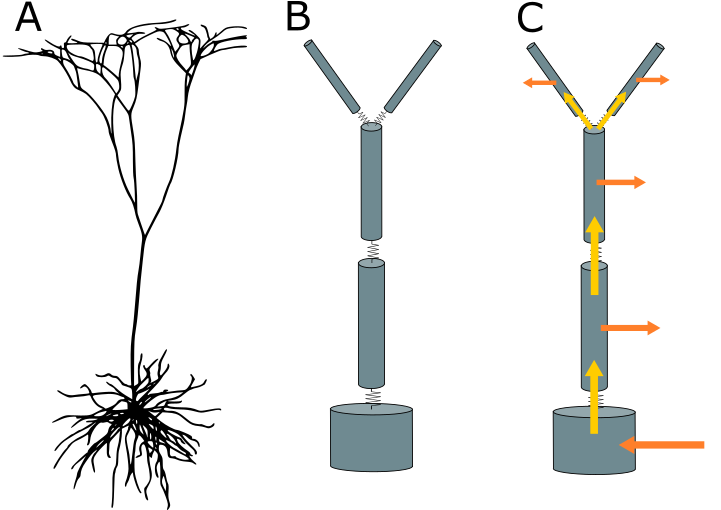
\includegraphics[width=0.6\textwidth]{Figures/Neuron/multicompartment.png}
\end{center}
\caption{\textbf{Multicompartmental modelling.}  (A) The neural morphology is (B) represented by a multicompartmental model, where the compartments are treated as cylinders connected by resistors. The example shows a crudely simplified model containing only five compartments, but detailed multicompartment models may include several hundreds of compartments, and can represent t he morphology in great detail. (C) Electric currents in the model can be separated into two groups: (i) transmembrane current in a compartment (green arrows), and (ii) intracellular currents between compartments (yellow arrows). 
}
\label{fig:Neuron:multicomp}
\end{figure}

Below, we first present a framework for modeling the transmembrane currents in a single compartment in \fref{sec:Neuron:membranecurrents}, and then go on to show how a number of such compartments can be connected together to a MC model in \fref{sec:Neuron:morphology}. Together, those two sections provide a theoretical framework for modeling neurons that should be sufficient for most practical applications. Readers that crave further biophysical insight into the ionic movements that mediate the transmembrane neural currents can get a brief introduction to this in \fref{sec:Neuron:Ions_and_reversals}. Finally, we end the chapter about neuronal modeling by briefly summarizing the main assumptions underlying the MC framework (\Fref{sec:Neuron:HHCassumptions}).


\section{\blue{Membrane currents}}
\label{sec:Neuron:membranecurrents}
\index{Hodgkin-Huxley type model}
Hodgkin-Huxley (HH) type models are called so because they describe the membrane mechanisms with a mathematical formalism similar to that used in celebrated model by \citeasnoun**{Hodgkin1952}. In HH-type models, the membrane typically includes three autonomous classes of transmembrane currents, normally represented as current densities (units \si{\milli\ampere\per\square\centi\metre}). These are (i) a capacitive current density ($i_{\mathrm{cap}}$), (ii) a the leakage current density ($i_{\mathrm{L}}$), and (iii) a the current density through active ion channels ($i_x$), of which there may be several different kinds ($x$ is an index). In addition, a neuron may receive (iv) external stimuli ($i_{\mathrm{stim}}$) either through synaptic currents or experimental current injections. 
\ehnote{Bedre symbol er $i_{\mathrm{ext}}$ for stroembidrag fra baade elektroder, synapser etc.}

In the case where the neuron is modeled as a single compartment, the transmembrane currents into that compartment must sum to zero, so that:
\begin{equation}
i_{\mathrm{cap}}+ i_{\mathrm{L}} + \sum_x{i_x} +  i_{\mathrm{stim}} = 0.
\label{eq:Neuron:singlecomp_zerosum}
\end{equation}
Below, we define the various currents that go into this equation.

\subsection{\blue{Capacitive current}}
\label{sec:Neuron:Cap}
\index{Capacitive current}
The capacitive current density,
\begin{equation}
i_{\mathrm{cap}}= c_{\mathrm{m}} \frac{dV}{dt},
\label{eq:Neuron:HHcap}
\end{equation}
represents the charging up of the membrane potential $V$ due to a charge density accumulating on the outside and inside of the capacitive membrane. 
\ehnote{I mine oerer skjaerer "charging up" noe. Kan vi ikke skrive "... represents the accumulation of charge in- and outside of the capacitive membrane as function of change in membrane potential $V$ over time."?}
Here, $c_{\mathrm{m}}$ is the \textit{specific membrane capacitance} defined as capacitance per membrane area. In the original HH model, $c_{\mathrm{m}}$ had the value 1 \si{\micro \farad / \cm}$^2$, and this value seems to be representative for most neurons.  An illustration of how to interpret the capacitive current is given in \fref{fig:Neuron:capacitive_currents}. 

\begin{figure}[!ht]
\begin{center}
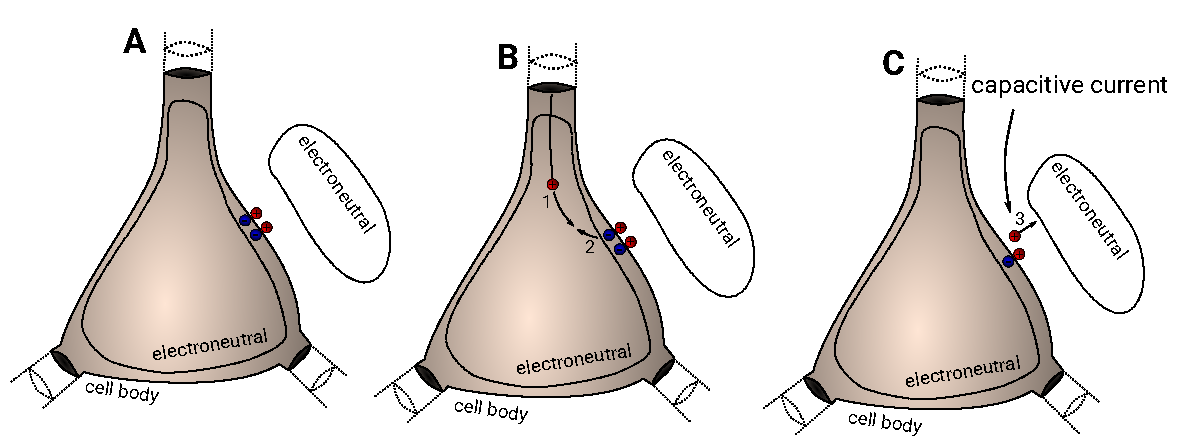
\includegraphics[width=1.0\textwidth]{Figures/Neuron/capacitive_currents.pdf}
\end{center}
\caption{\textbf{Capacitive currents are important for current \ehnote{"charge conservation" er et mer fundamentalt begrep} conservation.}  (\textbf{(A)}) The extracellular and intracellular bulk solutions are essentially electroneutral, and the only region where there is a nonzero charge density is in thin Debye layers around the capacitive membrane. Unlike the other currents involved, the capacitive current is not due to ions crossing the membrane, but due to ions piling up on either side of it, separating a membrane charge density $\eta$ and a charge membrane charge density $-\eta$, giving rise to a membrane potential of $V = \eta/c_{\mathrm{m}}$. An outward capacitive current could correspond to an anion leaving the membrane on the inside (\textbf{(B)}), which will coincide with a cation leaving the membrane on the outside (\textbf{(C)}). Thus, capacitive membrane currents do give rise to electrical ionic volume currents both in the intra- and extracellular space.
}
\label{fig:Neuron:capacitive_currents}
\end{figure}

If we insert \fref{eq:Neuron:HHcap} into \fref{eq:Neuron:singlecomp_zerosum}, we get:
\begin{equation}
c_{\mathrm{m}} \frac{dV}{dt} = - (i_{\mathrm{L}} + \sum_x{i_x} +  i_{\mathrm{stim}}),
\label{eq:Neuron:singlecomp_capinserted}
\end{equation}
which gives us an intuitive understanding of neurodynamics: If the sum of ionic currents over the membrane (right hand side) is nonzero, it will lead to a charging up (left hand side) of the membrane. \tvntxt{In other words, if for example positive ions are crossing the membrane and entering the cell (ionic current), this positive current will be exactly balanced by positive ions leaving the outside of the membrane because the cell has become less negative (capacitive current).}


\subsection{\blue{Leakage current}}
\label{sec:Neuron:leak}
\index{Leakage current}
The leakage current density is given by
\begin{equation}
i_{\mathrm{L}} = \bar{g}_{\mathrm{L}} (V - E_{\mathrm{L}}),
\label{eq:Neuron:HHleak}
\end{equation}
where $\bar{g}_{\mathrm{L}}$ (mS/cm$^2$) is the leak conductance (the bar indicates that it's a constant). 
\ehnote{Trengs virkelig den overline notasjonen? Lite konsekvent med andre parametre som ogsaa kun er skalarverdier. Veit det er brukt i HH-52-artikkelen, men virker litt utypisk i matte/fysikk ellers\ldots}
The factor $(V - E_{\mathrm{L}})$ (\si{\milli\volt}) is often called the driving force, and $E_{\mathrm{L}}$ the leak reversal potential\index{Reversal potential}. The biophysical origin of the reversal potential is explained later (see \fref{sec:Neuron:Ions_and_reversals}). For now, we may simply think of $E_{\mathrm{L}}$ as the "target potential" that the leakage current will strive to drive the membrane potential towards. In reality, the leakage current is not a single current, but represents an orchestra of physiological processes that together will drive the membrane potential towards the value $E_{\mathrm{L}}$. 

Together, the capacitive current and the leakage current determine the passive properties of the membrane. If the neuron were to include only these two currents, it could be well modeled as an RC-circuit, and RC-neuron\index{RC-neuron} models are often used to simulate the subthreshold dynamics of neurons (\Fref{fig:Neuron:RC}). 

\begin{figure}[!ht]
\begin{center}
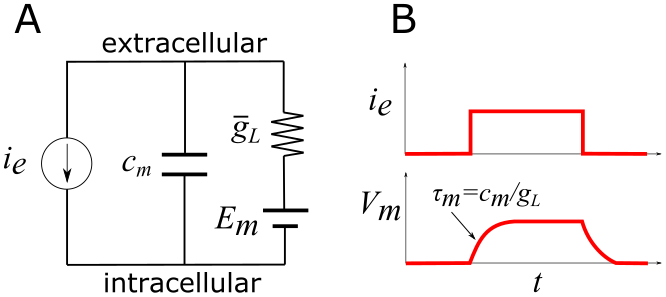
\includegraphics[width=0.8\textwidth]{Figures/Neuron/RCneuron.png}
\end{center}
\caption{\textbf{RC-neuron.}  A neuron model containing only a capacitive and a leakage current can be represented as an RC-circuit. To use standard MC modeling convention, we have expressed the various variables and parameters in units per membrane area: With a total membrane resistance $R = 1/(g_{\mathrm{L}} A)$, and capacitance $C = c_{\mathrm{m}}A$, we get that $RC = c_{\mathrm{m}}/g_{\mathrm{L}}$. In the illustration, the neuron is given an (electrode) injection $i_{\mathrm{e}}$ (A/cm$^2$) and responds by charging up the membrane. When the input is terminated, the membrane potential will return to the value $E_{\mathrm{L}}$. In the RC-model, $E_{\mathrm{L}}$ will be identical to the resting potential of the neuron, i.e., the potential that the membrane will settle on in the case where it does not receive any input. In models which include additional, active ion channels, these can in principle affect the resting potential, so that it may generally differ from $E_{\mathrm{L}}$.
}
\label{fig:Neuron:RC}
\end{figure}


\subsection{\blue{Active ion channels}}
\label{sec:Neuron:active}
\index{Ion channels! Voltage gated}
In addition to $i_{\mathrm{cap}}$ and $i_{\mathrm{L}}$, biophysical neuronal models include a number of active ion channels. These account for the fancy aspects of neurodynamics, 
\ehnote{"fancy" er vel kanskje litt upresist\ldots}
and the main legacy of Hodgkin and Huxley was that they derived a mathematical model for describing the kinetics of these \cite**{Hodgkin1952}.

In the HH-type formalism, the current through an active ion channel type $x$ is modeled as:
\begin{equation}
i_x = \bar{g}_x m_x^{\alpha} h_x^{\beta}(V-E_x).
\label{eq:Neuron:HHform}
\end{equation}
We note that the current density $i_x$ does not represent the current through a single ion channel, but a large number of channels of the same type $x$. Thus, $\bar{g}_x$ (\si{\milli\siemens\per\square\centi\metre}) denotes the conductance when all channels of type $x$ are fully open (the bar indicates that it's a constant),
\tvnnote{Jeg ble fortalt en gang at dette ikke noedvendigvis var sant, og at parameterne kunne vaere slik at $m$ og $h$ aldri kunne naa 1, men husker ikke helt hva dette handlet om.}
\ehnote{Sannsynlighet for aapning/lukking som disse variablene representerer er kun paa intervallet $\langle 0, 1 \rangle$}
 while $E_x$ (\si{\milli\volt}) is the reversal potential for the ion species that travels through the channel type. In analogy with the leak reversal potential, we may think of $E_x$ as the target potential that the current through ion channel $x$ will strive to drive the membrane potential towards. The intrinsic membrane potential dynamics is thus due to the competition between various currents that all try to drive it towards their respective reversal potentials. 

If one prefers to think of neurons in terms of circuit diagrams, the active ion channels are simply added in parallel to the passive $i_{\mathrm{cap}}$ and $i_{\mathrm{L}}$ currents. As an example, the electric circuit representation of the HH model is depicted in \Fref{fig:Neuron:HH}.

\begin{figure}[!ht]
\begin{center}
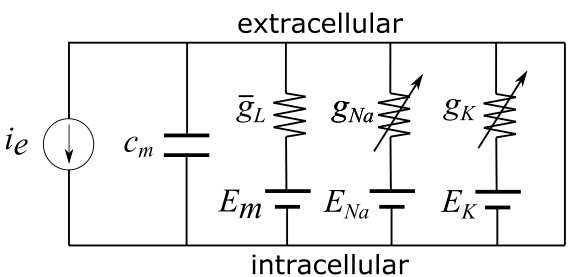
\includegraphics[width=0.8\textwidth]{Figures/Neuron/HHmodel.png}
\end{center}
\caption[]{\textbf{Active, single compartment neuron model.}  In addition to a capacitive and a leakage current, active neuron models contain a number of active ion channels. The example diagram shows the original Hodgkin-Huxley model, with an active Na$^+$ and an active K$^+$ channel. The arrows slicing the diagram conductances indicate that they are variables.}
\label{fig:Neuron:HH}
\end{figure}

Active ion channels differ from the passive leakage channel in that their total conductance, $\bar{g}_{x} m^{\alpha} h^{\beta}$, vary with time due to the so-called gating variables, in \fref{eq:Neuron:HHform} denoted $m$ and $h$\index{Gating variables}. These determine how the ion channels activate or deactivate (open or close), and $m$ and $h$ represent two different types of gates differing in terms of their opening/closing dynamics. The exponents $\alpha$ and $\beta$ represent the number of copies that a channel $x$ has of each type of gate. At the level of a single ion channel the values of $m$ and $h$ would interpret as the \textit{probability} that a given gate is in the open state. However, when we deal with summed currents through a large number of ion channels, the values of $m$ and $h$ interpret as the \textit{fraction} of the gates of the various types that are open. The values are thus numbers between 0 (all gates in the closed state) and 1 (all gates in the open state). The product $m^{\alpha} h^{\beta}$ thus interprets as the fractions of ion channels in which all gates are open so that currents can pass through. The ion channel conductance is thus given by the product $\bar{g}_x m_x^{\alpha} h_x^{\beta}$.

For voltage-gated ion channels, the the dynamics of the gating variables can be described by kinetics equations on the form:
\begin{equation}
\frac{dx(V,t)}{dt} = \frac{x_{\infty}(V) - x}{\tau_x(V)},  \, \text{for } x = \{m,h\}.
\label{eq:Neuron:HHgate}
\end{equation}
\ehnote{$x \in \{m, h\}$ siden $x$ er et diskret element i settet.}
Here, the steady state activation $x_{\infty}(V)$, represents the fraction of gates that will end up in the open state if the cell is clamped at a given potential $V$ for sufficiently long time. However, the process of opening the gates takes some time, as accounted for by the activation time constant $\tau_x(V)$ (\si{\milli\second}). Both $x_{\infty}(V)$ and $\tau_x(V)$ are functions of the membrane potential, and these must be determined experimentally for each individual ion channel type. We do not go into the experimental challenges here, but will think of them as known functions. 

There are also many ion channels whose activation or inactivation do not depend on $V$, but on some other variable, such as the concentration of some ion species or ligand \cite**{Hille2001,Sterratt2011}. A common example are Ca$^{2+}$ gated ion channels, i.e., channels with gate opening controlled by the intracellular Ca$^{2+}$ concentration ($\mathrm{[Ca^{2+}]_i}$). There are also ion channels whose activation depend on more than one variable, such as e.g., ion channels whose activation depend on both $V$ and $\mathrm{[Ca^{2+}]_i}$. A HH-type formalism can in most cases be applied also to these kind of ion channels, provided that $x_{\infty}(V)$ and $\tau_x(V)$ in \fref{eq:Neuron:HHgate} can be replaced with experimentally determined functions of the relevant variables \cite**{Sterratt2011}.

To give an example of an active neuron model, the full set of equations for the HH model is summarized in Box \ref{box:Neuron:HH}. Compared to modern biophysically detailed neuron models, the original HH model is relatively simple in that it only contains two (voltage-gated) active ion channels, a Na$^+$ with three activation gates ($m^3$) and one inactivation gate ($h$), as well as a K$^+$ channel with four inactivation gates $n^4$. The two active ion channels are together responsible for action potential generation.  

\begin{floatingbox}[h]
\caption{Hodgkin-Huxley equations}

\begin{eqnarray*}
    c_{\mathrm{m}} \frac{dV}{dt} & =  & -\bar{g}_{\mathrm{L}}(V-E_{\mathrm{L}}) - \bar{g}_{\mathrm{Na}} m^3 h (V - E_{\mathrm{Na}}) - \bar{g}_{\mathrm{K}} n^4 (V - E_{\mathrm{K}}) \\
    \frac{dx(V,t)}{dt} & = & \frac{x_{\infty}(V) - x}{\tau_x(V)},  \, \text{for } x = \{m,h,n\} \\ 
    x_{\infty}(V) &= & \frac{\alpha_x(V)}{\alpha_x(V) + \beta_x(V)}, \, \text{for } x = m,n,h \\ %\hline
    \tau_x(V) & = & \frac{1}{\alpha_x(V) + \beta_x(V)}, \, \text{for } x = m,n,h \\ %\hline
    \alpha_n &=& \frac{0.01 \mathrm{ms}^{-1} V+55\,\si{\milli\volt}}{1-e^{-(V+55\,\si{\milli\volt})/10\,\si{\milli\volt}}}  \\ %\hline
     \beta_n &=& 0.125 \mathrm{ms}^-1 e^{-(V+65\,\si{\milli\volt})/80\,\si{\milli\volt}}   \\ %\hline
     \alpha_m &=& \frac{0.1 \mathrm{ms}^{-1} V+ 40\,\si{\milli\volt}} {1-e^{-(V+40\,\si{\milli\volt})/10\,\si{\milli\volt}}}  \\   
     \beta_m &=& 4 \mathrm{ms}^{-1} e^{-(V+65\,\si{\milli\volt})/18\,\si{\milli\volt}}  \\ %\hline
    \alpha_h &=& 0.07 \mathrm{ms}^{-1} e^{-(V+65\,\si{\milli\volt})/20\,\si{\milli\volt}}  \\ %\hline
    \beta_h &=& \frac{1 \mathrm{ms}^{-1}}{1+e^{-(V+35\,\si{\milli\volt}))/10\,\si{\milli\volt})}}   \\ %\hline
    c_\mathrm{m} &=& 1.0 \,\si{\micro\farad\per\square\centi\metre} \\ %\hline
    \bar{g}_{\mathrm{Na}} &=& 120 \,\si{\milli\siemens\per\square\centi\metre}\\ %\hline
    \bar{g}_{\mathrm{K}} &=& 36 \,\si{\milli\siemens\per\square\centi\metre} \\ %\hline
    \bar{g}_{\mathrm{L}} &=& 0.3 \,\si{\milli\siemens\per\square\centi\metre} \\ %\hline
    E_{\mathrm{Na}} &=& 50 \,\si{\milli\volt} \\ %\hline
    E_{\mathrm{K}} &=& -77  \,\si{\milli\volt} \\ %\hline
    E_{\mathrm{L}} &=& -54.4 \,\si{\milli\volt} \\ %\hline
\end{eqnarray*}
\label{box:Neuron:HH}
\end{floatingbox}


\ehnote{Burde ikke andre formalismer som termodynamiske og stokastiske (Markov?) modeller nevnes? HH formalismen er vel kun en empirisk approksimasjon som ikke ivaretar fundamentale fysiske prinsipp (energibevaring for eksempel).}



\subsection{\blue{Stimulus currents and synapses}}
\label{sec:Neuron:stim}
\index{Stimulus currents}
The stimulus current in \fref{eq:Neuron:singlecomp_zerosum} can represent any external stimulus that a neuron receives. Typically, it is either taken to represent an experimental electrode injection or a synaptic input. Below we include some typical examples of stimuli used in neuron simulations. 

\subsubsection{Current injections}
An electrode injection such as a step-current injection is modeled as:
\begin{equation}
i_\text{e}(t)= 
\begin{cases}
    constant, & \text{if } t_{start} < t < t_{end} \\
    0,              & \text{otherwise},
\end{cases}
\label{eq:Neuron:injected}
\end{equation}
\ehnote{$\text{for } t \in [t_\mathrm{start}, t_\mathrm{end}]$ - en annen ting er vel at oftest representeres disse punkt-stroemmene med enhet ampere, saa symbol $I_\mathrm{e}$}
Of course, one may chose the stimulus to be any function of time.


\subsubsection{Conductance-based synapses}
\index{Synapse}
\label{sec:Ch-Neuron:conductance-based-synapses}
A chemical synapse can be modeled more or less like an ion channel:
\begin{equation}
i_\text{syn}(t) = {g}_\text{syn}(t) \big(V(t)-E_\text{syn} \big), 
\label{eq:Neuron:chemicalsynapse}
\end{equation}
where $g_\text{syn}(t)$ is the synaptic conductance and $E_\text{syn}$ is the reversal potential of the synapse. 
\ehnote{jeg er litt forvirra, er synaptic conductance per areal eller ikke? Enhet S vs. S~m$^{-2}$? Jeg tenker synapser er punktprosesser uten romlig utstrekning saa enhet S og derfor notasjon $I_\mathrm{syn}, G_\mathrm{syn}$ Schuetter bruker liten bokstav av en eller annen grunn.}

The value of $E_\text{syn}$ determines whether the synapse is \textit{excitatory}, which means that it will tend to drive the  membrane potential of neuron toward the threshold for generating action potentials, or \textit{inhibitory}, which means that it will tend to drive the neuron away from the threshold for generating action potentials. Examples of excitatory synapses are AMPA and NMDA synapses, in which $E_\text{syn}$ ($\sim$ 0 - 10 mV) is high above the neuronal resting potential. The most common inhibitory synapse is the GABA synapse, in which $E_\text{syn}$ ($\sim$ - 70 mV) is close to the resting membrane potential of the neuron.

The synapse model described by \fref{eq:Neuron:chemicalsynapse} is called \textit{conductance based}, because the activation of the synapse is modeled as a transient change in the synaptic conductance. Unlike for ion channels, which are often voltage or calcium activated, the chemical synapse is activated by neurotransmitters received from a pre-synaptic cell. However, the synaptic response tends to be rather stereotypical, meaning that the post-synaptic conductance change is more or less the same every time the synapse is activated \tvnnote{Har vi kilde paa dette? Er dette egentlig sant? Har jo STD, STP osv. Swadlow 2002 for eksempel finner jo ganske andre resultater}. 
It is therefore not common to model neurotransmitter activation explicitly, but instead just
model $g_\text{syn}(t)$ as a constant $\bar{g}_\text{syn}$ multiplied with a temporal kernel determining the opening and closing of a synapse set off at an activation time $t_s$:
\begin{equation}
i_\text{syn}(t) = \bar{g}_\text{syn} f(t) \big(V(t)-E_\text{syn} \big).
\label{eq:Neuron:chemicalsynapse}
\end{equation}
Typical choices for $f(t)$ are\index{Synapse models}: 
\begin{align}
&\text{(i) exponential decay:} \;\; f(t) = e^{-(t-t_\text{s})/\tau}\, \Theta(t-t_\text{s}) \\
&\text{(ii) $\alpha$-function:} \;\; f(t) =  \frac{t-t_\text{s}}{\tau} e^{-(t-t_\text{s})/\tau} \, \Theta(t-t_\text{s}) \\
&\text{(iii) $\beta$-function:} \;\; f(t) = \frac{\tau_1 \tau_2}{\tau_1-\tau_2} 
\Big( e^{-(t-t_\text{s})/\tau_1} - e^{-(t-t_\text{s})/\tau_2} \Big) \, \Theta(t-t_\text{s}) \\
& \text{(iv) NMDA-like:} \;\; f(t) = \frac{e^{-(t-t_\text{s})/\tau_1} - e^{-(t-t_\text{s})/\tau_2}} {1+\mu [\text{Mg}^{2+}] e^{-\gamma V} } \, \Theta(t-t_\text{s}),
\label{eq:Neuron:sf4}
\end{align}
where $\Theta(t)$ is the (Heaviside) unit step function: $\Theta(t \ge 0)=1$,  $\Theta(t< 0)=0$, and where parameters like $\gamma$,  $\tau$, $\tau_1$ and $\tau_2$ must be tuned to experimental data from the particular synapse type that one wants to model. Simple waveform (cf., (i)--(iii) above) typically used for AMPA  and GABA synapses, while the waveform (iv), is mainly relevant for NMDA-synapses, where the conductance is influenced by membrane voltage and concentration of extracellular magnesium. 

The strength or efficacy of synaptic transmission may change over time through various processes that are often grouped together under the term "synaptic plasticity". Synaptic plasticity work as a mechanism for learning and memory formation in the brain. It is a much studied topic that has been treated in several text books (see e.g., \citeasnoun**{Joel1993} or \citeasnoun**{Kreutz2012}). We will not go further into this topic here.


\subsubsection{Current-based synapses}
\label{sec:Ch-Neuron:current-based-syn}
Currents through conductance-based synapses depend on the driving force, $V(t)-E_\text{syn}$ (\fref{eq:Neuron:chemicalsynapse}). A simpler synapse model is the current-based synapse, which rests on the assumption that the driving force $V(t)-E_\text{syn}$ can be approximated by a constant. The synaptic current then becomes:
\begin{equation}
i_\mathrm{syn}(t) = \overline{i}_\mathrm{syn} f(t), 
\label{eq:Neuron:CurrentBasedSynapse}
\end{equation}
where (cf. \fref{eq:Neuron:chemicalsynapse}):
\begin{equation}
\bar{i}_\mathrm{syn}=\bar{g}_\mathrm{syn}(\langle V(t) \rangle_t -E_\mathrm{syn}),
\label{eq:Neuron:CurrentBasedAvg}
\end{equation}
and where $\langle V(t) \rangle_t$ denotes the temporal average of the membrane potential. The temporal kernel
$f(t)$ can have the same exponential waveforms (i)-(iv) as the conductance based synapses. 
\ehnote{Jeg tenker subfix $t$ kan droppes siden $V(t)$ er 1D}

Unlike conductance-based synapses, current-based synapses are independent of the state ($V(t)$) of the neuron, and synaptic events thus become independent of previous synaptic events, something that facilitates the derivation of analytical solutions \cite**{Richardson2004,Cavallari2014}. Their relative simplicity have made current-based synapses popular in large network simulations because they reduce the computational load. 
\tvnnote{Should mention that they are linear}
\ehnote{Jeg tenker det er mer til det enn dette - for NEURON sin del er det lite aa hente paa lineariserte synapser siden MC formalismen krever numerisk integrasjon uansett - for punktnevroner med linear subthreshold dynamics (LIF etc.) kan man bruke eksakt integrasjon som er kjapt (i NEST for eksempel).}

\ghnote{Jeg skrev ikke mer enn det som staar over. Er det tilstrekkelig? Jeg ser at Espen har lagt inn noen kommentarer under, men trenger vi aa gaa inn paa disse tingene her? Espen, kan du se paa det, skrive inn noe ekstra om du mener det skal inn dit, og fjerne kommentarene hvis ikke?}

\ghnote{Man kunne jo skrevet flere sider om denne approksimasjonen, men jeg vet ikke hvor dypt vi vil gaa inn i dette.Jeg har ikke DeSchutter-boka, men har en hunch om at vi kan referere til den her. Er lite erfaren med bruk av slike synapser, og vet ikke hva de relevante referanser er. Espen - har du noe du vil legge til?}
\ehnote{Tok bort referansen til Hagen2016. Vi utleda ingen "closed-form solutions" der for dette. Vaart valg av synapsemodell var hentet direkte fra synapsemodellen i Potjans\&Diesmann2014. LIF punkt-nevroner med stroembaserte synapser kan loeses eksakt uten numerisk integrasjon og er populaert i kontekst av NEST for eksempel. Naa har vel andre studier som Roessert2016 (https://arxiv.org/abs/1604.00087) for eksempel vist at man kan approksimere effekten av dendrittisk kabel og synapsetroem med et ekvivalent filter, som implisitt resulter i en stroembasert "synapse" saa vidt jeg husker.}

\subsubsection{Gap-junctions}
\tvnnote{Brukes dette senere i boka? Hvis ikke kan vi kanskje ta det bort for enkelhets-skyld?}
\ehnote{Jeg ville beholdt dette - gap junctions er "vanlige". Om vi bruker de er en annen ting ;)}
In addition to the chemical synapses, some neurons also form electrical synapses called \underline{gap junctions}. A gap junction is basically an electric coupling between a branch of one neuron (with membrane potential $V_1$) and a branch of another neuron (with membrane potential $V_2$). The current through the gap junction is then simply the synaptic conductance multiplied with the voltage difference between the coupled branches:

\begin{equation}
i_\text{gap}=g_\text{gap} (V_{\mathrm{m}2}-V_{\mathrm{m}1}).
\label{eq:Neuron:gapjunction}
\end{equation}



%%%%%%%%%%%%%%%%%%%%%%%%%%
\section{\blue{Morphology}}
\label{sec:Neuron:morphology}
\index{Multicompartmental neuron model}
When we above introduced the various membrane currents, we mostly pictured the neuron as being a single compartment. In doing that, we implicitly assumed that the whole neuron was isopotential (same $V$ everywhere). 
\ehnote{Ikke aner jeg hvorfor det refereres til at antagelsen er 'isopotential compartments' - spesielt siden dette ville resultert i null aksialstroem og null transmembran stroem. For vaart formaal er vel en antagelse om tilnaermet konstant transmembran stroemtetthet langsmed hvert compartment langt bedre! Se foeroevrig kap 4.1.2 og kap 5.2.4.1 i NEURON-boka, potensialet til et kompartment er kun gyldig midt paa.}
However, in neurons with long and branchy dendrites, $V$ in the soma can be completely different from $V$ in the tip of a distal dendrite. If we want to account for the spatial aspect of neuronal signaling, we need to use multicompartmental (MC) models, where the neural morphology is represented as cylindrical compartments connected with resistors, and $V$ can be computed in each individual compartment (\Fref{fig:Neuron:multikompisen}A). 

\begin{figure}[!ht]
\begin{center}
\includegraphics[width=0.7\textwidth]{Figures/Neuron/multikompis.png}
\end{center}
\caption{\textbf{Multi-compartment model.} {\bf (A)} Representations of a neuronal morphology as a number of interconnected compartments. {\bf (B)} Subset of interconnected compartments. The currents involved in MC modeling include the sum of transmembrane currents ($I_{\mathrm{m},n}$) in a compartment $n$, and the intracellular currents running between 
compartments, $I_{n-1,n}$ (current from compartment $n-1$ to $n$), and $I_{n,n+1}$ (current from compartment $n$ to $n+1$).
}
\label{fig:Neuron:multikompisen}
\end{figure}

As a simple introduction to the formalism used in MC models, let us consider a subset of three connected cylindrical compartments which we number $n-1$, $n$ and $n+1$ (\Fref{fig:Neuron:multikompisen}B). For simplicity, we assume that the three cylinders have the same length ($L$) and diameter ($d$). The two categories of currents that run in this system are (i) the transmembrane currents that we introduced in the previous subsection, all of which we for now can group together into a total transmembrane current $I_{\mathrm{m},n}$, and (ii) the axial currents running between the cylindrical compartments ($I_{n-1,n}$ and $I_{n,n+1}$). The dynamics of this system is computed using Kirchhoff's current law, which demands that the sum of currents into a given compartment ($n$) should be zero:
\begin{equation}
I_{n-1,n} - I_{n,n+1} - I_{\mathrm{m},n} = 0.
\label{eq:Neuron:Kirch}
\end{equation}
We note that we here work with total currents (units \si{\ampere}), not current densities, so that $I_{\mathrm{m},n}$ is the sum of all current densities in the left hand side of \fref{eq:Neuron:singlecomp_zerosum} multiplied with the membrane area of compartment $n$. 

The axial current between two compartments is proportional to the voltage difference between the compartments, as determined by Ohm's law:
\begin{eqnarray}
I_{n-1,n} = \frac{V_{n-1}-V_n}{4 R_\text{a} L/(\pi d^2)}, \nonumber \\ 
I_{n,n+1} = \frac{V_{n}-V_{n+1}}{4 R_\text{a} L/(\pi d^2)}.
\label{eq:Neuron:axialcurrents}
\end{eqnarray}
Here, the denominators represent the axial resistance between two compartments, defined in terms of the axial resistivity $R_\text{a}$ (\si{\ohm\centi\metre}), a material property of the cytosol solution, the cross-section area, $\pi d^2/4$, and the segment length or travel distance, $L$ (\si{\metre})\tvnnote{Er L i meter?}. 

The calculations become more complicated when the connected cylinders are of different length and diameter, and especially at branch points. However, the theory for computing the dynamics in branching structures with varying diameters is well established \cite**{Rall1977,Rall1989}, and designated software such as NEURON \cite**{Hines1997,Hines2009} automatizes the compartmentalization for the user once the neural morphology is specified. For the reminder of this chapter, we limit ourselves to consider the simplified, unbranched scenario (\Fref{fig:Neuron:multikompisen}B), as we deem this as sufficient for establishing an understanding of the essentials of morphology\tvnnote{MC?} modeling. 

We note that in \fref{eq:Neuron:axialcurrents}, $V_n$ is the \emph{intracellular} potential in compartment $n$. However, in MC models, the intracellular potential is assumed to be identical to the membrane potential. This amounts to assuming that the extracellular resistivity is zero, so that the extracellular space is isopotential and grounded ($V = 0$ there) \tvnnote{Kan kanskje si: This amounts to assuming that any changes in the extracellular potential along the cell are small enough to have a negligible effect on the neural activity.}. This may seem like a peculiar assumption to make in a book where the extracellular potential is the main topic. We comment further on this assumption and its consequences at the end of this chapter. For now, we simply note that although the extracellular potential in reality is not zero, it is generally so much smaller than the intracellular potential that we can assume that it is zero without going too wrong when computing the neurodynamics. 


%%%%%%%%%%%%
\subsection{\blue{Active multicompartment models}}
\label{sec:Neuron:Active_multicomp}
To specify our MC neuron model further, we write out the total membrane current as:
\begin{equation}
I_{\mathrm{m},n} = I_{\mathrm{cap},n} + I_{\mathrm{ion},n} + I_{\mathrm{stim},n} = -\pi d L c_\text{m} \frac{dV_n}{dt} + \pi d L i_{\mathrm{ion},n} + I_{\mathrm{stim},n}
\label{eq:Neuron:Imemb}
\end{equation}
where $I_{\mathrm{ion},n}$ represents the total transmembrane ionic currents through leakage and active ion channels. In the last step, we expressed the capacitive and ionic currents (\si{\milli\ampere}) as current densities (\si{\milli\ampere\per\square\centi\metre}) multiplied with the membrane area ($\pi d L$ (\si{\square\centi\metre})) represented by the sides of the cylinder, and we have inserted \fref{eq:Neuron:HHcap} for the capacitive current density. If we insert this into \fref{eq:Neuron:Kirch}, we get the fundamental equation for multicompartmental models:

\begin{equation}
c_\text{m} \frac{dV_n}{dt} = i_{\mathrm{ion},n} + \frac{d}{4R_\text{a}}\left(\frac{V_{n+1}-V_n}{L^2} - \frac{V_n-V_{n-1}}{L^2} \right) + \frac{i_{\mathrm{stim},n}}{\pi d L}.
\label{eq:Neuron:multimain}
\end{equation}
\Fref{eq:Neuron:multimain} assumes that a compartment $n$ has two neighbors ($n-1$ and $n+1$), which will not be true for the endpoint compartments. To solve it, we must therefore select appropriate boundary conditions for these compartments. Common boundary conditions are those of a sealed end, where $\frac{\partial V_n}{\partial x} = 0$ for $n$ at the endpoints, or a killed end, where $V_n=0$ for $n$ at the endpoints. The NEURON simulator by default uses the sealed-end condition, which means that no axial current leaves at the endpoints of the simulated structure. 


%%%%%%%%%%%%%%%%%
\subsection{\blue{Passive multicompartment models}}
\label{sec:Neuron:Passive_multicomp}
\index{Multicompartmental neuron model}
If the neuron contains no active ion channels, $i_{\mathrm{ion},n} = g_\text{L}(V_n - E_L)$ is simply the leakage current density, and $E_L$ becomes identical to the membrane resting potential. It is then common to denote it by $E_\text{m}$, and to replace the leak conductance $g_\text{L}$ with the membrane resistivity $R_\text{m} = 1/g_\text{L}$ (\si{\ohm\square\centi\metre}). \Fref{eq:Neuron:multimain} then simplifies to:

\begin{equation}
c_\text{m} \frac{dV_n}{dt} = \frac{E_\text{m}-V_n}{R_\text{m}} + \frac{d}{4R_\text{a}}\left(\frac{V_{n+1}-V_n}{L^2} - \frac{V_n-V_{n-1}}{L^2} \right) + \frac{I_\text{stim}}{\pi d L}
\label{eq:Neuron:multipassive}
\end{equation}
\tvnnote{Stor I?}
\ehnote{ser riktig ut her, men ikke over i likning 3.20}.
Although all neurons contain some active membrane mechanisms, the passive model (\fref{eq:Neuron:multipassive}) is often used as an approximation for signaling in neural dendrites, which tend to have a lower density of active mechanisms compared to the soma and axon. 
\tvnnote{paapeke at nevroner ofte er nesten passive litt unna threshold? (eksempel i Figure 9.5))}

An illustration of passive signal propagation is shown in \fref{fig:Neuron:Semiinf}A, which shows the membrane potentials at selected positions along a 1000~\si{\micro\metre} long stick-neuron responding to a stimulus resembling a synaptic input in one end. We see that the peak response comes faster in proximal than in distal locations, and that the peak response decays with distance from the synapse. We also see that potential at all points along the stick become level a few milliseconds after the stimulus was delivered, after which $V$ decays gradually towards the resting potential. These simulations on a passive model give a qualitative idea on how signals spread in dendrites. As we shall see below, the passive model is also useful in that it allows us to derive some analytical results for signal propagation in neural branches.

\begin{figure}[!ht]
\begin{center}
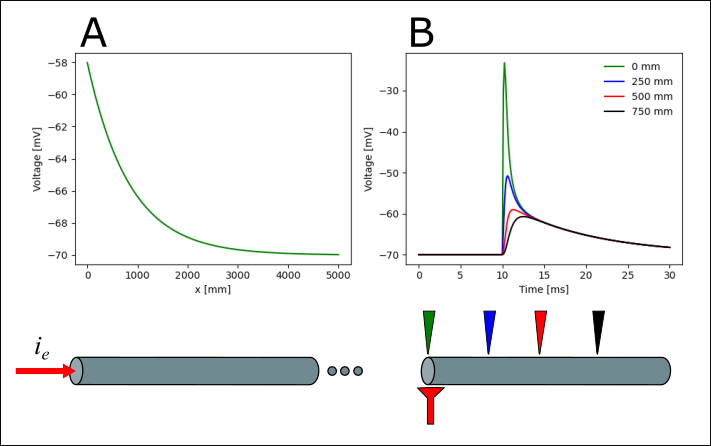
\includegraphics[width=0.7\textwidth]{Figures/Neuron/Cablesims.png}
\end{center}
\caption{\textbf{Stick-neuron responding to transient and constant inputs received in one end.} (A) Finite cable of length $L = 1 \, \si{\milli\metre}$ simulated numerically as 100 compartments, and stimulated with an alpha-synapse in the first compartment ($0<x<10 \, \si{\micro\metre}$). Transient responses shown at different distances from the synapse. The peak response decreases with distance from the synapse, and the time to reach the peak increases with distance from the synapse.
(A) Analytical steady-state solution for semi-infinite cable receiving a constant input $I_\text{stim} = 0.1 \, \si{\nano\ampere}$ in a sealed end at $x=0$. The membrane potential decays exponentially with distance from the stimulus site.  (A-B) Parameters choices: $c_\text{m}=1\, \si{\micro\farad\per\square\centi\metre}$, $d = 1\, \si{\micro\metre}$, $R_\text{a}=35.4\, \si{\ohm\centi\metre}$, $R_\text{m} = 10 \, \si{\kilo\ohm\square\centi\metre}$, which gives a length constant $\lambda = 840\, \si{\micro\metre}$.}
\label{fig:Neuron:Semiinf}
\end{figure}


%%%%%%%%%%%%%%%%%%%%
\subsection{\blue{Cable equation}}
\label{sec:Neuron:cableeq}
\index{Cable equation}
If we in \fref{eq:Neuron:multipassive} let $L \rightarrow \delta x$, and take the limit $\delta x \rightarrow 0$, we can derive the cable equation (see e.g., \cite**{Sterratt2011}): 

\begin{equation}
c_\text{m} \frac{\partial V}{\partial t} = \frac{E_\text{m}-V}{R_\text{m}} +  \frac{d}{4 R_\text{a}}  \frac{\partial^2 V}{\partial x^2}  + \frac{\mathcal{I}_{\mathrm{stim}}}{\pi d},
\label{eq:Neuron:cable}
\end{equation}
where we have introduced the stimulus current per unit length,
\ehnote{synes det er mindre kloenete aa definere denne som $I_\mathrm{stim}(x, t)$ i enhet A direkte. $\mathcal{I}_\mathrm{stim}(x,t)$ dukker jo bare opp en gang nedenfor for saa aa bli omdefinert til $I_\mathrm{stim}(x,t)$ igjen.} 
\begin{equation}
\mathcal{I}_{\mathrm{stim}}(x,t) = \lim_{\delta x \to 0} I_{\mathrm{stim}}(x,t)/\delta x \,\; (\si{\milli\ampere\per\centi\metre}). 
\label{eq:Neuron:CurrentPerUnitLength}
\end{equation}
To improve our analytical understanding of dendritic signaling, it is useful to reformulate the cable equation to:
\begin{equation}
\tau_\text{m} \frac{\partial V}{\partial t} = E_\text{m}-V +   \lambda^2  \frac{\partial^2 V}{\partial x^2}  + \frac{R_\text{m} \mathcal{I}_{\mathrm{stim}} }{\pi d},
\label{eq:Neuron:cable2}
\end{equation}
where we have multiplied all terms with $R_\text{m}$ and introduced the length constant \index{Length constant},
\begin{equation}
\lambda = \sqrt{\frac{d R_\text{m}}{4 R_\text{a}}} \,\; (\si{\centi\metre}), 
\label{eq:Neuron:lengthconst}
\end{equation}
and the time constant \index{Membrane time constant}, 
\begin{equation}
\tau_\text{m} \equiv R_\text{m} c_\text{m}  \,\; (\si{\milli\second}).
\label{eq:Neuron:timeconst}
\end{equation}
Here, $\tau_\text{m}$ is typical time scale (dimensionless time: $t/\tau$), while $\lambda$  is typical length scale  (dimensionless length: $x/\lambda$) for signals in the cable. If a certain point along the cable is perturbed, so that the potential is shifted from rest to a given value $V$, $\tau_\text{m}$ will determine how fast the local potential falls back towards rest, while $\lambda$ will tell us how far the local perturbation will spread along the cable. 

The cable equation is a continuous version of \fref{eq:Neuron:multipassive}. Whereas MC models generally must be solved numerically, the cable equation allows the spatiotemporal evolution of the membrane potential to be solved analytically for some idealized scenarios. Below, we consider a couple of scenarios that will  make the interpretation of $\tau_\text{m}$ and $\lambda$ clearer. 


%%%%%%%%%%%%%%%%%%%%
\subsection{\blue{Steady state solution of the cable equation}}
\label{sec:Neuron:cableSS}
\tvnnote{Bruker vi dette noe sted?}
Let us find the steady state solution for a semi-infinite cable, receiving a constant current injection at a sealed end in $x=0$ (\Fref{fig:Neuron:Semiinf}B). Since only the end-point receives the stimulus, we may attack this problem by solving \fref{eq:Neuron:cable2} for all other points $x>0$, and then introduce the stimulus current as a boundary condition. 

At steady-state, $\partial V/\partial t = 0$, and \fref{eq:Neuron:cable2} becomes:
\begin{equation}
0 = E_\text{m}-V +  \lambda^2 \frac{\partial^2 V}{\partial x^2}, 
\label{eq:Neuron:semiinf}
\end{equation}
at all points along the cable, except $x=0$. If we introduce the new variable $\Delta{V}=V-E_\text{m}$, \fref{eq:Neuron:semiinf} simplifies to:
\begin{equation}
\frac{d^2 \Delta{V}}{d x^2} -  \frac{1}{\lambda^2} \Delta{V}=0, 
\label{eq:Neuron:semiinf2}
\end{equation}
which has the solution:
\begin{equation}
\Delta{V}(x) = \Delta{V}(0) e^{-x/\lambda}, 
\label{eq:Neuron:semiinf3}
\end{equation}
or, 
\begin{equation}
V(x) = E_\text{m} + \big( V(0)-E_\text{m} \big) e^{-x/\lambda}.
\label{eq:Neuron:semiinf4}
\end{equation}
We note that the general-solution to \fref{eq:Neuron:semiinf2} also has a term containing $e^{+x/\lambda}$, but this was excluded on the count of being unphysical, since it diverges when $x \rightarrow \infty$. 

To obtain the final solution of the problem, we need to specify the boundary value $V(0)$, which will depend on the stimulus current. Since the stimulus is injected in a singular point ($x=0$), we go back to expressing in terms of a total current, $I_\text{stim}$ (and not as a current per unit length $\mathcal{I}_\text{stim}$). We can introduce it through a boundary condition demanding that the injected current must be identical to the axial current in the cable at $x=0$:
\begin{equation}
I_\text{stim} = - \frac{\pi d^2}{4}\frac{1}{R_\text{a}} \frac{\partial V}{\partial x}   \Big|_{x=0}.
\end{equation}
If we insert for $\partial V/\partial x$ (calculated from \fref{eq:Neuron:semiinf4}), and insert \fref{eq:Neuron:lengthconst} for $\lambda$, we can derive the following expression for $V(0)$:
\begin{equation}
V(0) = E_\text{m} + R_{\infty}I_\text{stim}, 
\label{eq:Neuron:firstRinf}
\end{equation}
where we have defined:
\begin{equation}
R_{\infty} = \sqrt{\frac{R_\text{m} R_\text{a}}{\pi^2 d^3}}.
\label{eq:Neuron:Rinf}
\end{equation}
If we now insert \fref{eq:Neuron:firstRinf} into \fref{eq:Neuron:semiinf3}, we obtain our final solution:
\begin{equation}
V(x) = E_\text{m} +R_{\infty}I_\text{stim}  e^{-x/\lambda}.
\label{eq:Neuron:semiinf4}
\end{equation}

The steady state solution to the semi-infinite cable (plotted in \Fref{fig:Neuron:Semiinf}B) is useful as it gives us analytical insight into signals spreading in e.g., passive dendrites. Some insights that can be derived from it is:

\begin{itemize}

\item It follows from \fref{eq:Neuron:firstRinf} that $R_{\infty} = (E_\text{m}-V(0))/I_\text{stim}$, and thus interprets as the steady-state input resistance of the semi-infinite cable. \Fref{eq:Neuron:Rinf} thus shows that the input resistance is proportional to $1/d^{3/2}$, i.e., the input resistance is higher the thinner the dendrite. 

\item \Fref{eq:Neuron:semiinf4} shows that in steady-state, the amplitude will decay exponentially from the injection site and outwards, and will be reduced by a factor $1/e$ over the length $\lambda$. If we insert some typical values into \fref{eq:Neuron:lengthconst}, like a dendritic diameter of $d=1 \, \si{\micro\metre}$, a membrane resistance of $R_\text{m}=10 \,
\si{\kilo\ohm\square\centi\metre}$, and an axial resistivity $R_\text{a}=35.4\, \si{\ohm\centi\metre}$\tvnnote{litt lavt?}\ehnote{ikke for giant squid}, we get a length constant of $\lambda = 840\, \si{\micro\metre}$. Dendrites with lengths in this order will thus only be moderately affected by the membrane potential in the soma.

\item According to \fref{eq:Neuron:lengthconst}, $\lambda \propto \sqrt{d}$, meaning that signals will spread further the thicker the dendrite.

\item According to \fref{eq:Neuron:lengthconst}, $\lambda \propto \sqrt{R_\text{m}/R_\text{a}}$ meaning that the signal is facilitated by having a large membrane resistance compared to axial resistance. 
\end{itemize}


\subsection{\blue{GH: Temporal solutions of cable equation}}
\label{sec:Neuron:cabletemp}
\tvnnote{Bruker vi dette noe sted?}
In \fref{fig:Neuron:Semiinf}A we simulated numerically the response of a cylindrical neuron to a  synaptic input in one end. It is possible to show analytically that the passive decay of $V$ following the input-induced peaks can be expressed as a sum of exponentials \cite**{rall1969}:
\begin{equation}
V(x,t) = C_0(x) e^{-t/\tau_0} + C_1(x) e^{-t/\tau_1} + C_2(x) e^{-t/\tau_2} + \ldots, 
\label{eq:Neuron:cabletemporal}
\end{equation}
where the coefficients $C_n(x)$ depend on the distance along the cable, while $\tau_0 = \tau_\text{m} = R_\text{m} c_\text{m}$ is the \emph{membrane time constant} (\fref{eq:Neuron:timeconst}), and the other time constants have successively smaller values ($\tau_0 > \tau_1 > \tau_2 > \ldots$). We will not here present these analytical results in any further detail, but note that the final decay phase, i.e., when $V$ at all locations have coincided, takes place at the slower time scale of the membrane time constant, $\tau_\text{m}$ which in the simulation in \Fref{fig:Neuron:Semiinf}A  was 10 \si{\milli\second} ($R_\text{m}=10\,\si{\kilo\ohm\square\centi\metre}$, and $c_\text{m}=1\, \si{\micro\farad\per\square\centi\metre}$). 


\subsection{\blue{Frequency dependence of the cable length constant}}
\label{sec:Neuron:cablefreq}
\tvnnote{Kanskje velge et mer generelt navn? }
As we just saw, the length constant $\lambda$ (\fref{eq:Neuron:lengthconst}) is the length over which the potential falls to a fraction $1/e$ of its boundary value when the finite end of a semi-infinite cable is fixed at a constant potential, or, equivalently, if the end of a semi-infinite cable receives a constant direct-current (DC) input. Therefore, $\lambda$ is often referred to as the DC length constant. 

It is possible to derive a corresponding length constant for AC input to a semi-infinite cable \cite**{Pettersen2008a}: 
\begin{equation}
\lambda_{AC} = \lambda \sqrt{ \frac{2}{1+\sqrt{(\omega \tau)^2 + 1}} }.
\label{eq:Neuron:AClambda}
\end{equation}
Here $\tau$ \ehnote{$\tau_\mathrm{m}$?} still is the membrane time constant (\fref{eq:Neuron:timeconst}), $\lambda$ is still the DC length constant (\fref{eq:Neuron:lengthconst}), and $\omega = 2\pi f$ is the angular frequency of the the boundary potential.

For a constant boundary condition ($I_\text{stim} = \text{constant}$ in \fref{eq:Neuron:semiinf4}) or, equivalently, $V(0) = \text{constant}$ in \fref{eq:Neuron:semiinf3}), $\omega$ is zero, and we may verify that $\lambda_{AC}$ becomes identical to the DC length constant $\lambda$. For an AC input, we see that $\lambda_{AC}$ decreases with $\omega$, and for high frequencies $\lambda_{AC} \propto (\omega \tau^{-1/2})$. Thus, low frequency input will tend to travel further in dendritic structures, while high frequency input will only affect dendritic structures more locally. 

When a neuron receives an input current (synaptic or injected) in a particular point, the same amount of current will have to leave the neuron from other points along the neural extension. The spatial separation between the input current (sink) and return currents (sources) will be proportional to the neuronal length constant, and from \fref{eq:Neuron:AClambda} we thus know that the source/sink separation will be larger for low frequency components of the neuronal activity. As we shall see later, the spatial separation between inward (sinks) and outward (sources) transmembrane currents is an important factor determining the size and shape of extracellular potentials. 
\tvnnote{Har skrevet om dette i LFP-kapittelet ogsaa, kanskje slaa sammen?}
\ehnote{Jeg tenker vi ikke trenger aa spekulere om effekten paa EPs her.}



%%%%%%%%%%


\section{\blue{Ion concentration dynamics and reversal potentials}}
\label{sec:Neuron:Ions_and_reversals}
\index{Ion concentration dynamics}
MC models as defined in \fref{sec:Neuron:Active_multicomp} with membrane mechanisms as specified in \fref{sec:Neuron:membranecurrents} give a complete and operational framework for modeling the electrical activity of neurons, and works well for most purposes. The reader may chose to skip the remainder of this chapter, which delves more into the biophysical origin of neural activity. 

Up til this point, we have focused on electrical currents in neurons, but talked little of their biophysical origin, i.e., the ions that carry these electrical currents. For example, action potentials are generated by a transmembrane influx of Na\textsuperscript{+}, 
which charges up \ehnote{dropp "up" -- antonymet til "discharge" er vel bare "charge"?}
(depolarizes) the neuron, followed by an efflux of K\textsuperscript{+}, which discharges (repolarizes) it. These fluxes are primarily driven by diffusion, and thus depend on the intra- and extracellular solutions having different ionic compositions. 

In the MC models it is normally assumed that, despite all these various ionic fluxes, the ion concentrations remain constant. This may seem like a peculiar assumption, but it is often quite good. The reason is that the number of ions crossing the membrane during a brief signal such as an action potential only leads to tiny changes in the ion concentrations. 

To see why, let us consider an example with a spherical single compartment neuron with radius $r$. This neuron will contain a number $N_0 = 4/3 \,\pi r^3 N_\text{A} c_\text{Na}$ of Na$^{+}$ ions, where $N_\text{A}$ is Avogadro's number and $c_\text{Na}$ the intracellular Na$^{+}$ concentration. Let us next assume that Na$^+$ ions enter the neuron and increases the membrane potential by $\Delta V$. The total charge needed for this will be $\Delta Q = 4 \pi r^2 c_m \Delta V$, which corresponds to a number of $N_\text{new} = \Delta Q/e$ of ions, where $e$ is the unit charge. From this, we may compute the ratio between the number of ions that entered the neuron and the number of ions that were already there:
\begin{equation}
\frac{N_\text{new}}{N_0} = \frac{3 c_m \Delta V}{F r c_\text{Na}}, 
\label{eq:Neuron:NaNaNa}
\end{equation}
where we have used that Faraday's constant $F = eN_\text{A} = 96458.3 \, \si{\coulomb\per\mol}$. If we insert values for a typical action potential $\Delta V = 100 \,\si{\milli\volt} = 0.1 \si{Volt}$, an intracellular Na$^+$ concentration $c_\text{Na} = 10 \, \si{\milli\molar}$, and $c_\text{m} = 1 \, \si{\micro\farad\per\square\centi\metre} = 10^{-2}\, \si{\farad\per\square\metre}$, the ratio becomes:
\begin{equation}
\frac{N_\text{new}}{N_0} = \frac{3.1 \times 10^{-9} \si{\metre}}{r}, 
\label{eq:Neuron:NaNaNaNa}
\end{equation}
Hence, even in a small compartment with $r=1\,\si{\micro\metre} = 10^{-6}\,\si{\metre}$, the number of ions that enters during an action potential will only change the concentration by fraction $3.1 \times 10^{-3} \approx 0.3 \%$. This suggests that concentrations changes on a short time scale are small enough to be neglected. 
\tvntxt{It also serves to demonstrate how relatively tiny the deviations from electroneutrality across the membrane are, while still giving rise to substantial membrane potentials.}\tvnnote{Vet ikke helt om dette er riktig?}

Since neurons possess a team of homeostatic mechanisms that strive to maintain the trans-membrane ion concentration gradients, the assumption of constant ion concentrations also tends to hold on a longer time scale. The perhaps most important of these mechanisms is the ATPase pump, which uses \tvntxt{the} energy \tvntxt{of 1 ATP molecule} to pump \tvntxt{2} K$^+$ ions into the neuron and \tvntxt{3} Na$^+$ ions out, thus reversing the ionic exchange that occurs during action potential generation. As a result of this pump, the intracellular space tends to remain comparatively rich in K$^+$, while the extracellular space is tends to remain comparatively rich on Na$^+$. Typical values of ion concentrations of the main charge carriers inside and outside neurons are given in \Fref{tab:Neuron:ion-concentrations}. 

\begin{table}[h]
%\centering
\caption[]{Major charge carrier concentrations inside/outside a typical mammalian neuron. Concentration values were taken from Table 2-1 in \citeasnoun**{Somjenboka} for neurons in the central nervous system (intracellular) and human cerebrospinal fluid (extracellular). Values vary with species and brain regions. Nernst potentials were computed from \fref{eq:Neuron:revpots} assuming a body temperature of 309.15 \si{\kelvin}.
}
\label{tab:Neuron:ion-concentrations}
\begin{tabular}{@{}lcccccc@{}}
\hline
					& 	K$^+$	&	Na$^+$	&	Mg$^{2+}$	  &	Cl$^-$	&	Ca$^{2+}$	 	& HCO3$^-$ 	\\ 
\hline
Intracellular (\si{\milli\molar})	 	   & 125		&		10	&		0.5	&	6.6		&  	6$\times$10$^{-5}$	  & 	18 \\
Extracellular (\si{\milli\molar})			           & 2.9			&		147	&		0.7	&	119 		&		1	&	23.3	  	\\
Nernst potential (\si{\milli\volt})		    &	-100		&	    	+72	&		+4.5	&	-77		&		+129 	& 	-6.9  	\\
\hline
\end{tabular}
\end{table}

In HH-type models, the ensemble of processes that work to maintain baseline conditions are simply assumed to do their job, and not explicitly modeled. Instead, they are grouped together into the \textit{passive} leakage current $I_\text{L}$ (\fref{eq:Neuron:HHleak}), which largely determines the cell's resting potential (see see \cite**{offner1991} for a critical study of this approximation). \tvnnote{Kan virke litt som vi antyder at ione-pumpene er inkludert i leak current syntes jeg. Flytte dette til begynnelsen av neste subsection?} Below, we shall explain how the ionic concentrations are implicitly present in the HH-formalism as they determine the ionic reversal potentials ($E_x$ in \fref{eq:Neuron:HHform}). We shall also comment briefly on the cases where the assumptions of constant ion concentrations are not applicable. 


\subsection{\blue{Ionic reversal potentials}}
\label{sec:Neuron:Erev}
\index{Reversal potential}
Ion channels are pores in the membrane, some of which are selectively permeable only to specific ions. The ion flux through an open ion channel will be mediated by a combination of (i) diffusion and (ii) electric drift as predicted from the Nernst-Planck equation (\fref{eq:Basics:JNP}).

The ionic reversal potential \index{Reversal potential} is defined as the membrane potential at which the diffusive and drift currents of a given ion species are in an equilibrium, i.e., they are equal in magnitude but oppositely directed. If we approximate the membrane currents as one-dimensional (in the $z$-direction, perpendicular to the membrane), the Nernst-Planck equation for an ion species $k$ is:

%%%%
\begin{equation}
j_k = j_{k,\text{diff}} + j_{k,\text{drift}} 
=  - P_k \Big(\frac{d[k]}{dz} +  \frac{Fz_k}{RT}  [k] \frac{dV}{dz} \Big), 
\label{eq:Neuron:NP1D}
\end{equation}
%%%%
where the first term \tvntxt{inside the parenthesis} is Fick's law for the diffusive flux density along the concentration gradient, and the second term is the electrical drift along the voltage gradient. 
\ehtxt{[k] denotes the concentration of ion $k$ (\si{\molar\per\metre^3}).}
Since we consider membrane fluxes, we have replaced the diffusion constant ($D_k$) which appears in the more common form of the Nernst-Planck equation (\fref{eq:Basics:JNP}) with the membrane's permeability ($P_k$) to ion $k$. The reversal potential (also called the Nernst-potential) is found by solving for when there is no net flux, i.e., when  $j_{k,\text{diff}} = - j_{k,\text{drift}}$:

\begin{equation}
\frac{1}{[k]} \frac{d[k]}{dz} = - \frac{Fz_k}{RT}  \frac{dV}{dz}.
\end{equation}
We may multiply both sides by $dz$ and re-arrange this to get:
\begin{equation}
-dV = \frac{RT}{Fz_k}  \frac{d[k]}{[k]}.
\end{equation}
If we integrate this from the inside to the outside of the membrane, we get:
\begin{align}
-\int_{V_{\text{in}}}^{V_{\text{out}}}  dV &= \frac{RT}{Fz_k}  \int_{[k]_{\text{in}}}^{[k]_{\text{out}}} \frac{d[k]}{[k]} \rightarrow \\
V_{\text{in}}-V_{\text{out}} &= \frac{RT}{Fz_k} ln \frac{[k]_{\text{out}}} {[k]_{\text{in}}} \rightarrow \\
E_k & =  \frac{RT}{Fz_k}  ln \frac{[k]_{\text{out}}} {[k]_{\text{in}}} 
\label{eq:Neuron:revpots}
\end{align}
where the last equality follows from the definition of $E_k$ as the membrane potential $V_{\text{in}}-V_{\text{out}}$ for which the the net flux (in \fref{eq:Neuron:NP1D}) is zero. \Fref{eq:Neuron:revpots} was used to compute the reversal potentials listed in \Fref{tab:Neuron:ion-concentrations}. 

To illustrate how to interpret the reversal potential, we can use a K$^+$ channel as an example. For simplicity, let us assume that it opens at a time when the neuron is resting ($V = V_{\text{in}}-V_{\text{out}} \sim -70 \, \si{\milli\volt}$), and that the K$^+$ is the only ion channel that opens. Since the intracellular space is more K$^+$-rich than the extracellular space, diffusion will drive K$^+$ out from the neuron, and since $V$ is negative, electric drift will drive K$^+$ into the neuron. Initially, the diffusive process will dominate, so that there will be a net efflux of K$^+$. This will cause a gradual decrease (hyperpolarization) of $V$ towards the K$^+$ reversal potential, which with concentrations as in \fref{tab:Neuron:ion-concentrations} has the value $E_K = -100 \, \si{\milli\volt}$. As $V$ decreases, the drift component will become stronger, and when $V$ reaches $E_K$, it becomes equal in magnitude to the diffusive component, and the net K$^+$ current becomes zero. $E_K$ is called the reversal potential, because if the potential were to drop below this value, the current would reverse, i.e., the drift component would become dominant over diffusion, and K$^+$ would start to go inward into the neuron. 

As ion concentrations are generally assumed to remain constant in HH-type models, the reversal potentials are also assumed to be constant. As a consequence, one typically does not worry about ionic concentrations when constructing such models, but simply uses values for $E_k$ based or empirical measurements of the potential at which a certain membrane current reverses.


\subsection{\blue{The Goldman-Hodgkin-Katz equation}}
\label{sec:Neuron:GHK}
\index{Goldman-Hodgkin-Katz equation}
\Fref{eq:Neuron:NP1D} defined the reversal potentials for individual ion species, and is relevant for modeling ion-specific ion channels. To calculate the reversal potential for a non-specific ion channel, we need to express all the individual ion currents separately, and compute the value of $V$ for which they sum to zero. 

If we combine \fref{eq:Neuron:NP1D} with the assumptions that (i) ions cross the membrane independently, and (ii) that the electric field within the membrane is constant, we can derive the Goldman-Hodgkin-Katz (GHK) equation for the membrane currents (see e.g., \cite**{hodgkin1949,johnston1994foundations}):
\begin{equation}
I_\text{k} = P_k z_k F \frac{z_k F V}{R T} \Big( \frac{[k]_\text{in}-[k]_\text{out} e^{-z_k F V/RT}} {1-e^{-z_k F V/RT}} \Big).
\label{eq:Neuron:GHK}
\end{equation}

An example of a non-specific ion channel is the passive leakage current which has a permeability to all ion species simultaneously, so that its reversal potential ($E_\text{L}$ in \fref{eq:Neuron:HHleak}) will depend on all ion concentrations. If we assume that only the three most abundant charge carriers (K$^{+}$, Na$^{+}$ and Cl$^{-}$) contribute, and that they have leak permeabilities $P_\text{K}$, $P_\text{Na}$ and $P_\text{Cl}$, we can derive from \fref{eq:Neuron:GHK} that they are in equilibrium at the potential:
\begin{equation}
E_\text{L} = \frac{R T}{F} 
\ln \frac{P_\text{K} [\text{K}_\text{out}+P_\text{Na} [\text{Na}]_\text{out} + P_\text{Cl} [\text{Cl}l]_\text{in}}
           {P_\text{K} [\text{K}]_\text{in}+P_\text{Na} [\text{Na}]_\text{in} + P_\text{Cl} [\text{Cl}]_\text{out}}.
\label{eq:Neuron:Eleak_GHK}
\end{equation}

Looking at \fref{eq:Neuron:GHK}, we see that the transmembrane currents are nonlinear functions of both the ionic concentrations $[k]$ in the intra and extracellular space, and the membrane potential $V$. In comparison, the transmembrane currents used in the HH-type formalism (\fref{eq:Neuron:HHform}), assumed to be proportional to the driving force $(V-E_k)$, are linearized (sometimes called quasi-Ohmic) versions of the Goldman-Hodkgkin-Katz equation. The HH-form (\fref{eq:Neuron:HHform}) is generally deemed as sufficient for modeling most ion channels, because it gives good predictions of the membrane currents. Ion concentrations and ionic reversal potentials are then assumed to be constant.


\subsection{\blue{Intracellular Calcium dynamics}}
\label{sec:Neuron:Calcium}
\index{Calcium dynamics}
While most ion concentrations are assumed to be constant in HH-based models,
\ehnote{mer riktig aa si "... constant in models utilizing the HH formalism,"}  
it is common to make an exception for Ca$^{2+}$. The main reason for this is that the intracellular Ca$^{2+}$ concentration ($\mathrm{[Ca]_i}$) is very low compared to that of the other ion species (\Fref{tab:Neuron:ion-concentrations}). Unlike for the other ion species,  $\mathrm{[Ca]_i}$, can therefore change quite dramatically on a short time scale, for example during the opening of Ca$^{2+}$ channel. 

The motivation for explicitly keeping track of changes in $\mathrm{[Ca]_i}$ are several. Firstly, to accurately model currents through Ca$^{2+}$ channels, the concentration-dependent GHK formalism (\fref{eq:Neuron:GHK}) is often used (see e.g., \cite**{Destexhe1994,Zhu1999,Halnes2011}), and one then needs to simulate $\mathrm{[Ca]_i}$. Secondly, modeling $\mathrm{[Ca]_i}$ could be motivated by the aim to reproduce data from Ca$^{2+}$ imaging experiments. Thirdly, Ca$^{2+}$ does not only act as a charge carrier in neurons, but is also a second messenger, which means that it can trigger a number of intracellular chemical processes, including the gating of Ca$^{2+}$ activated ion channels. 

When Ca$^{2+}$ dynamics is included in HH-based models, it is usually to account for the activation of ion channels that instead of being voltage gated, open or close as a function of $\mathrm{[Ca]_i}$\index{Calcium-gated ion channels}. The kinetics scheme for voltage gated ion channels (\fref{eq:Neuron:HHgate}) is then replaced with one dependent on $\mathrm{[Ca]_i}$:

\begin{equation}
\frac{dx(V,t)}{dt} = \frac{x_{\infty}(\mathrm{[Ca]_i}) - x}{\tau_x(\mathrm{[Ca]_i}},  \, \text{for } x = \{m,h\},
\label{eq:Neuron:Cagate}
\end{equation}
and the $\mathrm{[Ca]_i}$ in a neuronal compartment is typically modeled using a simplified framework on the form:
\begin{equation}
\frac{d\mathrm{[Ca]_i}}{dt} = \gamma i_{\text{Ca}} - \frac{\mathrm{[Ca]_i}-\mathrm{[Ca]_{i,0}}}{\tau_{Ca}}, 
\label{eq:Neuron:Cadynamics}
\end{equation}
where a transmembrane Ca$^{2+}$ current ($i_\text{Ca}$ is converted to a change in $\mathrm{[Ca]_i}$ by the conversion factor $\gamma$, which is proportional to the surface to volume ratio of the neuronal compartment where $\mathrm{[Ca]_i}$ is defined. In addition, the last term in \fref{eq:Neuron:Cadynamics} represents the summed activity of a number of extrusion mechanisms that will make $\mathrm{[Ca]_i}$ decay towards some baseline value $\mathrm{[Ca]_{i,0}}$ with a time constant $\tau_\text{Ca}$ (see e.g. \cite**{Sterratt2011}).

To use a simple model as in \fref{eq:Neuron:Cadynamics} might not be meaningful when it comes to model the more abundant ion species (K$^{+}$, Na$^{+}$ and Cl$^{-}$). One reason is that \fref{eq:Neuron:Cadynamics} only considers the intracellular concentration. This makes sense for Ca$^2+$, since the intracellular concentration is much smaller than the extracellular concentration, so that dramatic relative changes of $\mathrm{[Ca]_i}$ can occur without requiring correspondingly dramatic relative changes in the extracellular concentration. The same does not hold for the more abundant species, for which the concentrations are of the same order of magnitude on both sides of the membrane. Another reason is that \fref{eq:Neuron:Cadynamics} is local in the sense that the concentration is affected exclusively by transmembrane ionic currents. In reality, also the axial intracellular currents are carried by ions, especially by the more abundant ones \cite**{Qian1989}. A complete and consistent model of ion concentration dynamics would thus need to account for electrodiffusive ion concentration dynamics both in the intra- and extracellular space. Such models exist (see e.g., \cite**{Saetra2020,ellingsrud2020}), but they are generally computationally heavy, and not based on the MC framework that we have presented here. 


\section{\blue{Underlying assumptions in multicompartment models}}
\label{sec:Neuron:HHCassumptions}
Like any model, MC type models are simplified representations of the real system, and rest on a series of simplifying assumptions. Since MC type models with HH-type ion channels have become quite a pillar in modern neuroscience, their weaknesses and general applicability have been the subject of numerous publications within the field (see e.g., \cite**{Rinzel1990,Meunier2002,Catterall2012,Almog2016,Drukarch2018}). We will not give any detailed discussion on this topic here, but we will briefly just list up the main assumption that MC models rest upon. 

\begin{itemize}
\item \textit{Cable equation}: MC models rest on the assumption that neuronal morphology is well represented by a one-dimensional, branching cable. As such, MC type models neglect the radial components of intracellular currents (see e.g.,\citeasnoun**{lindsay2004maxwell} for a critical study of this approximation).

\item \textit {Ion channels}: HH-type ion channels are simplified approximations of the electrophysiological dynamics of ion channel gating. Since the HH-type formalism is based on deterministic equations, it cannot account for ion channel noise, which can stem from the stochastic gating at the single channel level \cite**{Meunier2002, Goldwyn2011}. Furthermore, the relatively simple gating kinetics described by HH-type channels is not accurate for all ion channels, and more detailed ion channel models have been developed, based on a formalism more compatible with statistical physics and thermodynamics \cite**{Destexhe2010}, or even more detailed, Markov-type formalism based on single-channel recordings \cite**{sakmann2013}.

\item \textit{Ion concentrations}: As we explained in \fref{sec:Neuron:Ions_and_reversals}, the concentrations of the main charge carriers are in standard MC models assumed to be constant. As the main ion concentrations change little during normal neuronal activity, this assumption is often warranted. However, there exist scenarios when this is not true, and dramatic changes in ion concentrations is a trademark of several pathological conditions, such as epilepsy, stroke and spreading depression \cite**{Somjen2001,Zandt2015,Ayata2015}. Effects of changes in ion concentrations on the dynamical properties of neurons has been the topic of many modeling studies (see e.g., \cite**{Qian1989,Kager2000,Ullah2009,Zandt2011,Wei2014,WeiUllahSchiff2014,Hubel2014,Saetra2020}), but are not accounted for by standard MC models.

\item \textit {Ephaptic effects}\index{Ephaptic effects}: While direct neural communication is mediated through chemical and electrical synapses, a neuron can also affect neighboring neurons indirectly by altering the extracellular environment, either through its exchange of ions with the surroundings, or through the electric fields that it generates \cite**{Jefferys1995}. These indirect effects are often referred to as \textit{ephaptic coupling}. 
In principle, a neuron can also affect itself (\textit{self-ephaptically}) by changing its own extracellular environment \cite**{Roth1994}.\tvnnote{Jeg visste ikke at endringer i konsentrasjon kunne kalles 'ephaptic', jeg trodde dette kun gjalt ekstracellulaere felt?}

Being based on the assumption that ion concentrations do not vary and the extracellular space being grounded ($V_e = 0$ \ehnote{$V_\mathrm{e}$?} in \fref{eq:Neuron:multimain}), 
MC models do not account for ephaptic effects. The main argument for neglecting ephaptic concentration effects is, as we have explained earlier, that concentrations tend to remain relatively constant under most circumstances. The main argument for neglecting electric ephaptic effects is that $V_e$ generally is much smaller than the membrane potential $V$, and therefore not likely to affect it notably. Self-ephaptic effects have been accounted for in simulations by using the two-step scheme (\Fref{sec:Basics:twostep}) interatively \cite**{Gold2006}, i.e., first (i) used MC models to compute $V$ assuming $V_e = 0$, next (ii) use volume conductor (VC) theory to compute $V_e$, and then (iii) refine the estimates in (i) by accounting for the effects of $V_e$ on $V$. According to \citeasnoun**{Gold2006} this did not significantly affect the numerical results. However, electric ephaptic coupling between different neurons have been suggested to play a possible role, for example in brain regions with low extracellular conductivity, or in bundles of axons \cite**{Holt1999,Bokil2001,anastassiou2015,Goldwyn2016,Tveito2017,Shifman2019}. Such effects are not accounted for in the standard MC models.

Importantly, the negligence of ephaptic effects when using the two-step scheme is implicit in the way that the neurons are modeled (Step 1), but not part of the physical fundament of the VC theory (Step 2) used to compute extracellular potentials. VC theory does not in itself make any assumption regarding ephaptic effects being present or not. Hence, the the extracellular potential should satisfy \fref{eq:Basics:continuity2} regardless of whether or not ephaptic effects were accounted for when the neural current sources $C$ were computed. 
\ehnote{Variabelen $C$ kan vel kanskje utelates her.}
As our main focus is on the extracellular potential, we will therefore stick with the two-step scheme throughout most of this book.
\end{itemize}
\chapter{Volume conductor theory}
\label{sec:VC}
\index{Volume conductor theory}
As we saw in the previous section, multicompartment (MC) models of morphologically complex neurons allow us to compute the transmembrane currents entering/leaving the neuron at various locations. This chapter is about how we, when we know the distribution of neuronal current sources, can use volume conductor (VC) theory to predict the extracellular potential at any given point in space. VC theory is the fundament for forward modeling of extracellular potentials at different spatial scales, from extracellular spikes, LFPs and MUAs, to ECoGs and EEGs.

Before we present the VC theory, we again want to emphasize that our scale of interest is a macroscopic one. When we talk about an extracellular current density or an extracellular potential, we will always refer to these quantities at a coarse-grained scale, i.e., as spatial averages over a volume of at least a cube micrometer. At this spatial scale we shall assume that the extracellular medium can be represented as a continuous medium \index{continuous medium} with an effective conductivity $\sigma_t$  \index{Conductivity}, representing the conductivity experienced by macroscopic extracellular currents through the tissue. Furthermore, we shall assume that an extracellular current density in this medium is linear and given by Ohm's law:
\begin{equation}
{\bf i_t}({\bf r}, t) = - \sigma_t({\bf r}, t) \nabla \phi({\bf r}, t),
\label{VC:eq:ohmici}
\end{equation}

Further discussion of the assumptions underlying VC theory are found at the end of this chapter (Section \ref{sec:VC:approximations}), and in Chapter \ref{sec:Sigma}, where we discuss the continuous medium approximation in greater detail.


%%%%%%%%%%%%%%%%%%%%%%%%%%%%%%%%
\section{\blue{From neuronal current sources to extracellular potentials}}
\label{sec:VC:main}
%%%%%%%%%%%%%%%%%%%%%%%%%%%%%%%%
Throughout this chapter we shall assume that we know the neuronal transmembrane currents at all points in space. If they stem from a simulation of a multicompartmental neuron model, they are typically represented as a set of discrete current sources, i.e., one source per neuronal segment (Fig. \ref{VC:fig:CSD}A). As a mathematical generality, we may instead define a continuous density distribution of current sources (Fig. \ref{VC:fig:CSD}B), which we \textit{call the current source density}\index(Current source density) (CSD), with units A/m$^3$. For example, the CSD representing the four point sources in Fig. \ref{VC:fig:CSD}A would be formulated as a sum of four delta functions. 

\begin{figure}[!ht]
\begin{center}
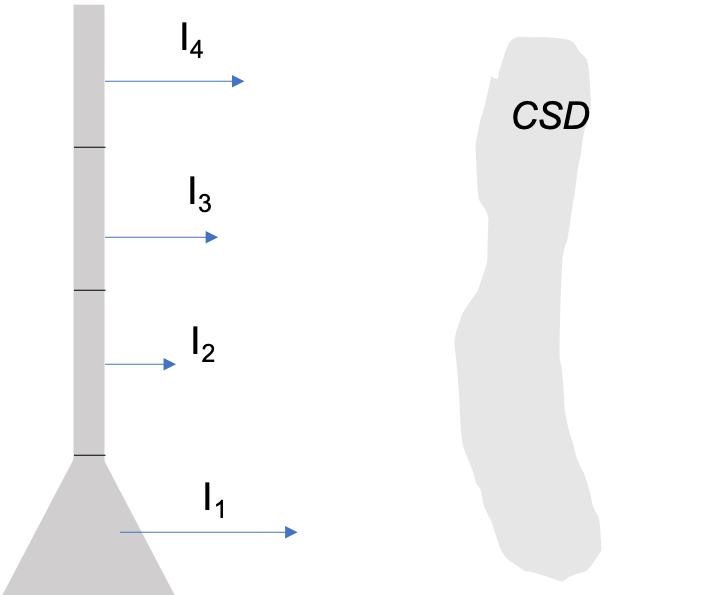
\includegraphics[width=0.5\textwidth]{Figures/VC/CSD.png}
\end{center}
\caption{\textbf{Neuronal current sources.}  {\bf (A)} When simulated on a numerical scheme, the transmembrane currents are known at a discrete set of neuronal segments, i.e., as a set of point sources.  {\bf (B)} As a mathematical generality, we can describe the transmembrane currents as a current source density (CSD) distribution, $C({\bf r},t)$. We note the sum of current entering/leaving a neuron is always zero, so that in {\bf (A)}, we must have that $I_1 + I_2 + I_3 + I_4 + I_5= 0$, and in {\bf (B)} we have that the spatial integral over $C({\bf r},t)$ must be zero at all times.
}
\label{VC:fig:CSD}
\end{figure}
Volume conductor theory is essentially based on current continuity in the extracellular medium, i.e., the requirement that no net current can enter/leave a given point in space. Mathematically, current continuity implies that:
\begin{equation}
\nabla \cdot {\bf i_t}({\bf r}, t) = - C({\bf r}, t),
\label{VC:eq:CSD1}
\end{equation}
which is the same as we postulated previously in eq. \ref{Basics:eq:continuity1}. Here, ${\bf i_t}$ is the extracellular current density through the brain tissue, and $C$ is the current source density. What Eq. \ref{VC:eq:CSD1} essentially tells us, is that if a neuron outputs a current into a (infinitesimal) volume of space (the $C$ term), an equally large current leaves that volume as an extracellular current (the $\nabla \cdot {\bf i_t}$ term).

In this chapter, we shall assume that the extracellular current density is described by Ohm's law (eq. \ref{VC:eq:ohmici}). If we combine Eq. \ref{VC:eq:ohmici} and Eq. \ref{VC:eq:CSD1}, we get:

\begin{equation}
\nabla \left( \sigma_t({\bf r}, t) \nabla \phi({\bf r}, t) \right) = - C({\bf r}, t),
\label{VC:eq:CSD2}
\end{equation}

which simplifies to the more commonly used relation:
\begin{equation}
\sigma \nabla^2\phi({\bf r}, t) = - C({\bf r}, t),
\label{VC:eq:CSD3}
\end{equation}
in the less general case where the conductivity $\sigma_t$ is constant. Hence, if we know the distribution of neuronal current sources, we can integrate eq. \ref{VC:eq:CSD2} or eq. \ref{VC:eq:CSD3} to predict the electrical potential in the extracellular space surrounding the sources. 

As indicated above, the variables ${\bf i_t}$, $\sigma_t$ and $\phi$ can in general be functions of both position and time. However, for the remainder of this chapter, we shall for simplicity assume that $\sigma_t$ is constant. Furthermore, it is implicit in eq. \ref{VC:eq:CSD2} that the relationship between current sources and extracellular potentials is instantaneous (i.e., we can solve eq.  \ref{VC:eq:CSD2} at each time point independently), and in the remainder of the chapter we therefore only use the positional argument for ${\bf i_t}$ and $\phi$. 

In the following subsections, we show how VC-theory is used to compute $\phi$ in some idealized cases with a homogeneous extracellular medium, and then discuss how this theory can be expanded to more complex cases accounting for inhomogeneities. 


%%%%%%%%%%%%%%%%%%%%%%%%%%%%%%%%
\section{\blue{Infinite isotropic homogeneous extracellular medium}}
\label{sec:VC:isohomo}
\index{Conductivity!Homogeneous and isotropic}
%%%%%%%%%%%%%%%%%%%%%%%%%%%%%%%%

We shall now derive an expression for the extracellular potential $\phi$ in the case where the extracellular medium is infinite, isotropic and homogeneous. By homogeneous we mean that the conductivity $\sigma_t$ is the same everywhere in space, and by isotropic we mean that $\sigma_t$ is the same in all spatial directions. Although the extracellular medium in reality is neither infinite, nor strictly isotropic and homogeneous, this approximation may still in many cases give fairly good predictions of $\phi$.


%%%%%%%%%%%%%%%%%%%%%%%%%%%%%%%%
\subsection{\blue{Point source approximation}}
\label{sec:VC:pointsource}
\index{Point source approximation}

%%%%%%%%%%%%%%%%%%%%%%%%%%%%%%%%
We start by deriving the contribution to $\phi$ from a single neuronal point source $I_k$ at the point ${\bf r_k}=0$ (Fig. \ref{VC:fig:pointsource}A). 

\begin{figure}[!ht]
\begin{center}
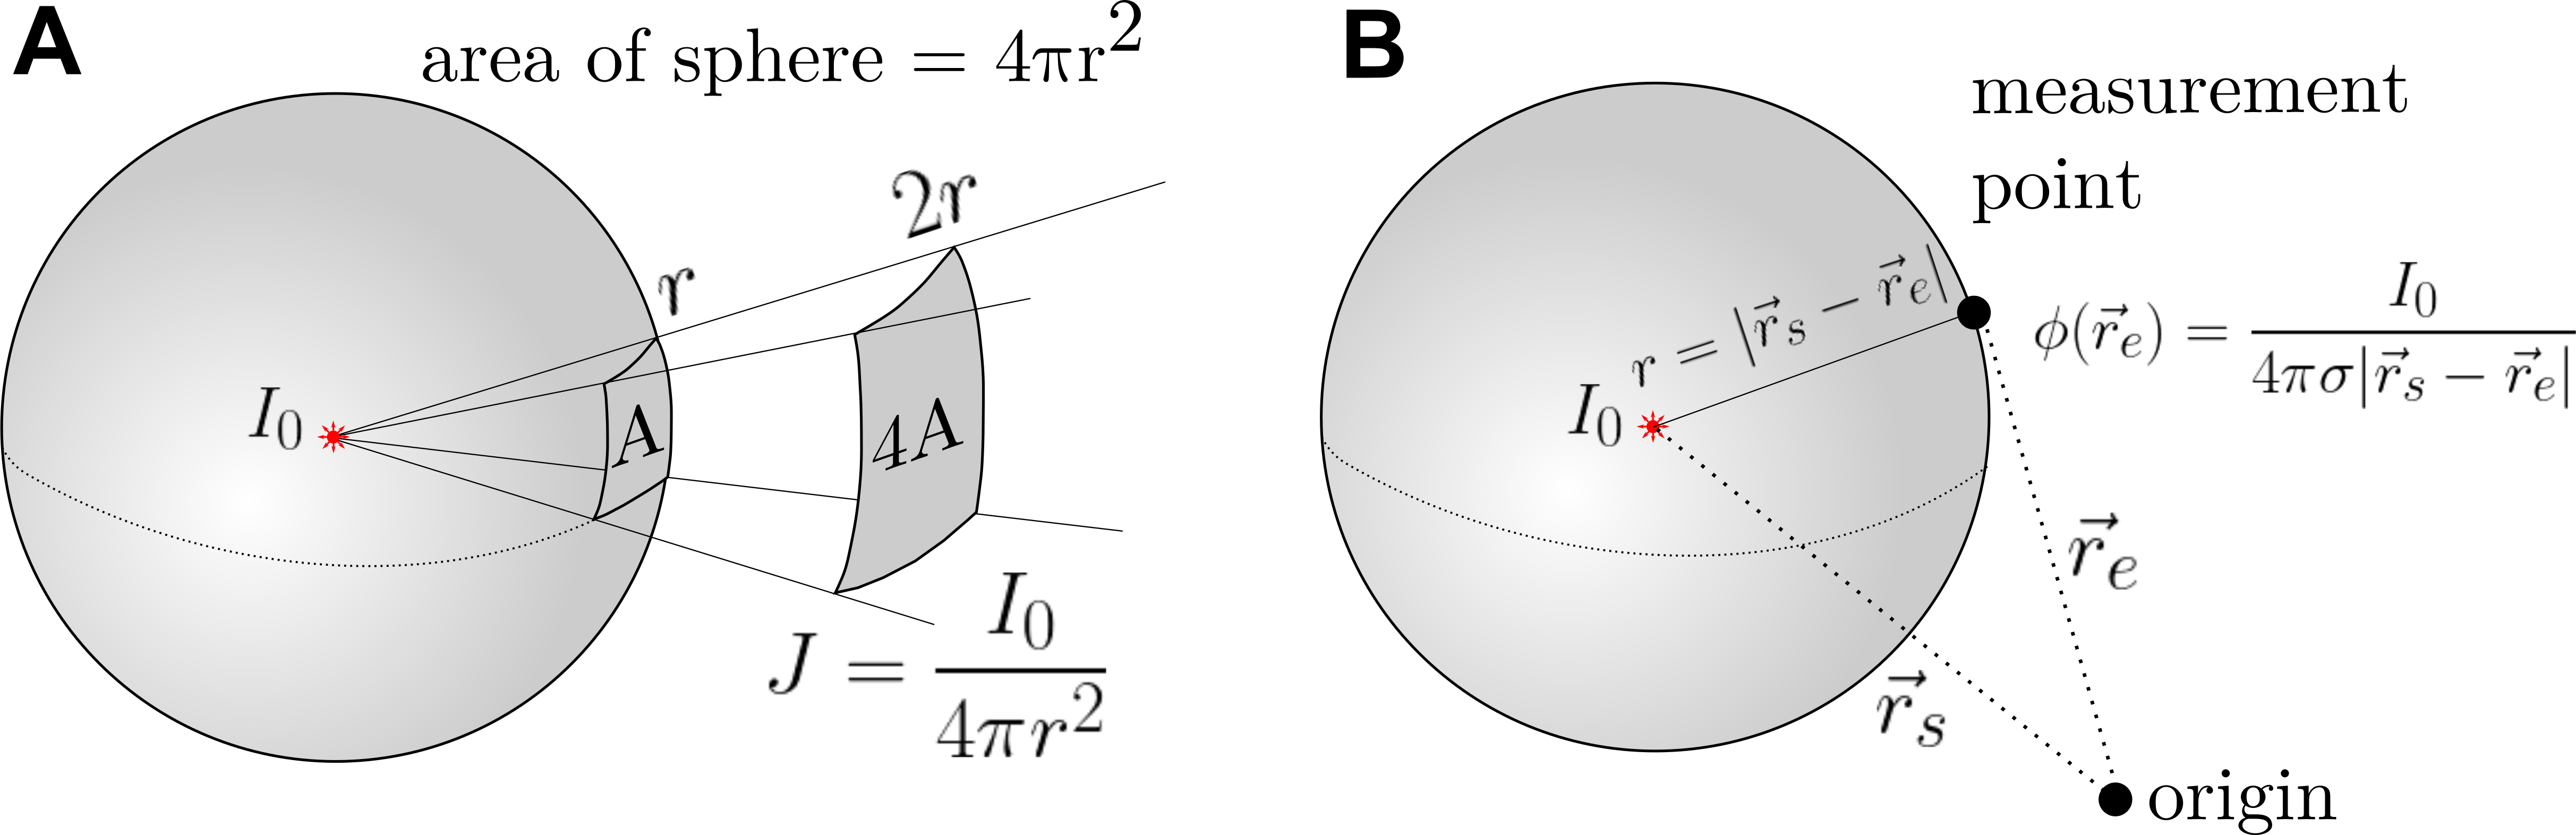
\includegraphics[width=0.8\textwidth]{Figures/VC/EP_from_pointsource_illustration.png}
\end{center}
\caption{\textbf{Extracellular potential from single neuronal point source current.} 
\tvnnote{Har laget utkast til figur. Noe slikt? } \ghnote{Praktfull, men trenger index $t$ paa $\sigma_t$, og $i_t$ erstatter J.}
}
\label{VC:fig:pointsource}
\end{figure}

Here, we could compute $\phi$ by solving eq. \ref{VC:eq:CSD3}. However, due to the spherical symmetry of this simple case, we can take a shorter path by realizing that the current density (eq. \ref{VC:eq:ohmici}) must radially directed, and that its magnitude must be solely a function of distance $r$ from the source:

\begin{equation}
i_t({\bf r}) = i_t(r) = -\sigma_t \frac{d\phi(r)}{dr}.
\end{equation}

Knowing this, we may find $\phi$ by simply demanding that net current $I_k$ injected into the center of the spherical volume with radius $r$ must equal the net current leaving through the surface of the volume, which in turn must equal the current density $i_t(r)$ at the surface multiplied with the surface area $4\pi r^2$. We then get the relationship:

\begin{equation}
I_k = -4\pi \sigma_t r^2  \frac{d\phi(r)}{dr} \, \iff \, \frac{d\phi(r)}{dr} = -\frac{I_k}{4\pi \sigma_t r^2 }.
\label{VC:eq:knut}
\end{equation}

To obtain the final solution for $\phi$, we integrate eq. \ref{VC:eq:knut} from $r$ to $\infty$:

\begin{equation}
\int_r^{\infty} \frac{d\phi(r')}{dr'} dr' = \int_r^{\infty} -\frac{I_k}{4\pi \sigma_t r'^2 } dr'.
\label{VC:eq:knut2}
\end{equation}
Since $\phi({\infty}) = 0$, this leads to the final expression:

\begin{equation}
\phi({\bf r}) = \phi(r) = \frac{I_k}{4\pi \sigma_t r},
\label{VC:eq:pointsource}
\end{equation}
where $r$ is the distance from the source.

In the above, we made things simple by assuming that the current source was placed in the origin ${\bf r} = 0$. For a point source located in an arbitrary point ${\bf r_k} $, the corresponding expression for the extracellular potential is:

\begin{equation}
\phi({\bf r}) = \frac{I_k}{4\pi \sigma_t |{\bf r-r_k}|},
\label{VC:eq:pointsource2}
\end{equation}

If we have several point-current sources, $I_{1}, I_2, I_3, ... $ in locations ${\bf r_1}, {\bf r_2}, {\bf r_3} ... $), their contributions add up linearly, and the potential in a point ${\bf r}$ is given by:

\begin{equation}
\phi({\bf r}) = \frac{I_1}{4\pi  \sigma_t {\bf |r-r_1|}} + \frac{I_2}{4\pi  \sigma_t {\bf |r-r_2|} } + \frac{I_3}{4\pi  \sigma_t {\bf |r-r_3|} } + ... = \sum_k \frac{I_k}{4\pi  \sigma_t {\bf |r-r_k|} }.
\label{VC:eq:pointsources}
\end{equation}


%%%%%%%%%%%%%%%%%%%%%%%%%%%%%%%%
\subsection{\blue{Line source approximation}}
\label{sec:VC:linesource}
\index{Line source approximation}

%%%%%%%%%%%%%%%%%%%%%%%%%%%%%%%%
Eq.~\ref{VC:eq:pointsources} is referred to as the point-source approximation \cite**{Holt1999,Pettersen2008a}, since it approximates the neuron as a set of point current sources, i.e., the neuron delivers to the extracellular space a singular current source per neuronal segment, located in the segment midpoint. 

A more sophisticated choice may be to assume that the transmembrane current is evenly distributed over the segment axis, a choice which is referred to as the line-source approximation \cite**{Holt1999,Linden2014}. The contribution to the extracellular potential from a current $I_k$ in a segment $k$ can be found analytically by integrating eq. \ref{VC:eq:pointsource} over the center-line axis of the compartment (see Appendix C in \cite**{Holt1998}). We here skip the derivation, but give the final solution. For a segment with length $\Delta s_k$, the contribution to the extracellular potential will be:

\begin{equation}
\phi({\bf r},t)_k = \frac{I_k}{4\pi \sigma_t} \int \frac{dr_k}{|{\bf r-r_k}|} = 
\frac{I_k}{4\pi \sigma_t \Delta s_k} \log \left| \frac{\sqrt{h_k^2+\rho_k^2}-h_k}{\sqrt{\ell_k^2+\rho_k^2}-\ell_k} \right|,
\label{VC:eq:linesource}
\end{equation}

Here $\rho_k$ is the distance perpendicular to the line segment, $h_k$ is the longitudinal distance from the end of the segment, and $\ell_k = \delta s_k + h_k$ is the longitudinal distance from the start of the segment (Fig.~\ref{VC:fig:line_source_illustration}). Eq. \ref{VC:eq:linesource} and Eq. \ref{VC:eq:pointsource} are the equivalent expressions where the transmembrane currents in a single neuronal segment are treated as a line source and point source, respectively. As for the point-source approximation, the contributions from several line-sources add up linearly. That is, if we have multiple segments $k$, the extracellular potential can be computed as:

\begin{equation}
\phi({\bf r},{\bf t}) = \sum_k \frac{I_k}{4\pi \sigma_t \Delta s_k} \log \left| \frac{\sqrt{h_k^2+\rho_k^2}-h_k}{\sqrt{\ell_k^2+\rho_k^2}-\ell_k} \right|,
\label{VC:eq:linesources}
\end{equation}

\begin{figure}[!ht]
\begin{center}
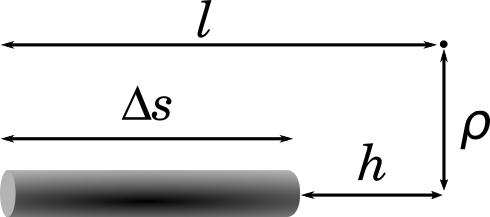
\includegraphics[width=0.5\textwidth]{Figures/VC/line_source_illustration.png}
\end{center}
\caption[]{\textbf{Line-source approximation.} Definitions of symbols used in the line-source approximation. }
\label{VC:fig:line_source_illustration}
\end{figure}

The line-source approximation can be expected to give a better prediction of $\phi$ than the point-source approximation at points in space that are very near neuronal membranes, especially when it comes to predicting rapid fluctuations in $\phi$, such as the extracellular action potential signature \cite**{Holt1999}. At points further away from membranes, the two approaches give converging predictions, see Fig.~\ref{VC:fig:point_vs_linesource}.

\begin{figure}[!ht]
\begin{center}
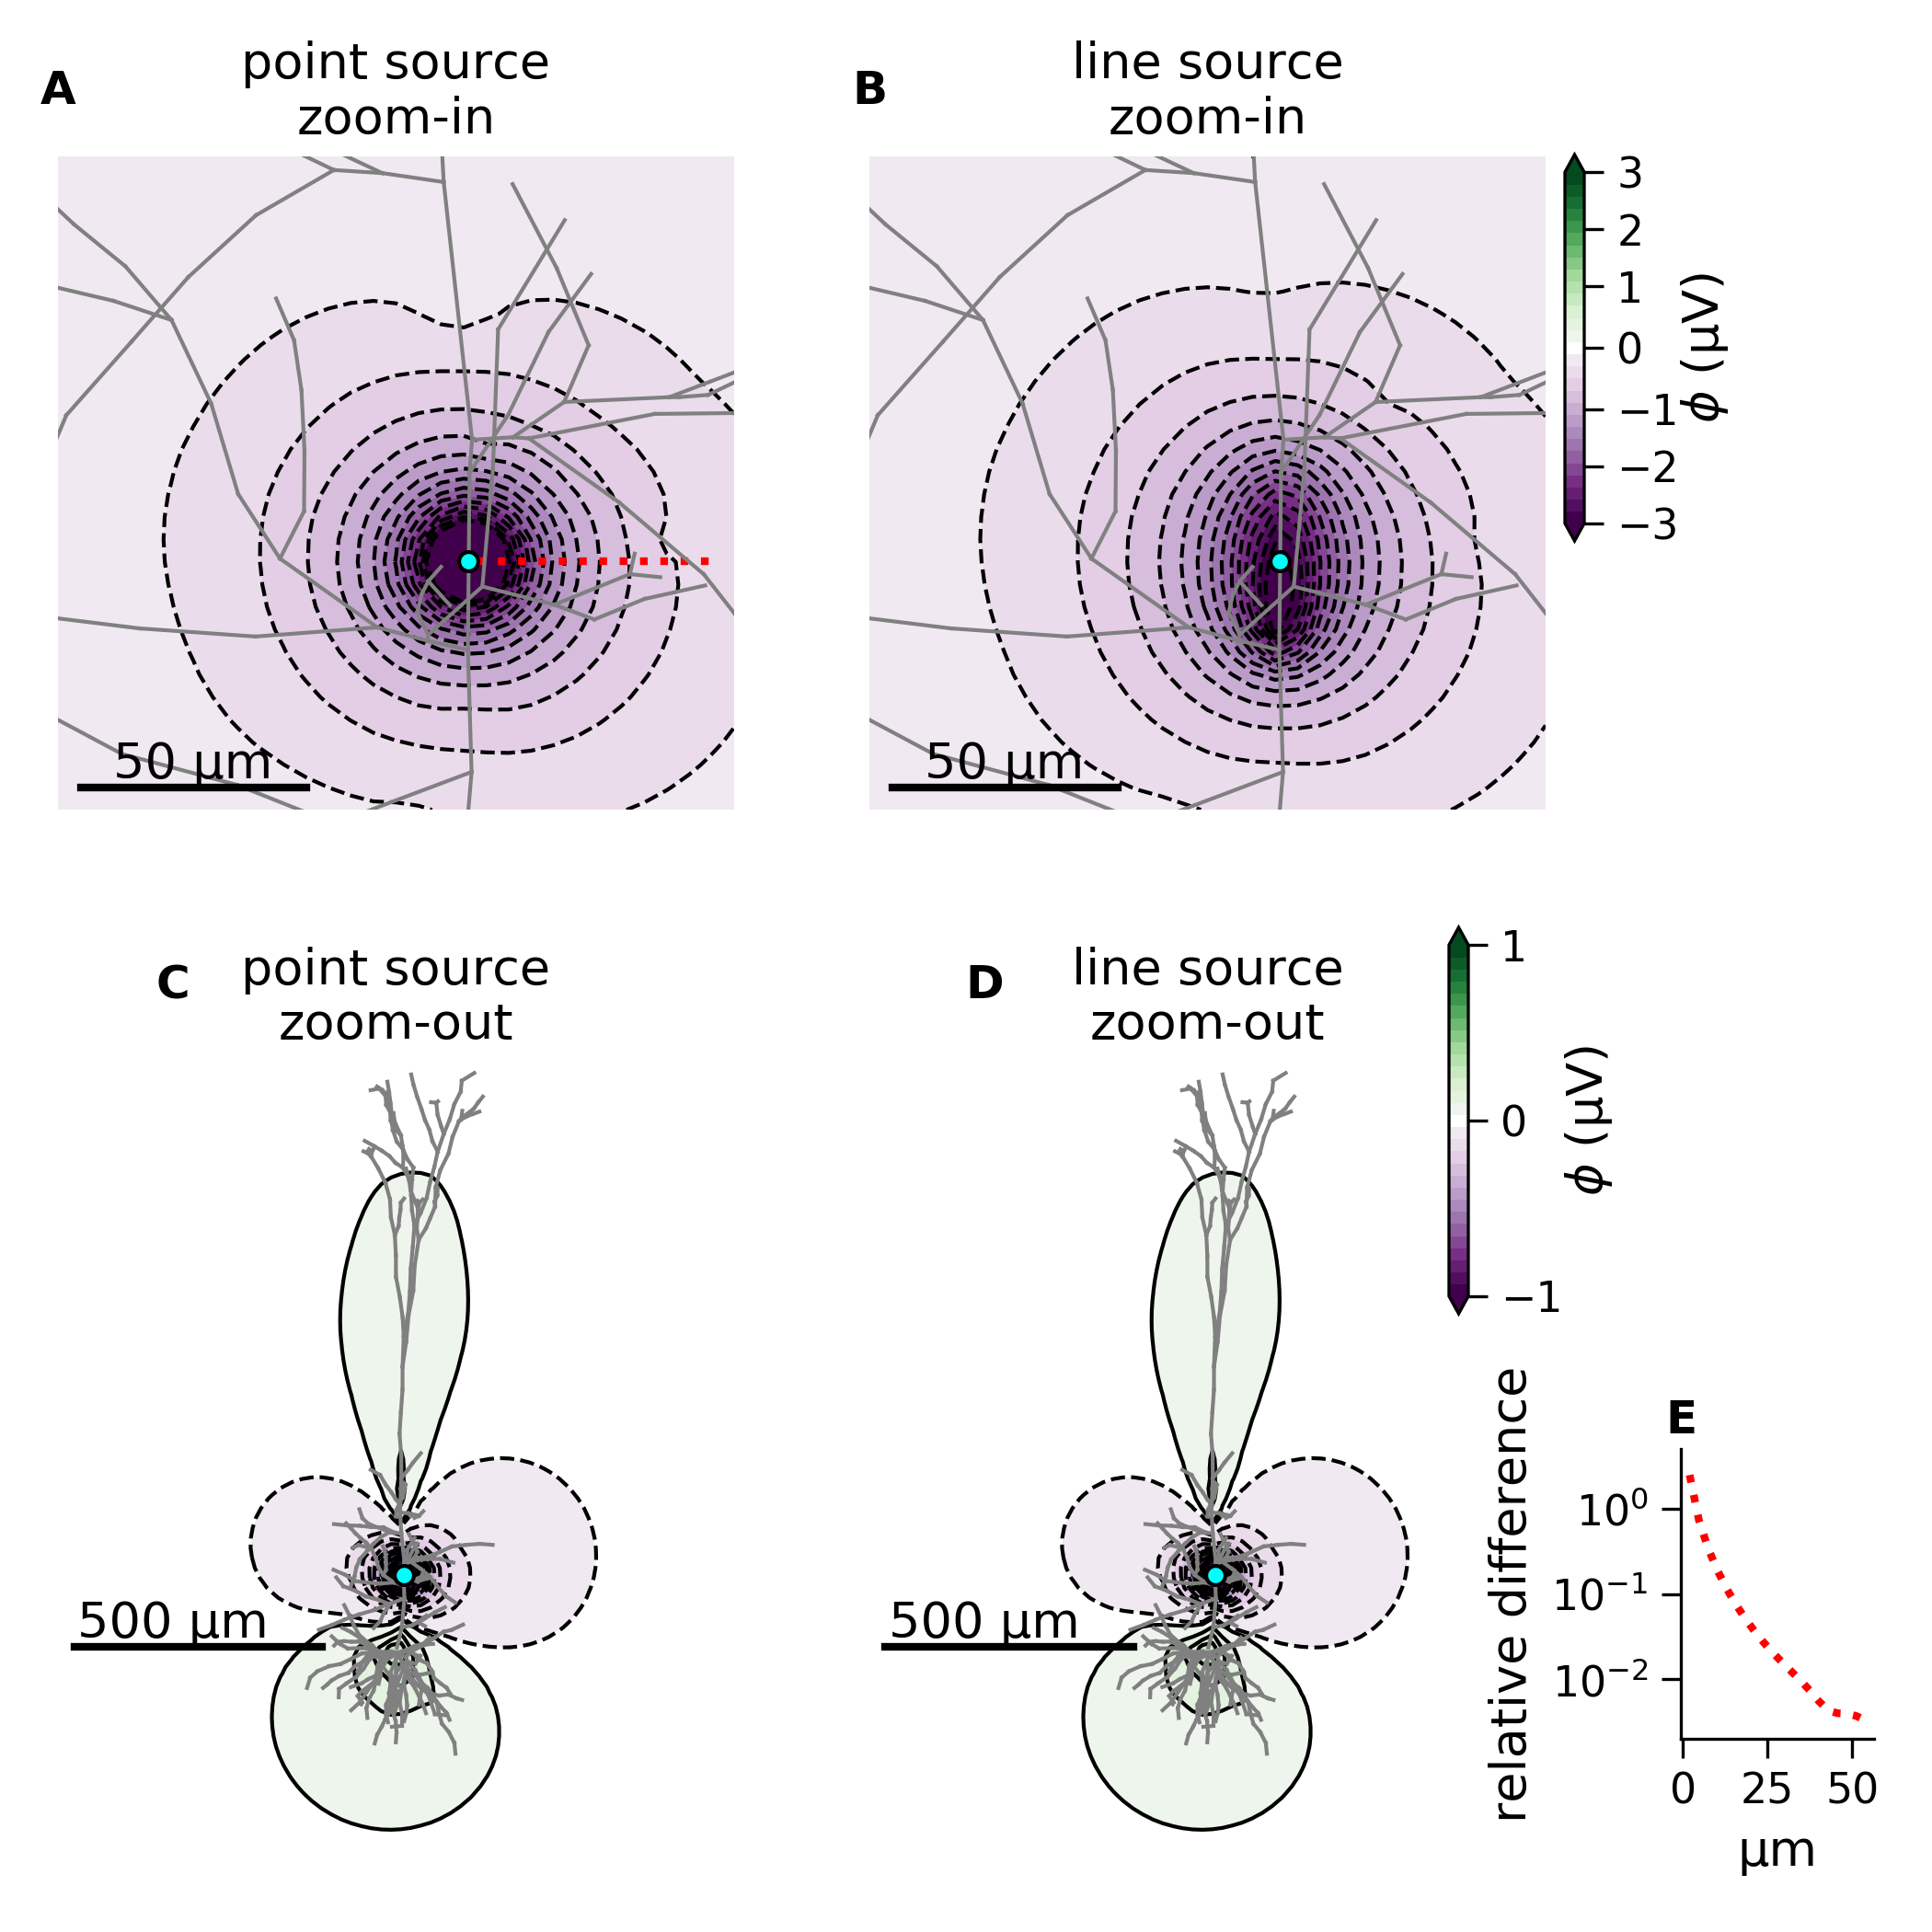
\includegraphics[width=0.7\textwidth]{Figures/VC/fig_point_versus_linesource.png}
\end{center}
\caption[]{\textbf{Point- versus line-source approximation.} \ghnote{Very nice, but I suppose we need to write some words about these simulations, use of neuron model etc?}
}
\label{VC:fig:point_vs_linesource}
\end{figure}

%%%%%%%%%%%%%%%%%%%%%%%%%%%%%%%%
\subsection{\blue{Current-source-density description}}
\label{sec:VC:CSD}
\index{Current source density}
%%%%%%%%%%%%%%%%%%%%%%%%%%%%%%%%
The forward modelling formulas in Eq. \ref{VC:eq:pointsources} and \ref{VC:eq:linesources} can be expressed more generally in terms of the CSD. The starting point is then eq. \ref{VC:eq:CSD3}, which for a homogeneous and isotopic medium can be written: 

\begin{equation}
\nabla^2 \phi({\bf r}) = - \frac{C({\bf r})}{\sigma_t}
\label{VC:eq:CSD4}
\end{equation}

Since this is a linear differential equation, we may solve it by first finding its Green's function, i.e., the solution to an impulse response $C({\bf r}) = I' \delta^3({\bf r-r'})$, 
\ehnote{lite fan av notasjon med $'$, siden dette oftest brukes om den deriverte.}
where $\delta^3({\bf r})$ is the Dirac delta function in three dimensions, and $I'$ is the current source at this location. The general solution can then be expressed as a convolution over such Green's functions. Thus, we first seek the solution to: 

\begin{equation}
\nabla^2 \phi({\bf r}) = - \frac{I' \delta^3({\bf r-r'})}{\sigma_t}.
\label{VC:eq:CSD5}
\end{equation}

We already listed the solution to this in eq. \ref{VC:eq:pointsource2}, but we here provide a more rigorous derivation. We start by by integrating both sides of eq. \ref{VC:eq:CSD5} over an arbitrary 3D volume containing the source:

\begin{equation}
\iiint_V \nabla^2\phi({\bf r}) \,dV =  - \frac{I'}{\sigma_t} \iiint_V \ \delta^3({\bf r-r'}) \, dV,
\label{VC:eq:marit}
\end{equation}

By the definition of the delta-function, the right hand side of equation \ref{VC:eq:marit} is simply $I'/\sigma$. Using Gauss' theorem, we can convert the volume integral on the left hand side of eq. \ref{VC:eq:marit} to a surface integral, so that eq. \ref{VC:eq:marit} becomes:

\begin{equation}
\oiint_{S} \nabla\phi({\bf r}) \cdot \, d{\bf S}  = - \frac{I'}{\sigma_t},
\label{VC:eq:berit1}
\end{equation}

To solve this, it is convenient to chose the volume that we integrate over to be a sphere centered at the source location ${\bf r'}$, and with radius $R = |{\bf r-r'}|$ (Fig. \ref{VC:fig:pointsource}B). Due to the symmetry of problem, we then know that the electrical potential is the same for all ${\bf r}$ on the surface of the sphere, so that $\phi({\bf r}) = \phi(R)$. We also know that its gradient $\nabla\phi({\bf r}) = d\phi(R)/dR$ is constant over the surface, and perpendicular to the surface increment $d{\bf S}$. If we use this, eq. \ref{VC:eq:berit1} becomes:
\begin{equation}
\oiint_{S} \frac{d\phi(R)}{dR} d{S}  = - \frac{I'}{\sigma_t},
\label{VC:eq:berit1ogenhalv}
\end{equation}
which has the solution:
\begin{equation}
4\pi R^2 \frac{d\phi(R)}{dR} = \frac{I'}{\sigma_t}
\label{VC:eq:berit2}
\end{equation}
If we integrate this from $R$ to $\infty$, and use that $\phi(\infty) = 0$, we get:
\begin{equation}
\phi(R) = \phi({\bf r}) = \frac{I'}{4\pi \sigma_t R}.
\label{VC:eq:berit3}
\end{equation}
We may now insert back for $\phi(R)= \phi({\bf r})$ and $R = |{\bf r-r'}|$ to obtain the desired Green's function:

\begin{equation}
\phi({\bf r})= \frac{I'}{4\pi \sigma_t |{\bf r-r'}|},
\label{VC:eq:berit4}
\end{equation}
As earlier stated, the solution for a general CSD can be expressed as a convolution over the Green's function, so that:

\begin{equation}
\phi({\bf r}) = \frac{1}{4\pi \sigma_t}\iiint_V \frac{C({\bf r'})}{|{\bf r}-{\bf r'}|} \,dV, 
\label{VC:eq:csds}
\end{equation}
where the volume integral runs over all sources. Here, $C$ represents whatever approximation one used for the current sources, and eq. \ref{VC:eq:csds} is the continuous counterpart to eq. \ref{VC:eq:pointsources}. If we describe the CSD as a sum of point sources, i.e.,  $C({\bf r}) = \sum_k I_k \delta^3({\bf r} - {\bf r_k})$, eq. \ref{VC:eq:csds} reduces to eq.\ref{VC:eq:pointsources}.


%%%%%%%%%%%%%%%%%%%%%%%%%%%%%%%%
\section{\orange{SN: Dipole approximation}}
\label{sec:VC:dipole}
\ghnote{GH: Jeg skrev en skisse til dette kapittelet, men fint om SN kan gaa gjennom.}
\ehnote{Jeg ville skrevet dette ut fullt likt som under "Spherical form" paa Wikipedia https://en.wikipedia.org/wiki/Multipole\_expansion}
%%%%%%%%%%%%%%%%%%%%%%%%%%%%%%%%
The \textit{dipole approximation} \index{Dipole approximation} is an alternative to eq. \ref{VC:eq:pointsources} for predicting the extracellular potential. The approximation is good provided that the "measuring point" for $\phi$ is far away from the source-sink distribution that it originates from, like in the case of EEG.

To be more precise, if the distance from the center of the volume containing the current sources to the measurement point is larger than the maximal distance from volume center to any source [cite - find Jackson!], we can reformulate eq. \ref{VC:eq:pointsources} by using the the multipole expansion \cite**{Nunez2006}:

\begin{equation}
\phi(R) = \frac{C_{monopole}}{R} + \frac{C_{dipole}}{R^2} + \frac{C_{quadrupole}}{R^3} + \frac{C_{octupole}}{R^4} + ...
\label{VC:eq:multipole}
\end{equation}
where $R$ is the distance from the center of the source distribution, $C_{monopole}$ is the monopolar contribution of the CSD to $\phi$, $C_{dipole}$ is the dipolar contribution from the CSD to $\phi$, and so on. The derivation of this expression can be found in Appendix \ref{app:dipoleappendix}. 

As we explained in Section \ref{sec:Neuron:membranecurrents}, the net sum of currents over a neuronal membrane is always zero, meaning that the monopolar contribution, i.e., first term in eq. \ref{VC:eq:multipole}, vanishes. Furthermore, the quadrupole, octopole and higher-order contributions to $\phi$ decay rapidly with distance $R$. Provided that we are sufficiently far away from the source distribution, $\phi$ can therefore be well approximated by dipole contribution alone:

\begin{equation}\label{VC:eq:CDA}
\Phi(\mathbf{R}) \approx \frac{1}{4 \pi \sigma_t} \frac{|\mathbf{p}| \cos \theta}{R^2},
\end{equation}
where we have expressed $C_{dipole}$ in terms of the current dipole moment ($\mathbf{p}$), the angle ($\theta$) between the current dipole moment and the distance vector ($\mathbf{R}$), as explained in Appendix \ref{app:dipoleappendix}. 

The current dipole moment is a function of the sum of all the transmembrane currents in a neuron \cite**{Pettersen2008,Pettersen2014,Nunez2006}: 
\begin{equation}\label{VC:eq:dipole}
\mathbf{p} = \sum_{k=1}^N I_k \mathbf{r}_k.
\end{equation}
For example, if we have a simple two-compartmental (and purely dipolar) neuron with a current sink $-I$ at location $\mathbf{r}_1$ and a current source $I$ at location $\mathbf{r}_2$, the current dipole moment can be formulated as $\mathbf{p} = -I\mathbf{r}_1 + I\mathbf{r}_2 = I(\mathbf{r}_2 - \mathbf{r}_1) = I\mathbf{d}$. Here $\mathbf{d}$ is the distance vector between the current sink and the current source, giving the length $d$ and direction of the current dipole. 

As we mentioned above, the current dipole approximation is only applicable when we are at some distance away from the source distribution. As a rule of thumb, the approximation is though to be good when $R$ is three to four times greater than the dipole length: $R > 3d$ or $R > 4d$ \cite**{Nunez2006}. It has been found to work well for predicting the extracranial EEG signal, but less well for intracranial electrocorticography (ECoG) \cite**{naess2020biophysical}.


\section{\orange{TVN: Modelling recording electrodes}}
\label{sec:VC:electrodes}
\index{Electrode model}

\gen{Kanskje det kunne v�re en ide � ogs� beskrive methods-of-imaging og modellering i MEAs her?
Hadde f�rst tenkt � ta det med i Spikes-kapitlet. Men den gjelder jo like mye for LFP og har blitt brukt av oss i denne 
sammenheng i flere prosjekter med  Ness eller Pettersen som f�rsteforfatter.}

We have demonstrated how we can use VC theory to make predictions about the extracellular potentials at any point in space following some neural activity. However, in experiments these extracellular potentials must be measured through some kind of measurement electrode. The presence of such a measurement electrode might itself affect the measured potentials in several different ways, depending on both the electrode and the extracellular potential that is being measured. Here we present a short review of different approaches to model such effects.

\tvnnote{Litt usikker på om jeg bruker alle begreper riktig i dette avsnittet} Recording electrodes essentially consist of an electrode surface in direct contact with neural tissue, connected with a wire to an amplifier that measures the potential relative to a reference electrode \cite**{Martinsen2008}, see Fig.~\ref{VC:fig:elec_circuit}. For recording electrodes to accurately measure the potential at the electrode surface, the measurement electrodes themselves must have a very high conductivity so that no potential drop occurs from the measurement site to the amplifier. The electrodes are therefore typically made of a highly conductive metal like silver or platinum, and the potential directly on the inside of the electrode surface is in practice homogeneous. The amplifier must however have a near zero conductivity, so that a negligible amount of current will cross the tissue-electrode interface, as this can cause electrode polarization effects\index{Electrode polarization} \cite**{Schwan1992,Martinsen2008,Moulin2008,Ishai2013}. The homogeneous potential inside the recording electrode ideally corresponds to a spatial average of the potential across the outer surface of the electrode \cite**{Ness2015,Vermaas2020b}\tvnnote{Bør finne lærebok-referanse til dette?}. 

\begin{figure}[!ht]
\begin{center}
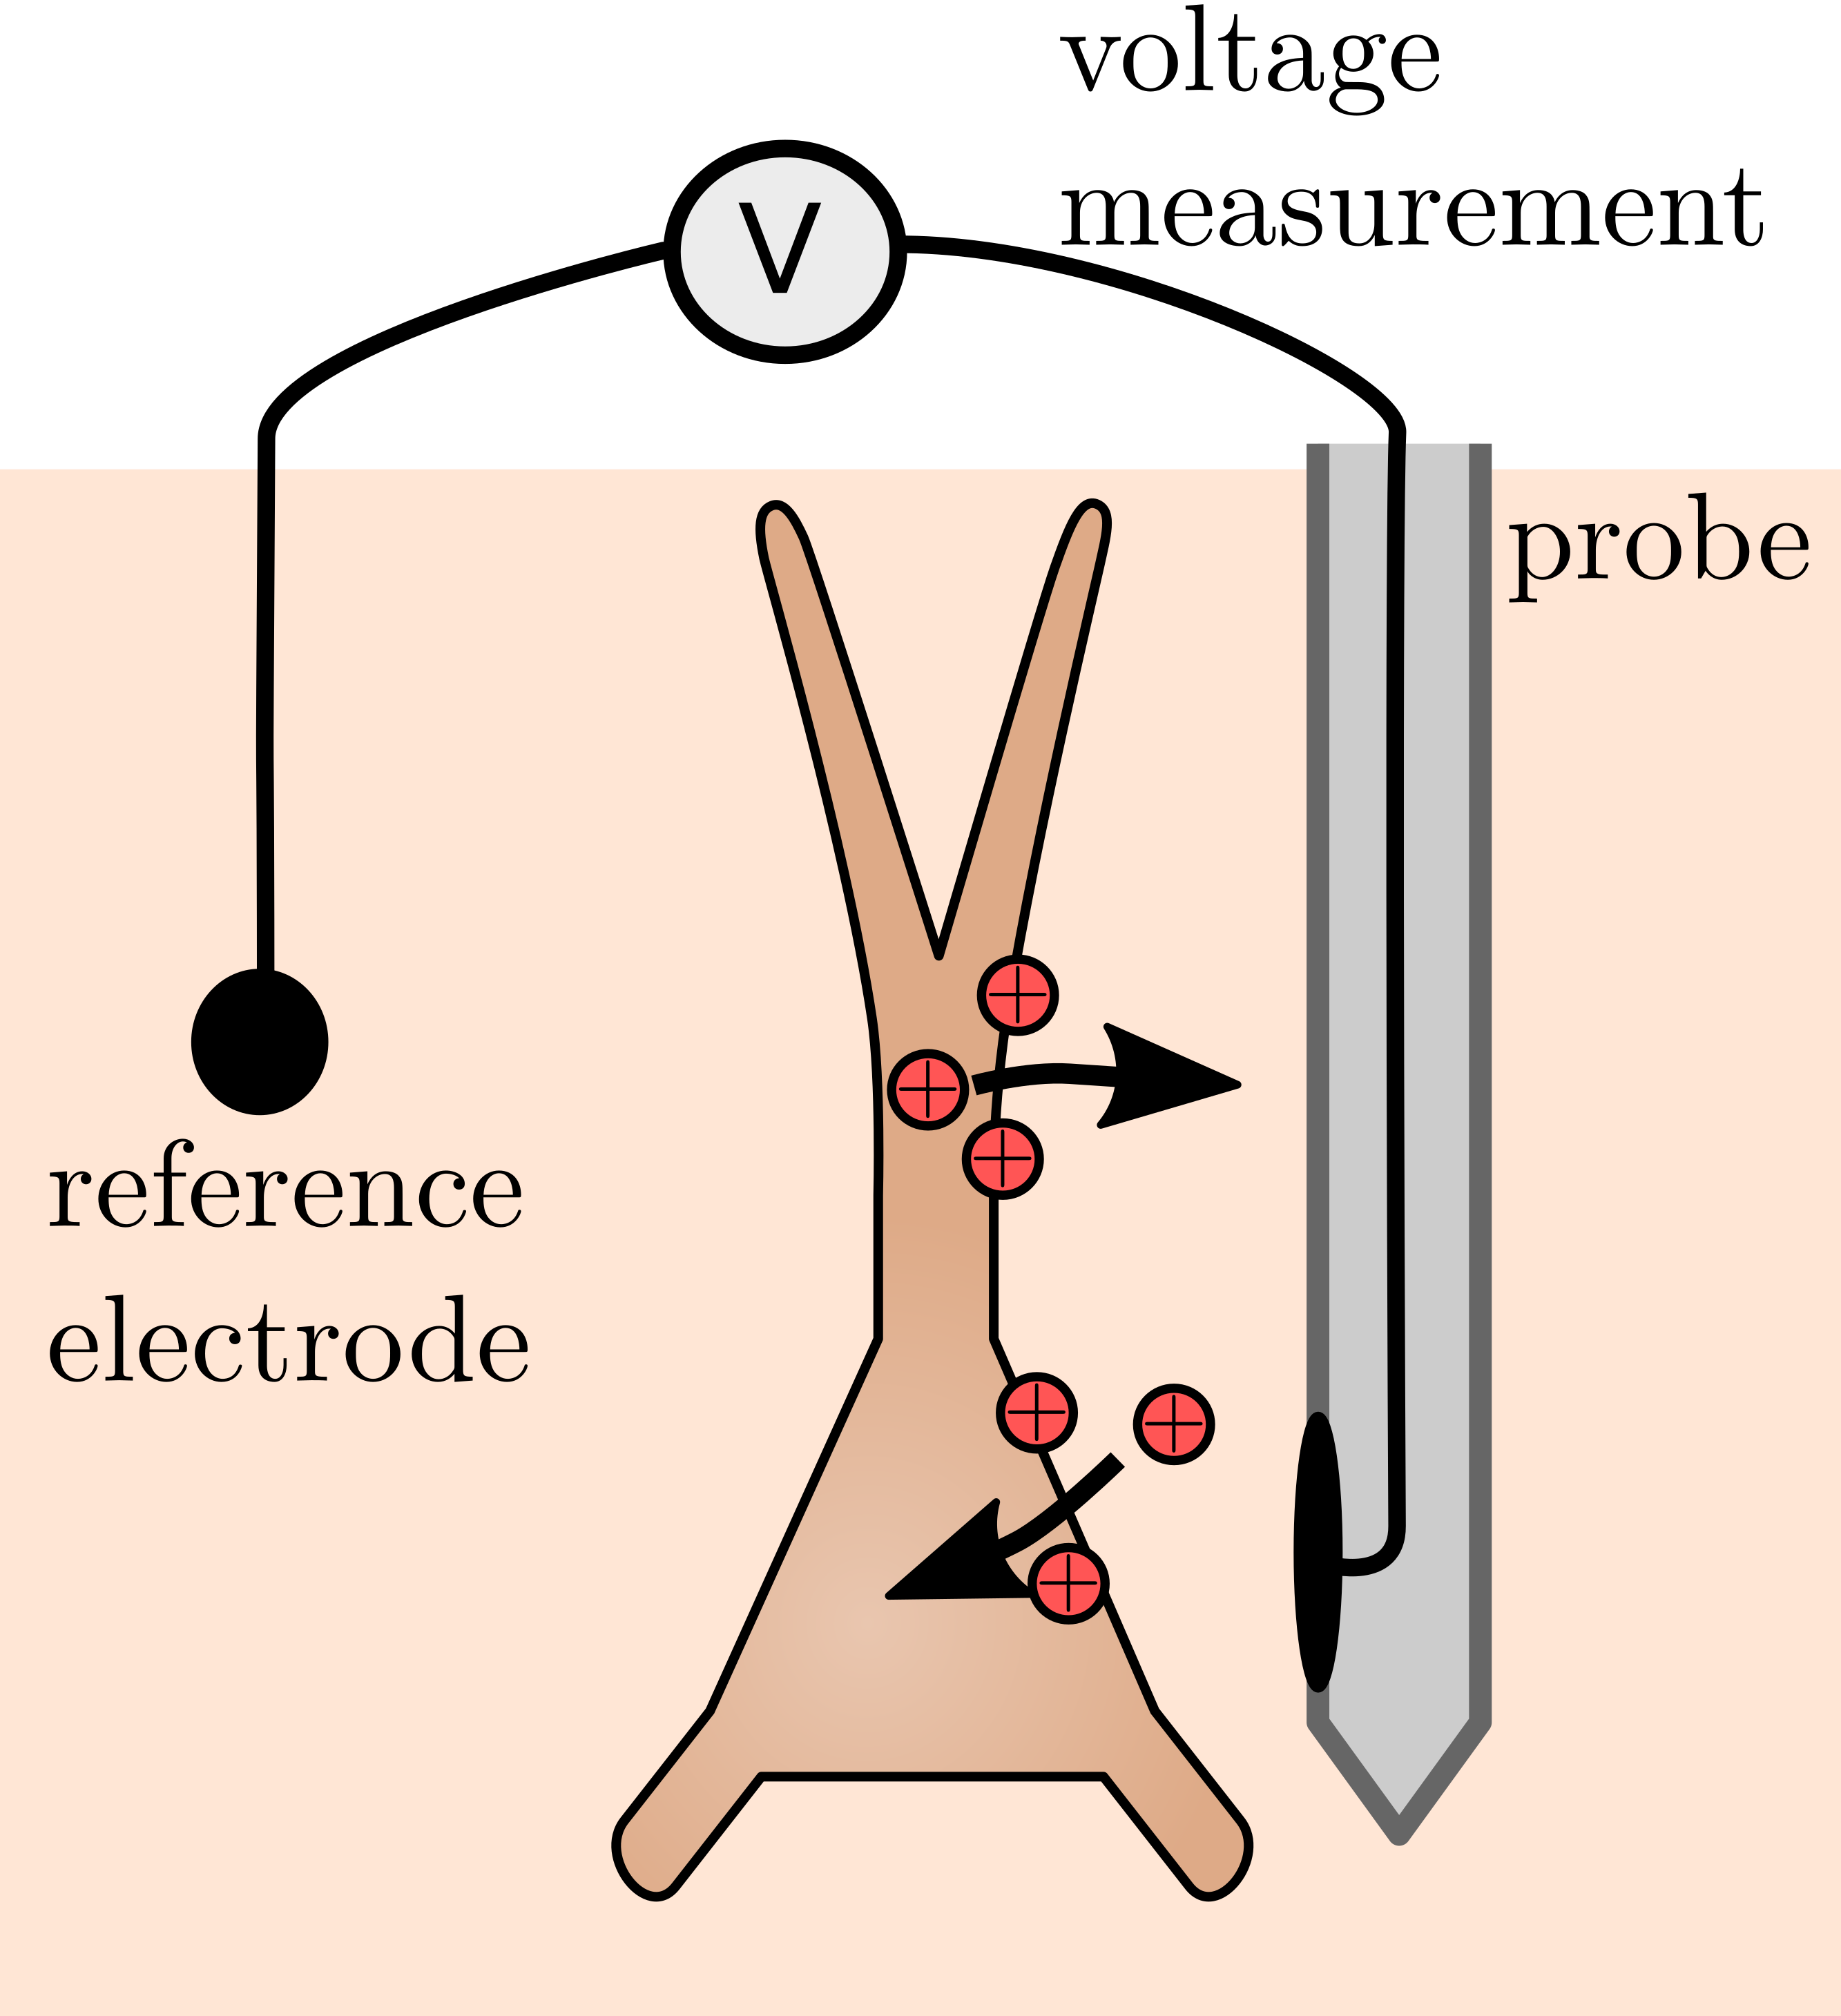
\includegraphics[width=0.4\textwidth]{Figures/VC/rec_elec_circuit.png}
\end{center}
\caption[]{\textbf{Illustration of recording circuit}
Electric potential is measured between recording electrode and reference electrode, and represents the energy required to move a positive test charge from the reference electrode and to the measurement electrode. If, say, positive ions are leaving the extracellular medium (and entering a cell) in the vicinity of the recording electrode, then the energy needed to move a positive charge to the measurement electrode is negative, that is, one can gain energy by moving the charge there.  \ghnote{Litt usikker paa energi-betraktningene her. Dvs. ikke paa om de er riktige, men om de hjeper leseren...}
}
\label{VC:fig:elec_circuit}
\end{figure}

A possible concern is whether the electrode impedance or other electrode properties can distort measured extracellular potentials, through introducing unintentional temporal filtering effects on the recorded potentials. Effectively, this would amount to the potential on the inside of the electrode surface being different from the (spatial average of the) potential on the outside of the electrode, and therefore not represent the "true" extracellular potential. For example, note that \gex{metallic} 
recording electrodes are typically unable to measure static (DC) potentials, or capture changes slower than $\sim$ 0.1 Hz.
\gen{Hvor har vi dette tallet fra?} 
\ehnote{jeg er ogsaa overrasket over at metallelektroder ikke kan maale konstante potensialforskjeller i en loesning (i all den tid det finnes frie ioner i loesningen)?}
Such DC potentials can be present in neural tissue, and can often arise in simulated extracellular potentials from cell models with active conductances, for example because of the $I_{\rm h}$-current \cite**{Ness2016}. In such cases, the simulated baseline (or mean) extracellular potential is typically subtracted from the extracellular potentials to effectively remove the unobservable DC-potential.

Apart from this, it has been convincingly argued that, provided that the proper recording equipment is used, electrode impedance or other electrode properties should not substantially distort recorded potentials \cite**{Martinsen2008,Moulin2008,Nelson2008,Nelson2010}. 
  Note that this only applies to recording electrodes, and that substantially more complex electrode models might be needed to accurately represent current stimulation electrodes because of electrode polarization \cite**{McIntyre2001,Martinsen2008,Joucla2012}.
In essence, the complication stems from that in electronics the electric charge is carried by electrons, while in neural tissue the electric charge is carried by positive and negative ions. For low frequencies, which do not favor capacitive currents, this change of charge carrier can be problematic, resulting in electrode polarization. 
  Modelling electrode polarization effects will often require numerically comprehensive approaches, like the Finite Element Method (FEM) \index{Finite Element Method}\cite**{Buitenweg2003,Moulin2008,Joucla2014,Vermaas2020a}, and/or careful calibration to experimental recordings \cite**{Gabriel1996,Martinsen2008,Miceli2017},
and this topic is not covered here.
\gen{Electrode polarization hadde vel passet best i en section om "Modeling of stimulation electrodes" ikke i naavaerende 
"Modeling of recording electrodes". Og siden vi vel skal ha med tekst om elektrisk stimulering senere saa hadde det kanskje vaert greit med en liten separat section om dette?}

Under the assumption that the proper recording equipment is used \cite**{Nelson2008,Nelson2010}, electrode properties can still affect the recorded potential. For example, if the extracellular potential changes across the outer surface of the recording electrode, this can introduce a spatial filtering effect on the measured potentials. 
\gen{Her maa vi vaere presise. Potensialet paa selve elektroden vil vaere det samme, det som vil variere er hva potensialet ville vaert paa denne "virtuelle" flaten hvis det ikke hadde vaert en metallisk elektrode der.}
In practice, this means for example that extracellular action potentials (which are very spatially confined) will be less prominent on electrodes with diameters larger than $\sim$30~$\mu$m \cite**{Moffitt2005,Moulin2008}, see Fig.~\ref{VC:fig:electrode_size}.

\gen{Har flyttet figuren "Bigger recording electrodes can cause smaller and broader EAPs" til Spikes kapitlet}

%\begin{figure}[!ht]
%\begin{center}
%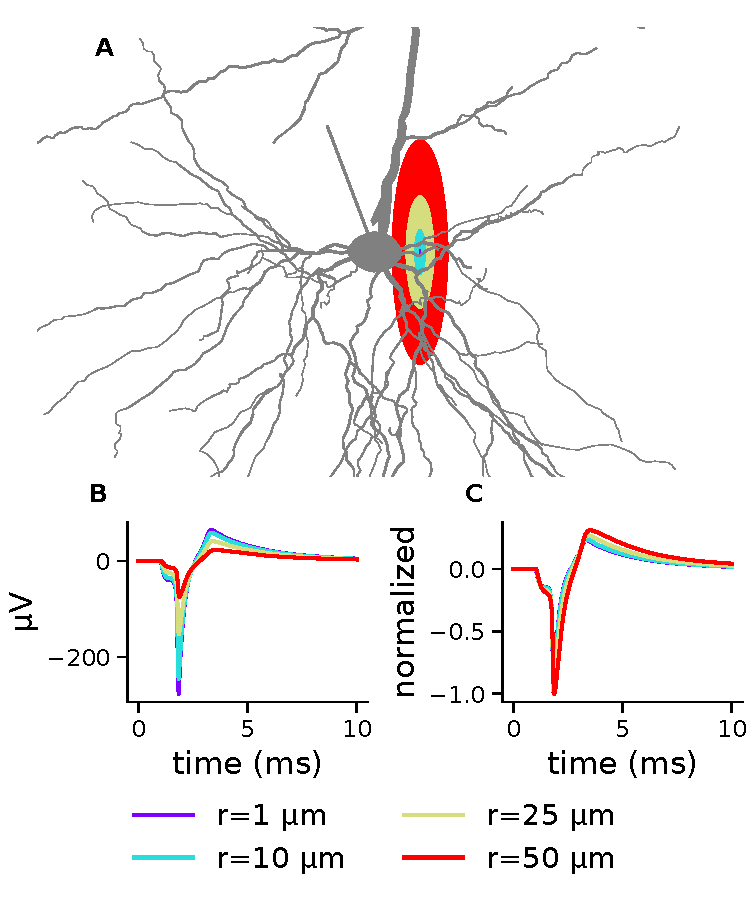
\includegraphics[width=0.6\textwidth]{Figures/VC/fig_elec_size_effect.pdf}
%\end{center}
%\caption[]{\textbf{Effect of electrode size.}Bigger recording electrodes can cause smaller and broader EAPs.  \ghnote{Flott. Kursivere $r$? Forklare simuleringen?}
%\gen{Veldig fin figur, men jeg synes den kan passe enda bedre i "spikes" kapitlet. Hva tenker dere?}}
%\label{VC:fig:electrode_size}
%\end{figure}

\subsection{\orange{Point-electrode approximation}}
\label{VC:sec:point-electrode}
\index{Point-electrode}
The most straightforward and also most common approach when modeling extracellular recordings is to use the ideal point electrode approximation. This corresponds to  
ignoring any potential effect from recording electrodes or electrode shanks, and calculating the extracellular potential  at single points. For relatively small micro-electrodes inserted into neural tissue, this has been found to be a reasonable approximation \cite**{Ness2015,Buccino2019}\tvnnote{Legg til sitering fra ikke-oss}.

\ghnote{Tror vi maa forklare at punktet vaart er et punkt i en coarse-grained beskrivelse av tissue. "Punktet" i vaar utregning tilsvarer en midling over et mikrometerstort omraade rundt punktet s.a. utslaget ikke er avhengiv av hvorvidt det er 1, 2, 3 eller 40 nm til naermeste membran. Den samme midlingen gjoeres av smaa elektroder. Saa "point" betyr i denne sammenhengen at vi allokerer elektrodemaalingen til punktet i sentrum av elektroden, og at elektrodens tilstedevaerelse ikke paavirker hva midlingen over dette omraadet vil vaere?}
\gen{Kan vi ikke ogsaa tenke paa maalingen som maaling av potensialet i et lite punkt i ECS (selv om vi bruker coarse-grained beskrivelse)?}


\subsection{\orange{Disc-electrode approximation}}
\label{VC:sec:disc-electrode}
\index{Disc-electrode approximation}
In some cases recording electrodes are large enough that the extracellular potential varies substantially across the electrode surface. In such cases, we can use the point-electrode approximation to calculate the potential at many points across the electrode surface and compute the average potential. This is typically referred to as the disc-electrode approximation \cite**{Linden2014,Ness2015}. 
\ehnote{Camunas-Mesa and Quiroga (2013) gjorde dette foer oss, og tok i tillegg med kapasitive effekter pluss impedanse for electrode-saline interface basert paa noe teori fra Robinson1968.}

By taking into account the physical extent of the electrodes, the disc-electrode approximation can account for spatial filtering effects. However, very close to electrodes the electrodes can themselves affect the close-by extracellular potential, since they represent a region of a highly conductive material in contact with the tissue being measured from. 
The effect of the presence of highly conductive electrodes can be investigated using FEM, and \citeasnoun**{Ness2015} found that the disc-electrode approximation was fairly accurate for estimating measured potentials from a point current source more than $\sim$2 times the electrode radius away from the electrode. \gen{Kanskje ha med en figur om dette, tilpasset fra Ness2015?}

In certain cases, like in ECoG \index{ECoG} measurements from the cortical surface, the recording electrodes are both large ($\sim$~2-5~mm diameter) and close to the neuronal sources (the thickness of the human cortex is $\sim$3~mm). In such cases the electrode properties can therefore be expected to have large effect on measured potentials, see for example  \cite**{Vermaas2020b,Rogers2020}.

\subsection{\orange{Effect of the electrode probes (shaft?}}

Large multi-contact electrode probes can be expected to have a substantial effect on close-by extracellular potentials, since it represents a large non-conducting volume \cite**{Mechler2012,Buccino2019b}. It has been demonstrated that such large probes can amplify or dampen recorded potentials from nearby cells by almost a factor of two, depending on whether the cell was in front of or behind the electrode shank \cite**{Moffitt2005,Buccino2019b}.

%%%%%%
\section{\blue{Approximations used in VC theory}}
\label{sec:VC:approximations}

\ehnote{For meg fremstaar det som litt rart aa ha disse kapitlene \emph{etter} aa ha introdusert kabellikning, punktkildepotensial, elektrodemodeller etc. Skulle ikke dette vaert i kapt 2?}

%%%%%%%%%%%%%%%%%%%%%%%%%%%%%%%%
The VC theory presented in this chapter relies on several assumptions and approximations. Firstly, the theory is based on the quasi-static approximation of Maxwell's equations (see Section \ref{sec:VC:quasistatic} for more on this). Secondly, the the extracellular medium is assumed to be linear, so that the current density is proportional to the electrical field (see Section \ref{sec:VC:LinEx} for more on this). Thirdly, extracellular currents are assumed to be exclusively due to Ohmic drift, although other currents could in principle be present (see Section \ref{sec:VC:onlyohmic} for more on this). Fourthly, when applying VC theory, one typically assumes that there is no (ephaptic) feedback from extracellular potentials on the neural activity (see Section \ref{sec:VC:ephaptic} for more on this). Finally, the extracellular conductivity was throughout this chapter assumed to be isotropic, homogeneous and frequency independent, but it is possible to relax these assumptions. Given its important role, we have devoted an entire chapter of this book to the extracellular conductivity (Chapter \ref{sec:Sigma}), where we discuss how the VC theory can be applied also to cases with an anisotropic medium and non-homogeneous medium.

\subsection{\blue{Electro-quasistatic approximation of Maxwell's equations}}
\label{sec:VC:quasistatic}
\index{Quasi-static approximation to Maxwell's equations}
For fields in the brain, the typical temporal frequencies are so low that the magnetic induction term, i.e., the time derivative of ${\bf B}$, has a negligible impact on the electric field ${\bf E}$ \cite**{plonsey1967,Gratiy2017}. Maxwell's (macroscopic) equation for the curl of the electric field (eq.  \ref{Basics:eq:Max3}) can then be simplified to:
\begin{equation}
\nabla \times {\bf E} = - \frac{\partial {\bf B}}{\partial t}  \approx 0, 
\label{VC:eq:maxE}
\end{equation}
This is called the electro-quasistatic approximation, and it follows from eq. \ref{VC:eq:maxE} that the quasi-static electric field is conservative, which is a criterion for relating it to an extracellular potential through:
\begin{equation}
{\bf E} = \nabla \cdot \phi,
\label{VC:eq:conservative}
\end{equation}
as we postulated earlier (eq. \ref{Basics:eq:EV}). 

In contrast, the displacement current term $\partial E/\partial t$ in Maxwell's (macroscopic) equation for the curl of the magnetic field (eq. \ref{Basics:eq:Max4}) is responsible for the charging up of capacitive neural membranes. Therefore, we can not as a generality assume that brain tissue is magneto-quasistatic. However, in shall assume that the extracellular currents are (see Section \ref{sec:VC:onlyohmic}).


\begin{equation}
\nabla \times {\bf H} = {\bf i_t} + \frac{\partial {\bf D}}{\partial t} \approx {\bf i_t},
\label{VC:eq:maxB}
\end{equation}
which is the quasi-\textit{magnetoelectrostatic} approximation. We have here inserted the tissue volume current density ${\bf i_t}$, and not a general current density ${\bf i}$, which might include neuronal curre

since we have excluded the possible membrane current sources.

We may recall the constitutive relations ${\bf D} = \epsilon{\bf E}$ and $\mu{\bf H} = {\bf B}$, with $\mu$ and $\epsilon$ being the permeability and permittivity of the medium, respectively. The assumption behind eq. \ref{VC:eq:maxB} it is that the time variations in the electric field are too slow to affect the magnetic field. If we take the gradient of both sides of this equation, we get that (since the gradient of a curl is zero): 
\begin{equation}
\nabla\cdot {\bf i} = 0, 
\label{VC:eq:maxBstatic}
\end{equation}
which we have also postulated earlier (eq. \ref{Basics:eq:MaxElectroneutral}). 

 For linear materials with instantaneous response properties, 



\begin{equation}
\nabla \cdot {\bf i_t}({\bf r}, t) = - C({\bf r}, t),
\label{VC:eq:CSD1}
\end{equation}


In the previous subsection, we said that eq. \ref{Basics:eq:continuity1} will be our fundamental equation for modeling extracellular potentials. It is therefore important to point out that it is not in disagreement with Maxwell's equations, although eq. \ref{Basics:eq:continuity1} and eq. \ref{Basics:eq:MaxElectroneutral} at a first glimpse may look a bit different. Comparing the two, we we see that in \ref{Basics:eq:continuity1}, ${\bf i}$ has been replaced with ${\bf i_t}$, and a source term $C$ has been added on the right hand side. Essentially, eq. \ref{Basics:eq:continuity1} thus follows from decomposing the total current ${\bf i}$ in eq. \ref{Basics:eq:MaxElectroneutral} into the part of it ($\bf{i_t}$) that runs extracellularly through the tissue and the part of it ($C$) that enters the extracellular space through neural membranes. The reason for making this decomposition is practical. As we shall see in Chapter \ref{sec:VC}, it makes computations easier.
\ehnote{Er vi ikke allerede i kapittel 4? ;-)}


The quasi-static approximation appears to be well-justified for the relatively low frequencies relevant for brain signals, below about 10 kHz \cite**{Nunez2006,Grodzinsky2011}.


\subsection{\blue{Linear extracellular medium} }
\label{sec:VC:LinEx}
\index{Extracellular medium! Linear}

In a linear extracellular medium, the relationship between the current density and the electric field is given by:
\begin{equation}
{\bf i} = \sigma {\bf E}.
\label{VC:eq:bertil}
\end{equation}
This relation is constitutive, meaning that it is observed in nature rather than derived from any physical principle \cite**{Nunez2006,Pettersen2012}. It is quite general, and $\sigma$ can here in principle be anisotropic (i.e., a tensor, accounting for different conductivities in different directions), inhomogeneous (position dependent), and complex (accounting for capacitive effects). We note that eq. \ref{VC:eq:bertil} is generally only valid in the frequency domain, while in the time domain, ${\bf i}$ must be given as a temporal convolution of $\sigma$ and ${\bf E}$ \cite**{Bedard2009}. However, if $\sigma$ is frequency independent (this assumption is discussed further below), eq. \ref{VC:eq:bertil} will also be valid in the time domain.

Eq. \ref{VC:eq:bertil} is essentially Ohm's law for a volume conductor. If we combine it with the quasi-static approximation (i.e., with eq. \ref{VC:eq:conservative}), we get a current density given by ${\bf i} = \sigma \nabla \phi$, which is what we assumed for extracellular tissue currents in the beginning of this chapter (eq. \ref{VC:eq:ohmici}).


\subsection{\blue{Extracellular currents are exclusively due to Ohmic drift}}
\label{sec:VC:onlyohmic}
When basing the VC theory on eq. \ref{VC:eq:ohmici}, we assumed that extracellular currents are mediated exclusively by Ohmic drift. In principle, a current density could have additional contributions from diffusion of ions, advection currents and displacement currents:

\begin{equation}
{\bf i} = {\bf i^{ohm}} + {\bf i^{dif}} + {\bf i^{adv}} + {\bf i^{dis}}, 
\label{VC:eq:generalcurrent}
\end{equation}
\gen{Synes ikke "superscripts" eller "subscripts" skal v�re bold}

The advective current, 
\begin{equation}
{\bf i^{adv}} = F \rho {\bf u}, 
\label{VC:eq:iadv}
\end{equation}
is the current that arises in a bulk solution if the solution has a charge density $\rho$ that it drags along with it due to a bulk flow with velocity ${\bf u}$, while the displacement current,
\begin{equation}
{\bf i^{dis}} = \frac{\partial \rho}{\partial t},
\label{VC:eq:idis}
\end{equation}
represents the capacitive effect of a medium that allows local charge accumulation, so that $\rho$ can vary with time.  

For the physiological conditions of the extracellular solution, the charge relaxation time, i.e., the time it takes for $d\rho/dt$ to decay to zero when responding to a change in the electric field, is in the order of 1 ns \cite**{Grodzinsky2011,Gratiy2017}. This means that the displacement current (eq. \ref{VC:eq:idis}) will mainly be important under conditions when the electrical field varies with frequencies in the GHz range. As the relevant fields with physiological origin vary with frequencies that are orders of magnitude lower than this, the displacement current can safely be neglected. Related to this, the actual charge accumulation that takes place during a relaxation time of 1 ns is very small. For most practical purposes it is a therefore good approximation to assume that the extracellular medium is electroneutral \cite**{Solbra2018}, which means that $\rho = 0$ so that the advective current becomes zero. Hence, for practical purposes, it is safe to assume that both the displacement current (eq. \ref{VC:eq:idis}) and the advective current (eq. \ref{VC:eq:iadv}) give negligible contributions to extracellular dynamics. A more physically rigorous argument for this was given in \citeasnoun**{Gratiy2017}. 

The diffusive current \index{Diffusive current},
\begin{equation}
{\bf i^{dif}} = -F \sum_k z_k D_k \nabla c_k,
\label{VC:eq:idif}
\end{equation}
represents the current that arrises when ions (with valence $z_k$ and diffusion constants $D_k$) diffuse along extracellular concentration gradients ($\nabla c_k$), and carry along with them a net charge. Diffusive currents are neglected in standard VC theory under the assumption that they are much smaller than Ohmic drift currents at the coarse grained scale of brain tissue. By estimates, the effect of diffusion on $\phi$ is most likely small under normal conditions, so that one might generally make quite good predictions with a VC theory that neglects them \cite**{Halnes2016,Gratiy2017}. 

However, diffusive currents can have a notable impact on $\phi$ in physiological conditions with large concentration gradients \cite**{Halnes2016,Gratiy2017}. Diffusive effects on $\phi$ may therefore be particularly relevant under pathological conditions such as epilepsy, stroke and spreading depression, which are associated with dramatic shifts in local extracellular concentrations (see e.g.,  \cite**{Somjen2001,Frohlich2008,Wei2014,Ayata2015}). 

To account for diffusive effects, one needs to compute not only the electrical potential, but also the ion concentration dynamics of all involved ions at all points in space. This can not be done using VC theory in the standard form presented here, but can be done using Finite Element Methods \cite**{Solbra2018}. We go through the theory for modelling electrodiffusive systems in Chapter \ref{sec:Eldiff}.


\subsection{\orange{No ephaptic effects} }
\label{sec:VC:ephaptic}
\index{Ephaptic effects}
The standard workflow when modeling the extracellular potential ($\phi$) involves two steps: In Step 1 one uses the multicompartment (MC) formalism (cf. Chapter \ref{sec:Neuron}) to compute the transmembrane currents in all neuronal compartments. In Step 2, one uses VC theory (eq. \ref{VC:eq:pointsources}) to estimate the resulting $\phi$. Since the fundamental equation in the MC formalism (eq. \ref{Neuron:eq:multimain}) was derived under the assumption that $\phi=0$, this two-step approach is evidently inconsistent. 
\gen{Jeg forbinder "ephaptic" mest med at EP satt opp av en celle paavirker en annen. Dette er mer "self-ephaptic" ...}
\ehnote{det boer nevnes et sted at antagelsen om $\phi=0$ er ekvivalent med antatt null-resistans utenfor cellen - ekstracellulaer konduktivitet er mye hoyere en konduktans over cellemembranen.
Man kan ogsaa i kabelformalismen bygge inn ekstracellulaer konduktans (extracellular mechanism i NEURON), men dette faller sammen for 2/3D geometrier.}

In reality, the activity of a neuron will affect the membrane potential of both neighboring neurons and itself through the extracellular potential that it creates. Such effects of the extracellular potential on the neurodynamics are called \textit{ephaptic}. As we discussed in Section \ref{sec:Neuron:HHCassumptions}, $\phi$ is typically much smaller than the membrane potential, and ephaptic effects are therefore commonly assumed to be negligibly small. Provided that this is true, the two-step approach works well. 
\gen{Paa side 22 i "Principles of neural coding (2013)" sies det at Gold et al (2006) har proevd et iterative scheme, uten at det gav en stor forskjell. Kan vaere fint aa nevne.}

Importantly, the negligence of ephaptic effects when using the two-step scheme is implicit in the way that the neurons are modeled (Step 1), and not in the physical fundament of the VC theory (Step 2). The VC theory does not in itself make any assumption regarding ephaptic effects being present or not. Hence, the the extracellular potential should satisfy eq. \ref{VC:eq:pointsources} or \ref{VC:eq:csds} regardless of whether or not ephaptic effects were accounted for when the neural current sources were computed. As our main focus is on the extracellular potential, we will therefore stick with the two-step scheme throughout most of this book.
\chapter{Extracellular conductivity}
\label{chap:Sigma}
\index{Conductivity}
%\tvnnote{Is the book about 'modelling extracellular potentials', or more broadly 'extracellular potentials'? If it is the latter, maybe we should say "key concept" instead of "key parameter/variable"?}
A key \tvntxt{concept} in volume conductor (VC) theory is the extracellular conductivity, $\sigma_t$. In most applications of VC theory, $\sigma_t$ is assumed to be a constant, and its value is normally taken from some experimental measurement. Estimates can vary greatly between different recordings, but common values are between 0.2 and 0.5~S/m.
Throughout the previous section, we assumed that $\sigma_t$ was homogeneous, isotropic and frequency independent. In this chapter we discuss these assumptions. In addition, we discuss some experimental and theoretical estimates of  $\sigma_t$. Before doing so, however, we introduce the continuous, porous medium approximation in some detail, to show what $\sigma_t$ actually represents.

\begin{figure}[!ht]
\begin{center}
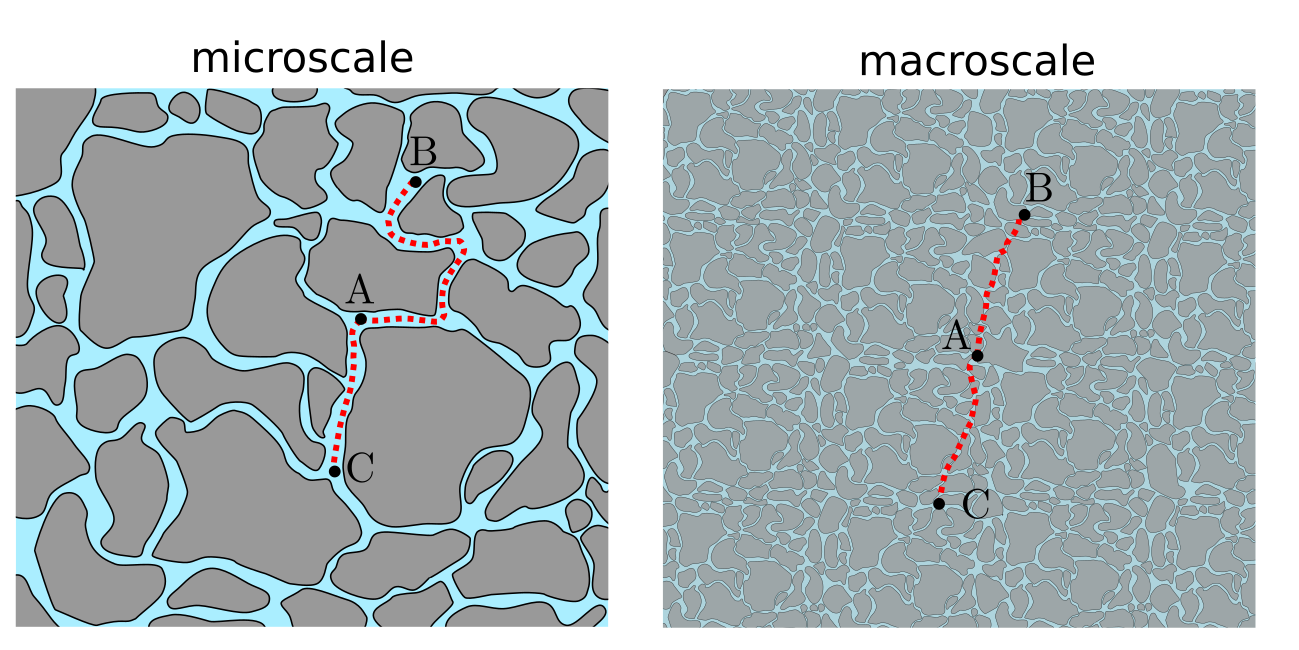
\includegraphics[width=0.6\textwidth]{Figures/Sigma/ecs.png}
\end{center}
\caption[]{\textbf{Illustration of a piece of brain tissue.} Extracellular space (light blue) occupies only about a fraction $\alpha$ of the total tissue volume, and has a highly tortuous structure. The tortuosity, $\lambda$, is defined as the ratio between the shortest pathway between two points in space and the euclidian distance between these two points, and accounts for the fact that ions traveling through the medium do not travel in straight lines, but need to take detours around cellular obstacles.
(A) $\alpha$ and $\lambda$ vary on the microscopic scale. For example, the shortest path (red dotted curve) between locations $r_0$ and $r_1$ is more tortuous than the path between locations $r_0$ and $r_2$. (B) On a larger spatial scale, local inhomogeneities average out, and the tissue can be treated as homogeneous. Typical tissue averages for $\alpha$ and $\lambda$ are 0.2 and 1.6, respectively \cite**{Nicholson1998,Sykova2008}. \ghnote{Omform figur i traad m/ figtekst}
\tvnnote{Legg paa panelmarker, A,B}
}
\label{fig:Sigma:ECS}
\end{figure}

%%%%%%%%%%%%%%%%%%%%%%%%%%%%%%%%
\section{\blue{Continuous, porous medium approximation}}
\label{sec:Sigma:continuous}
\index{Continuous medium}
\index{Porous medium}

%%%%%%%%%%%%%%%%%%%%%%%%%%%%%%%%
When presenting the theory for modeling single neurons (Chapter \ref{chap:Neuron}), we may have given the impression that they are solitary creatures living in a vast extracellular space with long distances to their nearest cell neighbors\tvnnote{Could mention that this mental image also stems from the early staining procedures (Cajal, Golgi, Nansen :-)), where only a small fraction of neurons were actually stained. If all had been stained, it would have been pure black}. \tvntxt{If this had been true, the extracellular conductivity would in practice have been that of saline.} This is far from the truth. A cross-section of a piece of brain tissue shows that it is densely packed with neurons and glial cells (\fref{fig:Sigma:ECS}), and that the extracellular space (colored light blue in the figure) occupies only about 20\% of the the total tissue volume.
\tvntxt{Currents moving through the extracellular medium
are typically assumed to move mostly through the extracellular space, while the cells are effectively non-conducting bodies \cite**{Robinson1968,Nunez2006}.}
\tvntxt{From this, we can already make a first rough estimate of the extracellular conductivity: The extracellular saline has a conductivity of about 1.5~\si{\siemens / \metre}, but only occupies about 20\% of the space, meaning that we might expect the extracellular conductivity to be on the order of 1.5~\si{\siemens / \metre} $\cdot$ 0.2 = 0.3~\si{\siemens / \metre}. This value fits perfectly well with the values typically measured in experiments, although the calculation itself vastly underestimates the complex electrical properties of neural tissue.}

The extracellular space has a highly tortuous \index{Tortuosity} geometry, with an average \tvntxt{extracellular distance between cell membranes of only} about 40-60~nm \cite**{Sykova2008}.
At the micrometer scale, the conductivity \index{Conductivity} $\sigma$ in brain tissue is \tvntxt{therefore} highly non-homogeneous and anisotropic. For example, the conductivity in a certain spatial direction will depend on whether there locally is a free extracellular passage in that direction (high conductivity), or whether this passage is blocked by a nearby membrane (low conductivity) (\fref{fig:Sigma:ECS}{\bf A}). 
%Likewise, also the electric potential $\phi$ will vary greatly over tiny distances, depending on the proximity to neural membranes, especially when approaching the nanometer thick Debye-layers building up the membrane charge \cite**{Pods2013}\tvnnote{Kanskje denne setningen hoerer mer hjemme i VC eller Basics?}.
%When we study extracellular potentials, we are typically not interested in these microscopic variations in $\sigma$ and $\phi$, but rather in the values of these entities when averaged over some spatial volume. Electrodes used to record extracellular potentials typically have sizes ranging from 5 $\mu$m to 125 $\mu$m in diameter \cite**{Viswam2019}, which is larger than the typical diameter of a dendrite ($\sim$ 1 $\mu$m). In practice, the electrodes therefore perform such an averaging, and include contributions from several nearby neurons \tvnnote{Remove last half of sentence? Seems like a different issue to me}. \tvnnote{Tok bort dette, da jeg tenker vi dekker dette et annet sted?}
\tvntxt{At a slightly larger spatial scale, of tens or hundreds of micrometers, it is however reasonable to assume that these micrometer scale inhomogeneities average out (\fref{fig:Sigma:ECS}{\bf B}), and that the brain tissue can be treated as a continuous, porous medium \cite**{Nicholson1981,Gratiy2017}. 
This assumption is further motivation by the lack of any alternative, since we can not in experimental settings know the exact microstructure of the brain.} The VC theory presented in the previous chapter was based on the continuous, porous medium approximation, and thus describes the extracellular dynamics on a spatial resolution larger than at least a few micrometers.

A continuous, porous medium is defined by two key parameters \cite**{Nicholson1981}. The first parameter, $\alpha$, is the fraction of the tissue volume that is extracellular space. The second parameter is $\lambda$, the tortuousity of the extracellular medium \cite**{Nicholson1981}. It is defined as the ratio between the shortest \tvntxt{extracellular} pathway between two points in space and the euclidian distance between these two points, and accounts for the fact that ions traveling through the medium do not travel in straight lines, but need to take detours around cellular obstacles. The parameters $\alpha$ and $\lambda$ can be measured experimentally. Typical values are $\alpha = 0.2$ and $\lambda = 1.6$, although these values vary between brain regions and even locally due to cellular swelling or shrinkage \cite**{Nicholson1998,Sykova2008}.
\tvnnote{Mention that $\alpha$ also varies considerably with brain state, for example with sleep? If I remember correctly, Nagelhus et al (inlcuding Klas) tried to measure brain conductivity to assess brain-state or something like that?}

The continuous, porous medium approximation has implications for how we interpret the various concepts and variables that we use to compute extracellular potentials. In particular, it is important for how we understand the conductivity of the tissue medium. In this chapter, we shall compare three different conductivity measures, and we list them here for clarity and later reference:

\begin{itemize}

\item $\sigma_{saline}$ (S/m) is the conductivity of the saline solution that fills up the extracellular space, and is determined by the ion concentrations in the saline solution (see Section \ref{sec:Sigma:concentrationbased}). Since the brain fortunately contains more than just the extracellular solution, $\sigma_{saline}$ only applies microscopically in the small gaps between neurons, and is not the conductivity of brain tissue as a whole.
\tvntxt{The value of $\sigma_{saline}$ is typically measured to be about 1.5~S/m \cite**{Logothetis2007,Martinsen2008,Miceli2017}.}
\item $\sigma_{e}$ (S/m) is the conductivity of the \textit{extracellular medium} \index{Extracellular medium}, as experienced at a macroscopic (coarse-grained) scale by a current traveling exclusively trough the extracellular part of brain tissue. Importantly, this current does not pass through a 3D volume filled exclusively with the \textit{extracellular solution}, but (i) is confined to move only through a fraction $\alpha$ of the total medium volume, and (ii) must take detours around neural and glial obstacles, as reflected through the tortuousity $\lambda$ \cite**{Nicholson1998,Nunez2006}. The macroscopic $\sigma_{e}$ should theoretically be a factor $\alpha/\lambda^2$ lower than the microscopic $\sigma_{saline}$ (see Section \ref{sec:Sigma:concentrationbased}).

\item $\sigma_t$ (S/m) is the macroscopic (coarse-grained) conductivity of the brain tissue, and is the conductivity as experienced by a macroscopic (coarse-grained) current traveling through the tissue. It is $\sigma_t$ (S/m) that one normally measures experimentally, and it is $\sigma_t$ that is the relevant for use in VC theory. If currents through brain tissue were indeed confined to stay exclusively in the extracellular part of it, $\sigma_t$ should be identical to $\sigma_e$. If currents through brain tissue goes through intracellular pathways in addition to the extracellular ones, we would expect
$\sigma_t$ to be greater than $\sigma_e$ \cite**{Okada1994}.

\end{itemize}




%%%%%%%%%%%%%%%%%%%%%%%%%%%%%%%%
\section{\blue{Anisotropic conductivity}}
\label{sec:Sigma:Anisotropic}
\index{Conductivity!Anisotropic}

%%%%%%%%%%%%%%%%%%%%%%%%%%%%%%%%
\tvntxt{Neural tissue typically has clearly anisotropic geometrical properties, for example, 
the very numerous cortical pyramidal cells tend to be geometrically aligned along the depth direction of cortex.
It makes intuitive sense that this anisotropy could also be reflected in the conductivity, so that the conductivity in the depth direction of cortex could differ from the conductivity  in the perpendicular directions.
In \fref{chap:VC}, we assumed that the tissue conductivity $\sigma_t$ was isotropic, i.e., the same in all the spatial directions, however
this is not always true. For example, in cortex it has been found that the conductivity is about 1.5-fold higher in the depth direction, i.e., for currents running in parallel to the axis of pyramidal cell dendrites \cite**{Goto2010}. The cerebellum has an even more pronounced anisotropic geometrical structure, and the conductivity in the depth direction has been found to be about 3-fold higher than in the perpendicular directions for the anuran cerebellum \cite**{nicholson1975}. Finally, a pronounced anisotropy in the conductivity is typically observed in white matter, because the axons are typically oriented in similar directions by the formation of fiber bundles \cite**{Nicholson1965,Logothetis2007,Bangera2010}. This anisotropy in the conductivity of white matter can in certain cases be as strong as a 10-fold increase in conductivity along the fiber bundle \cite**{Nicholson1965,Bangera2010}.
}

However, the overall effect of the anisotropy on extracellular potentials, at least in cortex, often appears to be quite weak \cite**{Logothetis2007,Ness2015,Miceli2017}, and the approximation that $\sigma_t$ is isotropic often gives good predictions of the potential. See~\fref{fig:Sigma:anisotropy_effect} for an example where a 1.5-fold increase in the conductivity along the axis of the apical dendrite \cite**{Goto2010}, only causes a slightly more squeezed shape of the extracellular potential than the isotropic case \cite**{Ness2015,Miceli2017}. Since extracellular potentials are rather insensitive to modest anisotropies, by far the most common approach is to assume that the extracellular conductivity, at least in cortex, is isotropic.

\begin{figure}[!ht]
\begin{center}
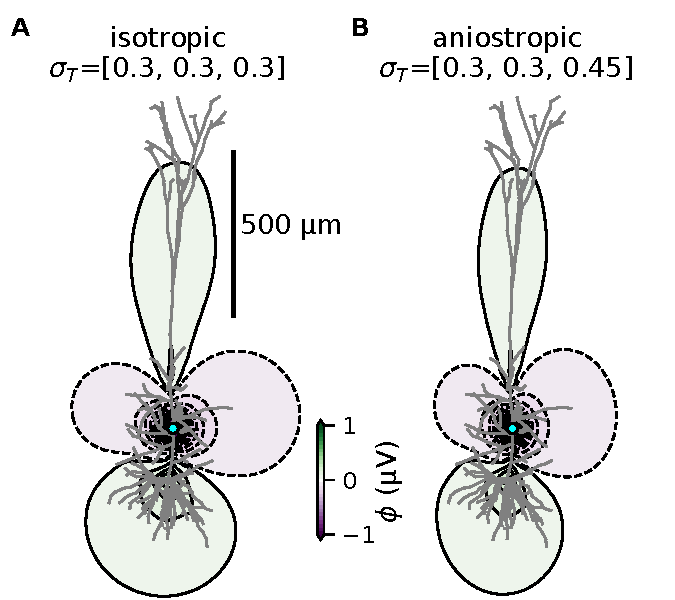
\includegraphics[width=0.6\textwidth]{Figures/Sigma/fig_anisotropy_effect.pdf}
\end{center}
\caption[]{\textbf{Effect of modest anisotropy.}
Extracellular potential at a snapshot in time following a single excitatory synaptic input (location marked by cyan dot) to a rat cortical layer 5 pyramidal neuron \cite**{Hay2011}.
The extracellular potential is shown for the time step corresponding to the maximum observed absolute value for the extracellular potential, and it is calculated from the same neural simulation, at the same time with either an isotropic extracellular medium ({\bf A}) or with an anisotropic extracellular medium, with a 50\% higher
conductivity along the axis of the apical dendrite ({\bf B}). The calculation with anisotropic conductivity was done with \fref{eq:Sigma:Panisos}.
}
\label{fig:Sigma:anisotropy_effect}
\end{figure}

%\tvnnote{Give example already here of where this is particularly relevant?: White matter, Cerebellum, and also mention 50\% increase in cortex, from Goto.}
When deemed necessary, it is relatively straightforward to expand the VC theory to the case of an anistotropic $\sigma_t$. In this case, $\sigma_t$ will no longer be a scalar, but instead a tensor with the three components $\sigma_{tx}$, $\sigma_{ty}$ and $\sigma_{tz}$.
If we use the point source approximation (\fref{eq:VC:pointsources}), the extracellular potential surrounding a set of point current sources $I_k$ is given by \cite**{nicholson1975,Parasnis1986}:

\begin{equation}
\phi(x,y,z) = \sum_k \frac{I_k}{4\pi\sqrt{\sigma_{ty}\sigma_{tz} (x-x_k)^2 + \sigma_{tx}\sigma_{tz} (y-y_k)^2 + \sigma_{tx}\sigma_{ty} (z-z_k)^2}}.
\label{eq:Sigma:Panisos}
\end{equation}
If we use the CSD-description of the sources (eq.~\ref{VC:eq:csds}), the corresponding expression is:
\begin{equation}
\phi(x,y,z) = \iiint_V \frac{C(x,y,z)}{4\pi\sqrt{\sigma_{ty}\sigma_{tz} (x-x_k)^2 + \sigma_{tx}\sigma_{tz} (y-y_k)^2 + \sigma_{tx}\sigma_{ty} (z-z_k)^2}} \, dV.
\label{eq:Sigma:Canisos}
\end{equation}
\tvnnote{Should we derive this in an appendix? It seems it is quite hard to find a derivation of this in the literature, but I managed to find one eventually. (Parasnis1986)}

%\ghnote{Trenger vi en presisering her? Hva betyr det at effekten er lav? Jeg tenker at 50 prosent stoerre sigma burde gi 50 prosent stoerre amplituder, og det er vel ikke en svak effekt? Mener vi at spenningen i en utvalgt retning er relativt upaavirket av anisotropi i andre retninger enn den utvalgte?}
%\tvnnote{La til figur. Vi ble overasket i Ness et al. (2015), over at det nesten ikke var noe synlig effect, hverken naar det var simulert med FEM eller med punktkilde-formlene. Forskjellen kan kanskje kvantifiseres bedre, men er det noe vits?}



%%%%%%%%%%%%%%%%%%%%%%%%%%%%%%%%
\section{\blue{Nonhomogeneous conductivity}}
\label{sec:Sigma:nonhomo}
\index{Conductivity!Nonhomogeneous}
\tvnnote{In- or non-homogeneous?}
In \fref{chap:VC}, we assumed that the extracellular conductivity $\sigma_t$ was homogeneous, i.e., the same everywhere. Clearly, this assumption does not hold on the micrometer scale, where neural tissue is highly non-homogeneous \cite**{Nicholson1998}, see \fref{fig:Sigma:ECS}.
On a very large spatial scale, for example at the scale of whole brains, it is again clear that the tissue is non-homogeneous, since the brains, even for large primates, are not infinite in size.
However, on a mesoscopic spatial scale the microscale inhomogeneities tend to average out (cf. the continuous medium approximation), while the boundaries to other tissue types or materials are often sufficiently distant to have a negligible effect on extracellular potentials. In such cases, for example within a given brain region such as cortex, a homogeneous conductivity appears to be a reasonable approximation \cite**{nicholson1975,Okada1994,Logothetis2007,Goto2010,Ness2015}.

There are however still many scenarios where an infinite homogeneous medium is not a reasonable assumption,
typically because of boundaries between neural tissue and other tissue types or materials.
%For example, for electric potentials measured close to the surface of the brain, the transition from neural tissue  (like for ECoG measurements, see also \ref{chap:ECoG}),
%The situation is different when signals are recorded very far from their sources. It is then likely that they on their journey have experienced a $\sigma_t$ that varied on a macroscopic scale \tvnnote{Er det egentlig riktig aa snakke om "reisen" til et potensial? }.
%For example, electroencephalography (EEG) signals recorded outside of the head are strongly affected by the presence of the brain tissue, cerebrospinal fluid (CSF), skull and scalp, which are very different media with different electrical  conductivities.
When the extracellular medium is non-homogeneous, there is no general analytical formula available (like eqs. \ref{VC:eq:csds}, \ref{eq:Sigma:Panisos} or \ref{eq:Sigma:Canisos}) that link the extracellular potentials to the underlying current sources. In principle, one can however always solve eq. \ref{VC:eq:CSD2} for arbitrarily complex geometries with varying conductivities using numerical methods, like the Finite Element Method (FEM) \cite**{Logg2012}.
This approach has for example been used to model electroencephalography (EEG) signals recorded outside of the head, because these potentials are not only affected by the conductivity of brain tissue, but also by the presence of the cerebrospinal fluid (CSF), skull and scalp, which have widely different conductivities. This is covered in more detail in \fref{chap:EEG}.
Substantial inhomogeneities can also be introduced into neural tissue through the presence of big electrode shanks, as briefly discussed in \fref{sec:VC:elec_shafts}.
%For examples of neuroscience applications using this approach, see \cite**{Moffitt2005,Frey2009,Joucla2012,Haufe2015,Ness2015,Buccino2019b,Obien2019}.

\subsection{Planar boundaries: The cortical surface and {\it in vitro} slice recordings}
For some simple and highly symmetric cases of inhomogeneous volume conductors, analytical solutions can be found for calculating extracellular potentials from the underlying current sources.
An important example of this is (approximately) planar boundaries between different tissue-types or different materials. In such cases, we can use the Method of Images (MoI)\index{Method of Images} from electrostatics \cite**{Jackson1998} to account for the effect of a planar boundary on the extracellular potential from current sources \cite**{Gold2006,Pettersen2006,Nunez2006,Ness2015,Obien2019}. This is done by introducing virtual current sources on the opposite side of the boundary with the same distance to the boundary as the original point current sources, and with the amplitudes scaled by \cite**{Nunez2006,Ness2015},
\begin{equation}
W = \frac{\sigma_1 - \sigma_2}{\sigma_1 + \sigma_2}.
\label{Sigma:eq:MoI_scaling}
\end{equation}
Here, $\sigma_1$ is the conductivity of the region containing the real current sources, and $\sigma_2$ is the conductivity of the region at the other side of the boundary containing the virtual sources.
For example, before inserting recording electrodes into the brain the cortical surface will typically be exposed, and materials of widely different conductivity can be used to cover the cortical surface.
To account for the effect of the different conductivity of cortex and the cover material, the point source equation
(\ref{eq:VC:pointsource2}) must be modified \cite**{Nicholson1971,Pettersen2006},
\begin{equation}
\phi({\bf r}) = \frac{I_k}{4\pi \sigma_t |{\bf r-r_k}|} + \frac{\sigma_t - \sigma_{\rm cover}}{\sigma_t + \sigma_{\rm cover}} \frac{I_k}{4\pi \sigma_t |{\bf r-r_k'}|},
\label{eq:Sigma:MoI}
\end{equation}
where ${\bf r}_k'$ is the location of the virtual current source, mirrored across the cortical surface.
Note that the equation on this form is
only valid within the region with the real source, while other formulas apply outside of this region \cite**{Nunez2006}.
The material at the cortical surface can substantially affect potentials measured near the cortical surface, as illustrated in \fref{fig:Sigma:cortical_surface_effect}.
In particular, notice from \fref{eq:Sigma:MoI} the special case of a measurement performed at the planar boundary to a non-conducting region, so that $|{\bf r-r_k}|=|{\bf r-r_k'}|$, and $\sigma_{\rm cover}=0$. In this case, the measured potential will be exactly a factor of two larger than for an infinite homogeneous medium.

\begin{figure}[!ht]
\begin{center}
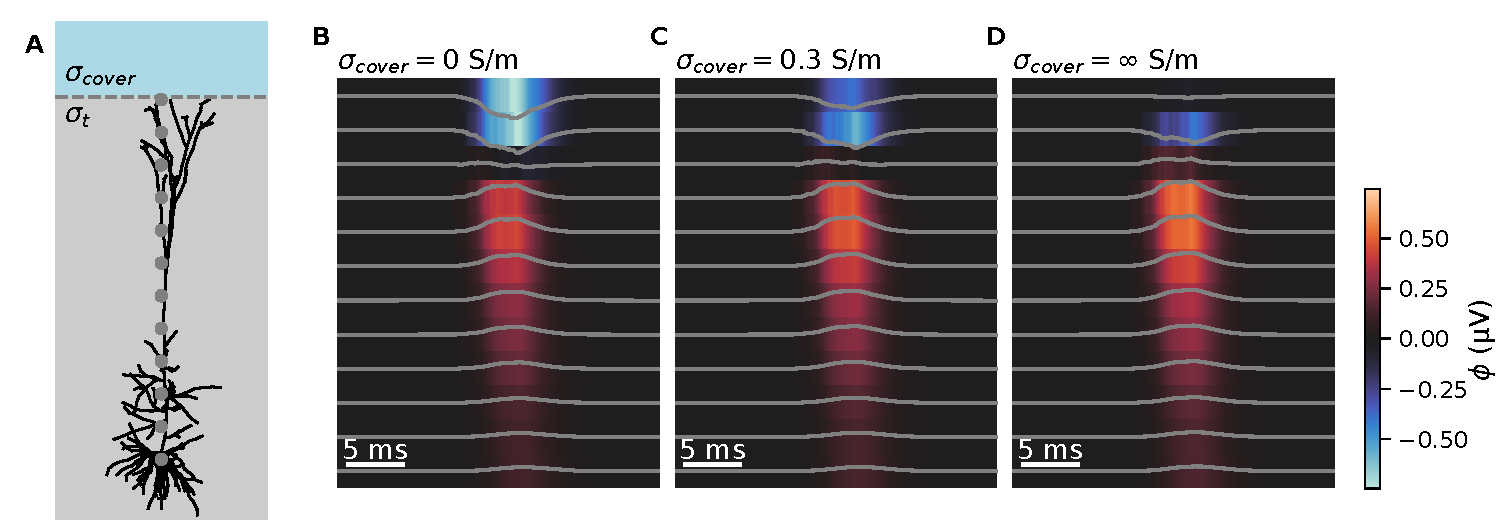
\includegraphics[width=1\textwidth]{Figures/Sigma/fig_cortical_surface_effect_MoI.pdf}
\end{center}
\caption[]{\textbf{Effect of inhomogeneity of cortical surface}
{\bf A:} Simulation set-up. A rat cortical layer 5 pyramidal cell \cite**{Hay2011} receives a wave of excitatory synaptic input to the upper apical dendrite (top 200~$\mu$m). The conductivity of cortical tissue is $\sigma_t$=0.3~S/m, while different conductivities of the region above cortex is tested.
{\bf B:} The cover is an insulator, $\sigma_{\rm cover}$ = 0.0~S/m, like a non-conducting mineral oil or air.
{\bf C:} The cover has the same conductivity as tissue, $\sigma_{\rm cover}$ = 0.3~S/m, corresponding 	to an infinite homogeneous volume conductor.
{\bf D:} The cover is highly conductive, $\sigma_{\rm cover}$ = $\infty$~S/m, like a metal plate.
See also \citeasnoun**{Pettersen2006}.
}
\label{fig:Sigma:cortical_surface_effect}
\end{figure}
%%%%%%%%%%%%%%%%%%%%%%%%%%%%%%%%

The same framework with MoI can also be used to model {\it in vitro} slice recordings, where a small slice of neural tissue is extracted from a brain and placed on a micro-electrode array (MEA), immersed in a saline bath. In this case, there are two planar boundaries, namely the lower boundary between the slice and the non-conducting MEA (glass) electrode plate, and the upper boundary between the slice and the saline bath, see \fref{fig:Sigma:MEA_illustration}.
The two boundaries instead of one gives rise to an infinite series of virtual current sources, which for the simplest case of the measurement being performed at the lower boundary to a non-conducting region, can be written like:
\begin{eqnarray}
\label{eq:Sigma:moi_PS}
\phi(x,y,0) & =  & \frac{2I}{4\pi \sigma_T} \bigg( \psi_{PS}(x,y,z')  \nonumber \\
& + & \sum_{n=1}^{\infty} W_{TS}^n\bigg[ \psi_{PS}(x,y,-z' + 2nh) + \psi_{PS}(x,y,-z' - 2nh) \bigg ]\bigg),
\end{eqnarray}
with 
\begin{equation}
\psi_{PS}(x,y,\tilde z) \equiv \left((x-x')^2 + (y-y')^2 + \tilde z^2)\right)^{-1/2}.
\end{equation}

For an example of this framework, for modelling spikes in {\it in vitro} slices, see \fref{fig:Spikes:MEA-spikes}, and for further details see \citeasnoun**{Ness2015}.
\begin{figure}[!ht]
\begin{center}
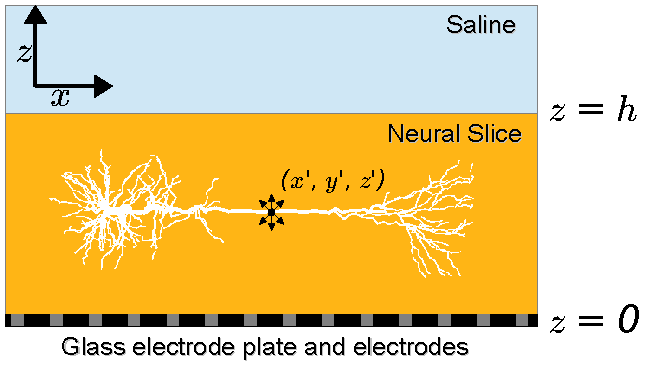
\includegraphics[width=0.4\textwidth]{Figures/Sigma/MEA_illustration.pdf}
\end{center}
\caption[]{\textbf{Illustration of MEA recording set-up.}
See also \citeasnoun**{Ness2015}.
}
\label{fig:Sigma:MEA_illustration}
\end{figure}
%%%%%%%%%%%%%%%%%%%%%%%%%%%%%%%%


\section{\red{Frequency dependence of the conductivity}}
\label{sec:Sigma:f-independent}
\index{Conductivity!Frequency dependence}
%\ghnote{GH: Skrev skisse til dette. Puttet figuren m/ sigma-maalinger inn her, da disse ser ut til aa primaert diskuteres opp mot eventuell frekvensavhengighet. Mulig vi burde ha med "eksperimentelle maalinger i kapittel-tittelen?}

%Regardless of the level of isotropy and homogeneity of a medium, its response to an imposed alternating current can depend on the frequency of the current. Then, the conductivity contains a resistive part, which is real and frequency independent, and an imaginary part that accounts for capacitive and inductive effects that are frequency dependent.
An important question for interpreting and modelling electric signals in neuroscience is whether the conductivity of neural tissue is frequency dependent. If a substantial frequency dependence is present, this would mean that the recorded signals are distorted as they propagate through the medium, and it would bias recordings towards certain parts of the frequency spectrum. In this subsection we will briefly cover the experimental measurements investigating this issue, as well as the theory needed to model such effects, should it be deemed necessary.

We have earlier stated that extracellular currents are typically assumed to move mostly through the extracellular saline solution, where the cells can basically be treated as non-conducting objects (\fref{sec:Sigma:continuous}). If this is true, we would expect the extracellular conductivity to be frequency-independent, since saline is known to be an ohmic medium \cite**{Martinsen2008}. 
A frequency dependence in the extracellular conductivity would however not in itself be surprising: As we have seen, the extracellular space is tightly packed with neurons, and because of the capacitive properties of their membranes, their membrane conductivity is highly frequency dependent (\fref{sec:Neuron:Cap}). Therefore, one could easily imagine that low-frequency extracellular currents are more confined to move resistively through the extracellular space, while
high-frequency extracellular currents could move both resistively through the extracellular space and capacitively through the cells. This would effectively introduce a higher conductivity for higher frequencies, thereby reducing the amplitude of high-frequency extracellular potentials (see \fref{eq:Sigma:pointsource_freq_dep}). This would for example imply that the low-frequency LFP signals are less attenuated than the high-frequency spikes. 
It has been suggested that "stability" of LFP and sensitivity of spikes to position is caused by this, and EEG has "only" low frequencies \cite**{Logothetis2007}, and 1/f power-laws in LFP
\tvnnote{Expand a little on this and cite the French}.

Earlier investigations of the frequency dependence of the extracellular conductivity (also called the impedance spectrum) reported little or no frequency dependence \cite**{Ranck1963,nicholson1975,Pfurtscheller1975}. However, a later study by \citeasnoun**{Gabriel1996} reported a substantial frequency dependence,
in particular below 100~\si{\hertz} (\fref{fig:Sigma:freq_dep}). 
More recent studies again seem to measure little or no frequency dependence of the extracellular conductivity \cite**{Logothetis2007,Elbohouty2013,Wagner2014,Dowrick2015,Miceli2017,Ranta2017,Avery2017}. 
Many of these studies consistently measured an increase of the conductivity of about 20-50\% from a few hertz to some hundreds or thousands of hertz, however, at least in some cases, a similar frequency dependence was also measured in saline, indicating that this frequency dependence at least partially originated in the recording equipment \cite**{Logothetis2007,Miceli2017}. 

\begin{figure}[!ht]
\begin{center}
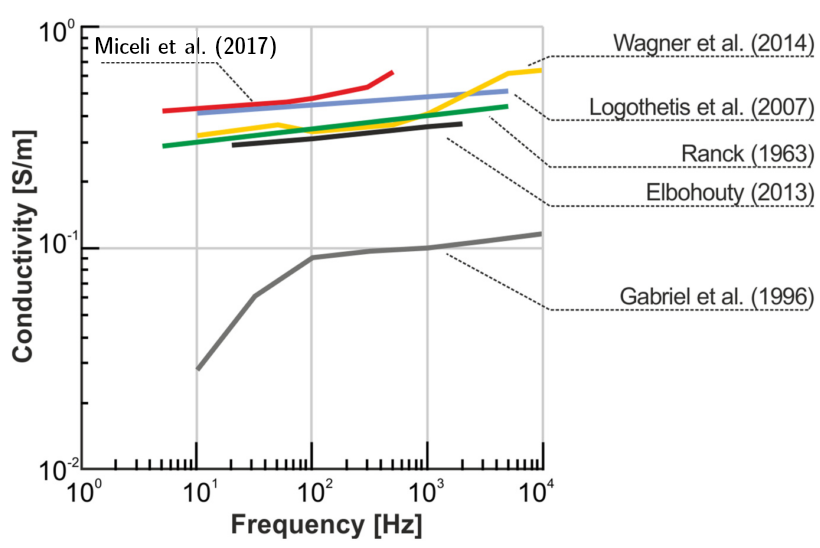
\includegraphics[width=0.6\textwidth]{Figures/Sigma/frequency_dependence.png}
\end{center}
\caption[]{\textbf{Literature review of reported conductivities in various species and experimental setups.}
Most studies seem to indicate a very weak frequency dependence of the extracellular conductivity\index{Conductivity}, which would have a negligible effect on measured extracellular potentials \cite**{Miceli2017}. The very low and strongly frequency dependent values measured by \cite**{Gabriel1996} represents an outlier, and although it has received substantial attention, it has to the best of our knowledge not been reproduced by any other study. For details about the data, see \cite**{Miceli2017}, and references therein \cite**{Ranck1963,Gabriel1996,Logothetis2007,Elbohouty2013,Wagner2014}.
}
\label{fig:Sigma:freq_dep}
\end{figure}

The study by \citeasnoun**{Gabriel1996} clearly stands out, as it is the only study to our knowledge to experimentally measure a strong frequency dependence for low frequencies. This study also reported a conductivity of only about 0.03~\si{\siemens/ \metre} at 10~\si{\hertz}, about an order of magnitude lower than the commonly reported values. This value seems surprisingly low, given that healthy neural tissue contains a substantial fraction of highly conducting saline.
 The authors were however careful to note that the reported low-frequency values might be distorted by inadequate correction for electrode polarization (see \fref{sec:VC:electrodes} 
 for a brief review of electrode polarization). Further, a later study using the same recording equipment did not observe a similarly strong frequency-dependence, or similarly low conductivity values (\citeasnoun**{Wagner2014}; \fref{fig:Sigma:freq_dep}). Finally, their recording were done in bovine brains obtained from a slaughterhouse up to a couple of hours post-mortem \cite**{Gabriel1996}, which can potentially have resulted in suboptimal tissue preservation and cell swelling. 

Consequently, experimental data is consistent with neural tissue being ohmic, or with having at most a weak frequency dependency of the order of up to $\sim$30\% over the frequency range of interest for neurophysiology (below a few thousand hertz). This might not sound very small, but modelling studies of frequency dependencies of this order has indicated that it would have a relatively minor effect on measured potentials \cite**{Bossetti2008,Tracey2011,Miceli2017}\tvnnote{Add figure adapted from Miceli2017?}. Note however that this is not necessarily true for extracellular current stimulation with very brief current pulsed, because of the very high frequency content of the pulses (\fref{chap:Stim}; \citeasnoun**{Bossetti2008}).

For a frequency-dependent conductivity, the point-source equation becomes \cite**{plonsey1967,Bossetti2008,Miceli2017}:
\begin{equation}
\phi({\bf r}, \omega) = \frac{I(\omega)}{4\pi (\sigma_t(\omega) + {\rm j} \omega \epsilon(\omega)) r},
\label{eq:Sigma:pointsource_freq_dep}
\end{equation}
\tvnnote{notation must be fixed}
Note that while both $\sigma_t(\omega)$ and $\epsilon(\omega)$ can be frequency dependent, they are not independent: To obey causality, that is, that the extracellular potential originating from a current can not precede the current, there must be a certain relationship between $\sigma_t(\omega)$ and $\epsilon(\omega)$, which can be found from the Kramers-Kronig relation, or equivalently from the Bode relation between the magnitude of the conductivity $|\sigma(\omega)|$ and the induced phase-shift $\exp ^{-{\bf j} \theta(f)}$.

%In Section \ref{chap:VC:onlyohmic}) we argued that the extracellular displacement current is negligible, which means that the extracellular medium in itself (and thus $\sigma_e$) does not exhibit any capacitive effects. This alone does not rule out the possibility that the effective conductivity of the tissue medium ($\sigma_t$) includes capacitive effects, as currents traveling through it could interact with nearby capacitive neural membranes.

%However, for the relevant frequencies in extracellular recordings (\fref{fig:Sigma:freq_dep}), the capacitive and inductive effects appear to be negligible compared to the resistive effects \cite**{Logothetis2007,Miceli2017,Ranta2017}. In most applications of VC theory, one therefore applies the assumption that the medium is Ohmic or resistive, meaning that the imaginary and frequency dependent part of the conductivity is zero. We note, however, that it is possible to expand the formalism to include a frequency dependent conductivity \cite**{Bedard2004,Tracey2011,Miceli2017}.

%\tvnnote{Utledning tilsvarende Appendix B i Nunez?}
%\ghnote{Vet ikke helt.... Appendixet gir et greit bevis paa at kapasitive effekter i ECS er smaa. De foelger opp med et tilsvarende studium av membranen, men i det studiet er det membranen alene som er mediumet. Saa vidt jeg kan se faar vi ingen pekepinn paa hva membranens tilstedevaerelse gjoer for tissue-stroemmer....}


%\begin{figure}[!ht]
%\begin{center}
%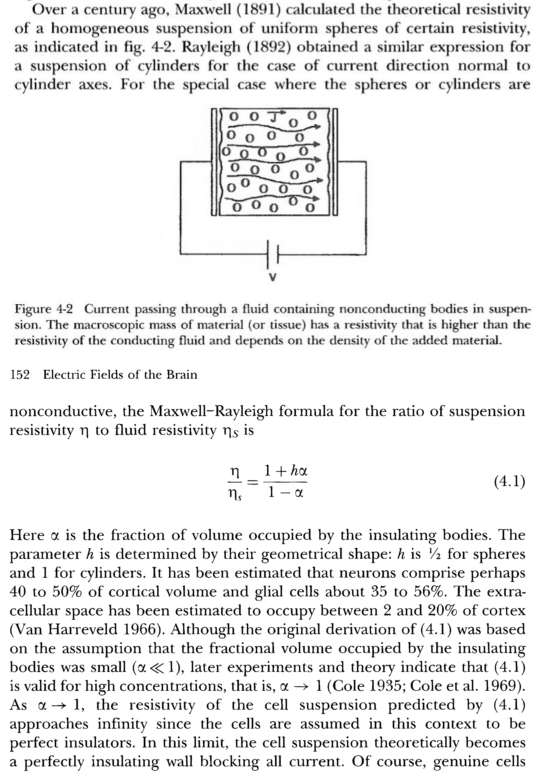
\includegraphics[width=0.6\textwidth]{Figures/Sigma/resistivity_maxwell.png}
%\end{center}
%\caption{\textbf{From Nunez} \tvnnote{Ta med noe slikt?}}
%\label{Sigma:fig:maxwell_resistivity}
%\end{figure}

\section{\red{TVN: Theoretical explorations....} }
\index{Conductivity!Theoretical estimates}

\ghnote{Dette var et punkt i den opprinnelige planen. Referenser: Meffin2012,
Tahayori2012, Meffin2014, Tahayori2014. Jeg vet ikke helt hva dette gaar i, men det gjoer sikkert Torbjorn og/eller Gaute?}


\section{\blue{GH: Theoretical estimate of the conductivity based on ion concentrations} }
\label{sec:Sigma:concentrationbased}
\index{Conductivity!Ion concentration dependence}

Extracellular current are mediated by the ions dissolved in the extracellular solution, and the conductivity of the extracellular medium if thus a function of thus depends on the ion concentrations, i.e., on the availability of free charge carriers \cite**{Grodzinsky2011}:

\begin{equation}
\sigma_{saline} = \frac{F^2}{RT}\sum_{k} D_k z_{k}^2 c_{k}.
\label{Sigma:eq:sigma1}
\end{equation}
Here $z_{k}$, $D_k$ and $c_{k}$ denote the valency, diffusion coefficient and concentration, respectively, of ion species $k$, while $F = 96485.3$ C/mol is the Faraday constant, $R = 8.314$ JK$^{-1}$mol$^{-1}$ is the gas constant, and $T$ the temperature.

Eq. \ref{Sigma:eq:sigma1} allows us to compare the measured $\sigma_t$ with $\sigma_{saline}$ as predicted from the typical ion concentrations in the extracellular space of the brain, such as those listed previously in Table \ref{Neuron:tab:ion-concentrations}. For this, we also need the diffusion constants of these species. In a dilute solution, such as the extracellular fluid, these are as given in Table \ref{Sigma:tab:diffconsts}.

\begin{table}[h!]
\begin{center}
\caption[Diffusion Constants]{Diffusion constants. Values taken from from \cite**{Bowen2002,Lyshevski2007}}
\label{Sigma:tab:diffconsts}
    \begin{tabular}{l|l}
    \hline
    $D_{Na}$ & $1.33\times 10^{-9}$ m$^2$/s\\ \hline
    $D_K$ & $1.96  \times 10^{-9}$ m$^2$/s \\ \hline
    $D_{Cl}$ & $2.03 \times 10^{-9}$ m$^2$/s \\ \hline
    $D_{Ca}$ & $0.71\times 10^{-9}$ m$^2$/s \\ \hline
    $D_{Mg}$ & $0.72\times 10^{-9}$ m$^2$/s \\ \hline
    $D_{HCO3}$ & $1.18\times 10^{-9}$ m$^2$/s \\ \hline
    \end{tabular}
\end{center}
\end{table}

If we insert the values from Tables \ref{Neuron:tab:ion-concentrations} and \ref{Sigma:tab:diffconsts} into equation \ref{Sigma:eq:sigma1}, and assume a body temperature of $T = 310$ K, we get a conductivity $\sigma_{saline} = 1.72$ S/m. This is a factor 6-9 times higher than the values (0.2-0.3 S/m) which are typically measured for the tissue conductivity.

Currents through brain tissue do not move through a pure ion solution, and the effective tissue conductivity $\sigma_t$ is lower than $\sigma_{saline}$ for two main reasons. Firstly, extracellular currents are confined to stay in the small fraction $\alpha$ of the tissue volume that is extracellular, so that only a fraction $\alpha$ of the tissue volume has the conductivity predicted by eq. \ref{Sigma:eq:sigma1}. Secondly, even within the extracellular volume fraction, eq. \ref{Sigma:eq:sigma1} overestimates the conductivity, because extracellular currents will encounter obstacles (neural and glial membranes) along their path, forcing them take detours that can be quantified through a tortuosity factor $\lambda$.

If we correct eq. \ref{Sigma:eq:sigma1} for the extracellular volume fraction and tortuous structure of the extracellular space, we get an estimate for the effective tissue conductivity as \cite**{Okada1994}:
\begin{equation}
\sigma_{t} = \frac{\alpha}{\lambda^2} \sigma_{saline}.
\label{Sigma:eq:sigmat}
\end{equation}
Typical values for $\alpha$ and $\lambda$ for the extracellular space of brain tissue are 0.2 and 1.6, respectively \cite**{Nicholson1981,Nicholson1998}. With these values, $\sigma_t$ becomes almost a factor 13 lower than $\sigma_{saline}$.

With our above estimate of $\sigma_{saline}$, we get a an estimated tissue conductivity $\sigma_t = 0.134$ S/m. This is lower than the typical measured values for $\sigma_t$, which, although they vary quite much between different experiments, tend to be $> 0.2$ S/m. The main explanation to why our $\sigma_t$ is an underestimate is probably that it is based on the assumption that all tissue currents are confined to the extracellular space, while a fraction of the real tissue currents may also travel through the intracellular medium. For example, in cerebellum, it has been estimated that about 50 \% of tissue currents travel through intracellular paths \cite**{Okada1994}. An additional explanation is that the extracellular solution contains many ions (such as e.g., H$^+$ and HPO4$^{2-}$ ) that we did not include in Table \ref{Neuron:tab:ion-concentrations} and thus not in our calculation of $\sigma_t$. However, since concentrations of ions others than those in Table \ref{Neuron:tab:ion-concentrations} are quite low, they will probably have only a minor impact on the conductivity.

As we shall see in Chapter \ref{sec:Eldiff}, the definition of $\sigma_t$ given by eq. \ref{Sigma:eq:sigmat} follows naturally if we use the Nernst-Planck equation for electrodiffusive ion concentration dynamics to compute extracellular currents.

\chapter{\ehtxt{Numerical} schemes for computing extracellular potentials}
\label{sec:LFPy}
\ghnote{Torbjorn/Espen will write most this.}
\ghnote{La inn forslag til intro her:}

%%%%%%%%%%%%%%%%%%%%%%%%%%%%%%%%%%%%%%%%%%%%%

The \ehtxt{established \sout{standard}} way of computing extracellular potentials is to use a two-step multicompartment + volume conduction (MC+VC) scheme,
which can be summarized as:

\begin{itemize}
\item {\bf Step 1:} Compute the electrical activity of neurons using a the multicompartment (MC) framework presented in \Fref{chap:Neuron}, assuming that it is unaffected by whatever goes on in the extracellular space.
\item {\bf Step 2:} Compute the extracellular potential $\phi$ resulting from the neural transmembrane currents computed in step 1, using Volume Conductor (VC) theory (Chapters \Fref{chap:VC}-\ref{chap:Sigma}). 
\end{itemize}

The MC+VC scheme is not self-consistent, since Step 1 computes the neurodynamics under the assumption that $\phi$ is \ehtxt{unaffected by transmembrane currents \sout{zero (grounded extracellular space)}},
and Step 2 uses this neurodynamics to compute a non-zero extracellular potential.
\ehnote{I wonder if we should elaborate more on pt. 1: It is entirely possible to impose potentials different from zero and time varying with the current scheme and simultaneously estimate transmembrane currents. The main problem is that cable theory is 1D while real neurons are 3D (with the exception of structures such as axonal tracts).
Self-ephaptic effects should be entirely possible to account for using standard methods (NEURON) for cable models with 1D geometry (at least that's what I think!).}
There exist more complete and consistent schemes that account for both the ephaptic effects from $\phi$ on neurodynamics as well as for effects of ion concentration dynamics on neuronal activity of extracelluar potentials. In general, these more complete schemes require numerical simulations of both the neural and extracellular dynamics using finite element or finite difference methods, and are very computationally expensive.

In most scenarios, ephaptic effects from extracellular potentials on neurodynamics are small, and ion concentrations tend to stay close to baseline. When this is true, the simplifying approximations applied in the two-step scheme do not critically affect the accuracy of its predictions. As the MC+VC scheme is far more computationally efficient than any of the more complete schemes, it remains the gold standard for computing $\phi$ in large population models of neurons mimicking physiologically realistic scenarios. Also, designated software has been developed that makes it easy to perform simulations using the two-step-procedure. Therefore, the simulations in the application part of this book (Part 2) will predominantly be based on on the MC+VC-framework.

When aiming to make realistic simulations of extracellular potentials, one might need to simulate large networks containing thousands of neurons. This is computationally demanding, even on an efficient scheme like MC+VC.
\ehnote{Computational demands are linearly dependent on the total number of compartments, so this a "simple" problem to solve, just scale up your computer capability accordingly.}
As we showed in \Fref{chap:VC},
VC theory gave us \ehtxt{linear} analytical expression\ehtxt{s} for $\phi$ as a direct function of the neural current sources (Step 2), meaning that it is \ehtxt{usually} the simulations of the neurodynamics (Step 1) which is the bottleneck in the simulation. Below, we present computational schemes for the standard MC+VC approach, based on multicompartment neural models (Section \ref{sec:Schemes:LFPy}), and follow up with two strategies that may be applied to reduce the computational cost when computing the neurodynamics (Sections \ref{sec:Schemes:HybridLFPy}-\ref{sec:Schemes:KernelLFPy}). We end the chapter with a brief introduction of an alternative, and self-consistent framework (Section \ref{sec:VC:EMI}).

\ehnote{For meg gir det mer mening og organisere dette i reduksjonistisk rekkefoelge: (1) self-consistent; (2) MC+VC; (3) point-neuron spiking + MC + VC; (4) firing-rate + MC + VC.
Men uansett, burde ikke dette vaere del av "Applications"-kapitlet? Punkt 3 og 4 endrer i prinsippet ingenting med MV+VC formalismen - man disassosierer bare simulering av nettverksaktivitet (korrelasjoner) fra (MC+VC)-formalismen.}



%%%%%%

\section{\ehnote{}\ehtxt{Forward-model predictions from multicompartment neuron models}}
\label{sec:Schemes:LFPy}
\index{Multicompartment models}


Most models aiming to mimic the dynamics of a particular neuron or neural system except the simplest ball and stick like models are too complex to be solved analytically (cf. \Fref{chap:Neuron}).
Thus the set of partial differential equations (PDEs) and initial conditions representing voltage- and concentration-dependent ion channels, synapses, plasticity, neuronal geometry etc. of the full model will have to be solved numerically on computers.
The numerical solution of geometrically detailed cable models entails a discretization of the geometry into multiple compartments (hence MC) wherein the states of variables and their derivatives are estimated on a temporal grid which may be fixed or irregular.
While one could utilize general-purpose numerical solvers in order to compute resulting voltage fluctuations, transmembrane currents or axial currents,
a more feasible approach is utilization of one of several different software tools tailored for this purpose that have been developed in the past.
Such software greatly simplify the process of specifying the phenomenological or biophysically detailed model and choosing the appropriate numerical schemes for solving the resulting set of PDEs.
Such tools will also by default usually account for one of the main assumptions of standard cable theory, that is,
the spatial variation in membrane voltage across the entire morphology can be computed independently of any effect
transmembrane currents may have on the extracellular potential immediately outside the compartments (see chapter \Fref{chap:Neuron} for details).


The NEURON simulation environment\footnote{\href{https://neuron.yale.edu}{https://neuron.yale.edu}} \cite**{Hines1997} presently remains a prevalent choice for empiric-based simulations of MC neuron models as it supports both Windows-,
linux- and unix-based operating systems including MacOS,
and can be used with a GUI or in a programmatic fashion on laptops, desktop computers and in parallel on large-scale high-performance computing (HPC) facilities.
NEURON is also utilized as a simulator backend for other higher-level software such as
PyNN\footnote{\href{https://neuralensemble.org/PyNN/}{https://neuralensemble.org/PyNN/}} \cite**{Davison2008},
NetPyne\footnote{\href{http://www.netpyne.org}{http://www.netpyne.org}} \cite**{Dura_Bernal_2019},
BMTK\footnote{\href{https://alleninstitute.github.io/bmtk/}{https://alleninstitute.github.io/bmtk/}} \cite**{Dai2020},
LFPy\footnote{\href{https://lfpy.readthedocs.io}{https://lfpy.readthedocs.io}} \cite**{Linden2014,Hagen2018} etc.
Alternatives to NEURON with partially overlapping feature sets have been developed in the past in form of
MOOSE\footnote{\href{https://moose.ncbs.res.in}{https://moose.ncbs.res.in}} \cite**{Bhalla2008} and
GENESIS\footnote{\href{http://genesis-sim.org}{http://genesis-sim.org}} \cite**{Bower1998},
while software tailored for point-like neuron models such as
Brian\footnote{\href{https://briansimulator.org/}{https://briansimulator.org/}} \cite**{Stimberg2019} recently received support for biophysically detailed MC neuron models.
Another effort receiving funding from the EU Human Brain Project,
named Arbor\footnote{\href{https://arbor.readthedocs.io}{https://arbor.readthedocs.io}} \cite**{Akar2019},
aims to develop MC neuron simulation software from the ground up in order to fully exploit modern high-performance libraries and next generation hardware in the form of graphical processing units (GPUs) and massively parallel HPC facilities.


\subsubsection{Predicting axial and transmembrane currents}
\label{chap:LFPy_Ia_Im}

Here we will refrain from going into details on the inner workings of the above software tools,
but reiterate that both axial currents and transmembrane currents can be estimated if the set of PDEs can be solved numerically for the membrane voltage of the MC neuron model(s).
The membrane voltages of MC neuron models are typically assumed to be `measured' at the center of each compartment.
The axial and transmembrane currents of a non-branching piece of cable is given in continuous form by
%
\begin{eqnarray}
I_\mathrm{a}(x,t) &=& - \frac{1}{r_\mathrm{i}} \frac{\partial V_\mathrm{m}(x, t)}{\partial x} \text{~and} \\
i_\mathrm{m}(x, t) &=& - \frac{\partial I_\mathrm{a} (x, t)}{\partial x} = \frac{1}{r_\mathrm{i}} \frac{\partial^2 V_\mathrm{m}(x,t)}{\partial x^2}~,
\label{eq:LFPy_ia_im_continuous}
\end{eqnarray}
%
where the intracellular resistance per unit length $r_\mathrm{i}=4R_\mathrm{a}/\pi d^2$ can be given with unit \si{\ohm/\metre}.
Here, $R_\mathrm{a}$  and $d$ is the axial resistivity (\si{\ohm\metre}) and diameter (\si{\metre}) of the dendritic cable model, respectively (cf. \Fref{chap:Neuron}).
The unit for axial currents $I_\mathrm{a}(x, t)$ is \si{\ampere},
while the transmembrane current is per unit length (\si{\ampere/\metre}).
The location $x$ denotes the position along the piece of cable in one dimension (the cable equation is by definition 1D even if the different parts of a neuron may be assigned locations in 3D space).

For spatially discretized cable models the axial currents can be estimated per-compartment by the central difference approximation as
%
\begin{eqnarray}
I_\mathrm{a}(x_j, t) &\overset{h>0}{\approx}& - \frac{1}{r_\mathrm{i}} \frac{V_\mathrm{m}(x_j+\frac{h}{2}, t) - V_\mathrm{m}(x_j-\frac{h}{2}, t)}{h} \nonumber \\
		  &\overset{L_j=h}{=}& - \frac{\pi d_j^2}{4 R_\mathrm{a}} \frac{V(x_j - \frac{L_j}{2}, t) - V_\mathrm{m}(x + \frac{L_j}{2}, t)}{L_j} ~.
\label{eq:LFPy_ia_discrete}
\end{eqnarray}
%
Here, $x_j$ denotes midpoint location,
and the discretization constant $h$ is set equal to the compartment length $L_j$.
Its diameter is typically assumed to be constant,
and the cylindrical compartment is a straight along its length axis.
\ehnote{True for NEURON, but not for Arbor which adapts a FDM type scheme in 1D corresponding to electric compartments made up by series of conical frusta.}
Note that it is possible to swap the central difference approximation
by the forward and  backward difference approximation estimating axial currents for each half-compartment respectively as in \cite**{Hagen2018},
but we will not go into further detail here.

We next outline how the membrane potential can be estimated at the end points of each compartment $x \in \{x_j-L_j/2, x_j+L_j/2\}$,
which may connected to none, one or several other end points of other compartments,
when the neural simulation software returns the midpoint potential $V_\mathrm{m}(x_j, t)$ for every $j \in \{1, \cdots, N \}$ compartment.
For terminating compartments (i.e., one or both ends has no connecting compartments and sealed ends) we may define
%
\begin{eqnarray}
V_\mathrm{m}(x_j - L_j/2, t) &\equiv& V_\mathrm{m}(x_j, t)~\mathrm{and/or} \nonumber \\
V_\mathrm{m}(x_j + L_j/2, t) &\equiv& V_\mathrm{m}(x_j, t)~, \nonumber
\end{eqnarray}
%
depending on which end(s) has no electric connections.
(This step effectively utilize the forward/backward difference approximation to first derivatives but only to terminating compartments.
If both ends terminate, the axial current will be zero as the voltage is implicitly assumed to be iso-potential along the compartment axis.)

For a number $N$ child compartments connected at the end point location $(x_j+L_j/2)$ of the parent compartment (\Fref{fig:LFPy_circuits}C) the potential can be computed from the parent- and child-compartment mid-point potentials as \cite**{Hagen2018}

\begin{equation}
V_\mathrm{m}(x_j+L_j/2, t) = \frac{\sum_{n=0}^N V_\mathrm{m}(x_{j+n}, t) / R_{j+n}}{\sum_{n=0}^N 1 / R_{j+n}}~,
\label{eq:LFPy_V_connect_point}
\end{equation}
%
where the connecting node to mid point resistances
%
\begin{eqnarray}
R_{j+n} &=& \frac{2 R_\mathrm{a}L_{j+n}}{\pi d_{j+n}^2} ~.
\end{eqnarray}

For child compartments connecting to the mid point of the parent compartment,
the corresponding potential at the branch point seen by any number of child segments is per definition the same as the mid point potential of the parent, that is,
\begin{equation}
V_\mathrm{m}(x_{j+n}-L_{j+n} / 2, t) \equiv V_\mathrm{m}(x_j, t) ~.
\end{equation}

Up to this point, we have provided the basic `machinery' needed in order to compute the discrete axial currents in a MC neuron model,
independently of specific and non-specific ion-channel currents, synaptic currents, capacitive currents etc. which may be present in the membrane of biophysically detailed MC neuron models.
By our application of the central difference approximation to the first derivative,
it is in these derivations then implicitly assumed that the axial current is approximately constant along the entire length of the compartment,
which in turn imply that the the membrane voltage varies approximately linearly with position.
The naive computational neuroscientist should remind her/himself that this assumption is likely to be violated if the spatial discretization chosen for the model neuron(s) is too coarse.
%
Also the transmembrane currents may be estimated on a per-compartment basis in a similar manner using the central difference approximation to the 2nd derivative as
%
\begin{eqnarray}
i_\mathrm{m}(x_j, t) &\overset{h>0}{\approx}& \frac{1}{r_\mathrm{i}} \frac{V_\mathrm{m}(x_j + \frac{h}{2}, t) - V_\mathrm{m}(x_j, t)+ V_\mathrm{m}(x_j - \frac{h}{2}, t)}{h^2 / 4} \nonumber \\
		&\overset{L_j=h}{=}& \frac{\pi d_j^2}{R_\mathrm{a}} \frac{V_\mathrm{m}(x_j + \frac{L_j}{2}, t) - V_\mathrm{m}(x_j, t) + V_\mathrm{m}(x_j - \frac{L_j}{2}, t)}{L_j^2} ~.
\label{eq:LFPy_im_discrete}
\end{eqnarray}


This machinery may appear as a bit of a hurdle to implement for the purpose of computing extracellular potentials or magnetic signals,
but thankfully MC neuron modeling software such as NEURON and Arbor provides native support for computing the transmembrane current (\si{\ampere}) and/or transmembrane current density per surface membrane area (\si{\ampere/\metre^2}) for each compartment.
Dependent on the implementation in the neural simulation software,
a more direct measure of the transmembrane currents is indeed computing the sum over all capacitive currents, specific and non-specific ion-channel currents, synapse currents etc. (cf. \Fref{chap:Neuron}).
%
The current state is however a bit more dire with regards to predicting axial current per compartment (or half-compartment \cite**{Hagen2018}).
For now, we will emphasize that typical extracellular measures of extracellular electric or even magnetic signals can be derived from the transmembrane currents alone.

\begin{figure}[!ht]
\begin{center}
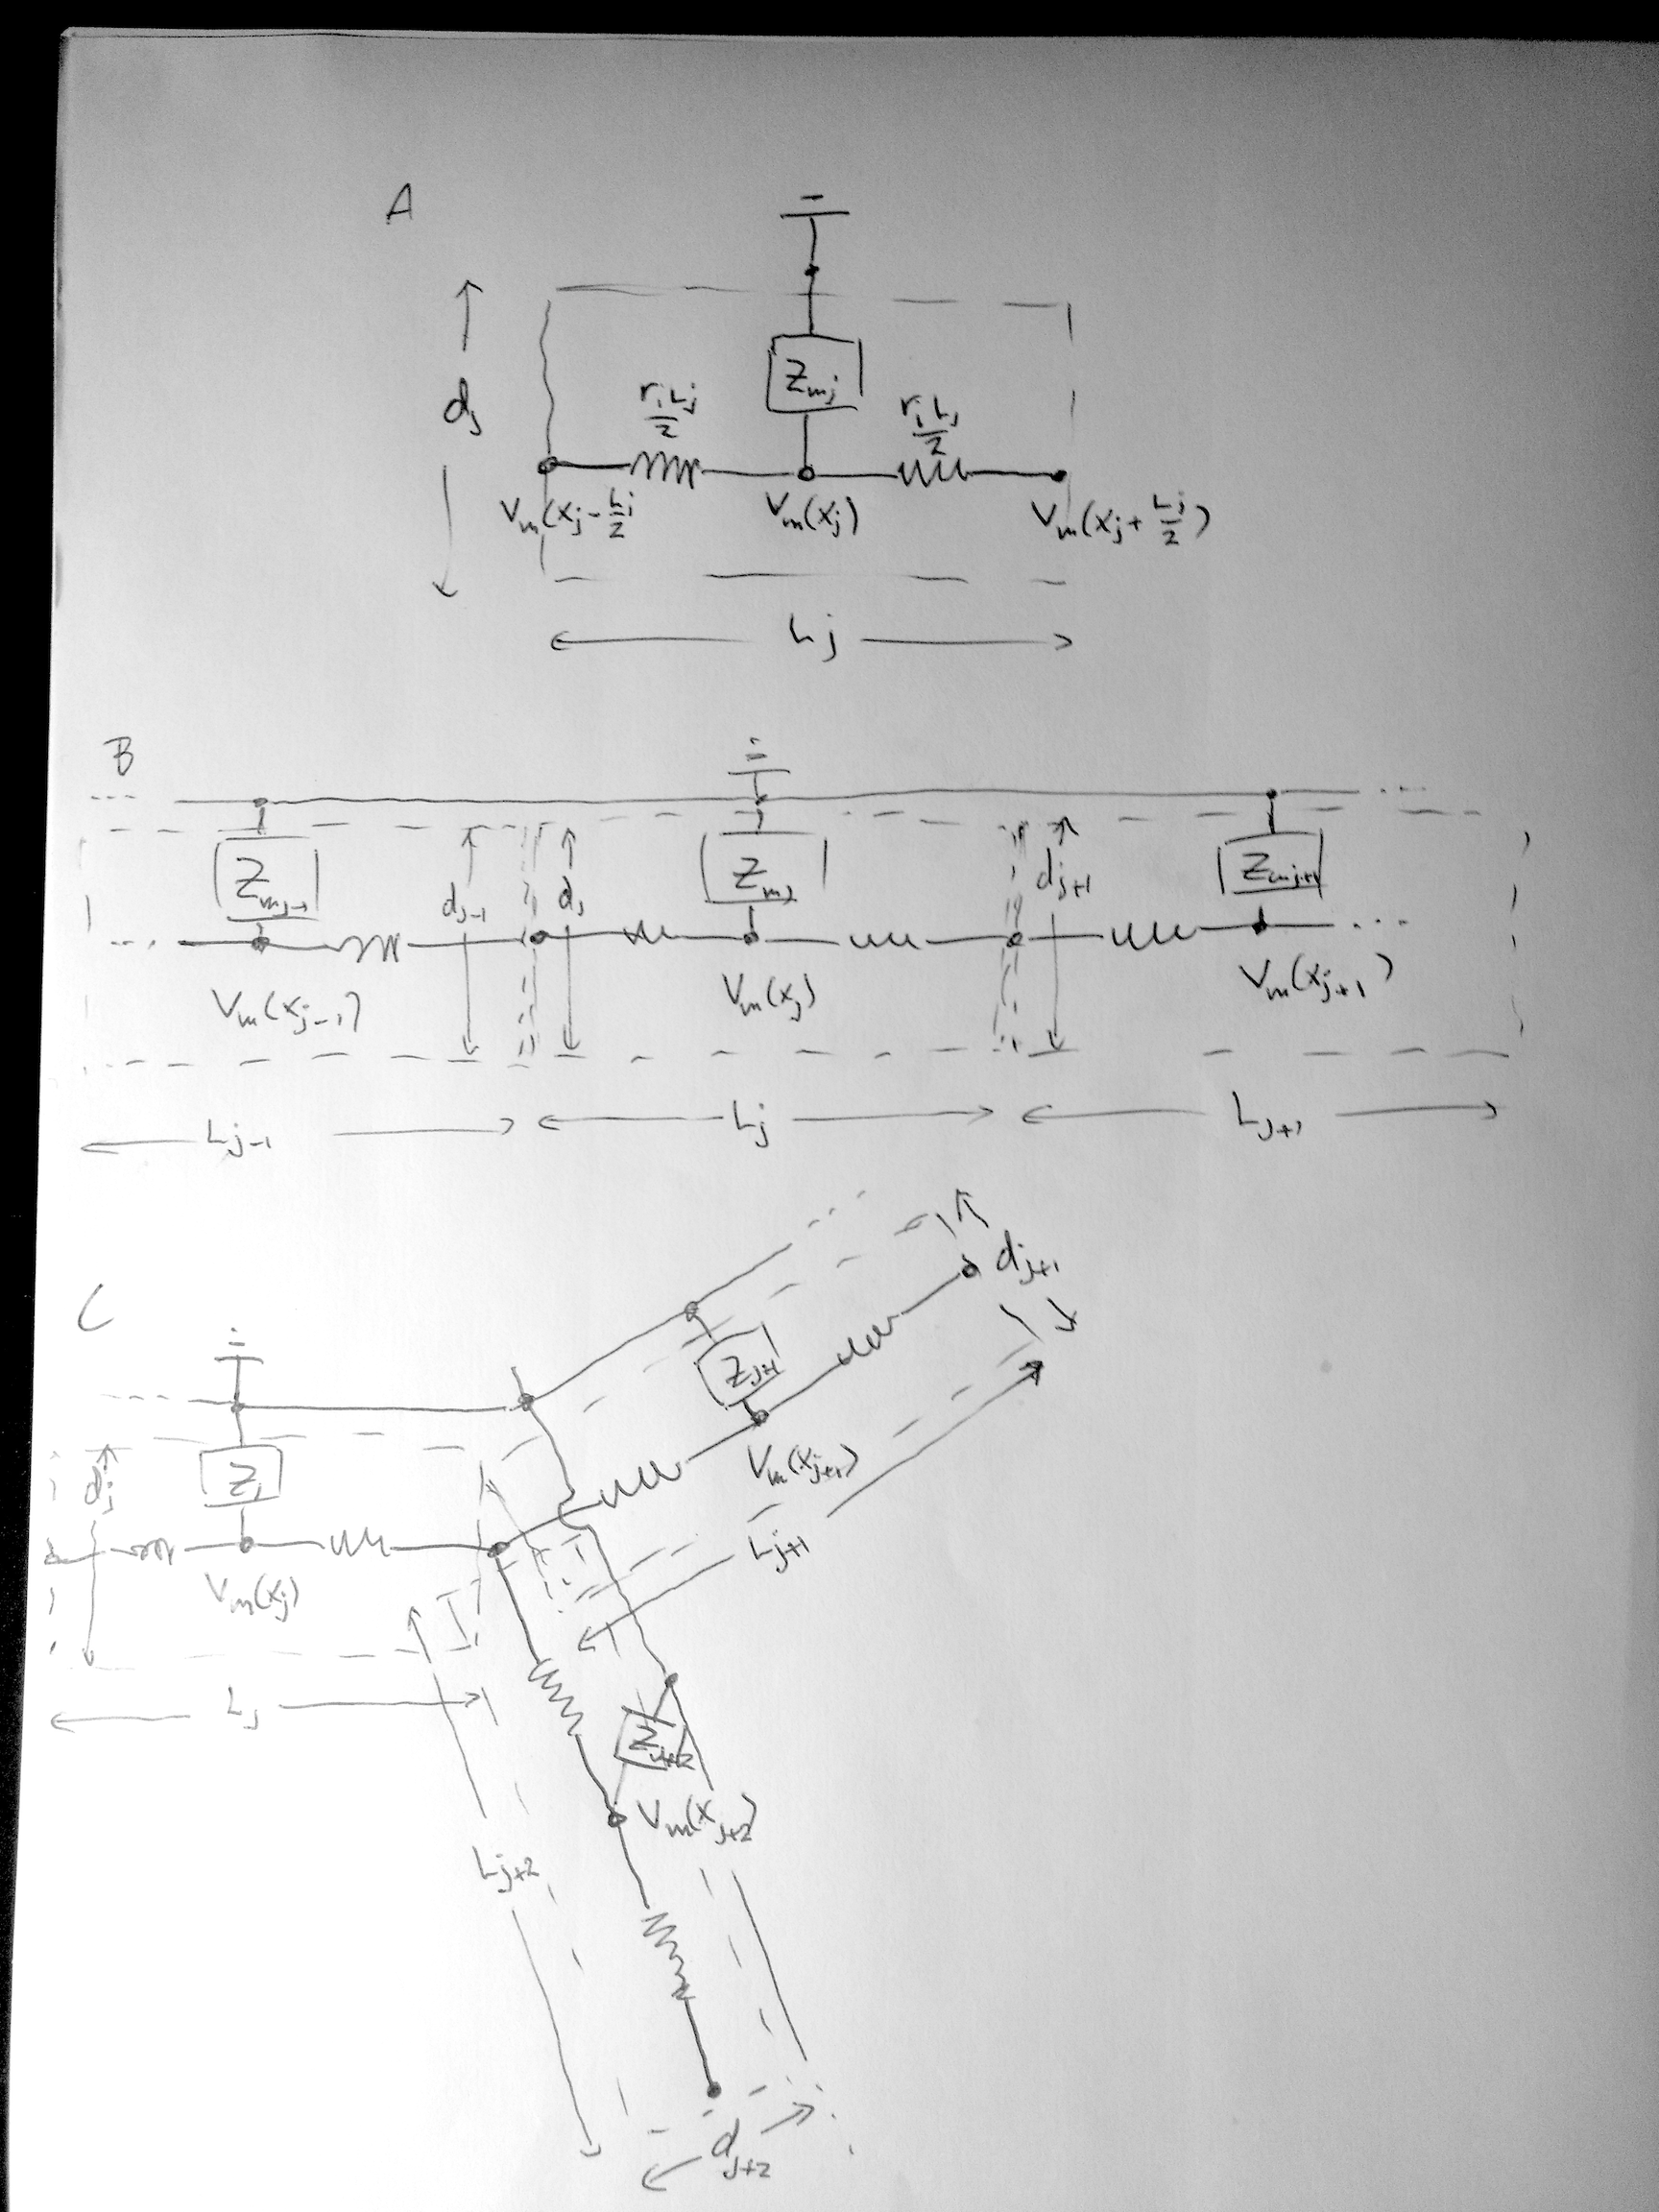
\includegraphics[width=0.8\textwidth]{Figures/Ch-LFPy/circuits.png}
\end{center}
\caption{\textbf{Equivalent circuits for computing axial and transmembrane currents}.
({\bf A}) One-compartment cable model with sealed ends.
({\bf B}) Continuous piece of MC cable model.
({\bf C}) MC cable model with branch point.}
\label{fig:LFPy_circuits}
\end{figure}


Up to this point, the attentive reader of this chapter may have noticed that the axial currents (and transmembrane currents for that matter) is \textit{linearly} dependent on the midpoint membrane voltages of the MC model.
Thus, the full set of operations involved in computing the full set of axial current magnitudes can be rewritten as a linear combination on the form
%
\begin{eqnarray}
\begin{bmatrix}
I_\mathrm{a}(\mathbf{r}_1, t)\\
I_\mathrm{a}(\mathbf{r}_2, t)\\
\vdots \\
I_\mathrm{a}(\mathbf{r}_N, t)
\end{bmatrix}
&=& \mathbf{A}^{-1}
\begin{bmatrix}
V_\mathrm{m}(\mathbf{r}_1, t)\\
V_\mathrm{m}(\mathbf{r}_2, t)\\
\vdots \\
V_\mathrm{m}(\mathbf{r}_N, t)\\
\end{bmatrix} ~,
\label{eq:LFPy_linear_combination}
\end{eqnarray}
%
where $\mathbf{r}_j$ denotes the midpoint location of compartment $j$ while the elements of the shape $(N, N)$ matrix $\mathbf{A}$ effectively corresponds to intracellular resistances and the specific connectivity between compartments
(recall Ohm's law for the current $I$ across a resistor $R$ given a voltage difference $\Delta V$: $I=R^{-1} \Delta V$).
$\mathbf{A}$ may in practise be non-invertible,
but it can be demonstrated that a matrix $\mathbf{G}\equiv \mathbf{A}^{-1}$ can be computed directly.
%
For a two-compartment model connecting the end point of the root (parent) compartment with the start point of the child compartment,
it can be shown with some arithmetics that the axial current in each compartment is \ehnote{derived in /sympycodes/Ch6\_calc\_iaxial.ipynb}
%
\begin{equation}
I_\mathrm{a}(\mathbf{r}_1, t) = I_\mathrm{a}(\mathbf{r}_2, t) =
	- \frac{\pi d_{1}^{2} d_{2}^{2} \left(V_\mathrm{m}(\mathbf{r}_1, t) - V_\mathrm{m}(\mathbf{r}_2, t) \right)}{4 R_{a} \left(L_{1} d_{2}^{2} + L_{2} d_{1}^{2}\right)} ~,
\end{equation}
%
which can be rewritten as the linear combination
%
\begin{eqnarray}
\begin{bmatrix}
I_\mathrm{a}(\mathbf{r}_1, t)\\
I_\mathrm{a}(\mathbf{r}_2, t)
\end{bmatrix}
=
- \frac{\pi d_{1}^{2} d_{2}^{2}}{4 R_{a} \left(L_{1} d_{2}^{2} + L_{2} d_{1}^{2}\right)}
\begin{bmatrix}
1 & -1 \\
1 & -1
\end{bmatrix}
\begin{bmatrix}
V_\mathrm{m}(\mathbf{r}_1, t) \\
V_\mathrm{m}(\mathbf{r}_2, t)
\end{bmatrix} ~,
\end{eqnarray}
%
that is, similar to \Fref{eq:LFPy_linear_combination}.
We encourage the interested reader of this book to show that the same approach hold for other model configurations, such
as 3-compartment models without and with branching points as illustrated in \Fref{fig:LFPy_circuits}B and C.

So far the axial currents is represented as a scalar field.
For some applications, such as computing the magnetic field $\mathbf{H}(\mathbf{r}, t)$,
the axial currents can be represented as a vector field by multiplication with the path vectors along the center axis of each compartment:
%
\begin{equation}
\mathcal{I}_\mathrm{a}(t) \equiv
\begin{bmatrix}
\mathbf{I}_\mathrm{a}(\mathbf{r}_1, t)\\
\mathbf{I}_\mathrm{a}(\mathbf{r}_2, t)\\
\vdots \\
\mathbf{I}_\mathrm{a}(\mathbf{r}_N, t)
\end{bmatrix}
=
\begin{bmatrix}
I_\mathrm{a}(\mathbf{r}_1, t) \mathbf{d}_1 \\
I_\mathrm{a}(\mathbf{r}_2, t) \mathbf{d}_2 \\
\vdots \\
I_\mathrm{a}(\mathbf{r}_N, t) \mathbf{d}_N
\end{bmatrix} ~,
\end{equation}
%
For compactness we introduced the current displacement $\mathbf{d}_j=\mathbf{r}_{\mathrm{f}j} - \mathbf{r}_{\mathrm{i}j}$,
where $\mathbf{r}_{\mathrm{i}j}$ and $\mathbf{r}_{\mathrm{f}j}$ denotes the start and end point coordinates of compartment $j$.
Consistent with the point-source formalism (cf. \Fref{sec:VC:pointsource}),
we let the `location' of each axial current be the mid-point $\mathbf{r}_j$ of each cylindrical compartment $j$.
In a similar manner we will represent the total transmembrane current per compartment as a matrix
\begin{equation}
\mathbf{I}_\mathrm{m}(t) =
\begin{bmatrix}
I_\mathrm{m}(\mathbf{r}_1, t) \\
I_\mathrm{m}(\mathbf{r}_2, t) \\
\vdots \\
I_\mathrm{m}(\mathbf{r}_N, t)
\end{bmatrix}
=
\begin{bmatrix}
i_\mathrm{m}(\mathbf{r}_1, t) \Vert \mathbf{d}_1 \Vert \\
i_\mathrm{m}(\mathbf{r}_2, t) \Vert \mathbf{d}_2 \Vert \\
\vdots \\
i_\mathrm{m}(\mathbf{r}_N, t) \Vert \mathbf{d}_N \Vert
\end{bmatrix} ~,
\end{equation}
under the assumption that the transmembrane current density $i_\mathrm{m}(x_j, t)$ is constant along the compartment axis.
Here, $\Vert\mathbf{d}_j \Vert$ denotes the norm of $\mathbf{d}_j$.
Note that $\mathcal{I}_\mathrm{a}(t)$ is a 3D tensor array with unit \si{\ampere \metre} and shape $(N, 3, N_t)$,
while $\mathbf{I}_\mathrm{m}(t)$ is a 2D matrix with unit \si{A} with shape $(N, N_t)$.
$N_t$ is here the number of discrete time steps in the simulated output signals.


%%%%%%%%%%%

\subsubsection{Application of linear volume conductor models for extracellular potentials and magnetic fields}

As derived from \textit{volume conductor theory} (\Fref{chap:VC}),
the different electric and magnetic signals that can be computed from the electric activity of brain cells are \textit{linearly} dependent on either transmembrane currents or axial currents.
Thus, some arbitrary signals $v(\mathbf{R}_i, t)$ in $M$ different spatial locations from the $N$ compartmental sources located at $r_j$ can be computed as
%
\begin{eqnarray}
\begin{bmatrix}
v(\mathbf{R}_1, t) \\
v(\mathbf{R}_2, t) \\
\vdots \\
v(\mathbf{R}_M, t)
\end{bmatrix}
&=& \mathbf{F}
\begin{bmatrix}
w(\mathbf{r}_1, t) \\
w(\mathbf{r}_2, t) \\
\vdots \\
w(\mathbf{r}_N, t)
\end{bmatrix} ~,
\end{eqnarray}
%
where $\mathbf{F}$ is a matrix with dimensions $(M, N)$ wherein each element $f_{ij}$ is the chosen forward solution mapping the contribution from each source to the corresponding measurement.
For the sake of compactness, $w(\mathbf{r}_j, t)$ is here either represents the axial or transmembrane current of compartment $j$. 
A simple linear forward model mapping transmembrane currents of an $N$-compartment model to extracellular potentials in $M$ locations would be the point-source formalism,
which models neuronal sources \textit{and} measurement sites as infinitesimally small points an infinite homogeneous isotropic and linear volume conductor.
The point-source formula (\Fref{eq:VC:pointsource}) results in
%
\begin{equation}
f_{ij} = \frac{1}{4\pi\sigma_\mathrm{e}}\frac{1}{\Vert\mathbf{R}_i - \mathbf{r}_j\Vert}  ~.
\end{equation}
%
The full linear system for obtaining the extracellular potential may then be written out as the linear combination
%
\begin{equation}
\begin{bmatrix}
\phi(\mathbf{R}_1, t) \\
\phi(\mathbf{R}_2, t) \\
\vdots \\
\phi(\mathbf{R}_M, t)
\end{bmatrix}
= \frac{1}{4\pi\sigma_\mathrm{e}}
\begin{bmatrix}
\frac{1}{\Vert\mathbf{R}_1 - \mathbf{r}_1\Vert} & \frac{1}{\Vert\mathbf{R}_1 - \mathbf{r}_2\Vert} & \cdots & \frac{1}{\Vert\mathbf{R}_1 - \mathbf{r}_N\Vert} \\
\frac{1}{\Vert\mathbf{R}_2 - \mathbf{r}_1\Vert} & \frac{1}{\Vert\mathbf{R}_2 - \mathbf{r}_2\Vert} & \cdots & \frac{1}{\Vert\mathbf{R}_2 - \mathbf{r}_N\Vert} \\
\vdots & \vdots & \cdots & \vdots \\
\frac{1}{\Vert\mathbf{R}_M - \mathbf{r}_1\Vert} & \frac{1}{\Vert\mathbf{R}_M - \mathbf{r}_2\Vert} & \cdots & \frac{1}{\Vert\mathbf{R}_M - \mathbf{r}_N\Vert}
\end{bmatrix}
\begin{bmatrix}
I_\mathrm{m}(\mathbf{r}_1, t) \\
I_\mathrm{m}(\mathbf{r}_2, t) \\
\vdots \\
I_\mathrm{m}(\mathbf{r}_N, t)
\end{bmatrix} ~.
\end{equation}
%
Note that the constant terms have been moved out of the matrix multiplication.
Similarly, for line sources (\Fref{eq:VC:linesource}), the elements of $\mathbf{F}$ may be calculated as
%
\begin{equation}
f_{ij} = \frac{1}{4\pi \sigma_\mathrm{e} \Delta s_{ij}} \log \left| \frac{\sqrt{h_{ij}^2+\rho_{ij}^2}-h_{ij}}{\sqrt{\ell_i^2+\rho_{ij}^2}-\ell_{ij}} \right| ~,
\label{eq:LFPy:linesources}
\end{equation}
%
where $\rho_{ij}$ is the distance perpendicular to line segment (compartment) $j$,
$h_{ij}$ the longitudinal distance from the end of the segment
and $\ell_{ij} = \delta s_{ij} + h_{ij}$ the longitudinal distance from the start of the segment to some electrode contact located at $\mathbf{R}_i$.

The approach is applicable also to other types of measurements which are linearly dependent on the transmembrane current sources,
such as the current dipole moment (\Fref{eq:VC:dipole}).
For computing the current dipole moment the mapping matrix' columns are simply
%
\begin{equation}
f_{j} = \mathbf{r}_j
=
\begin{bmatrix}
x_j \\
y_j \\
z_j
\end{bmatrix} ~.
\end{equation}
%
Another example is computing the \textit{ground truth} current source density (CSD) \cite**{Pettersen2008,Hagen2016,Hagen2017},
that is, assigning the contribution of different compartments' transmembrane current to $M$ different spatial domains $\Omega_i$ as
%
\begin{equation}
f_{ij} = \frac{\Delta s_{ij\in \Omega_i}}{\Delta s_{ij} V_{\Omega_i}} ~,
\label{eq:LFPy:gtCSD}
\end{equation}
%
where $(\Delta s_{ij\in \Omega_i} / \Delta s_{ij}) \in [0, 1]$ denotes the fraction of the length of the segment within the domain $\Omega_i$ and
$V_{\Omega_i}$ the volume of the spatial domain.
The geometry of each volume is in principle arbitrary,
however they are typically assumed to be cylindrical or cubic.
Cylindrical volumes can be useful for computing the ground truth CSD alongside a laminar probe \cite**{Pettersen2008,Hagen2016,Hagen2017},
while the latter could be used to compute the ground truth CSD across evenly distributed voxels distributed in the full 3D space occupied by the neuronal sources.

The formalism may also be adapted for higher-dimensional source elements, that is,
the set of axial currents $\mathcal{I}_\mathrm{a}$ which in the present context can be represented by a 3D tensor arrays with shape $(M, 3, N_t)$.
To compute the magnetic field outside the neuron arising from axial currents one can
either sum up the individual contributions using the relevant Biot-Savart law \cite**{Blagoev2007,Hagen2018} as
%
\begin{equation}
\mathbf{B}(\mathbf{R}_i, t) = \frac{\mu}{4\pi} \sum_{j=1}^M \frac{\mathbf{I}_\mathrm{a}(\mathbf{r}_j, t) \times (\mathbf{R}_i - \mathbf{r}_j) }{\Vert \mathbf{R}_i - \mathbf{r}_j \Vert^3} ~,
\label{eq:LFPy_biotsavart1}
\end{equation}
%
where the magnetic permeability $\mu \approx \mu_0=4\pi\times 10^7$~\si{\henry/\metre} that is, approximately equal to the permeability in vacuum.
Alternatively,
one can build up a forward model matrix $\mathbf{F}$ element by element as
%
\begin{equation}
f_{ij} = - \frac{1}{4\pi} \frac{I_3 \times (\mathbf{R}_i - \mathbf{r}_j) }{\Vert \mathbf{R}_i - \mathbf{r}_j \Vert^3} ~,
\label{eq:LFPy_biotsavart2}
\end{equation}
%
where $I_3$ is the shape $3 \times 3$ identity matrix,
thus the elements $f_{ij}$ are of shape $3 \times 3$ and $\mathbf{F}$ will be of shape (N, M, 3, 3).
Assuming that each compartmental axial current $\mathbf{I}_\mathrm{a}(\mathbf{r}_j, t)$ is represented as a $3 \times N_t$ matrix,
the calculation of the magnetic field $\mathbf{B}$ in location $\mathbf{R}_i$ from all contributions is
%
\begin{equation}
\mathbf{B}(\mathbf{R}_i, t) = \sum_{j=1}^M f_{ij} \cdot \mathbf{I}_\mathrm{a}(\mathbf{r}_j, t) ~.
\label{eq:LFPy_biotsavart3}
\end{equation}
%
Note that application of \Fref{eq:LFPy_biotsavart1} or \Fref{eq:LFPy_biotsavart3} is interchangeable and context dependent.
In situations where axial currents ($I_\mathrm{a}(\mathbf{r}_j, t)$),
current displacement ($\mathbf{d}_j$) and locations ($\mathbf{r}_j$) can be stored separately it may make sense to precompute the full $\mathbf{F}$-matrix for all $N$ measurement sites at once which may demand a lot of system memory.

\ehnote{usikker paa hvor detaljert jeg skal gaa inn her. Python/numpy lar en gjoere en gjoere denne operasjonen for alle maaleposisjoner kompakt som}
\ehtxt{\url{B=(F @ I).sum(axis=1); B.shape=(N,3,Nt); F.shape=(N,M,3,3); I.shape=(M,3,Nt)}}
\ehnote{ogsaa usikker paa notasjon for matriseprodukt med nD matriser som her.}


\ehnote{add some on combining current dipole moment to distal measures of activity (EEG, MEG)}
For forward-model predictions of distal electric and magnetic measures of neural activity such as EEG and MEG recordings, 
some simplifying steps can be made. 
As these signals are measured at distances much greater than the typical extent of the neuronal sources, 
the discrete spatial distribution of transmembrane currents $\mathbf{I}_\mathrm{m}(t)$ may be 
treated as an equivalent current dipole moment (\Fref{sec:VC:dipole}) defined as the product
\begin{equation}
\mathbf{P}(t) = 
\begin{bmatrix}
\mathbf{r}_1 \\
\mathbf{r}_2 \\
\vdots \\
\mathbf{r}_N
\end{bmatrix}
\begin{bmatrix}
I_\mathrm{m}(\mathbf{r}_1, t) \\
I_\mathrm{m}(\mathbf{r}_2, t) \\
\vdots \\
I_\mathrm{m}(\mathbf{r}_N, t)
\end{bmatrix} ~, 
\end{equation}
which is equivalent to \Fref{eq:VC:dipole}. 
As $\mathbf{r}_j \equiv [x_j, y_j, z_j]^\top$ (the shape of the current dipole moment array will be $(3, n_t)$. 

In the relatively simple case of an infinite homogeneous volume conductor the extracellular potential resulting from the current dipole moment is
\begin{equation}
\phi(\mathbf{R}, t) = \frac{\mathbf{P}(t) \cdot (\mathbf{R-r})}{4 \pi \sigma \Vert \mathbf{R-r} \Vert^3} ~,
\label{eq:LFPy:dipolepotential}
\end{equation}
where $\mathbf{R}$ denotes the measurement site and $\mathbf{r}$ the assumed dipole location. 
For the sake of computing EEG surface potentials however, 
an infinite homogeneous volume conductor model is arguably a quite poor approximation to the different tissues of the head.  
As discussed in more detail throughout \Fref{chap:EEG} different forward models for EEG-like potentials has been developed in the past, 
either relying on representing different tissues as a series of concentric shells with different conductivities for each main tissue (gray matter, cerebral spinal fluid, skull etc.) \cite**{Nunez2006,Naess2017,Naess2020}, 
or even more detailed head models based on anatomical reconstruction such as the New York Head model \cite**{Huang2016}. 
Without going into any mathematical detail here (more on that in \Fref{chap:EEG}), 
these models generally can be written on the form of a linear combination
\begin{equation}
\phi(\mathbf{R, r}) = \mathbf{M}\mathbf{P}
\end{equation}
where the coefficients of the matrix $\mathbf{M}\equiv \mathbf{M}(\mathbf{R, r})$ is model dependent. 
From the current dipole moment potential (\Fref{eq:LFPy:dipolepotential}), 
the corresponding rows of $\mathbf{M}$ for each electrode site $\mathbf{R}_i$ can be computed as 
\begin{equation}
m_{i} = \frac{I_3 \cdot (\mathbf{R}_i-\mathbf{r})}{4 \pi \sigma \Vert \mathbf{R}_i-\mathbf{r} \Vert^3}~,
\end{equation}
where $I_3$ is the shape $3 \times 3$ identity matrix as above.
The resulting shape of $\mathbf{M}$ is $M \times 3$. 

As the extracellular potential remains linearly dependent on the current dipole moment $\mathbf{P}$ 
which in turn is linearly dependent on the transmembrane currents, 
one can with relative ease estimate a linear predictor of extracellular potentials from transmembrane currents via the current dipole moment by computing the matrices $\mathbf{M}$ and $\mathbf{F}$ and then estimate the final signal as 
\begin{equation}
\phi(\mathbf{R}, t) = \mathbf{M}\mathbf{F}\mathbf{I}_\mathrm{m}(t)~.
\end{equation}

\ehnote{show code examples from LFPykit?}




\section{\red{TVN/EH: Neurodynamics from point-neuron models}}
\label{sec:Schemes:HybridLFPy}
\index{Point neuron model}

%\ehnote{gammalt:}
%%\sout{Point neuron models do not generate extracellular fields. Sad, because simulations would be much faster if we could use point neuron models. Trick to do this, Hybrid LFPy \cite**{Hagen2016}, Skaar et al (in revision)}

\ehnote{nytt:}
Many biophysically detailed and phenomenological models of individual neurons and neuronal networks that have been developed in the past have incorporated spatial geometry of the neurons at various level of detail. 
To represent and simulate the dynamics of such neuron models using computers the multicompartment cable formalism (\Fref{chap:Neuron}) remains a common choice. 
For the purpose of predicting extracellular electric or magnetic measures of neural activity, 
the multicompartment formalism (or variants thereof) is \emph{a priori} required in order to predict the spatial distribution of transmembrane or axial currents required for the different forward models derived using volume conductor theory (\Fref{chap:VC}). 

Biophysically detailed multicompartment neuron models (and recurrently connected networks thereof) are however computationally costly due to the large number of associated state variables that must be predicted, 
resulting in long simulation times on typical hardware. 
For recurrent neuronal network simulations with more than a few hundred biophysically detailed neurons, distributed high-performance computing (HPC) facilities are generally required, 
unless the neuronal simulation software may utilize some other form of hardware acceleration as facilitated by desktop graphical processing units (GPUs) for instance.  

As the most common observables used to experimentally assess evoked and ongoing neuronal activity have historically been timings of somatic action potentials (`spikes' - see \Fref{chap:Spikes}) and/or voltage traces, 
many (if not most) studies aiming to explain neuronal population dynamics at the level of spikes and somatic voltages have deliberately chosen much-simpler mathematical abstractions of the individual neurons. 
As an umbrella term such simple neuron models are often referred to as `point' neuron models if they can be considered as a singular compartment,
that is, 
the neuron model has no description of how the membrane potential vary throughout the dendrites and axon which may be present in actual neurons. 
Point neuron models as a consequence also then carries no spatial information about neuronal geometry.
The individual point neurons (or \emph{point processes}) may however be assigned locations corresponding to brain area, cortical layer, feature space (e.g., desired orientation tuning) or similar, 
which may facilitate connection routines that depend on location and distance between the neurons. 

Many point-neuron models describe at a minimum the sub-threshold membrane potential and may include some form of additional non-linearity representing times of emitted spikes and corresponding periods of refractoriness such as the leaky integrate-and-fire neuron model \cite**{Lapicque1907,Brunel_2007}.
We will here point out that describing the somatic voltage is not a strict requirement for point neurons in the present context - they may very well be some statistical model for spike time generation as function of presynaptic activity or some other stimuli. 

Their mathematical simplicity lends point neurons to be implemented and solved very efficiently in comparison to biophysically detailed multicompartment neuron models. 
As a consequence, dynamics of recurrently connected networks of spiking point neurons can be studied at a much grander scale and pace than similarly sized networks of multicompartment neuron models. 
As typical point neurons also have very few intrinsic parameters compared to any multicompartment neuron model, 
this has also allowed for separating effects of network connectivity from the cellular dynamics 
explaining observed phenomena such as asynchronous or synchronous, regular and irregular spiking activity also using rigorous mathematical analysis, see e.g., \cite**{Brunel2000}). 

Linking activity of point neurons and point neuron network models to electric or magnetic extracellular measures of activity however poses a problem. 
One could attempt to extract equivalent transmembrane currents (synaptic, ionic, capacitive etc.) and quickly come to the conclusion that all currents \emph{must} sum to zero in the point(s) due to charge conservation. 
As such there can be no electric or magnetic signals arising from point neurons or networks thereof. 
Physics-based computational schemes for predicting signals such as the local field potential (LFP) is therefore required. 

\subsection{The hybrid scheme}
\label{chap:LFPy:hybrid}

As constraining activity in large scale multicompartment neuron network models are inherently difficult due to the large number of parameters and huge computational demands, 
point neurons (or other simplified neuron representations) are more-often used in simulation studies of network activity. 
But for forward-model predictions, 
at least a two-compartment neuron model is \textit{a priori} required for it to account for spatial variations of in- and outgoing transmembrane currents giving rise to extracellular potentials or magnetic fields. 

One solution to this problem of deriving physics based schemes for computing extracellular electric or magnetic signals from point neuron networks was introduced by 
\cite**{Hagen2016}, 
referred to as a hybrid scheme. 
The scheme is hybrid in the sense that the common-place scheme of using multi-compartment neuron models in conjunction with electrostatic forward models is used for signal prediction, 
while it assumes that simulations of the actual network activity can be done independently using neuron models with arbitrary levels of detail, including point processes (LIF neurons etc.). 
In a latter step, 
generated spike times are used for activation times of synapses distributed onto multicompartment neuron models which allows using the standard computational scheme for predicting extracellular signals. 
We will next go through the number of assumptions and methodology underlying this scheme in detail. 

One main assumption is that point-neuron network models can accurately capture observations present in experimental data gathered \textit{in vivo}, 
including irregular firing patterns
\ehnote{(Softky and Koch 1993; van Vreeswijk and Sompolinsky 1996; Amit and Brunel 1997; Shadlen and Newsome 1998), membrane-potential fluctuations (Destexhe and Pare 1999), asynchronous firing (Ecker et al. 2010; Renart et al. 2010; Ostojic 2014), correlations in neural activity (Gentet et al. 2010; Okun and Lampl 2008; Helias et al. 2013), self-sustained activity (Ohbayashi et al. 2003; Kriener et al. 2014), and realistic firing rates across laminar cortical populations (Potjans and Diesmann 2014).}
Similarly, reduced models derived from biophysically detailed multicompartment neuron models has shown that point-neuron network models can accurately capture spiking statistics of the original model (see e.g., \cite**{Roessert2016,Billeh_2020}). 
In the case of \cite**{Roessert2016} the effect of dendritic filtering on synaptic input currents is captured by computing an equivalent filter for each possible synapse location and type using a Green's function formalism \cite**{Wybo_2013}. 
The point neurons are modeled using a generalized integrate-and-fire (GIF) formalism, 
and the linear filters applied to the synaptic currents result in  well-preserved post-synaptic potentials in the point neuron. \ehnote{perhaps I'll leave this last point out.}  

Another main assumption underlying the hybrid scheme is that spatial information, that is, neuronal geometry and locations of synapses can be `restored' \ehnote{noen bedre ord?} for the purpose of computing extracellular signals, 
based on available anatomical knowledge. 
This assumption entails that a point-neuron network population representing for instance a set of layer 5 pyramidal cells, 
will be represented by a corresponding population of geometrically detailed multicompartment neuron models, 
placed at a cortical depth and density in accordance with the overall network size and available anatomical constraints. 
Similarly, incoming synaptic connections onto the same point-neuron population from each presynaptic population, 
for instance layer 4 inhibitory interneurons, 
should be positioned onto the layer 5 pyramidal cell geometries according to rules derived from available data on such connections, 
while also preserving the typical number of incoming synapses (aka synaptic in-degree). 

In the original application of the hybrid scheme \cite**{Hagen2016} to a point-neuron network model representing a generic cortical microcircuit \cite**{Potjans2014}, 
a number of parameters of the network model were inherited by the  forward-modeling step. 
In order to preserve synaptic currents, 
the same current-based synapse type with an exponentially decaying temporal kernel were used \ehnote{kryssref likning}, 
with the same maximum current amplitude, 
and with activation delays drawn from the same delay distribution as was used in the network. 

The reconstructed morphologies utilized purely passive compartments throughout, 
while active ion channel mechanisms may optionally be present.  



\section{\red{EH: Neurodynamics using firing-rate models}}
\label{sec:Schemes:KernelLFPy}
\index{Firing rate model}

\ehnote{gammalt:}
Would make things even faster. Population firing-rate models  \cite**{Hagen2016}. Kernel trick (Ness et al, on-going project)

\ehnote{nytt:}


%%%%%%%%%%%%%%%%%%%%%%%%%%%%%%%%%%%%%%%%%%%%%%%%%%%%%%%%%%%%%%%%

\section{\blue{GH: Self-consistent scheme for intra- and extracellular potentials} }
\label{sec:VC:EMI}
\index{Ephaptic effects}
Ephaptic effects refers to the phenomenon where the extracellular potential affects the membrane potential dynamics of neurons. The possible importance of ephaptic effects has been the topic of many studies, addressing in various ways how extracellular electric fields may affect neuronal firing or signal propagation in axons (see e.g., \cite**{clark1970,Rall1977,Holt1999,Bokil2001,anastassiou2010,anastassiou2015,Goldwyn2016,capllonch2020,ruffini2020}).

Most of these studies have been based on some simplified approximations as to how evoked fields from one neuron affects other neurons, and less focus has been put on how the presence of ephaptic effects will affect the extracellular potential itself. Rigorous modeling of this, requires that the intra- and extracellular dynamics are modeled simultaneously on a unified framework based on VC theory. Such a framework exists \cite**{Krassowska1994,Agudelo-Toro2013,Tveito 2017}, and was in a recent publication referred to as the extracellular-membrane-intracellular (EMI) framework \cite**{Tveito2017}.

We here only describe very briefly the essence of the EMI framework. It is based on (Ohmic) current conservation in the intra- and extracellular spaces, so that:
\begin{equation}
\nabla \cdot \sigma_r \nabla \phi_r = 0,
\label{eq:VC:EMI}
\end{equation}
where $r$ takes the indexes $i$ (intracellular space) or $e$ (extracellular space). The intra- and extracellular dynamics are coupled through suitable boundary condictions at the membrane, making sure that a current \textit{entering} the membrane (normal component) at one side of the membrane, is constrained to be identical to the current \textit{leaving} the membrane (negative normal component) on the opposite side \cite**{Krassowska1994}. These entering and leaving currents are in turn determined by a set of mechanisms that jointly determine the transmembrane current $I_m$. In previous numerical implementations of the EMI framework, the membrane currents were modeled with Hodgkin-Huxley like kinetics \cite**{Agudelo-Toro2013,Tveito2017}.

Compared to the two-step MC+VC framework, EMI has the disadvantage that it is computationally expensive. In the MC + VC scheme, which uses volume conduction modeling only for the extracellular space, $\phi_e$ can be computed as an analytical function of the transmembrane neural currents (cf. Chapter \ref{chap:VC}). Using EMI, analytical examples of solutions can only be obtained for idealized scenarios \cite**{Krassowska1994}, while general EMI applications require that both the intra- and extracellular spaces are spatially resolved and their dynamics computed on a numerical framework \cite**{Agudelo-Toro2013,Tveito2017}.

Using EMI to simulate larger systems with realistic morphologies would probably exceed the capacity of today's computers. However, EMI has been used to perform a systematic exploration of the inaccuracies induced when ignoring ephaptic effects in a small system of neurons represented with stylized geometries  \cite**{Tveito2017}.

There exist even more advanced framework than EMI, which, in addition to accounting for ephaptic effects, also account for effects of changing ion concentrations. We will talk briefly of this in Chapter \ref{sec:Eldiff}, where we consider electrodiffusive transports in brain tissue.

\chapter{Diffusion potentials in brain tissue}
\label{chap:Eldiff}
\index{Electrodiffusion}
\ghnote{Skiftet tittel. Reduserer dette kapittelet til enkle estimater, ikke
formalisme for simuleringer.}
\gen{Nevner vi intracellular electrodiffusion tidligere et sted? Viktig aa faa fortalt at electrodiffusion ikke er noe spesielt ECS fenomen, selvom det kanskje er praktisk mest viktig der}

By necessity, the transmembrane ionic currents produced by active neurons 
cause intra- and extracellular ion concentrations to vary with time.
However, the number of ions that cross a neuronal membrane during the generation of
an action potential (or other brief neuronal event) is quite small, and only has a very minor
impact on the ion concentrations on either side of the membrane (see, e.g., \citeasnoun**[Box 2.2]{Sterratt2011}).
For this reason, concentration changes on a short time scale are normally negligible.
Furthermore, neurons and glia cells contain a homeostatic machinery consisting of ion pumps and cotransporters,
which constantly works to reverse the ionic exchange that occurs during neuronal signaling.
Thanks to this machinery, ion concentrations tend to remain close to constant also on a longer time scale. 
In standard multicompartment (MC) neuron models, 
the homeostatic machinery is not explicitly modelled, but simply assumed to do its job, 
and accordingly, ion concentrations are assumed to be constant. 

Under normal conditions, 
the assumption that ion concentrations remain constant is probably a good approximation. 
However, there are scenarios when concentrations can deviate quite dramatically from baseline, 
either because the homeostatic machinery is impaired, for example due to lacking blood or oxygen supply,  
or because the neuronal activity is so intense that the homeostatic machinery fails to keep up. 
Notable changes in extracellular ion concentrations is a trademark of many pathological conditions, 
such as for example spreading depression and epilepsy, 
but can also occur, although to a less dramatic degree, under non-pathological periods
of intense neuronal activity \cite**{Somjenboka}.

Local variations ion ion concentrations can lead to changes in both
(i) the transmembrane-, (ii) the intracellular- and (iii) the extracellular concentration gradients. 
Shifts in (i) transmembrane concentration gradients will affect neuronal reversal potentials 
(cf. eq. \ref{eq:Neuron:revpots}) and can have dramatic effects on neuronal firing properties 
(see e.g., \cite**{Cressman2009,Zandt2011,Oyehaug2012,WeiUllahSchiff2014,Saetra2020}). 
If (ii) intracellular concentration gradients become large, 
longitudinal diffusion can become of comparable magnitude to electric drift currents, 
and standard MC models, accounting only for the latter, become inaccurate \cite**{Qian1989}. 
If (iii) extracellular concentration gradients become large, 
diffusive currents through the extracellular space can evoke so-called \textit{diffusion potentials}\index{Diffusion Potential} 
\cite**{Gardner-Medwin1981,Dietzel1989,Halnes2016}. 
If they are present, these diffusion potentials will give contributions to the total extracellular potential ($V_\text{e}$)
that are not accounted for by standard volume conductor (VC) theory.

Focusing on extracellular diffusion potentials, the objective of this chapter
is to evaluate whether diffusion potentials can be expected to contribute 
to measured local field potentials, or if (as normally assumed), 
the local field potentials exclusively reflect the distribution of transmembrane cellular currents. 

In the presence of extracellular concentration gradients, 
it can be shown (\ghnote{HENVIS}) that current conservation in brain tissue requires that: 
\begin{equation}
\nabla \cdot (\sigma_\text{t}\nabla V_\text{e}) = - C - F\alpha \nabla \cdot \left (\sum_k{z_k \tilde{D}_k{\bf \nabla} c_{k}} \right).
\label{eq:Eldiff:EDCSD}
\end{equation}
where $c_k$, $D_k$ and $z_k$ denote the extracellular concentration, effective diffusion constant and valency, respectively, 
of ion species $k$ (see \fref{chap:Schemes} for further definitions). The factor $\alpha$ is the fraction of tissue that is extracellular space, and enters the equation because the concentrations $c_k$ conventionally are defined relative to this volume (i.e., as mols of extracellular ions per extracellular volume), while the current source density ($C$) is conventionally defined relative to the total tissue volume. Finally, $F$ is the Faraday constant, and $\sigma_\text{t}$ is the (concentration dependent) tissue conductivity as defined in \fref{chap:Sigma}.

\Fref{eq:Eldiff:EDCSD} is the electrodiffusive counterpart to eq. \fref{eq:VC:CSD2}, i.e., to the 
starting point in standard VC theory. Effects of extracellular diffusion on $V_\text{e}$ are accounted for
by the last term on the right hand side. 

To analyze the diffusive contribution it is convenient to define the potential as:
\begin{equation}
V_\text{e} = V_\text{VC} + V_\text{d}, 
\label{eq:Eldiff:Vdecomposed}
\end{equation}
where $V_\text{e}$ is the "real" extracellular potential (given a known distribution of current sources $C$), 
$V_\text{VC}$ is the extracellular potential predicted from VC theory (for the sources $C$)
and $V_\text{d}$ is additional diffusion potential explained by concentration gradients in the extracellular space. 
This definition allows us to split \Fref{eq:Eldiff:EDCSD} into two equations:
\begin{equation}
\nabla \cdot (\sigma_\text{t}\nabla V_\text{VC}) = - C, 
\label{eq:Eldiff:EDCSDVC}
\end{equation}
and
\begin{equation}
\nabla \cdot (\sigma_\text{t}\nabla V_\text{d}) = - F\alpha \nabla \cdot \left (\sum_k{z_k \tilde{D}_k{\bf \nabla} c_{k}} \right).
\label{eq:Eldiff:EDCSDdiff}
\end{equation}




For a more direct comparison, we can multiply eq.  \ref{eq:Eldiff:eldiffCSD2} with the extracellular volume fraction $\alpha$, and get:
Comparing eq. \ref{eq:Eldiff:eldiffCSD22} and eq.  \ref{eq:Eldiff:eldiffCSD2}, we see that the difference is the last term in eq. \ref{eq:Eldiff:eldiffCSD22}, which is the diffusive contribution not accounted for in \ref{eq:VC:CSD2}. As eq. \ref{eq:Eldiff:eldiffCSD2} shows, also diffusive processes can contribute to the genesis of extracellular potentials, and if present, they could give rise to a non-zero $\phi$ even in the absence of neuronal sources ($C = 0$). Diffusive currents can thus be seen as an additional "source" for generating extracellular potentials \cite**{Halnes2017}. 

the fundamental equation for in VC theory, based on cu
\begin{equation}
{\bf \nabla} \cdot \left(\sigma_\text{t} {\bf \nabla} {V} \right) = -C,
\label{eq:Basics:continuity2}
\end{equation}


As we showed in Chapter \ref{sec:VC}), eq. \ref{eq:VC:CSD2} (which is eq.  \ref{eq:Eldiff:eldiffCSD22} without the last term) allows us to derive an analytical expression for the electrical potential at all points in space once the $C$ is known. In comparison, the electrodiffusive counterpart (eq. \ref{eq:Eldiff:eldiffCSD22}) is more demanding to work with, as it requires finite element or finite difference solutions of the ion concentration dynamics in the three-dimensional extracellular space \cite**{Solbra2018}. 






We will start this Chapter by studying a simple example aimed to give an intuitive understanding of what a diffusion potential is and how it is generated through an electrodiffusive process (Section \ref{sec:Eldiff:LJpot}). 
Next, we will introduce the Nernst-Planck equation for electrodiffusive processes, and briefly introduce two alternative, physical framworks for solving it (Section \ref{sec:Eldiff:NP}). As we in this book focus on extracellular potentials, we are predominantly interested in the extracellular effects (iii) of ion concentration changes. We  will therefore present in some greater detail a framework for modeling extracellular electrodiffusion at the coarse-grained scale of tissue, and we will compare this framework to the standard VC-theory that we presented earlier (Section \ref{sec:Eldiff:porous}). Finally, we will use this framework to make some estimates of to which degree, and under which circumstances, diffusion potentials can be expected to be of non-negligible importance at the level of brain tissue (Section \ref{sec:Eldiff:estimates}).


\section{\blue{What is a diffusion potential?}}
\label{sec:Eldiff:LJpot}
\index{Diffusion potential}
Before doing any math, we may establish an intuitive understanding of the link between ion concentration dynamics and electric potentials by considering a simple two-compartment system with two ionic solutions interacting at a junction  (Fig. \ref{Eldiff:fig:diffpot}). Let us assume that the left compartment contains a high-concentration solution of NaCl, while the right compartment contains a low-concentration solution of NaCl (Fig. \ref{Eldiff:fig:diffpot}A). Let us further assume that both compartments are initially perfectly electroneutral, i.e.,the amounts of Na$^+$ and Cl$^-$ within each compartment are equal. No  electrical forces will then be present, and the initial system dynamics will be driven exclusively by diffusion. 

\begin{figure}[!ht]
\begin{center}
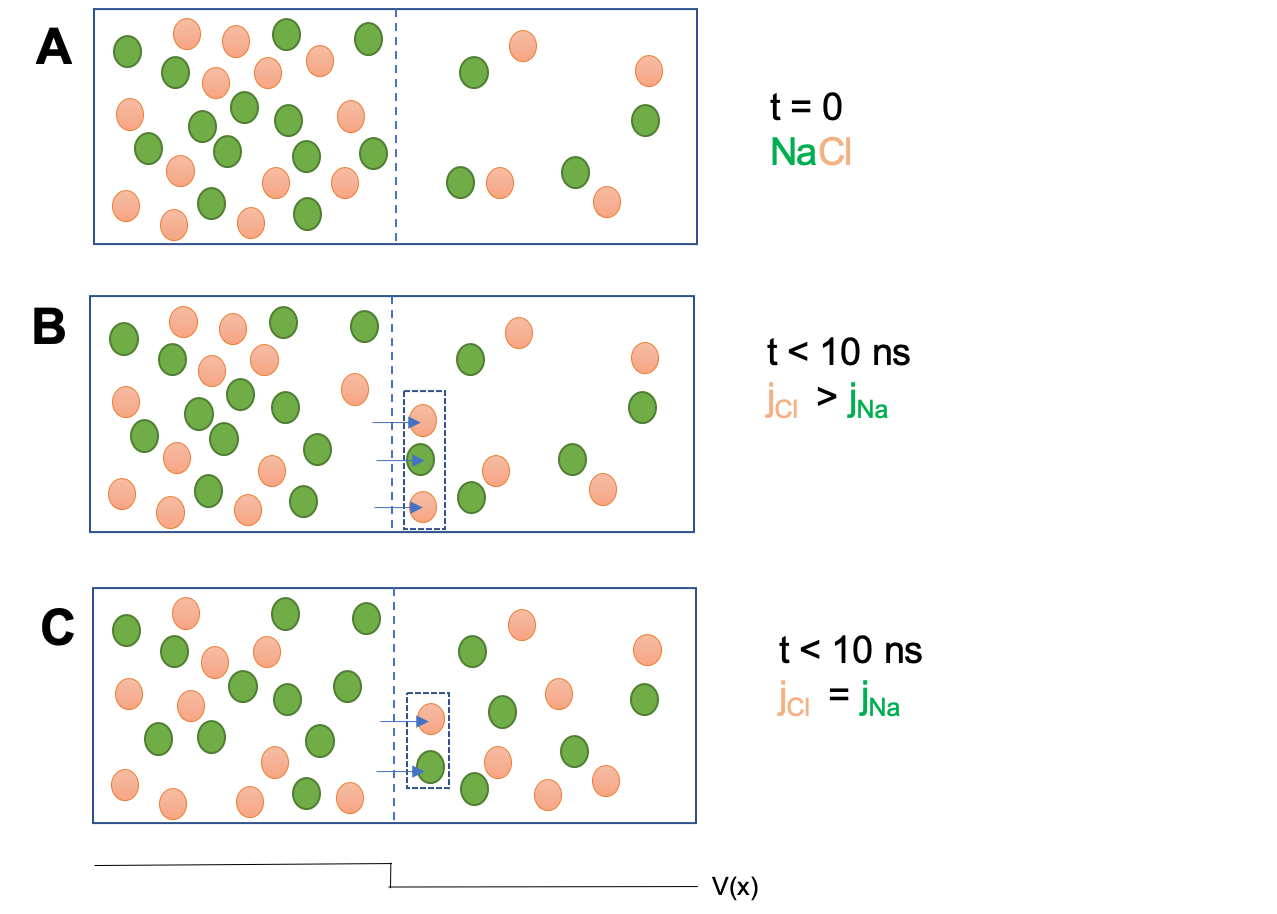
\includegraphics[width=0.8\textwidth]{Figures/Eldiff/Diffusionpot.png}
\end{center}
\caption{\textbf{Diffusion potential at the junction between two ionic solutions}. ({\bf A}) Initial condition with high concentration NaCl in the left compartment and low concentration NaCl in the right compartment. ({\bf B}) Since $D_{Cl} > D_{Na}$, we initially expect the flux of Cl$^-$ to be higher than the flux of Na$^+$. ({\bf C}) The net charge transfer in ({\bf B}) will give rise to a potential difference $\phi_d$ between the two compartments, which will prevent further charge accumulation. }
\label{Eldiff:fig:diffpot}
\end{figure}

We intuitively realize that both Na$^+$ and Cl$^-$ will diffuse towards the low-concentration compartment on the right-hand-side. Now, nature has it that not all ions diffuse equally fast, and the diffusive flux of a specific ion species will be proportional to its diffusion constant. From Table \ref{Sigma:tab:diffconsts}, we have that $D_{Na} = 1.33 \times 10^{-9}$ m$^2$/s, and $D_{Cl} = 2.03 \times 10^{-9}$ m$^2$/s in dilute solutions. Since $D_{Cl} > D_{Na}$, the rightward diffusive flux of Cl$^-$ will initially be larger than that for Na$^+$  (Fig. \ref{Eldiff:fig:diffpot}B). Diffusion thus acts as a charge separation process, resulting in an excess of positive charge in the left compartment and negative charge in the right compartment. The charge separation will in this way cause a potential difference ($\Delta \phi_d$) to arise between the compartments. Since $\Delta \phi_d$ stems from a diffusion process, it is often called the \textit{diffusion potential} \index{Diffusion potential}. Note that the diffusion potential arises due to differences in diffusion constants between different ions present. If all ions had identical diffusion constants, there would be no charge separation and thus no diffusion potential. 

The diffusion potential will oppose the on-going charge separation process by causing an electrical push on the anions (Cl$^-$) in the leftward direction, reducing the net rightward flux of Cl$^-$. Similarly, it causes a rightward pull on the cations (Na$^+$), increasing the net rightward flux of Na$^+$. Once it is gets big enough, $\Delta \phi_d$ will stabilize the system in a so-called quasi-steady state, where the net fluxes of Na$^+$ and Cl$^-$ have the same magnitude, and no further charge separation will take place (Fig. \ref{Eldiff:fig:diffpot}C). It has been shown that the extracellular medium of the brain only needs about 10 ns to reach this quasi-steady state \cite**{Solbra2018}. In the quasi-steady state, $\Delta \phi_d$ will still vary with time (hence the term "quasi"), and eventually become zero when the system is equilibrated and the ion concentrations are the same in the two compartments. However, whereas the quasi-steady state is reached within a few nanoseconds, the concentration-equilibration process occurs at an entirely different time scale and normally takes seconds to minutes. 

Since it happens so fast, computer simulations of the charge separation process must be run with a sub-nanosecond time resolution. To simulate it is therefore computationally demanding, and not even feasible for large systems. Fortunately, one can for many purposes obtain accurate predictions of both $\Delta \phi_d$ and ion concentration dynamics by using an electroneutral mathematical framework that does not model the charge relaxation process explicitly, but instead derives an analytical expression for the quasi-steady state potential, and assumes that the system is always in quasi-steady state. We shall introduce the modeling frameworks for electrodiffusive processes later on in this Chapter. 

In electrolyte theory, the diffusion potential is often called the \textit{liquid-junction potential} \index{Liquid-junction potential}, since it is most pronounced at the junction between two different ionic solutions \cite**{Aguilella1987,Sokalski2001}. Experimental neuroscientists should be acquainted with this term, since the determination of liquid-junction potentials is a common challenge when recording neural membrane potentials using patch clamp experiments. Through a process similar to that depicted in Fig. \ref{Eldiff:fig:diffpot}, only involving a larger number of different ion species, the liquid-junction potential develops at the junction between the pipette solution and the extracellular (or bath) solution, and give rise to a constant offset in the recordings, which must be estimated and corrected for \cite**{barry1991,neher1992}. The magnitude of the liquid-junction potential depends on the composition of the various ion solutions, but in patch-clamp experiments it is typically a few millivolts. Other familiar examples of diffusion potentials in neuroscience are the ion channel reversal potentials (eq. \ref{eq:Neuron:revpots}), which are essentially single-ion diffusion potentials, and the leakage reversal potential (eq. \ref{eq:Neuron:Eleak_GHK}), which is a diffusion potential depending on the differences in passive membrane permeabilities (replacing the role of diffusion constants) of the various ion species. 

Compared to the reversal potentials and liquid-junction potentials in patch clamp experiments, 
diffusion potentials in the bulk solutions or the intra- or extracellular space tend to be smaller in magnitude, and have not been that much studied in neuroscience. Below, we will outline the general physical theory for determining the electric potential in electrodiffusive processes.


\section{The Nernst-Planck equation}
\label{sec:Eldiff:NP}
\index{Electrodiffusion}
When modeling an electrodiffusive process, we keep track of the ion concentration dynamics of each individual ion species. The fundamental equation for doing that is the Nernst-Planck equation for the flux density (${\bf j_k}$ of an ion species $k$:
\begin{equation}
{\bf j_k} = - D_k {\bf \nabla} c_{k} - \frac{D_k z_k c_k}{\psi} {\bf \nabla} \phi, 
\label{eq:Eldiff:JNP}
\end{equation}
where ${D}_k$ is the diffusion constant (units $\mathrm{m^2/s}$), $z_{k}$ is the valency of ion species $k$, and $\psi=RT/F$ (units V) is defined by the gas constant ($R$), Faraday's constant ($F$) and the temperature ($T$). The first term on the right is Fick's law for diffusion, while the second term accounts for ions migrating in the electric field.  In eq. \ref{eq:Eldiff:JNP}, the the electrical mobility of the ions is $D_k/\psi$, and thus linearly related to their diffusion constant. This relationship is called the Einstein relation\index{Einstein relation}, and is valid for dilute solutions such as the extracellular or intracellular fluid \cite**{Grodzinsky2011}.

If we combine eq. \ref{eq:Eldiff:JNP} with the requirement of ion conservation:
\begin{equation}
\frac{\partial c_k}{\partial t} = -\nabla \cdot {\bf j_k},
\label{eq:Eldiff:general_ionconservation}
\end{equation}
we get the Nernst-Planck continuity equation:
\begin{equation}
\frac{\partial c_k}{\partial t} = {\bf \nabla} \cdot \left[{D_k} {\bf \nabla} c_k + \frac{D_k z_k c_k}{\psi}{\bf \nabla} \phi \right].
\label{eq:Eldiff:NP}
\end{equation}

Eq. \ref{eq:Eldiff:NP} gives us one equation for each individual ion concentration $c_k$, and to solve the system of equations, we are in need an additional equation for the additional variable $\phi$, the electrical potential which couples the dynamics of the individual ion species. There are two main approaches to this, the so-called \textit{Poisson-Nernst-Planck (PNP)} framework, or the so-called \textit{electroneutral} framework, both of which we will introduce below. 


\subsection{\blue{The Poisson-Nernst-Planck (PNP) framework}}
\label{sec:Eldiff:PNP}
\index{Poisson-Nernst-Planck equations}
The physically most detailed approach for defining $\phi$ in eq. \ref{eq:Eldiff:NP}) is to use Poisson's equation from electrostatics:
\begin{equation}
\nabla^2 \phi = -\rho/\epsilon
\label{eq:Eldiff:poisson}
\end{equation}
Here $\epsilon$ is the (local) permittivity of the medium, and the local charge density $\rho$ can be expressed as a function of the ionic concentrations:
\begin{equation}
\rho = F\sum_k z_k c_k + \rho_0.
\label{eq:Eldiff:PNPrho}
\end{equation}
When we model ion concentrations, we normally do not include absolutely all ion species that are present, but rather chose to keep track of the most important ones (such as Na$^+$, K$^+$, Cl$^-$ and Ca$^{2+}$). For technical reasons, we therefore added a static charge density $\rho_0$\index{Static charge density} to eq \ref{eq:Eldiff:PNPrho}, which to accounts for all charges not included in the set $c_k$. 

Combined with suitable boundary conditions, the PNP equations (eq. \ref{eq:Eldiff:NP} together with eq. \ref{eq:Eldiff:poisson}) can in principle be solved for arbitrary complex geometries using numerical methods, like the Finite Element Method (FEM). 


\subsection{\blue{The electroneutral framework}}
\label{sec:Eldiff:electroneutral}
\index{Electroneutral}
An alternative to the PNP approach is to replace the Poisson equation (eq. \ref{eq:Eldiff:poisson}) with the approximation that the bulk solution is electroneutral:
\begin{equation}
F \sum_k z_k c_k + \rho_0 = 0.
\label{eq:Eldiff:electroneutral}
\end{equation}
In practice, it is often more convenient to impose the electroneutrality approximation on differential form:
\begin{equation}
F \sum_k{z_k \frac{\partial c_k}{\partial t}} = 0.
\label{eq:Eldiff:electroneutral2}
\end{equation}

The electroneutrality approximation (eq. \ref{eq:Eldiff:electroneutral} or \ref{eq:Eldiff:electroneutral2}) can be imposed as a constraint when solving eq.\ref{eq:Eldiff:NP} by use of some numerical method. The constraint determines what $\phi$ must be at all points in space for there to be no charge accumulation anywhere in the extracellular or intracellular bulk solutions. As soon as reference point (i.e., ground, $\phi = 0$) is set, this problem has a unique solution.


\subsection{\blue{The difference between the PNP and electroneutral frameworks}}
\label{sec:Eldiff:CompareFrameworks}
To explain how the electroneutral framework differs from the PNP framework, we may use our previous cartoon example (Fig. \ref{Eldiff:fig:diffpot}) as a reference. As we there explained, the diffusion potential is (i) evoked by charge separation process that only lasts for $\sim 10$ ns, and is (ii) most pronounced at the junction between two solutions of different ionic composition. In neural tissue, nonzero charge densities are predominantly resolved in nano-meter thick layers around neuronal membranes \cite**{Grodzinsky2011,Gratiy2017}. 

The PNP framework explicitly models the nanosecond-fast charge relaxation processes (Fig. \ref{Eldiff:fig:diffpot}B), and must ensure that the ionic concentrations at all points sum up to the correct charge density (cf. eq. \ref{eq:Eldiff:PNPrho}). Since the deviance from electronutrality associated with $\rho$ involves a only very tiny fraction of the ions present \cite**{Aguilella1987}, stable PNP simulations require that $c_k$ is determined with an extreme precision. PNP simulations therefore require a spatiotemporal resolution smaller than nanometers and nanoseconds, and thus a very fine-grained description of the tissue where neuronal, glial and extracellular geometries are explicitly defined. This makes PNP simulations extremely computationally demanding, and not suited for estimating dynamics at the level of tissue. Applications in neuroscience have therefore been limited to studies of electrodiffusive processes taking place on a very tiny spatiotemporal scale, such as in dendritic spines or near and inside membranes \citeaffixed**{Leonetti2004,Lu2007,Lopreore2008,Nanninga2008,Gardner2011,Zheng2011,Pods2013,Gardner2015,lagache2019,cartailler2019}{see e.g.,}. See \citeasnoun**{Savtchenko2017} for a review of applications in neuroscience.

In contrast, the electroneutral framework circumvents the charge relaxation problem by assuming (and ensuring) that the system is always in quasi-steady (Fig. \ref{Eldiff:fig:diffpot}C), and uses the electroneutrality constraint (eq. \ref{eq:Eldiff:electroneutral} or \ref{eq:Eldiff:electroneutral2}) to derive the potential $\phi$ required for this to be the case. 
Although electroneutrality at a fundamental level is inconsistent with a non-zero $\phi$ (cf. eq. \ref{eq:Eldiff:poisson}), the electroneutral approach still give accurate predictions of both $c_k$ and $\phi$ under many circumstances \cite**{Feldberg2000}, since the fraction of ions associated with the deviance from electroeutrality is so small. In biophysical applications, it has been shown that the electroneutral approximation gives accurate results on spatiotemporal scales larger than micrometers and microseconds \cite**{Grodzinsky2011,Pods2017,Solbra2018}. The advantage with the electroneutral approach is that it, unlike PNP, gives stable solutions with an arbitrary coarse spatiotemporal resolution, making the electroneutral framework much more computationally efficient than the PNP framework . 

Both the PNP and electroneutral framework require numerical solutions based on finite element or finite difference methods. While the electroneutral framework is computationally much more efficient than the PNP framework, it is still too heavy to allow for simulations of large systems of neurons described with explicit geometries on today's computers. To our knowledge, the largest system that so far has been simulated in 3D on an electroneutral framework is small piece of tissue containing a bundle of 9 axons described with idealized geometries \cite**{ellingsrud2020}.


\subsection{\blue{Membrane boundary conditions}}
\label{sec:Eldiff:BCs}
To apply one of the electrodiffusive frameworks within a neuroscience context, one needs to represent the geometry and properties of the cellular membranes. In principle, we could compute all ionic concentrations and their coupling to the electrical potential by requesting that eq. \ref{eq:Eldiff:NP} should be fulfilled at all points in space, including both the extracellular space, the intracellular space and the membranes separating them. This could be achieved through having spatially and temporally varying diffusion coefficients $D_k$. However, the resolution with which one needed to represent $D_k$ would then be extremely high. Whereas $D_k$ could have a constant value in the intra- and extracellular bulk solutions, $D_k$ would over the membranes be (i) different in different spatial directions (i.e., normal to membrane surface versus parallel to membrane surface), (ii) vary with the very fine spatial resolution of an ion channel, and (iii) also be time dependent due to the opening/closing of ion channels. Unless the PNP scheme is applied to specifically model currents inside ion channels on a very small spatial scale (see e.g., \cite**{Gardner2011,Zheng2011}), such a fine-grained tensor description of $D_k$ does not seem like a reasonable approach. 

Instead, it is common to rather apply the PNP or electroneutral framework in two disjoint domains - the intra and extracellular - and to couple the dynamics in these two domains by introducing suitable boundary conditions at the membrane. In many applications, the membrane dynamics is then based on a Hodgkin-Huxley (HH) type formalism (c.f., Section \ref{sec:Neuron:membranecurrents}) also in PNP based (see e.g., \cite**{Lopreore2008,Pods2013,Gardner2015,Pods2017}) or electroneutral (see e.g., \cite**{Mori2006,Mori2009,Pods2017,ellingsrud2020}) models. When applying a HH formalism in this context, all transmembrane currents are made ion specific, i.e., they are described in terms of ionic fluxes over the membrane, so that for example a Na$^+$ current density ($i_{Na}$) in the standard HH formalism would need to be replaced with a Na$^+$ flux density, $j_{Na} = i_{Na}/(Fz_k)$. The leakage current ($i_L$ in eq. \ref{eq:Neuron:HHleak}) is in standard HH applications non-specific in terms of which ions that mediate it, but will in a PNP context have to be made ion specific by decomposing it into specific leakage fluxes of the various ions that are involved (see e.g., \cite**{Pods2013}). Apart from that, the HH formalism for membrane mechanisms can be applied in its original form also in an electrodiffusive context.

We note that in electroneutral frameworks, the electroneutrality constraint (eq. \ref{eq:Eldiff:electroneutral} or \ref{eq:Eldiff:electroneutral2}) applies only to the intra- and extracellular bulk solutions, and must be replaced with another constraint at the membrane, where a non-zero membrane (surface) charge density ($\eta^{mem}$ (C/m$^2$)) builds up the membrane potential according to the capacitor relationship:
\begin{equation}
c_m \phi_{m} = \pm \eta_{r}^{mem},
\label{eq:Eldiff:rhocap}
\end{equation}
or its temporal derivative: 
\begin{equation}
i_{cap} = \pm \frac{\partial \eta_{r}^{mem}}{\partial t},
\label{eq:Eldiff:rhocapt}
\end{equation}
Here, $c_m$ (F/m$^2$) in eq. \ref{eq:Eldiff:rhocap} is the specific membrane capacitance, and the left hand side of eq. \ref{eq:Eldiff:rhocapt} follows the definition is the capacitive membrane current density $i_{cap}$  (eq. \ref{eq:Neuron:HHcap}). In both equations, $r$ takes the indices $i$ (intracellular side of the membrane) or $e$ (extracellular side of the membrane), and the plus-sign should be used for $r=i$, and the minus-sign for $r=e$, a convention that follows from the definition $\phi_{m} = \phi_{i} - \phi_{e}$. The intra- and extracellular membrane charge densities in eq. \ref{eq:Eldiff:rhocap} or their derivatives in \ref{eq:Eldiff:rhocapt} are equal in magnitude and opposite in sign, since the charge stored on one side of a capacitor always balances the charge stored on the other side. 

For the electroneutrality constraint at the membrane (eq. \ref{eq:Eldiff:rhocap} or \ref{eq:Eldiff:rhocapt}) to be useful, $\eta_{r}^{mem}$ must be expressed in terms of the ion concentrations. That is, one needs an additional condition to specify the composition of ions that constitute $\eta_{r}^{mem}$ in eq. \ref{eq:Eldiff:rhocap} or mediate $i_{cap}$ in eq. \ref{eq:Eldiff:rhocapt}, so that ion conservation and a consistent charge-concentration relationship  at all points in space is ensured. Previous schemes for implementing the electroneutral framework vary somewhat in the approach taken to this:

\begin{itemize}
\item The electroneutral scheme with internal boundary conditions at membranes (ENM), derived the concentration profile of the membrane charge density $\eta_{r}^{mem}$ from a set of constraints as to how ion concentrations are distributed within the Debye-layer \cite**{Mori2006,Mori2009,Pods2017}.

\item The Kirchhoff-Nernst-Planck (KNP) scheme did not resolve Debye-layer concentrations, but let the membrane concentration profile follow from an assumption regarding how much various ion species contributed to the capacitive membrane current $i_{cap}$ \cite**{ellingsrud2020}.
\end{itemize}

Both electroneutral schemes (ENM and KNP) were designed so that the membrane concentration profiles were functions of, and similar to, the concentration profiles in the bulk solution close to the membrane. Although they differ in implementation details, the two schemes should be close to equivalent from a physics point of view, except at Debye layer-resolution close to the membrane.  In practice, only a very tiny fraction of the ions present are involved in building up the membrane potential, and the choice as to which ion species that actually constitute the membrane charge in eq. \ref{eq:Eldiff:rhocap} or \ref{eq:Eldiff:rhocapt} is probably quite unimportant for the overall system dynamics.


\section{\blue{Extracellular electrodiffusion in brain tissue}}
\label{sec:Eldiff:porous}
\index{sec:Eldiff:Tissue}
From here on, we will consider electrodiffusion at the scale of tissue, and we shall treat the tissue as a continuous porous medium. This is similar to how we treated the tissue as a continuous volume conductor in Chapter \ref{sec:VC}, the difference being that we now, in addition to keeping track of the extracellular potential ($\phi$), will be keeping track also of the extracellular concentrations ($c_k$) of all mobile ion species within the medium. 

In standard applications of VC theory, the neurodynamics is computed with multicompartment (MC) models in an independent step (Step 1) under the assumption that it is independent of whatever goes on in the extracellular space. The transmembrane neuronal currents are then, in a next step (Step 2), considered as distributed current sources and sinks within the tissue. A similar approach can been taken to study extracellular electrodiffusion, e.g., by combining MC neuron models (Step 1) with an electroneutral electrodiffusive framework (Step 2) such as the so-called Kirchhoff-Nernst-Planck (KNP) framework presented in \cite**{Solbra2018}. The procedure is then:

\begin{itemize}
\item {\bf Step 1:} Compute neurodynamics using a standard MC framework (Chapter \ref{sec:Neuron}). Unlike in the standard MC+VC scheme, where the different kinds of transmembrane currents, such as leakage currents, capacitive currents, and ion specific active currents, can be grouped into a single source variable $C$ for the total current source density (CSD) at each segment, an electrodiffusive treatment requires that all neural sources are expressed as a set of ion specific sources, i.e., one source $f_k$ per ion species $k$ and an additional capacitive neuronal membrane current source density, $C_e^{cap}$ (proportional to $i_{cap}$ in eq. \ref{eq:Eldiff:rhocapt}), the only source term not accounted for in the set $f_k$. These variables, along with other relevant variables, will be defined properly below (Section \ref{sec:Eldiff:porous}).

\item {\bf Step 2:} Use an electrodiffusive framework to compute the dynamics of $c_k$ and $\phi$ in the extracellular space when "receiving" input from discrete neuronal sources computed in Step 1 (Fig. \ref{Eldiff:fig:KNPmesh}). The Nernst-Planck continuity equation (eq. \ref{eq:Eldiff:NP}) is then applied exclusively to the extracellular space, and the neural output is expressed through the source terms ($f_k$ and  $C_e^{cap}$). In the following, we will present the KNP framework for extracellular electrodiffusion within this two-step scheme.
\end{itemize}

\begin{figure}[!ht]
\begin{center}
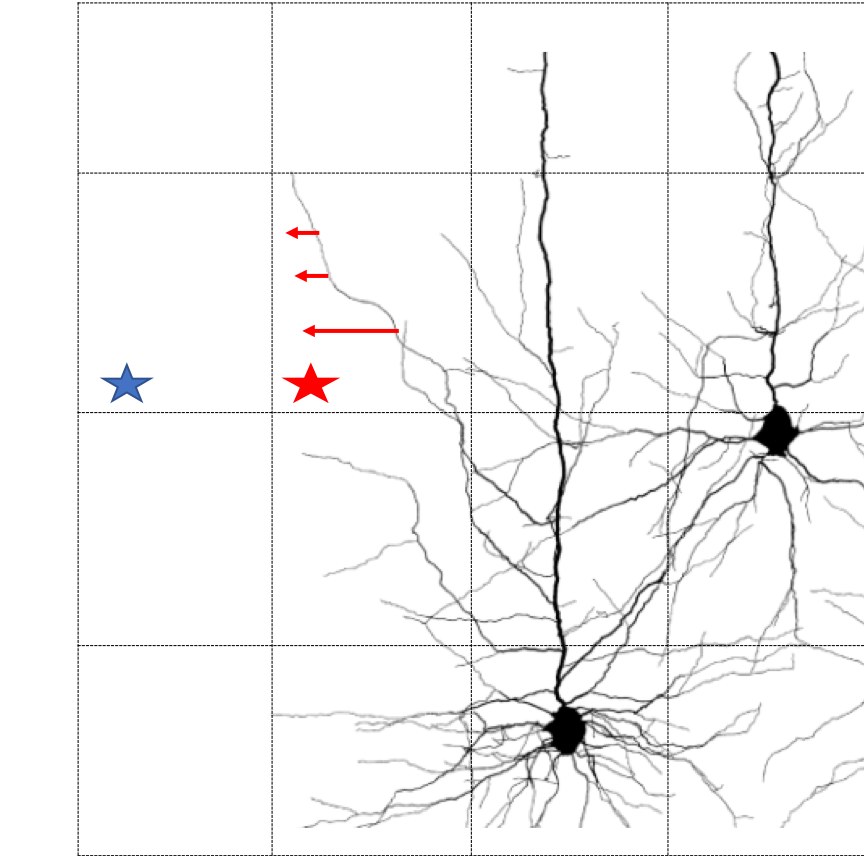
\includegraphics[width=0.5\textwidth]{Figures/Eldiff/KNP.png}
\end{center}
\caption{\textbf{KNP scheme}. Blue star: Mesh cell containing no neuronal sources, so that $C=0$. Red star: Mesh cell containing neural sources. Here $C$ can be computed by summing over all neuronal transmembrane currents, including the capacitive current, and dividing by the volume of the mesh cell. \ghnote{LAGE LITT MER INFORMATIV FIG HER OM VI SKAL HA FIG HER.}}
\label{Eldiff:fig:KNPmesh}
\end{figure}


\subsection{\blue{Continuous, porous medium approximation for electrodiffusion in tissue}}
\label{sec:Eldiff:porous}
\index{Continuous medium}
\index{Porous medium}
In Section \ref{sec:Sigma:continuous}, we introduced the continuous, porous medium approximation for coarse grained volume conduction in brain tissue, and we will use a similar approximation for electrodiffusive processes through the tissue. As in Section \ref{sec:Sigma:continuous}, 
the key parameters for defining the porous medium are the extracellular volume fraction $\alpha$ and the tortuosity, $\lambda$ (Fig. \ref{Eldiff:fig:porous}). However, unlike what we did in Section \ref{sec:Sigma:continuous}, where our reference volume was the tissue as a whole, we shall here follow the convention that we use as reference volume only the fraction $\alpha$ of tissue that is extracellular space \cite**{Sykova2008}. As we shall see, this convention offers the most natural definition of the extracellular concentrations. 

\begin{figure}[!ht]
\begin{center}
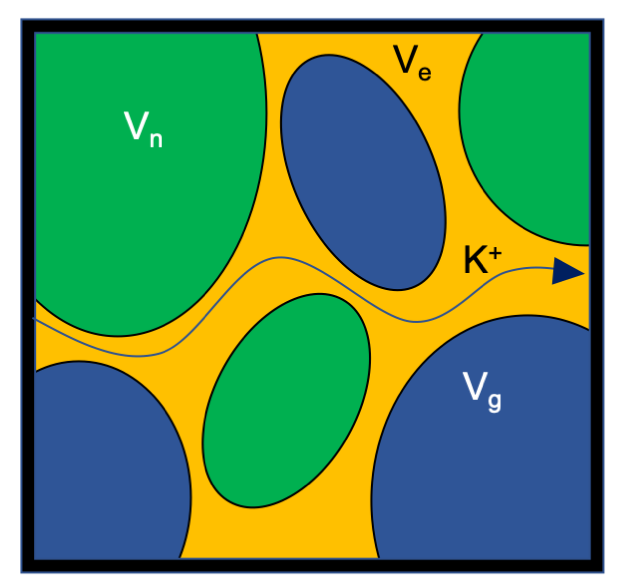
\includegraphics[width=0.5\textwidth]{Figures/Eldiff/Porous.png}
\end{center}
\caption{\textbf{Tortuous, porous medium.}  Sketch of a cross-section of a piece of neural tissue. Extracellular space (yellow) occupies a fraction $\alpha$ (about 0.2 of the total tissue volume), while neurons and glial cells occupy about equally much of the remaining space. The extracellular space has a highly tortuous structure. We consider tissue transport processes that are confined to occur only in the extracellular part of the tissue. Detours around neuronal and glial obstacles are accounted for by the tortuosity $\lambda$. 
\tvnnote{kanskje med panel B en zoomet ut versjon der det ser mer homogent ut? Hadde Klas allerede laget en lignende figur til Sterratt? }
}
\label{Eldiff:fig:porous}
\end{figure}

If we define all extracellular variables relative to the extracellular volume fraction  (Fig. \ref{Eldiff:fig:porous}), they can be defined as:

\begin{itemize}
\item $c_k$ (units $\mathrm{mol/m^3}$ = mM) is the extracellular concentration of an ion species $k$, defined as the number of extracellular ions of species $k$ (in mol) per extracellular volume unit (which is a fraction $\alpha$ of the tissue volume unit). The motivation for using the extracellular volume fraction as the reference volume is that concentrations defined in this way will be the "real" extracellular concentration, i.e., the concentration experienced by a neural membrane, 

\item $\rho_e$ (units $\mathrm{C/m^3}$) is the extracellular charge density
of an ion species $k$, defined as the number of extracellular ions of species $k$ (in mol) per extracellular volume unit (which is a fraction $\alpha$ of the tissue volume unit).

\item ${\bf j_k}$ (units $mol/\mathrm{m^2s}$) is the extracellular flux density of an ion species $k$, defined as the number of extracellular ions (in mols) crossing an extracellular unit cross- section area (which is a fraction $\alpha$ of a unit tissue cross-section area) per second.

\item  ${\bf i_e}$ (units $\mathrm{A/m^2}$) is the extracellular current density, defined as extracellular current per per extracellular unit cross-section area. In comparison, the current density ${\bf i}$ in Chapter \ref{sec:VC} was defined as extracellular current per unit tissue cross-section area, which means that ${\bf i_e} = {\bf i}/\alpha$.

\item $\tilde{D}_k$ (units $\mathrm{m^2/s}$) is the effective diffusion constant \index{Diffusion constant} for ion species $k$ in the extracellular medium. It is defined so that the diffusive flux is given by ${\bf j_k^{diff}} = -\tilde{D}_k \nabla c_k$ \cite**{nicholson2001}. The effective diffusion constant accounts for the fact that diffusing ions face obstacles (neurites) along their path forcing them take detours, reflected through a tortuosity $\lambda$ which has a value of about 
$1.6$ in the extracellular space \cite**{Nicholson1998}. The effective diffusion constant is given by:
\begin{equation}
\tilde{D_k} = \frac{D_k}{\lambda^2}, 
\label{eq:Eldiff:diffconst}
\end{equation}
where $D_k$ is the diffusion constant for an ion species $k$ in the pure (unhindered) extracellular solution. The fact that diffusing ions are confined the stay only in the extracellular volume fraction $\alpha$ is already accounted for in the flux definition. 

\item $\sigma_e$ (units S/m) is the tissue averaged extracellular conductivity for extracellular current densities defined as ${\bf i_e}$. As we show later, $\sigma_e$ can be expressed as a function of ion concentrations:
\begin{equation}
\sigma_e = \frac{F}{\psi}\sum_{k} \tilde{D}_k z_{k}^2 c_{k}.
\label{eq:Eldiff:sigma1}
\end{equation}
Here $z_{k}$ is the valency of ion species $k$, and $\psi=RT/F$ is defined by the gas constant ($R$), Faraday's constant ($F$) and the temperature ($T$). Since $\sigma_e$ relates to ${\bf i_e}$ in the same way that the tissue conductivity, $\sigma_t$, related to ${\bf i_t}$ in Chapter \ref{sec:VC}, $\sigma_e = \sigma /\alpha$.

\item $f_k$ (units mol/m$^3$) is the ion-flux-source density, i.e., the local neuronal output of an ion species $k$ per per extracellular volume unit. It is essentially is the ion-dynamics counterpart to the current-source-density (CSD) presented earlier (eq. \ref{eq:VC:CSD1}).

\item $C_e$ (units A/m$^3$) is the current source density, i.e., the local neuronal output current per extracellular volume unit. $C_e = C/\alpha$ where $C$ (as defined in Chapter \ref{sec:VC}) is neuronal output current per tissue volume unit.
\end{itemize}


\subsection{\blue{Dynamics of ion concentrations}}
\label{sec:Eldiff:ionconcentrationdynamics}
In the coarse-grained description, using the effective diffusion constant, $\tilde{D}_k$, the flux density (${\bf j_k}$) of an ion species $k$ is given by:
\begin{equation}
{\bf j_k} = - \tilde{D}_k {\bf \nabla} c_{k} - \frac{\tilde{D}_k z_k c_k}{\psi} {\bf \nabla} \phi.
\label{eq:Eldiff:JNP}
\end{equation}
The first term on the right hand side of eq. \ref{eq:Eldiff:JNP} is the ionic flux density due to diffusion (${\bf j_{k}^\text{diff}}$), and the second term is the additional flux density due to electrical drift along gradients in the extracellular potential $\phi$ (${\bf j_{k}^\text{drift}}$). 

The general continuity equation for an ion species $k$ is,
\begin{equation}
\frac{\partial c_k}{\partial t} = - \nabla \cdot {\bf j_k} + f_k,
\label{eq:Eldiff:salamander}
\end{equation}
where we have included the neuronal source term $f_k$. If we insert the electroduffusive flux density (eq. \ref{eq:Eldiff:JNP}) into eq. \ref{eq:Eldiff:salamander}, we get the Nernst-Planck continuity equation:
\begin{equation}
\frac{\partial c_k}{\partial t} = {\bf \nabla} \cdot \left[ \tilde{D}_k {\bf \nabla} c_k + \frac{\tilde{D}_k z_k c_k}{\psi} {\bf \nabla} \phi \right] + f_k.
\label{eq:Eldiff:NP}
\end{equation}
This equation is the fundamental equation in the KNP scheme. Eq. \ref{eq:Eldiff:NP} gives us one equation for each individual ion concentration $c_k$, and to solve the system of equations, we are in need an additional equation for the additional variable $\phi$. 


\subsection{\blue{Dynamics of the extracellular potential}}
\label{sec:Eldiff:electrodynamics}
From the equations for ion concentration dynamics (eqns. \ref{eq:Eldiff:JNP}-\ref{eq:Eldiff:NP} ) we can derive a corresponding set of equations for net charge dynamics. This will also allow us to derive the expression for $\phi$ that we need in order to solve the Nernst-Planck equation (eq. \ref{eq:Eldiff:NP}).  It will also show us how they relate to to the VC theory presented in Chapter \ref{sec:VC}.

If we multiply eq. \ref{eq:Eldiff:JNP} by $F\cdot z_k$ and sum over all ion species $k$, we get the extracellular current density:
\begin{equation}
{\bf i_e} = F\sum_k {z_k {\bf j_k}} = -\sum_k{F z_k \tilde{D_k}{\bf \nabla} c_{k}} - F\sum_{k} \frac{\tilde{D_k} z_{k}^2}{\psi}c_{k} {\bf \nabla}{\phi}, 
\label{eq:Eldiff:INPa}
\end{equation}
where the first term on the right hand side is the diffusive current density ${\bf i_e^\text{diff}}$, and the second term is the Ohmic drift current density ${\bf i_e^\text{drift}}$. Since we know from earlier that the drift current density should equal $- \sigma_e \nabla \phi$  (cf. eq. \ref{eq:VC:ohmici}) we may identify the the conductivity $\sigma_e$ of the extracellular medium as \cite**{Koch1999}:
\begin{equation}
\sigma_e = \frac{F}{\psi}\sum_{k} \tilde{D}_k z_{k}^2 c_{k},
\label{eq:Eldiff:sigma}
\end{equation}
as we postulated in eq. \ref{eq:Eldiff:sigma1}. With this, we can write eq. \ref{eq:Eldiff:INPa} on the simpler form:
\begin{equation}
{\bf i_e} = - \sum_k{F z_k \tilde{D_k}{\bf \nabla} c_{k}} - \sigma_e{\bf \nabla}{\phi},
\label{eq:Eldiff:INP}
\end{equation}

Likewise, if we multiply eq. \ref{eq:Eldiff:salamander} by $F\cdot z_k$ and sum over all ion species, we get the continuity equation for charge: 
\begin{equation}
\frac{\partial \rho_e}{\partial t} =  \nabla \cdot \left (\sum_k{F z_k \tilde{D_k}{\bf \nabla} c_{k}} + \sigma_e\nabla\phi  \right)  + C_e^{ion}.
\label{eq:Eldiff:chargecontinuity}
\end{equation}
We have here introduced the extracellular charge density (define as extracellular charge per tissue unit volume), 
\begin{equation}
\rho_e = F \sum_k z_k c_k + \rho_{0e},  
\label{eq:Eldiff:roen}
\end{equation}
and the ionic current source, 
\begin{equation}
C_e^{ion} = F \sum_k z_k f_k. 
\label{eq:Eldiff:csden}
\end{equation}
The term $\rho_{0e}$ in eq. \ref{eq:Eldiff:roen} represents a static extracellular charge density representing charged macromolecules and any species' of ions that are not included in the set $c_k$, and which is assumed to be constant in time and space. The index "ion" in eq. \ref{eq:Eldiff:csden} signifies that this source term exclusively accounts for the sources $f_k$ mediated by ions that pass through the neuronal membrane and enters or leaves the extracellular space in eq. \ref{eq:Eldiff:NP}. Importantly, $C_e^{ion}$ is not identical to the total CSD, which contains an additional capacitive component that accounts for the accumulation of a charge density $\rho_e^{mem}$ (defined as membrane charge per extracellular unit volume) at the exterior side of the neuronal membrane:
\begin{equation}
C_e = C_e^{ion} + C_e^{cap} = F \sum_k z_k f_k - \frac{\partial \rho_{e}^{mem}}{\partial t}.
\label{eq:Eldiff:CSDdecomposed}
\end{equation}
$C_e^{cap}$ interprets as the neuronal capacitive membrane current per extracellular unit volume (see Fig. \ref{Eldiff:fig:Ccap}), and the negative sign in front of the last term in \ref{eq:Eldiff:CSDdecomposed} follows from the fact that an outwards capacitive current (i.e., a source) implies an accumulation negative charge on the exterior side of the membrane. 

\begin{figure}[!ht]
\begin{center}
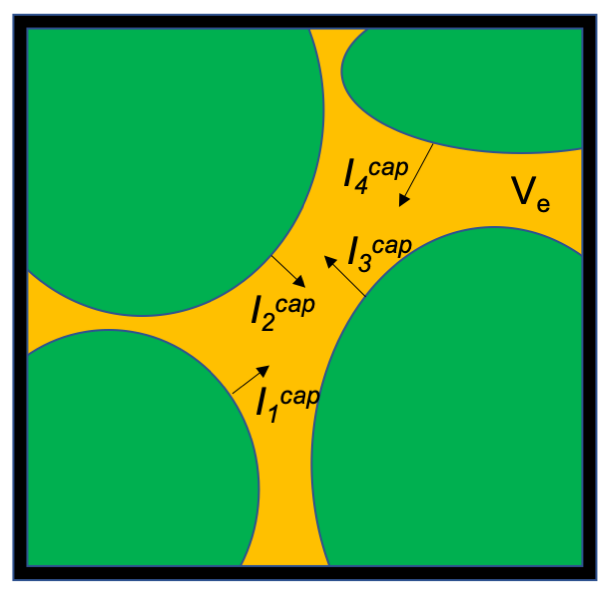
\includegraphics[width=0.5\textwidth]{Figures/Eldiff/KNP_Cap_illustration.png}
\end{center}
\caption{\textbf{Capacitive current sources}. Illustrated in terms of a finite volume of tissue, the capacitive current source density is the sum of capacitive currents entering the extracellular space from cells (green), divided by the fraction of the tissue volume that is extracellular (orange), i.e., $C_e^{cap} = \sum_k I_k^{cap}/V_e$. It can be interpreted as the accumulation of an extracellular charge density, which, since the bulk solution is assumed to be electroneutral, is associated exclusively by the charge accumulating at the exterior neural membranes.}
\label{Eldiff:fig:Ccap}
\end{figure}

Let us now look at the charge density, $\rho_e$ at the left hand side of eq. \ref{eq:Eldiff:chargecontinuity}. In general, $\rho_e$ could be composed of free charges in the extracellular bulk solution as well as charges bound to the outside of the neural membrane, i.e., we could have $\rho_e = \rho_e^{free} + \rho_e^{mem}$. However, as we have argued earlier, the bulk solution is very close to electroneutral, and if we assume perfect bulk electroneutrality ($\rho_e^{free} = 0$), we must have that $\rho_e=\rho_e^{mem}$. We can then combine eq. \ref{eq:Eldiff:chargecontinuity} with eq. \ref{eq:Eldiff:CSDdecomposed} to arrive at:

\begin{equation}
\nabla \cdot (\sigma_e\nabla\phi) = - C_e - F \nabla \cdot \left (\sum_k{z_k \tilde{D_k}{\bf \nabla} c_{k}} \right).
\label{eq:Eldiff:eldiffCSD2}
\end{equation}

Provided that the neuronal current sources $C_e$ and the extracellular ion concentrations $c_k$ are known at a given time, eq. \ref{eq:Eldiff:eldiffCSD2} can be solved for $\phi$. This solution for $\phi$ can be then be inserted into the Nernst-Planck system of equations (eq. \ref{eq:Eldiff:NP}), 
which can be solved for the temporal development of $c_k$ using some suitable numerical framework. It is the combination of eqns. \ref{eq:Eldiff:NP}) and \ref{eq:Eldiff:eldiffCSD2}, with $C_e$ as given in eq. \ref{eq:Eldiff:CSDdecomposed}, that defines the KNP scheme. 


\subsection{\blue{Comparison with volume conductor theory}}
Eq. \ref{eq:Eldiff:eldiffCSD2} is the electrodiffusive counterpart to eq. \ref{eq:VC:CSD2}, that we used as starting point in standard VC theory. For a more direct comparison, we can multiply eq.  \ref{eq:Eldiff:eldiffCSD2} with the extracellular volume fraction $\alpha$, and get:
\begin{equation}
\nabla \cdot (\sigma\nabla\phi) = - C - F\alpha \nabla \cdot \left (\sum_k{z_k \tilde{D_k}{\bf \nabla} c_{k}} \right).
\label{eq:Eldiff:eldiffCSD22}
\end{equation}
Comparing eq. \ref{eq:Eldiff:eldiffCSD22} and eq.  \ref{eq:Eldiff:eldiffCSD2}, we see that the difference is the last term in eq. \ref{eq:Eldiff:eldiffCSD22}, which is the diffusive contribution not accounted for in \ref{eq:VC:CSD2}. As eq. \ref{eq:Eldiff:eldiffCSD2} shows, also diffusive processes can contribute to the genesis of extracellular potentials, and if present, they could give rise to a non-zero $\phi$ even in the absence of neuronal sources ($C = 0$). Diffusive currents can thus be seen as an additional "source" for generating extracellular potentials \cite**{Halnes2017}. 

As we showed in Chapter \ref{sec:VC}), eq. \ref{eq:VC:CSD2} (which is eq.  \ref{eq:Eldiff:eldiffCSD22} without the last term) allows us to derive an analytical expression for the electrical potential at all points in space once the $C$ is known. In comparison, the electrodiffusive counterpart (eq. \ref{eq:Eldiff:eldiffCSD22}) is more demanding to work with, as it requires finite element or finite difference solutions of the ion concentration dynamics in the three-dimensional extracellular space \cite**{Solbra2018}. 


\subsection{\blue{Bi- and tri-domain models}}
\label{sec:Eldiff:domain}
\index{Domain models}
We should note that there exist a different category of tissue-scale electroneutral models, which have been inspired from by the bi-domain model by Eisenberg \cite**{eisenberg1970}, which has previously been used to simulate cardiac tissue \cite**{henriquez1993,sundnes2006,Mori2008}. 

In this category, the most advanced models for brain tissue are the tri-domain models, where three the domains represent (i) neurons, (ii) extracellular space, and (iii) a glial syncytium, i.e., a populations of gap-junction coupled glial cells \cite**{OConnell2016,tuttle2019}. Simpler, related models include the bi-domain model for neurons and extracellular space \cite**{Mori2015}, or 1D models of glial K$^+$ buffering, where only the glial and extracellular domain were included \cite**{Gardner-Medwin1983,Chen2000,Halnes2013}.

The domain models do not model individual cells, but represents tissue as a (volume-averaged) continuum. All domains "exist" in parallel at each point in space, and are defined through a set of domain-specific variables (e.g., domain-voltage, domain-ion concentrations, domain-osmolarity, domain-volume fractions etc.). The domains interact locally through a set of (Hodgkin-Huxley type) membrane mechanisms, while spatial electrodiffusive transports may occur \textit{within} the domains. 

In the tri-domain models \cite**{OConnell2016,tuttle2019}, intra-domain ion transport was assumed to occur in the glial and extracellular domain, but not the neural domain. The rationale behind that assumption was that a type of glial cells called astrocytes tend to be gap-junction coupled into a syncytium. In the syncytium, the intracellular space is more or less continuous in the same way that the extracellular space is continuous. Transport processes within the syncytium is then equivalent to extracellular transport in the sense that both take place in a continuous, tortous space. In contrast, neurons do not form synciti, and are "local" in the sense that no intracellular transport over distances occur within the neural domain (Fig.\ref{Eldiff:fig:domainmodel}). 

\begin{figure}[!ht]
\begin{center}
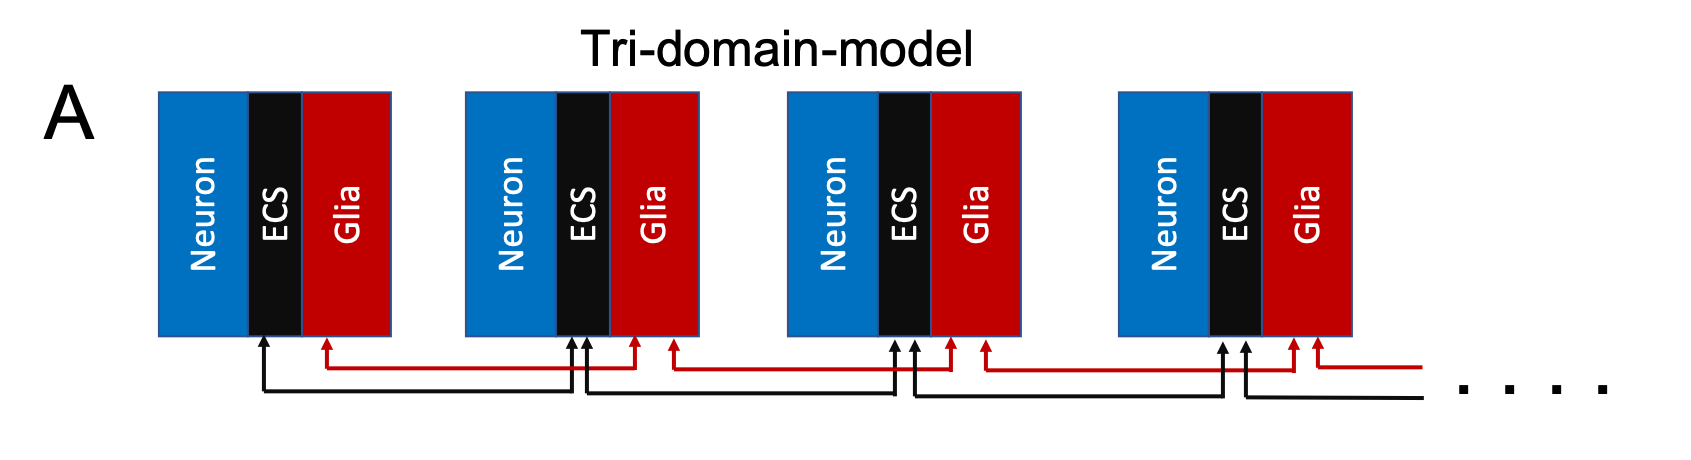
\includegraphics[width=0.8\textwidth]{Figures/Eldiff/Tridomain.png}
\end{center}
\caption{\textbf{Tri-domain model of brain tissue.} The domains represent neurons, extracellular space (ECS) and glial cells. The domains interact locally through transmembrane currents. Spatial ellectrodiffusion (arrows) occur within the ECS and glia domains, but not in within neuronal domain.The spatial dynamics can, in principle, occur in all directions (3D),but a 1D illustration was used in the figure. 
}
\label{Eldiff:fig:domainmodel}
\end{figure}

Domain models are suited to model brain dynamics taking place on large spatiotemporal scale, such as the wave of K$^+$ and the slow, DC-like diffusion potentials and glial buffering potentials that take place during the pathology of spreading depression \cite**{Mori2015,OConnell2016,tuttle2019}. However, as these models treat all aspects of brain tissue as a homogeneous, coarse-grained continuum, they are not suited to model the faster fluctuations of extracellular potentials which are recorded in MUA, LFP and EEG, as these depend strongly on morphologies of neurons \cite**{Einevoll2013}. 


\section{\blue{Do diffusion potentials matter?}}
\label{sec:Eldiff:estimates}
\index{Diffusion potential}
Due to the computational challenges they impose, it is tempting to make the assumption that diffusive currents contribute so little to the extracellular potential that we don't have to bother with them. This is what normally is being done, as most theoretical studies of extracellular potentials are based on standard VC theory. For most purposes, this is probably a good approximation, but its validity depends on one of the two following criteria being met:

\begin{enumerate}
\item C1: The magnitude of diffusive currents is much smaller than the magnitude of Ohmic drift currents.
\item C2: The frequency of diffusive currents is much lower than the frequency of the CSD and the Ohmic drift currents. 
\end{enumerate}

The first criterion is general and quite intuitive. If C1 holds, the last term in eq. \ref{eq:Eldiff:eldiffCSD2} becomes much smaller than the other two terms, and standard VC theory will give accurate predictions of $\phi$. As we shall see below, it is quite likely that C1 is violated under many physiological conditions. If so, the second criterion (C2) may still come to our rescue. In most experiments, extracellular potentials are recorded using electrode systems with a lower cut-off frequency of 0.1-1 Hz \cite**{Einevoll2007}. As diffusive currents are proportional to concentration gradients, which generally vary at a much slower time scale than $\phi$, diffusive contributions to $\phi$ are often direct-current (DC) like, i.e., they vary very slowly with time, and if they vary slowly enough, they will not be picked up in recordings using standard electrode systems, but only in experiments using DC electrodes. The question regarding their contribution to standard measurements is then whether they vary slowly enough. 

In the two following subsections we shall explore when and to which degree the criteria C1-C2 are likely to be met under physiological conditions.

\subsection{\blue{Magnitude of diffusion potentials.}}
To make some crude estimation of the magnitude that we can expect diffusion potentials to have in neural tissue, we make the following simplifications of eq. \ref{eq:Eldiff:eldiffCSD2}): Firstly, diffusion potentials depend solely on extracellular concentration gradients, and not on the instantaneous activity of neurons. Let us therefore assume that $CSD = 0$, and consider the extracellular dynamics is governed by:
\begin{equation}
\nabla \cdot (\sigma_e\nabla\phi_d) = - \nabla \cdot \left (\sum_k{F z_k \tilde{D_k}{\bf \nabla} c_{k}} \right), 
\label{eq:Eldiff:eldiffCSD3}
\end{equation}
where we have denoted the potential $\phi_d$ since, in this case, it will exclusively be evoked by diffusion. Let us further consider a system with closed boundaries, so that no current can enter or leave the system. In that case, we may simply skip the first nabla, and take:
\begin{equation}
\sigma_e\nabla\phi_d = -\sum_k{F z_k \tilde{D_k}{\bf \nabla} c_{k}}, 
\label{eq:Eldiff:diffpot}
\end{equation}
Essentially, eq. \ref{eq:Eldiff:diffpot} states that the Ohmic drift current and diffusive current must cancel each others at each point in space, i.e., that if no current enters the system from the outside, no net current should be observed anywhere inside the system. The diffusion potential is thus the potential that we must have in the system for this to be the case. 

Finally, due to the linearity in eq. \ref{eq:Eldiff:diffpot}, the diffusion potential between two points in space is a direct function of the the ionic concentrations at these two points. Hence, it is sufficient for our task to consider a simple two-compartment system (like that in Fig. \ref{Eldiff:fig:diffpot}). For two-compartment systems, eq. \ref{eq:Eldiff:diffpot} further simplifies to:

\begin{equation}
\Delta \phi_d = \frac{F}{\bar{\sigma_e}} \sum_k{z_k \tilde{D}_k \Delta c_k}
\label{eq:Eldiff:diffpot2}
\end{equation}
where $\Delta c_k = c_{k}^{2} - c_{k}^{1}$ and $\Delta \phi_d = \phi_d^{2} - \phi_d^{1}$ denote the concentration and potential difference between compartments 1 and 2. Within each compartment, $\sigma_e$ can be determined from the ionic concentrations by use of eq. \ref{eq:Eldiff:sigma1}. However, since we for this problem need the conductivity experienced by an Ohmic current traveling between the two compartments, we have in eq. \ref{eq:Eldiff:diffpot2} used the average $\sigma_e$ of the two compartments:
\begin{equation}
\sigma_e = \frac{F}{2\psi}\sum_{k} \left(\tilde{D}_k z_{k}^2 c_{k}^{1} + \tilde{D}_k z_{k}^2 c_{k}^{2} \right).
\label{eq:Eldiff:sigma2}
\end{equation}

Based on eq. \ref{eq:Eldiff:diffpot2}, we make some estimates of the magnitude of the diffusion potential for some test examples.

\begin{itemize}

\item {\bf Diffusion potential under spreading depression:} The most extreme extracellular concentration shifts in the brain occur under the pathological condition called spreading depression, where the extracellular K$^+$ concentration can change by several tens of millomolars. In an an example from hippocampus, the K$^+$ concentration was about 30 mM higher at the bottom hippocampal layer than at the top hippocampal layer (Fig. 1a in \cite**{Herreras1993}). In that experiment, only K$^+$ concentrations were recorded. However, we may give a crude estimate of the diffusion potential between the top and bottom of hippocampus by making some simple assumptions of the other ion concentrations: (i) We assume that the top layer of hippocampus remained at baseline concentrations. In the experiment, this seemed to be close to the case for $c_K$ \cite**{Herreras1993}. In the top layer, we may therefore assume some rather typical baseline concentrations with $c_{Na} = 150$ mM, $c_{K} = 3$ mM and $c_{Cl} = 153$ mM. (ii) In the bottom layer, we assume that the $c_K$ was 30 mM above baseline, and that the increase in $c_K$ was compensated by an identical decrease in $c_{Na}$, so that electroneutrality was preserved. A plausible mechanism behind this would be that all concentration shifts were due to neuronal AP firing, i.e., neurons exchanging Na$^+$ for K$^+$. With these assumptions, we have $c_{Na} = 120$ mM, $c_{K} = 33$ mM and $c_{Cl} = 153$ mM in the bottom layer. Plugging the top layer and bottom layer concentrations into eq. \ref{eq:Eldiff:diffpot2}, we obtain a diffusion potential $\Delta \phi_d \sim 1$ mV across the hippocampal depth.

\item {\bf Diffusion potential in cortex during neuronal hyperactivity:} In several experimental papers, extracellular concentration shifts of selected ions have been recorded during induced neuronal hyperactivity and seizure activity \cite**{kriv1975,nicholson1978,Dietzel1982,somjen1986,Dietzel1989}. The main focus of these works are typically on $c_K$, which is the most critical extracellular concentration due to its low baseline value. In these experiments, $c_K$ can typically change from a baseline value around 3 mM up to a ceiling level between 8-12 mM before the dynamics becomes pathological and is driven into spreading depression. Dietzel et al. estimated the concentration shifts in both $c_{K}$, $c_{Na}$ and $c_{Cl}$, and cased on a series of recordings, they estimated that the maximal diffusion potential that could be expected under their experimental condition was 0.4 mV \cite**{Dietzel1989}.

\item{\bf Diffusion potential during normal activity:} It is difficult to find experimental data that allows us to estimate diffusion potentials in the brain under "normal" conditions, and the question as to whether concentration gradients are present in a given brain region probably depends on the processing state it is in. However, recordings from anesthetized cat cortex have shown that even during the resting state, $c_K$ may exhibit small-amplitude (0.5 mM) fluctuations \cite**{MCCREERY1983}. In experiments recording the response in cortex to moderate (not seizure inducing) stimuli applied in the thalamus, cortical $c_K$ increases were found to have a depth profile, and vary by about 2 mM between different cortical layers \cite**{Cordingley1978}. Thus, it seems likely that there should be some concentration gradients present in neural systems, and that e.g., a concentration difference of about 1 mM between the top and bottom of cortex or hippocampus would not be unlikely under normal processing. If we repeat the calculation from spreading depression, but assume that $c_{K}$ and $c_{Na}$ in the bottom layer were increased/decreased by 1 mM instead of 30 mM, we get a diffusion potential of about $33 \mu$V. This is of the same magnitude as potentials typically recorded in LFP recordings. 

\end{itemize}

Based on the crude estimates above, it is likely that many experimental conditions can contain diffusion potentials of the same magnitude as the potentials recorded in extracellular recordings, such as the LFP. 


\subsection{\red{GH: Frequency of diffusion potentials}}
\ghnote{Krevende kapittel. Sammenligne noen powerspectra her. Regne ut et par selv, ala Gratiy. Ser for meg at vi kanskje kjoerer eksemplene fra forrige delkap, og da lar konsentrasjonene falle til utjevining vha. diffusjon, samt et tilleggseksempel der vi lar dem falle eksponensielt med ulike tidskonstanter og bestemmer hvor raskt det maa gaa for at det skal fanges opp f.eks. ved 0.1 Hz. Da trenger vi paalitelige powerspectra fra eksperimentelle maalinger som vi kan sammenligne med. } 

Previous computational studies have predicted that effects of diffusion on extracellular potentials are not necessarily small, but tend to be very slow, meaning that they will only affect the very low-frequency components of $\phi$ \cite**{Halnes2016,Halnes2017}. This is due to the diffusive current being a direct function of ion concentrations $c_k$, which on a large spatial scale typically vary on a much slower time scale (seconds-minutes) than the fluctuations in $\phi$ that we commonly are interested in (milliseconds-seconds). Furthermore, electrodes used to record $\phi$ typically have a lower cutoff frequency of 0.1-1Hz \cite**{Einevoll2013}, which means that most of the tentative diffusive contribution will be filtered out from experimental recordings. It may therefore be a good approximation to neglect the diffusive term, except in the case of pathologically dramatic concentration variations.


%\newpage
\part{Applications}
\chapter{Spikes}
\label{chap:Spikes}

If a neuroscientist is asked by a layman about what we have learned about brain networks from electrical recordings, there is a high chance she first highlights
the studies of Hubel and Wiesel in the 1950s and 60s of neural representations in the primary visual cortex. In their pioneering studies, they measured spikes, the extracellular signatures of action potentials, of cortical cells by use of sharp recording electrodes. They found, for example, that many of the cells responded most vigorously, that is, with the highest number of spikes, to bar-like stimuli oriented in specific directions~\cite**{Hubel1959}. Later, the same approach has been used throughout the nervous system to map out how different neurons encode information on sensory stimuli, objects, spatial positions and more. Spike measurements did not start with Hubel and Wiesel, however \cite**{Adrian1928}, and the spike has arguably been the most important brain signal in systems neuroscience.

%%%%%%%%%%
% Figure: Intracellular and extracellular action potentials
%%%%%%%%%%
%\begin{cnfigure}{Figures/mm/EP-spike-Henze-w100-r150}
\begin{figure}[!ht]
\begin{center}
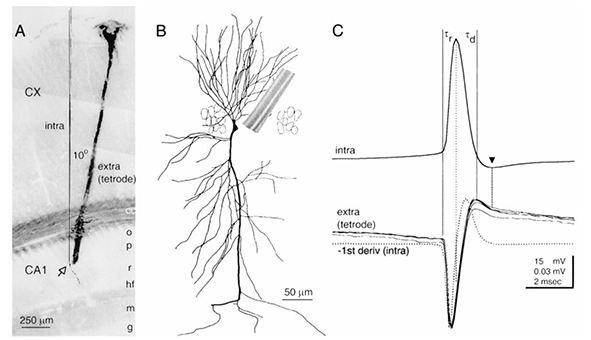
\includegraphics{Figures/Spikes/Spikes-Henze-w100-r150}
\end{center}
\caption[Intracellular and extracellular action potentials]{\textbf{Simultaneous recording of intracellular and extracellular action potentials (`spikes').}
Adapted from \citeasnoun**{Henze2000}.
\gen{Figure + caption to be updated}
}
\label{fig:Spikes:Henze}
\end{figure}
%%%%%%%%%%%

While the amplitude of the membrane-potential deflection during an action potential is about 100~mV, the amplitudes of spikes are typically less than 1~mV. 
Also, the shape of the spike is very different from the shape of intracellularly recorded action potentials (\Fref{fig:Spikes:Henze}).
The initial sharp negative peak is often referred to as the `sodium peak' as it mainly stems from sodium ions flowing into the soma (and axon hillock)
during the initial phase of the action potential. The latter blunter positive peak is likewise sometimes referred to as the `potassium peak' as 
it is dominated by potassium ions flowing out of the soma. \gen{Dette maa vel vaere riktig aa si?}

When detecting spikes, the main issue is that the spike amplitude is larger than the ambient noise level, typically some tens of $\mu$V. 
%\gen{Har vi et godt tall med medhoerende referanse her?} 
%\ehnote{Tja. Ambient noise er jo veldig avhengig av forskjellige faktorer, elektrode-type og impedans, in vivo vs. in vitro, vaaken vs. bedoevet tilstand osv, valg av filter, osv.}
%\tvnnote{Alessio sa de typisk ikke tar med spikes med amplitude under 30 uV, og det var dette vi brukte i Buccino et al., 2018, J Neurophysiol, men han hadde ikke noe god kilde ellers}
For the detection of spikes, the detailed spike shape is of less importance. However, an extracellular electrode will in general measure spikes from several neurons positioned in the vicinity of the electrode contact. To obtain spike trains from individual neurons, the recorded spikes must thus be sorted in a process referred to as spike sorting~\cite**{Quiroga2007}. And in this process, the differences in spike shapes are crucial~\cite**{Einevoll2012}. 
Spikes shapes are also used to distinguish spikes from different neuron types. The temporal width of the spike is, for example, used to separate putative inhibitory neurons (narrow spikes) from excitatory neurons (broad spikes). But a more detailed separation into subgroups is also possible~\cite**{Buccino2018}.

Detailed modeling of spikes are important for several reasons: for example, 
(i) to understand what the single-neuron properties can tell us about spike shapes (and the other way around) \cite**{Holt1999,Gold2006,Pettersen2008a,Anastassiou2013},
(ii) to estimate biases regarding which types of neurons preferentially generate the spikes recorded by electrodes \cite**{Pettersen2008a},
(iii) to provide benchmarking data for development and testing of methods for spike sorting or spike-based neuron identification \cite**{Einevoll2012,CamunasMesa2013,Hagen2015,MondragonGonzalez2017,Buccino2020}, and (iv) to fit model parameters in multicompartment neuron models \cite**{Gold2007}.

%%%
\section{\blue{Recording of spikes}}
\label{sec:Spikes:recording}
Spike recordings are typically done in living brains. Here the signal is obtained by high-pass filtering the extracellular potentials, with a lower cut-off set at some hundred hertz.
In contrast, the low-frequency part, the local field potential (LFP), is thought to mostly reflect synaptic inputs onto populations neurons around the contact~\cite**{Einevoll2013},
see \Fref{chap:LFP}.

A common misunderstanding is that a spike is built up only of high-frequency components.
The reasoning is that a spike typically lasts only a couple of milliseconds and an oscillation with a period of, say, 
2 milliseconds corresponds to a frequency of 500 hertz, lower frequencies will be absent or at least very weak.
But this is not generally true~\cite**{Pettersen2008,Schomburg2012,Ray2011,Scheffer-Teixeira2013}. 
Even a fast sodium spike contain frequency components with frequencies as low as 100 Hz \cite**{Pettersen2008a}.
This is illustrated in Figure~\Fref{fig:Spikes:freq_dep} showing that also very narrow spikes may contain low-frequency components.
In fact, a so-called $\delta$-function pulse which essentially is infinitely sharp and 
has zero width, is built up of equal amounts of frequency components for all frequencies.
And slower phenomena such as calcium spikes~\cite**{Stuart2007}, spike afterhyperpolarization \cite**{Buzsaki1988}, and strongly correlated action-potential firing \cite**{Schomburg2012}
may further contribute to increased low-frequency components~\cite**{Buzsaki2012}. 

%%%%%%%%%
% Figure
%%%%%%%%%
\begin{figure}[!ht]
\begin{center}
%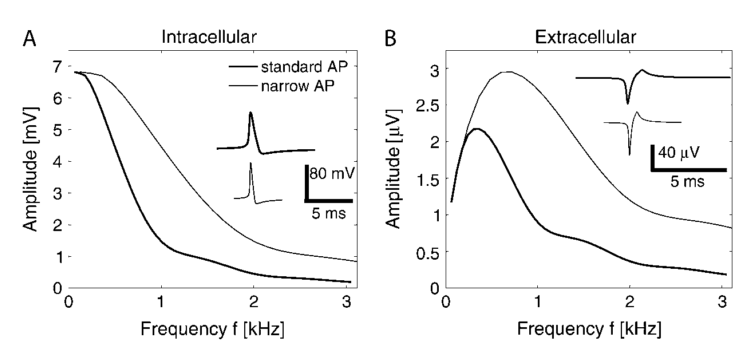
\includegraphics[width=0.6\textwidth]{Figures/Spikes/Spikes-eap_illustration.png}
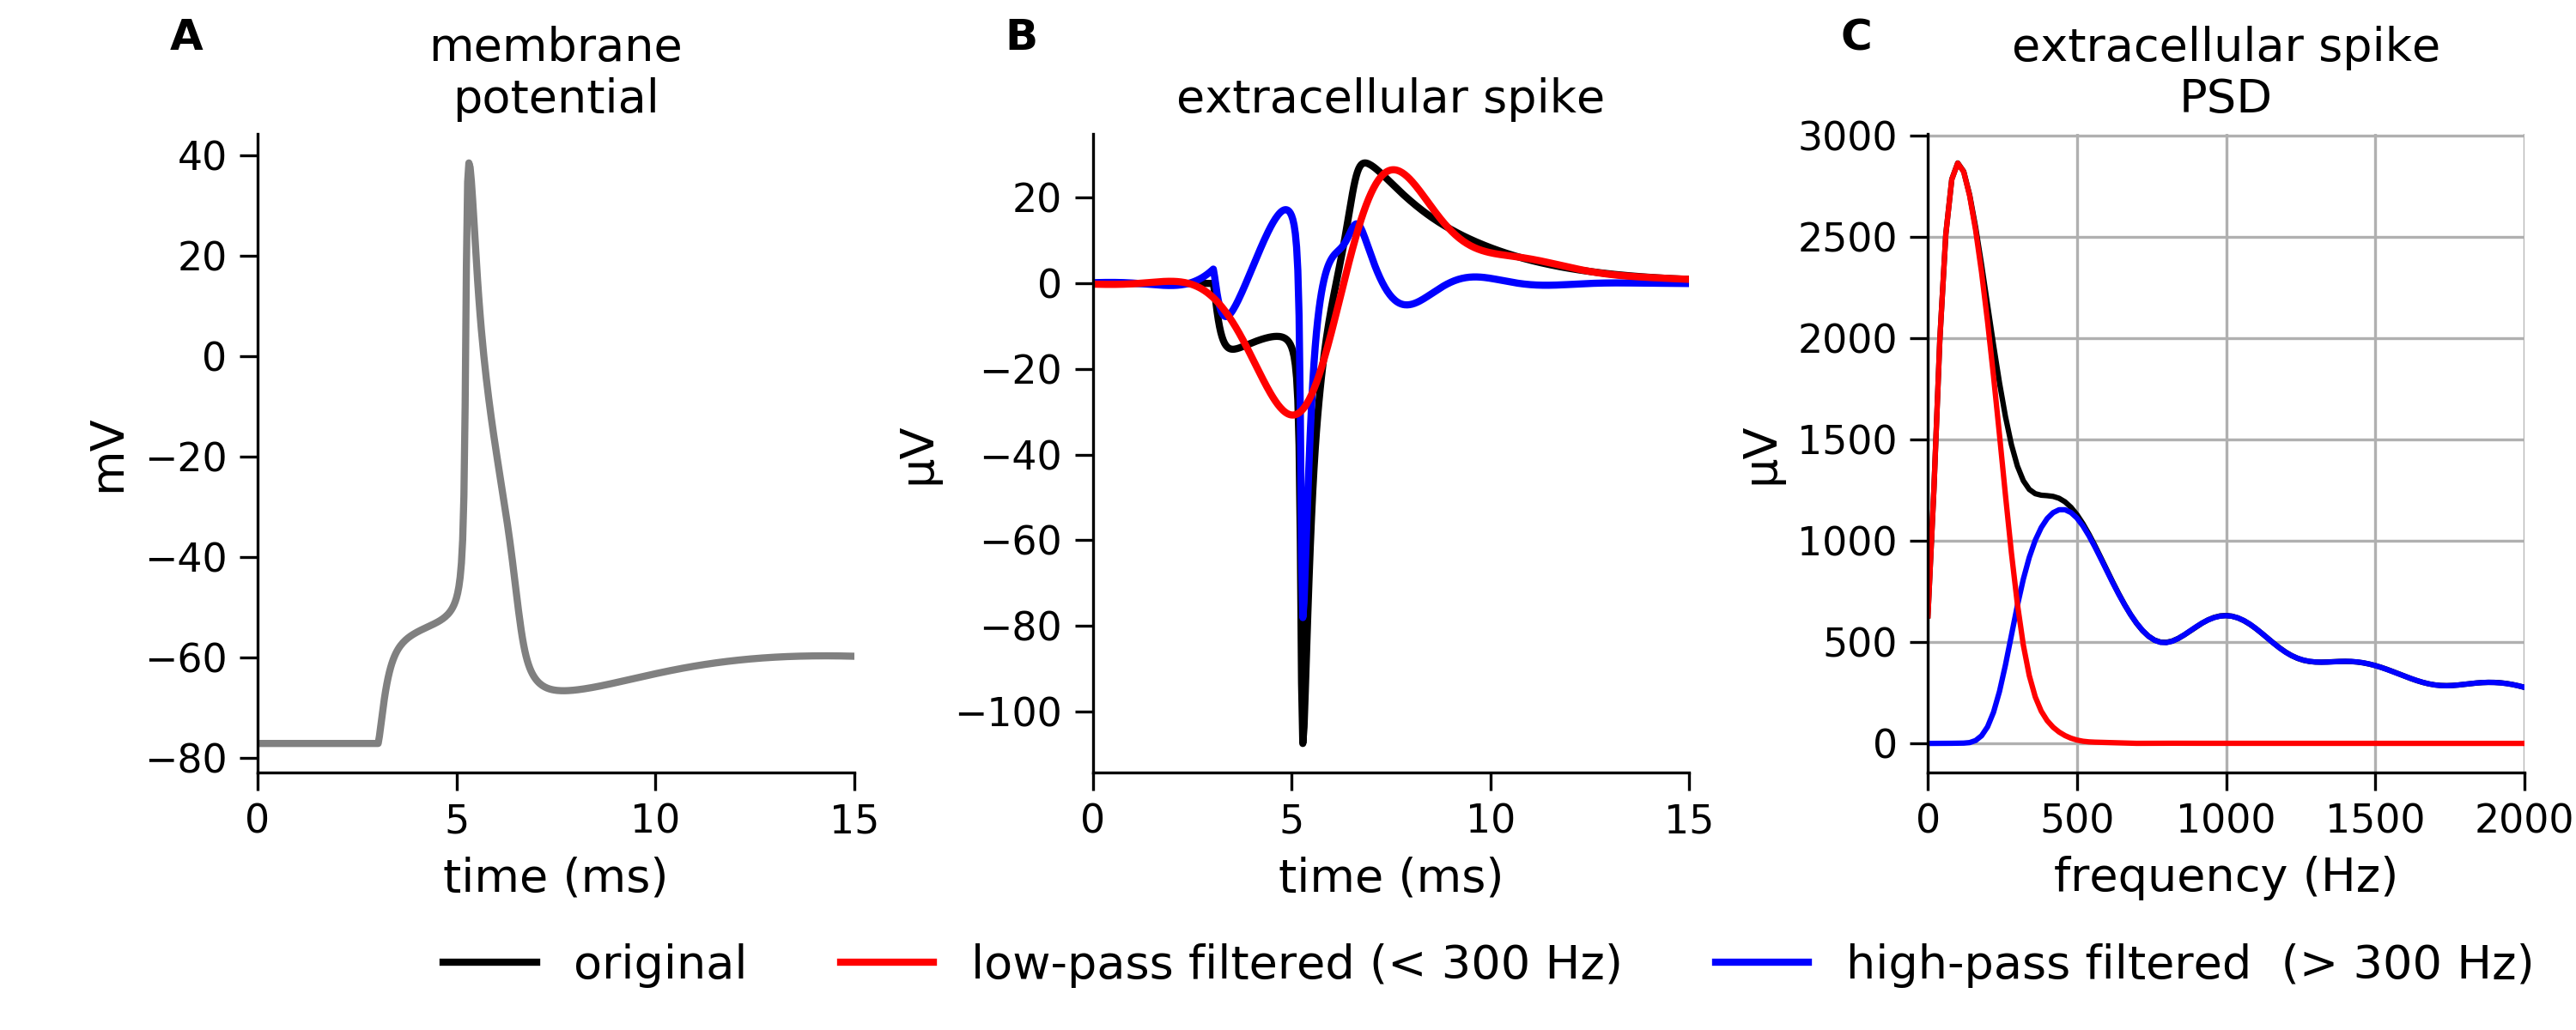
\includegraphics[width=1.0\textwidth]{Figures/Spikes/Spikes-fig_spike_freq_content_amp.png}
\end{center}
\caption{\textbf{Spike and frequency components.}
A: Membrane potential during firing of action potential of Hay neuron~(\gex{REF}) %\cite**{Hay2011}.
B: Corresponding extracellular spike measured \gex{XX $\mu$m} outside of soma neurons. Raw signal (black),
low-pass filtered signal (red), high-pass filtered signal (blue).
C: Frequency content of signals in B, that is, amplitudes for frequency components found by Fourier transformation.
\gen{Kanskje vi kunne legge til Fourier spektrum for intracellular action potentials ogsaa slik at vi kan kommentere
at ikke bare spike-formen i tid, men ogsaa i frekvens, er veldig forskjellig?}
\gen{Enhet paa y-akse i C maa fikses. Tar vel ogsaa bort bakgrunns-rutegrid i C?}  
}
\label{fig:Spikes:freq_dep}
\end{figure}
%%%%%

%%%%%%%%%
% Figure
%%%%%%%%%
\begin{figure}[!ht]
\begin{center}
%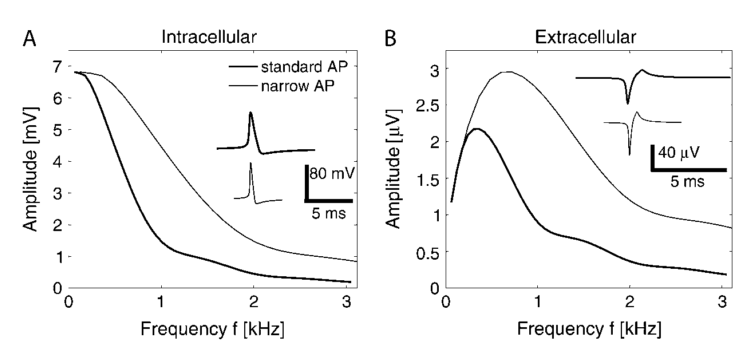
\includegraphics[width=0.6\textwidth]{Figures/Spikes/Spikes-eap_illustration.png}
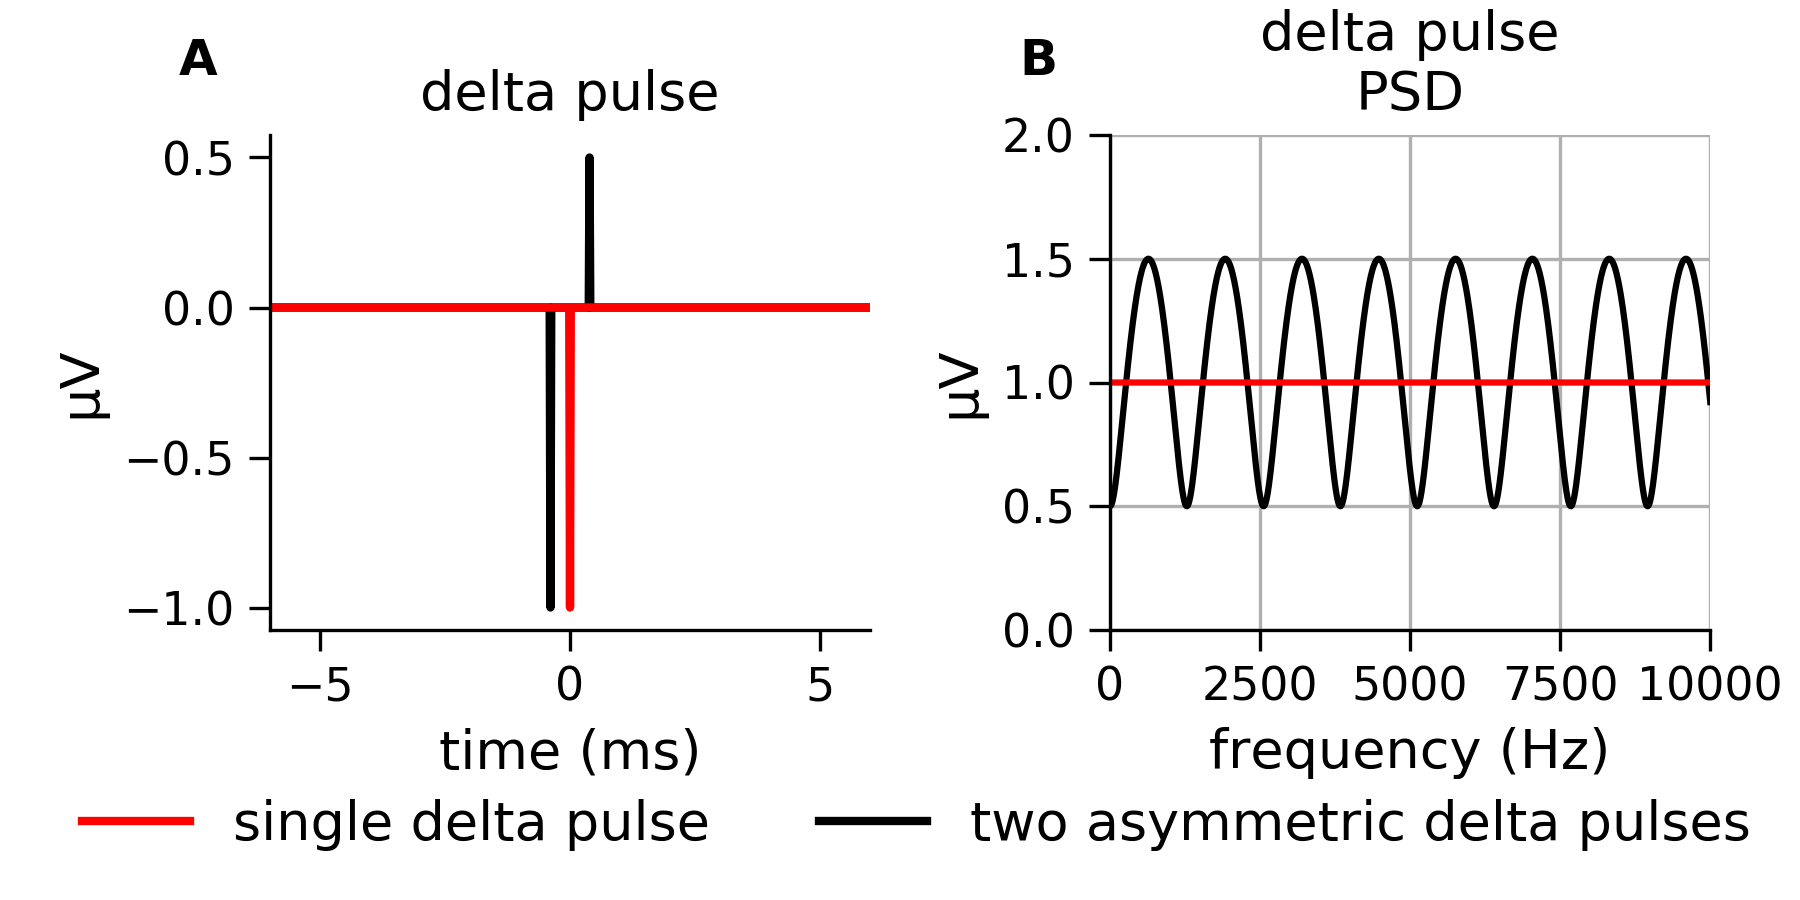
\includegraphics[width=1.0\textwidth]{Figures/Spikes/Spikes-fig_delta_pulse_freq_content.png}
\end{center}
\caption{\textbf{Delta pulses and frequency content.}
A single delta-pulse (panel A, red) has frequency components with equal contributions for all frequencies (panel B, red).
An asymmetric pair of delta-pulses, caricaturing the spike in \Fref{fig:Spikes:freq_dep}B with a negative sodium peak followed by a weaker
positive potassium peak (panel A, black), instead has an oscillating frequency spectrum (panel B, black). This spectrum has its (first) maximum at 
625 Hz, but also has substantial contributions from frequencies all the way down to zero.
\gen{Kanskje la x-aksen faa fra 0 till 2000 Hz som i Fig. 8.2B? Tar vel ogsaa bort bakgrunns-rutegrid i B? Enhet paa y-akse i B maa fikses.
Kanskje vi kan velge -100 $mu$V som amplitude paa sodium-pulse i A slik at det ligner mer paa  Fig. 8.2?}
}
\label{fig:Spikes:freq_dep_delta}
\end{figure}
%%%

The high-pass filtering of the extracellular signal typically used in extraction of spikes from extracellular recordings, 
changes the shape and reduces the signal power of the extracellular spike signal.  The rationale for this high-pass filtering is 
not to modify the spike shape and make it more amenable for detection or spike sorting. It is rather to remove the low-frequency (LFP) part which
stems from the other slower neural processes.  This LFP signal typically dominates in terms of overall power, but has very little power above a few hundred hertz~\cite**{Pettersen2008,Einevoll2013}.

Overviews over the challenges when measuring spikes can be found in  \citeasnoun**{Anastassiou2013} and \citeasnoun**{Whittingstall2013}.
\gen{Noen andre mulige referanser her?} 

 %%%%%%%%%%
% Figure: Spike from multi-compartment model
%%%%%%%%%%
%\begin{cnfigure}{Figures/mm/EP-spike-MultiCompartment-w100-r150}
\begin{figure}[!ht]
\begin{center}
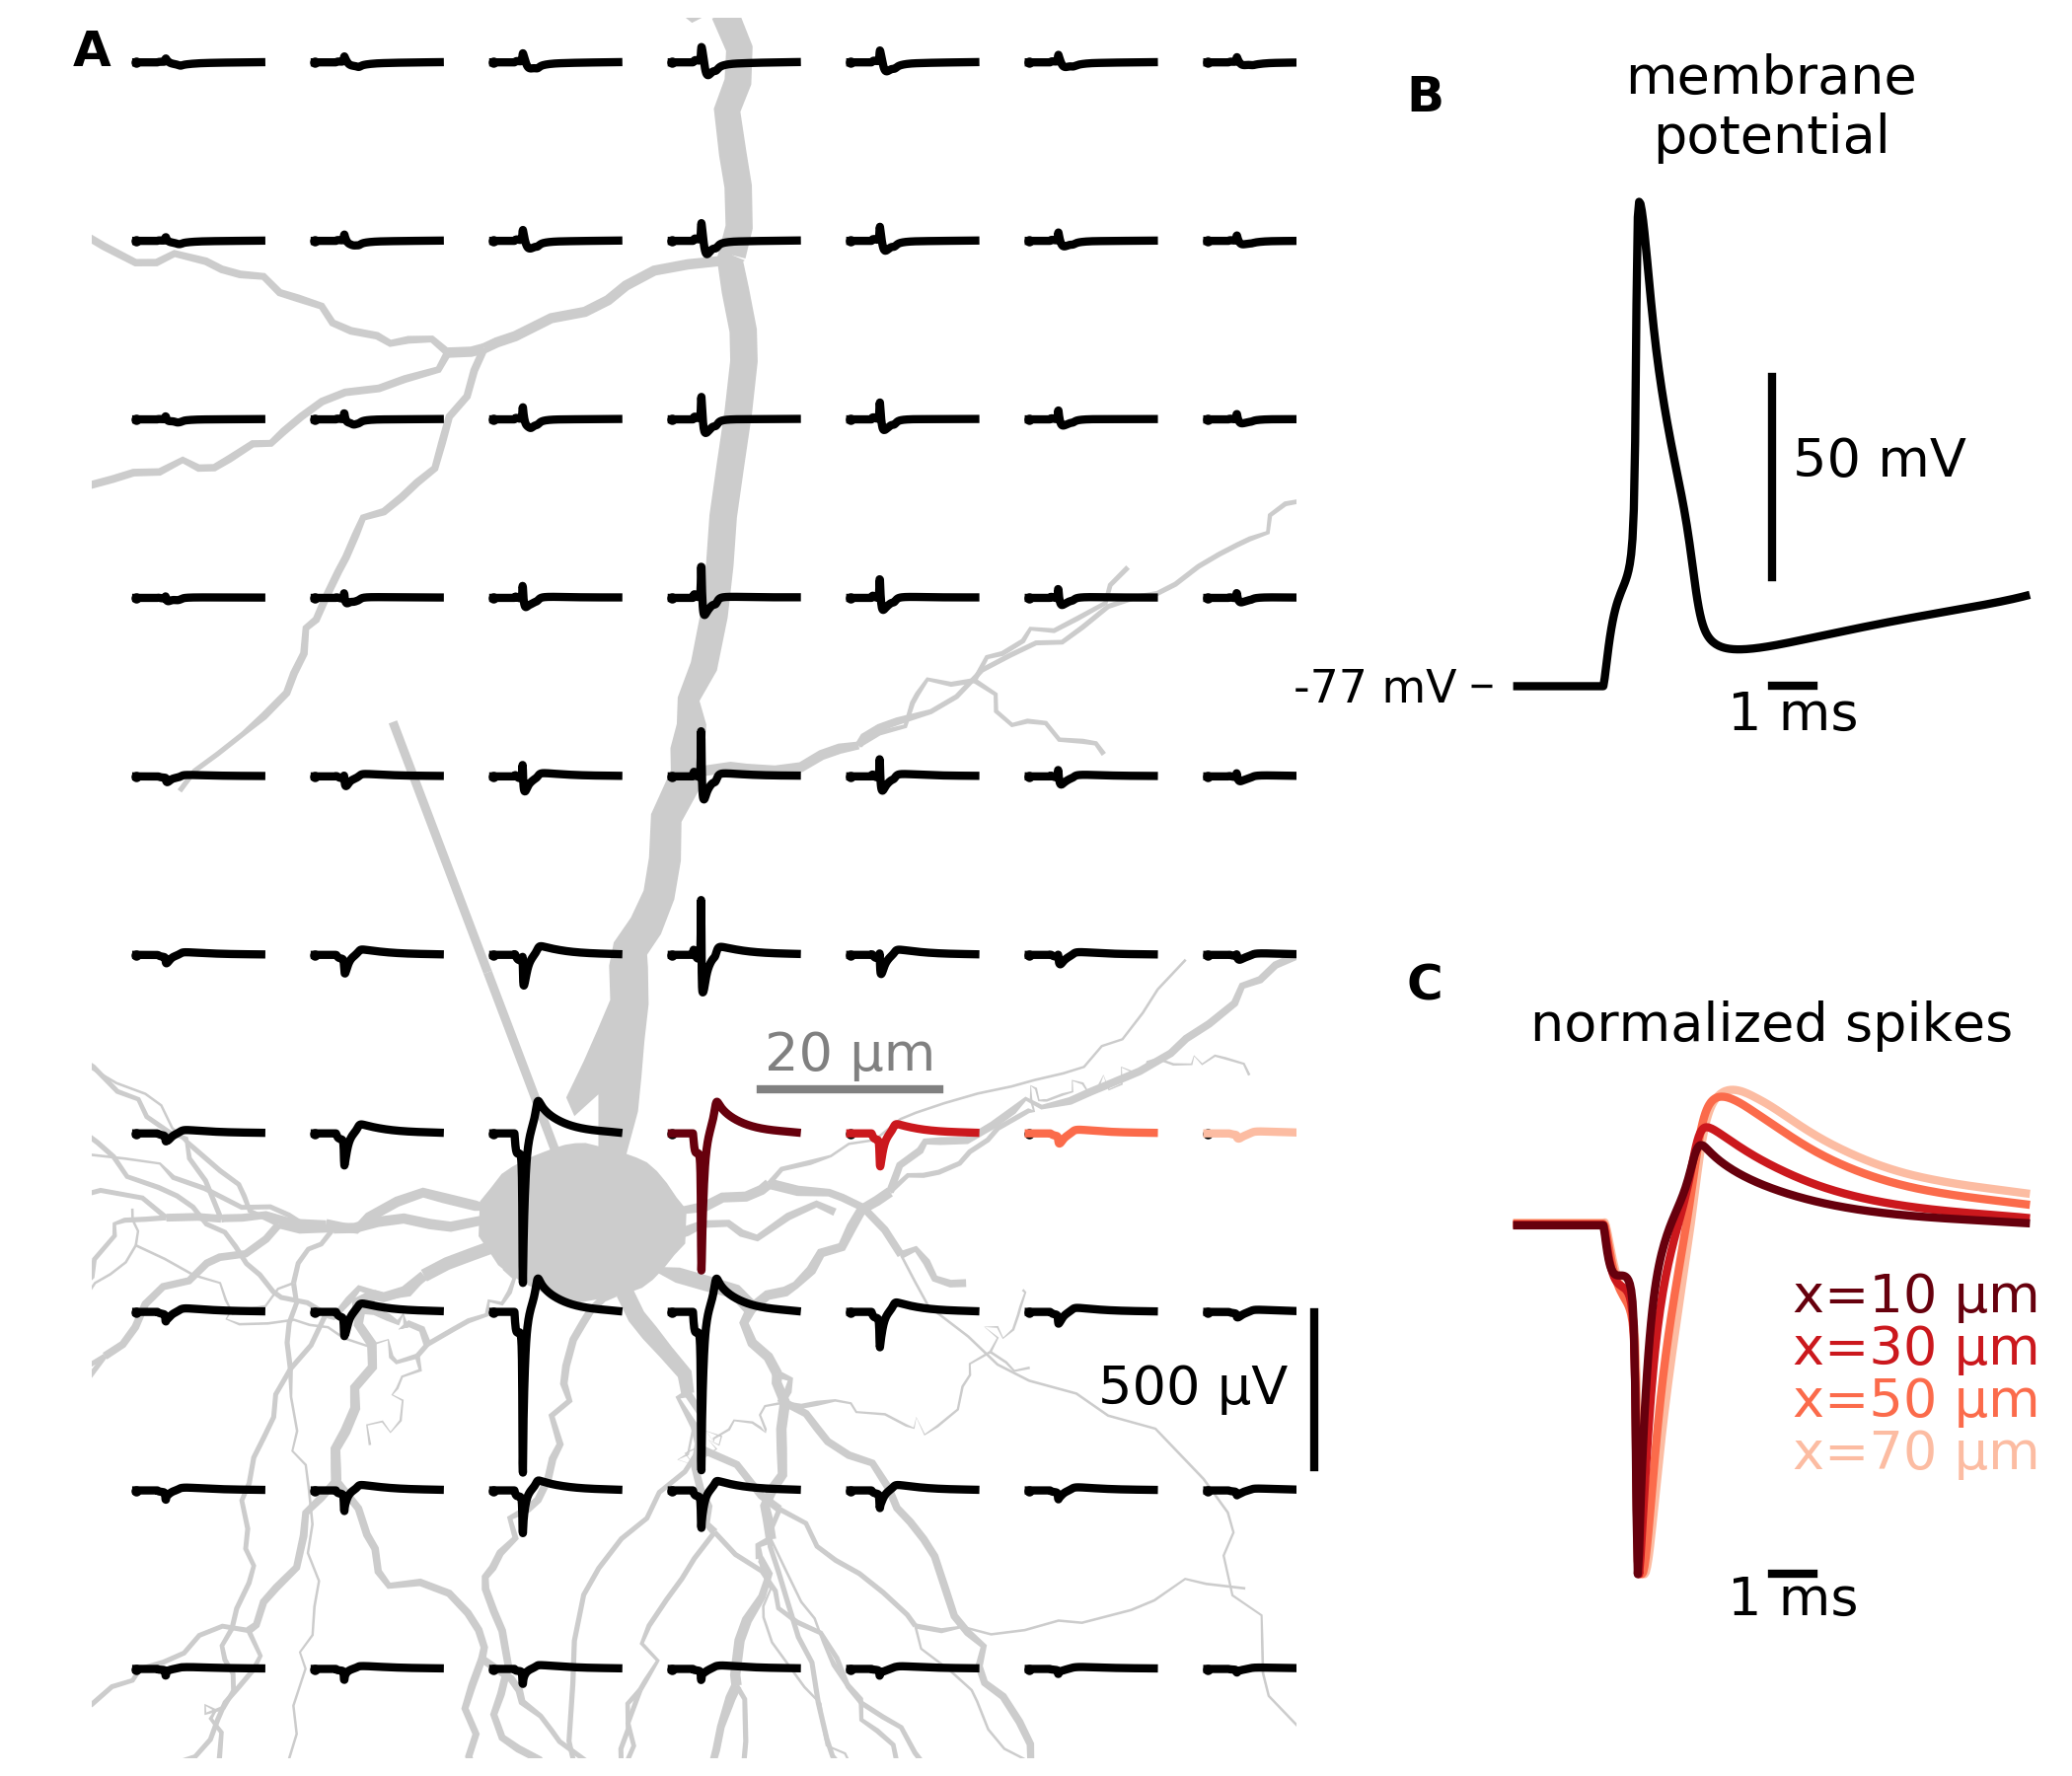
\includegraphics[width=1.0\textwidth]{Figures/Spikes/Spikes-fig_hay_eap_simpler}
\end{center}
\caption[]{\textbf{Spike from action potential for a multi-compartmental neuron model.}
A: Spikes computed at different positions around example Hay-neuron \gex{(Ref. XX)} using \gex{Eq. XX}.
B: Corresponding membrane potential. C: Spike shapes at different lateral positions in A as depicted by colouring. Spike shapes
are normalized to have the same magnitude of the negative peak.
The action potential was generated by injection of synaptic currents into the soma of the model neuron. 
\ehnote{Figure adapted from Fig4. i Hagen2015 kanskje? Aksonet peker i "feil" retning ogsaa. 
Det boer nevnes hva som driver depolariseringen, ser ut som en step current?}
\tvnnote{Vi ville ha en litt enklere versjon enn Fig. 4 i Hagen2015, men enig i at vi kanskje boer vurdere aa fikse retningen til axonet. Har du koden for dette? Stimuli er foreloebig synaptisk input i soma}
}. 
%Active sodium
%and potassium conductances in the soma compartment and computed from 
%\Fref{XX:equation:Ve-multi-compartment}.
%Left panel shows the EP at different spatial positions, while right panel shows the corresponding
%soma membrane potential during the action potential. 
%\gen{Figure + caption to be updated. Change to Hay-model,}
\label{fig:Spikes:MultiCompartment}
%\figpermOurs
\end{figure}

%%%
\section{\blue{Spikes from multi-compartment neuron models}}
\label{sec:Spikes:multi-compartment}
%%%
Unlike the intracellular somatic action potential which has a quite standardized appearance, the spike shapes and amplitudes can vary
strongly depending on the position at which it is recorded.  This is illustrated in \Fref{fig:Spikes:MultiCompartment} showing computed spikes at various 
positions around a neuron during the firing of an action potential. 
Here the scheme described in Chapter \gex{XX} is used with a biophysically detailed neuron model for a layer-5 pyramidal cell.
One striking features is the rapid decay of spike amplitude with distance from the soma. Another is the changing shape of the spike
highlighted in panel C: The sharpest spikes are seen for recording close to the soma. This blunting, or low-pass filtering, of the spike with distance stems from
the cable properties of the neuron, and has been referred to as `intrinsic dendritic filtering' \cite**{Linden2010,Pettersen2012} 
(as opposed to, say, possible filtering by the extracellular medium itself~\cite**{Bedard2012}). 
The origin of this intrinsic dendritic filtering effect is described below in \Fref{sec:Spikes:ball-and-stick}.

%A more detailed picture of spike shapes is obtained by considering a detailed multi-compartmental neuron model
%with a comprehensive branching structure typical for real neurons as in Figure~\Fref{fig:Spikes:MultiCompartment}.
%With this dendritic morphology the membrane currents through the dendrites are spread over a larger membrane area.
%As a result, \Fref{XX:equation:Ve-multi-compartment} predicts that the largest EP spikes will be seen
%around the soma for the example pyramidal neuron in Figure~\Fref{fig:Spikes:MultiCompartment}.  
%Around the apical dendrites, the spikes will still have an inverted shape compared to spikes close to the soma. 
%However, their amplitudes will be small, only a few microvolts, so they will not be seen in most experiments.
%
%As for the two-compartment spike model, the spike amplitude in Figure~\Fref{fig:Spikes:MultiCompartment} 
%decays sharply with distance from the neuron. In addition, the spike width increases
%with distance as demonstrated by the insets at two example positions. For the large spike recorded next to
%the soma the half-width of the spike is $\sim$0.6~ms, while at the position outside the dendrite, the half-width is increased to
%$\sim$0.7~ms. This corresponds to a low-pass filtering in the sense that the distant EP has lost some 
%high-frequency components compared to the EP close to the soma. This filtering effect is absent for the spike generated by the 
%two-compartment neuron model, and reflects that the cable properties of dendrites are important in determining 
%also the shape of recorded spikes.   
%
%*******




%%%
\section{\blue{Spikes from two-compartment neuron model}}
\label{sec:Spikes:two-compartment}
%%%
To what extent can the qualitative features regarding the position dependence of spikes seen 
in \Fref{fig:Spikes:MultiCompartment} be explained by simpler neuron models? 
While intracellularly recorded action potentials can be modelled with a single-compartment neuron model, 
the two-compartment model model is the simplest neuron model that can provide an extracellular spike at all. 
An example of a spike generated by such a model is shown in Figure~\Fref{fig:Spikes:DifferentNeuronModels}D. Around the soma, characteristic
spikes with a sharp negative peak followed by a slower positive hump is seen, in accordance with typical experimental
spike recordings as exemplified in Figure~\Fref{fig:Spikes:Henze}. The same spikes with inverted form are observed outside
the dendrite compartment. Such inverted spikes are rarely, if ever, seen in experiments, however. This suggests that while the two-compartment model can account for large spikes recorded next to the soma, it is inadequate for 
predictions of  the detailed spatial pattern of spike shapes that would be recorded by an electrode at different positions around a neuron.   

Spike amplitudes in the two-compartment model are seen to decay with distance as in the multi-compartment model. However, the two-compartment predictions differ in that the spike shape (panel D, bottom) do not depend on position (except for possibly a complete inversion). 
This can be readily understood from the two-compartment cable equation circuit \gen{Synes vi boer gaa gjennom denne modellen et sted i teorien slik at vi kan
refere til den her ...}. The transmembrane current (including the capacitive current) that enters the soma compartment must at all times equal the transmembrane current leaving the dendrite compartment. The spike will thus be set up by the sum of two monopolar contributions with the same magnitude and opposite signs, and the only feature that will vary with spike position is the net amplitude of the spike. The shape of the spike will always be the same.

     

%%%%%%%%%%
% Figure: Spikes from two-compartment, ball-and-stick and multicompartment
%%%%%%%%%%
%\begin{cnfigure}{Figures/mm/EP-spike-TwoCompartment-w100-r150}
\begin{figure}[!ht]
\begin{center}
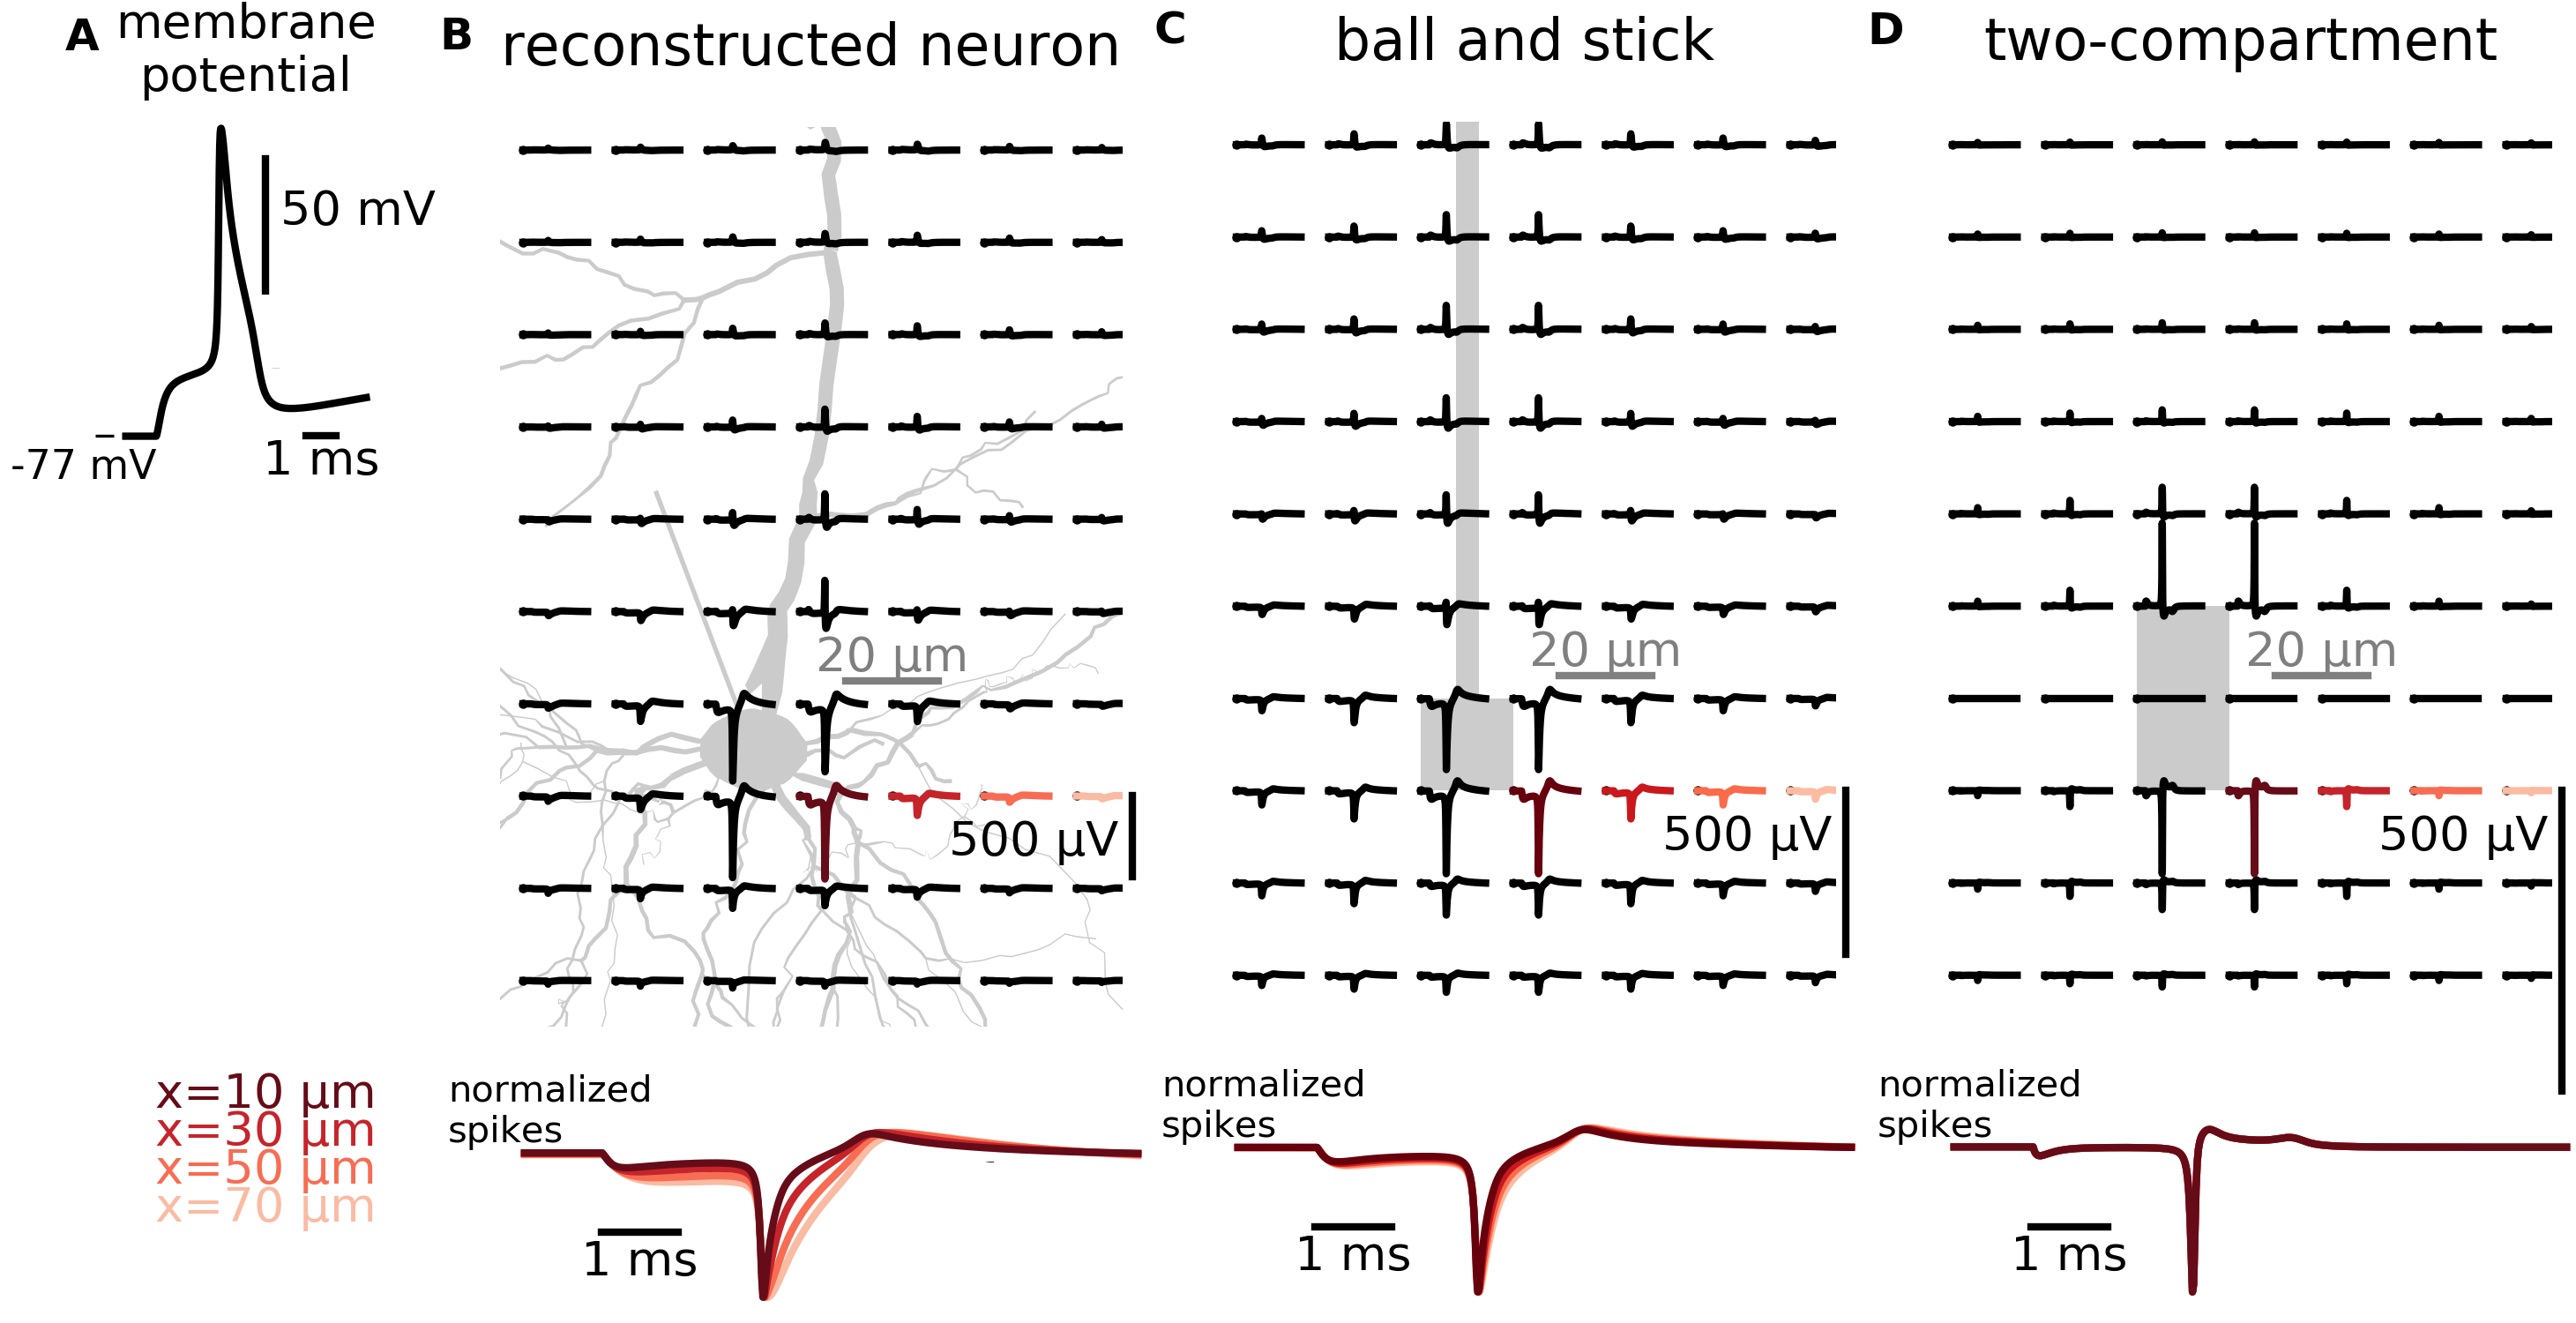
\includegraphics[width=1.2\textwidth]{Figures/Spikes/Spikes-compare_hay_bns_2c_reformat_2}
\end{center}
\caption{\textbf{Comparison of spikes from action potential for different neuron models.}
A: Membrane potential during spiking event, generated by injection of synaptic current into the soma of  example Hay-neuron \gex{(Ref. XX)}.
B: Spikes computed at different positions around example Hay-neuron using \gex{Eq. XX} (top). 
C: Spikes computed for example ball-and-stick neuron when imposing the membrane potential in A in the soma of the model neuron (top). 
Neuron parameters are \gex{XX}. 
D: Spikes computed for example two-compartment neuron when imposing the membrane potential in A in the soma of the model neuron (top). 
Neuron parameters are \gex{XX}. 
For panels B--D, spikes shapes at different lateral positions as depicted by colouring, are shown in bottom panels. Spike shapes
are normalized to have the same magnitude of the negative peak.
\gen{Lurer paa om panelene kunne blitt finere ved aa bruke et kortere utsnitt langs tidsaksen?}
}
\label{fig:Spikes:DifferentNeuronModels}
\end{figure}

%%%
\section{\blue{Spikes from ball-and-stick neuron}}
\label{sec:Spikes:ball-and-stick}

Unlike the two-compartment neuron model, the so-called ball-and-stick neuron model exhibits position dependence of the spike shape
(\Fref{fig:Spikes:DifferentNeuronModels}C). In this model a dendrite cable `stick' is connected to a point-like soma.
The effect is not as pronounced as for the anatomically detailed multi-compartment neuron model (panel B),
but the key qualitative feature remains: the spike gets blunter when moving away from the soma.
In particular, the width of the negative sodium peak is seen to increase with increased lateral distance.

Unlike multi-compartment neuron models, the ball-and-stick neuron is amenable to analytical mathematical studies. 
\citeasnoun**{Pettersen2008a} took advantage of this and used this model to explore the link between the morphology and electrical properties of 
neurons and the shape and size of the spike it produces during an action potential. 
Figure~\Fref{fig:Spikes:ball-and-stick-results} shows the distance dependence of the spike amplitude and spike width both for a detailed multi-compartmental pyramidal neuron model and ball-and-stick neurons.
While the spike width and amplitude of the multi-compartmental neuron are larger than for
the two example ball-and-stick neurons (with short and long dendrite sticks, respectively), 
the shapes of the curves are similar. \ghnote{Kan vi ikke velge parametere slik at amplituden og shapen ligner i de to tilfellene?} 
\gen{Jo, det kan sikkert vaere mulig. Dette er klippet rett fra Pettersen2008a.}
Note also that the results for a ball-and-stick neuron with an infinitely long dendritic stick is
effectively identical to the long-stick results in the figure~\cite**{Pettersen2008}.


%%%%%%%%%%
% Figure: Spike widths and amplitudes
%%%%%%%%%%
%\begin{cnfigure}{Figures/mm/EP-spike-ball-and-stick-results-w100-r150}
\begin{figure}[!ht]
\begin{center}
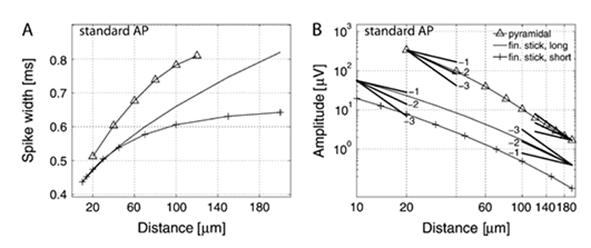
\includegraphics{Figures/Spikes/Spikes-ball-and-stick-results-w100-r150}
\end{center}
\caption[]{
Spike widths (left) and (peak-to-peak) spike amplitudes (right) as a function of
distance from soma for a detailed pyramidal cell model (pyramidal) and two
types of ball-and-stick models: long, finite ball-and-stick
model (fin.~stick, long) with diameter $d=2~\mu$m and length
$l=1$~mm and a short, finite ball-and-stick model (fin.~stick, short) with diameter $d=1~\mu$m and length $l=0.2$~mm.
The intracellular action potential shown in the inset in the left panel of 
\Fref{fig:Spikes:ball-and-stick-frequency} was imposed as a voltage-clamp in the soma,
and the size and electrical properties of the soma thus did not affect the results.
The EP was recorded in the
somatic plane normal to the stick/primary apical dendrite. 
In right panels guidelines illustrating the power-law decays $1/r$ and
$1/r^{2}$ have been added. 
For further details see \citeasnoun[Figure 6]{Pettersen2008}.
\gen{Figure + caption to be updated.} 
Adapted from \citeasnoun**{Pettersen2008}. 
\gen{Her kunne man jo kjoert ut nye resultater for Hay-modellen, men det er vel like greit aa bare bruke figurene fra 
Pettersen2008?} \tvnnote{Gaar jo forsaavidt fort aa lage paa nytt, og kan jo vaere fint at det blir en del av koden leserne har tilgjengelig?}
\gen{Enig. I tilfelle maa ogsaa Fig. 8.7 lages paa nytt.} 
}
\label{fig:Spikes:ball-and-stick-results}
%\figpermOurs
\end{figure}
%%%%


%
%%%%%%%%%%%
%% Figure: Neuron models considered in plot of spike widths and amplitudes
%%%%%%%%%%% 
%%\begin{cnfigure}{Figures/mm/EP-spike-ball-and-stick-neuron-models-w43-r300}
%\begin{figure}[!ht]
%\begin{center}
%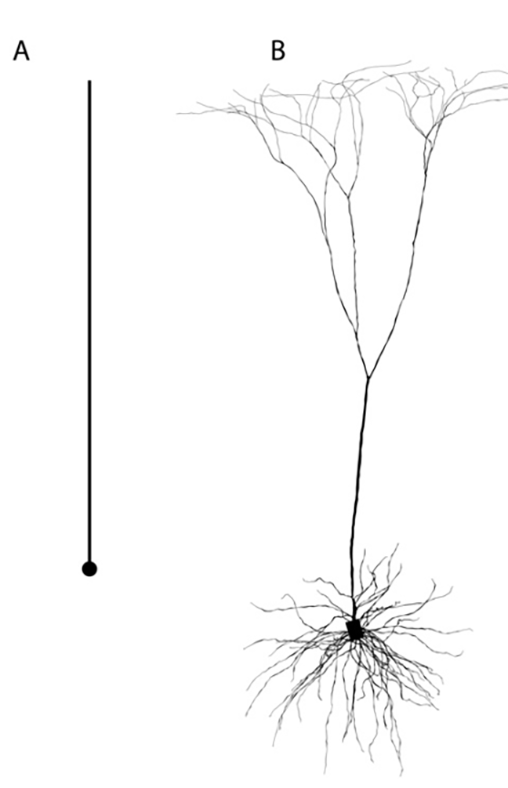
\includegraphics{Figures/Spikes/Spikes-ball-and-stick-neuron-models-w43-r300}
%\end{center}
%\caption[]{\textbf{Neuron models considered in results in Figure~\Fref{fig:Spikes:ball-and-stick-results}}. 
%\gen{Mulig vi ikke trenger en slik figur lenger pga Fig 8.3}
%Adapted from \citeasnoun**{Pettersen2008}.
%}
%\label{fig:Spikes:ball-and-stick-neuron-models}
%%\figpermOurs
%\end{figure}

\subsection{\blue{Frequency components of spikes}}
\label{sec:Spikes:Fourier}

To understand the physical origin of these results it is easier to consider each frequency 
component of the action potential separately. From Fourier theory it follows that any signal
such as the time course of a spike $V_\mathrm{e}(t)$, can be written as a sum of waves with different frequencies.
Such a Fourier sum can be constructed in various ways. The derivations presented below 
building on \citeasnoun**{Pettersen2008a}, use the convention that a time signal $S(t)$ can be written as
%%%
\begin{equation}
S(t) = Re \{ \sum_{f}  \hat{S}(f) \exp (j 2 \pi f t) \}
\label{eq:Spikes:Fourier_sum}
\end{equation}
%%%
where $Re\{z\}$ represents the real part of the complex number $z$.  
Here $j$ is the unit of imaginary numbers, $f$ is the frequency, and the weight $\hat{S}(f)$ is in general  
complex. 

Figure~\Fref{fig:Spikes:ball-and-stick-frequency} illustrates the Fourier decomposition of the
intracellular action potential (membrane potential) and extracellular spike, respectively.
In panel B the weight of the different frequency components needed to represent the signals are shown.
A key observation here is that unlike for the intracellular action potential, the largest
contributions to the extracellular spike, comes from frequencies larger than 100~hertz.
\ghnote{Det overrasket at f-spektrum til intra vs ekstra er saa fundamentalt ulike. Er signalet i Figurpanel A ufiltrert, mens det i B er filtrert?}
\gen{Nei, dette skyldes fysikken. Extra reflekterer transmembrane stroemmer som inneholder mer av de hoeye frekvensene enn det "lav-frekvente" membran-potensialet.}
\tvnnote{De er foroevrig betydelig likere i mine simuleringer med Hay modellen, selv om det generelle moensteret vel kanskje er omtrent det samme som her.}


%%%%%%%%%%
% Figure: Action potential and its frequency content
%%%%%%%%%%
%\begin{cnfigure}{Figures/mm/EP-spike-ball-and-stick-frequency-w90-r150}
\begin{figure}[!ht]
\begin{center}
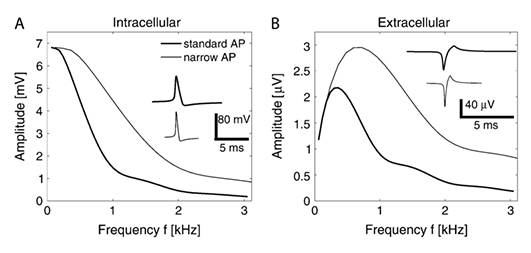
\includegraphics{Figures/Spikes/Spikes-ball-and-stick-frequency-w90-r150}
\end{center}
\caption[]{(a) Action potential used in simulations in Figure~\Fref{fig:Spikes:ball-and-stick-results}(inset) 
and its frequency content.
%The intracellular spike width is defined as the
%width of the AP at half amplitude and is 0.55~ms for the standard
%AP, and half the value for the narrow AP. 
(b) Frequency content of example extracellular spike.
Inset: Typical spike shape computed a distance $r=10~\mu$m
perpendicular to the dendrite at the level of soma for a ball-and-stick 
neuron with diameter $d=2~\mu$m and infinite dendrite length.
Here the intracellular action potential in left panel was imposed as a voltage-clamp in the soma.
The extracellular spike width is defined as the width of the negative phase at 25\% of its maximum
amplitude and is 0.44~ms for the example spike.
The amplitude (peak-to-peak value) of the spike is $56~\mu$V  
\gen{Figure + caption to be updated. Will only include standard AP in final figure.} 
Adapted from \citeasnoun**{Pettersen2008}.}
\gen{Her kunne man jo kjoert ut nye resultater for Hay-modellen, men det er kanskje like greit aa bare bruke figurene fra 
Pettersen2008?}
\label{fig:Spikes:ball-and-stick-frequency}
%\figpermOurs
\end{figure}

%\subsection{Frequency-dependent electrotonic length constant}
%\label{sec:Spikes:Fourier}
%
%For the ball-and-stick neuron, a membrane current entering the soma has to return to ECS through the cable stick, see Figure~\Fref{fig:Spikes:ball-and-stick-sketch}. When an oscillating membrane current is entered through the soma, the spatial pattern of return current will depend on the frequency of the oscillation due to the capacitive properties of the membrane: For higher frequencies the capacitive membrane current will be larger, and the 
%membrane effectively more leaky. Thus the injected soma current will return closer to the soma for higher frequencies, 
%as  seen in the inset in Figure~\Fref{fig:Spikes:ball-and-stick-sketch}.  

\subsection{\blue{Approximate spike formulas}}
\label{sec:Spikes:approximate}

To compute the extracellular spike generated by an imposed oscillatory current, the stick must be divided into small compartments  
and the multi-compartmental formula in Equation \gex{XX} used. 
This in general requires detailed knowledge of the resulting membrane currents in all compartments. 
While these can be computed for the ball-and-stick neuron (see, for example, \citeasnoun**{Pettersen2014}), 
the resulting formula for the spike becomes cumbersome and difficult to interpret.  
However, some useful insights can be obtained in two limiting cases: the recording being very near to the soma 
or very far from the soma.

%For recording positions very close to the soma, the contribution from the soma current will dominate 
%in the sum in \gex(XX). In this case the distance from the electrode
%to the return currents in the dendrite will be much larger than the distance to soma. 
%
%%
%With only the contribution from
%the soma compartment included, the amplitude $|\hat{V}_\mathrm{e,near}(f,\vec{r})|$  
%of the EP signal for each Fourier component with frequency $f$ is found to be

\subsubsection{Spikes recorded near the soma}
\label{sec:Spikes:near-spikes}
\tvnnote{En del bruker den deriverte av membranpotensial til aa approksimere spikes. Boer det taes med?}
\gen{Ja, det kommenteres naa lenger ned i "Spike shape dependence on distance".}
To understand the dependence of spike shapes and amplitudes on model parameters for the ball-and-stick neuron, it is useful
to consider the extracellular potentials set up by each of the frequency (Fourier) components of the action potentials separately. 
For recording positions $\vec{r}$ very close to the soma, the contribution from the soma current will dominate over the contributions from the dendrite 
in the sum giving the extracellular potential in Equation \gex{XX}. Then the amplitude of the
predicted oscillating extracellular potential $|\hat{V}_\mathrm{e,near}(f,\vec{r})|$ is approximately given by 
%
\begin{equation}
  |\hat{V}_\mathrm{e,near}(f,\vec{r})| = \frac{|\hat{I}_\mathrm{s}(f)|}{4 \pi \sigma r} 
  \label{eq:Spikes:Ve_near_1}
\end{equation}
%
where $|\hat{I}_\mathrm{s}(f)|$ is the amplitude of the oscillating current through the soma membrane.
%and also the axial current entering the dendrite from the soma compartment. 
For the relatively high frequencies of most relevance for the spike, this soma current is related to the soma membrane potential 
$\hat{V}_\mathrm{s}(f)$ through~\cite**{Pettersen2008a}
%
\begin{equation}
  |\hat{I}_\mathrm{s}(f)| =  \frac{\pi^{3/2} d^{3/2}}{\sqrt{2}} \sqrt{ \frac{f C_\mathrm{m}}{R_\mathrm{a}} }  |\hat{V}_\mathrm{s}(f)|
  \label{eq:Spikes:Isoma}
\end{equation}
%
and the contribution to the spike is thus found to be
%
\begin{equation}
  |\hat{V}_\mathrm{e,near}(f,\vec{r})| 
  = \frac{\sqrt{\pi}}{4 \sqrt{2} \sigma}
     \frac{d^{3/2}}{r} 
     \sqrt{ \frac{f C_\mathrm{m}}{R_\mathrm{a}} }  |\hat{V}_\mathrm{s}(f)| 
  \propto \frac{d^{3/2}}{r} \sqrt{ \frac{f C_\mathrm{m}}{R_\mathrm{a}} }  |\hat{V}_\mathrm{s}(f)| 
  \label{eq:Spikes:Ve_near_2}
\end{equation}
%
%%%%%%%%%%
%However, as shown in XX
%Box~\Fref{mm:box:ball-and-stick-spikes} 
%some useful insights can be obtained in two limiting cases: the recording being very near to the soma or very far from the soma.

%For recording positions very close to the soma, the contribution from the soma current will dominate 
%in the sum in \Fref{XX:equation:Ve-multi-compartment}. In this case the distance from the electrode
%to the return currents in the dendrite will be much larger than the distance to soma. With only the contribution from
%the soma compartment included, the amplitude $|\hat{V}_\mathrm{e,near}(f,\vec{r})|$  
%of the EP signal for each Fourier component with frequency $f$ is found to be
%%
%\begin{equation}
%  |\hat{V}_\mathrm{e,near}(f,\vec{r})| 
%  \propto \frac{d^{3/2}}{r} \sqrt{ \frac{f C_\mathrm{m}}{R_\mathrm{a}} }  |\hat{V}_\mathrm{s}(f)| 
%  \label{eq:Spikes:Ve_near}
%\end{equation}
%%
The suffix `near' is added because this expression only applies in the `near-field' limit, that is,
close to the soma.
$|\hat{V}_\mathrm{s}(f)|$ is the amplitude of Fourier component of the soma membrane potential at the same
frequency (see Figure~\Fref{fig:Spikes:ball-and-stick-frequency}). Further, $d$ is the diameter of the dendritic
stick, $C_\mathrm{m}$ is the specific membrane capacitance, and $R_\mathrm{a}$ is the specific axial resistance.  

%One of the predictions from the formula in \Fref{eq:Spikes:Ve_near_2} is that the amplitude of each Fourier component decays
%as $1/r$ when moving away from soma (yet staying within distances where the `near-field' approximation is still applicable).
%Since this applies to all Fourier components which together constitute the action potential, this implies that the amplitude of the 
%spike will decay as $1/r$ in this regime as well.
%\gen{From David Sterratt: Intuition for the relationship witd $d, C_m, f, r_a$.}

%%%%%%%%%%
% Figure: Frequency-dependent distribution of return currents
%%%%%%%%%%
%\begin{cnfigure}{Figures/mm/EP-spike-ball-and-stick-sketch-w70-r300}
\begin{figure}[!ht]
\begin{center}
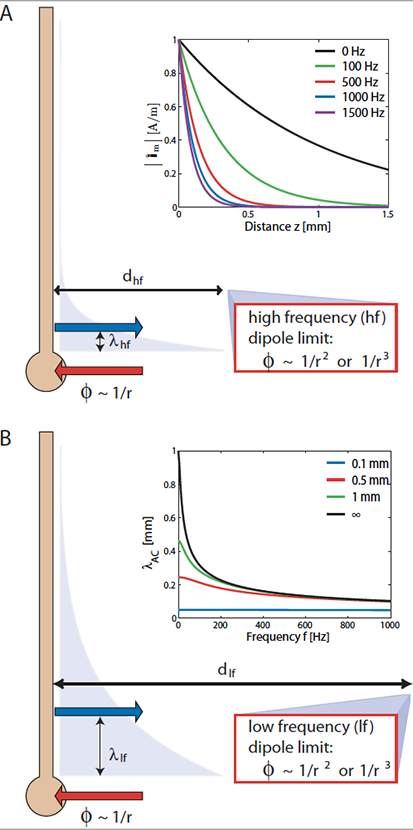
\includegraphics{Figures/Spikes/Spikes-ball-and-stick-sketch-w70-r150}
\end{center}
\caption[]{Illustration of ball-and-stick neuron and its frequency-dependent 
distribution of dendritic return currents following injection of a sinusoidal current into the soma.
The net current entering the soma will enter the dendrite as an axial current, and return to the 
ECS via the dendrite membrane. The inset shows the spatial distribution of this return current
for different frequencies. The higher the frequency, the closer the return currents will be and
the smaller the frequency-dependent length constant $\hat{\lambda}(f)$, reflecting the weighted mean 
of the return-current positions (see sidebox), will be. 
\gen{Figure + caption to be updated.} Adapted from \citeasnoun**{Pettersen2012}.
}
\label{fig:Spikes:ball-and-stick-sketch}
%\figpermOurs
\end{figure}
%


\subsubsection{Spikes recorded far away from soma}
\label{sec:Spikes:far-spikes}

For spikes recorded close to the soma, a single membrane current, the soma current,
dominates the sum in Equation \gex{XX}. 
For recording positions far away from the soma, the contribution from return membrane currents must also be included in the sum. For the ball-and-stick neuron, a membrane current entering the soma has to return to ECS through the cable stick, see Figure~\Fref{fig:Spikes:ball-and-stick-sketch}. When an oscillating membrane current enters through the soma, the spatial pattern of return current will depend on the frequency of the oscillation due to the capacitive properties of the membrane: For higher frequencies the capacitive membrane current will be larger, and the membrane effectively more leaky. Thus the injected soma current will return to the extracellular space 
closer to the soma for higher frequencies, as  seen in the inset in Figure~\Fref{fig:Spikes:ball-and-stick-sketch}.  

An approximate way of including the contribution to the spike from the dendritic return currents is to
assume all return currents to leave the dendrite at a single point on the dendrite. Then we are left with
a current dipole where the transmembrane current entering at the soma is at all times balanced by an oppositely directed current
with the same magnitude leaving at a single point on the dendrite. The current dipole length is then given by the distance
between the soma and the dendritic position of the return current. 

As shown in Figure~\Fref{fig:Spikes:ball-and-stick-sketch} this current dipole length will depend on frequency.
A natural choice is to choose the dipole length to be equal to the frequency-dependent length constant $\lambda_\mathrm{AC}(f)$ of the stick,
where the length constant corresponds to the mean value of the 
envelope of the sinusoidally varying (normalized) membrane current
$\hat{i}_\mathrm{m}$ weighted with distance $z$ from soma, see Figure~\Fref{fig:Spikes:ball-and-stick-sketch}. 
For an infinite dendrite stick this corresponds to
%
\begin{equation}
  \lambda_\mathrm{AC}^\infty(f) = \frac{\int_0^\infty z |\hat{i}_\mathrm{m}| dz}{\int_0^\infty |\hat{i}_\mathrm{m}| dz} 
  \label{eq:Spikes:formula_lambda_ac}
%=  \frac{\sqrt{2}\lambda}{\sqrt{\sqrt{W^2+1}+1}}.
\end{equation}
%
For high frequencies ($f \gg 1/2 \pi R_\mathrm{m} C_\mathrm{m}$) this is after some algebra 
found to give (see \citeasnoun[Appendix C]{Pettersen2008a} for details)
%
\begin{equation}
 \lambda_\mathrm{AC}^\infty(f) =  \frac{\lambda}{\sqrt{\pi f \tau}} = 
  \frac{1}{2\sqrt{\pi}} \sqrt{\frac{d}{f R_\mathrm{m} C_\mathrm{m}}}
\label{eq:Spikes:approx_lambda_ac}
\end{equation}
%
where $\lambda$ is the cable length constant from Equation~\gex{XX}.


Then the extracellular potential contribution from each frequency component can be approximated by using the 
dipolar expression in Equation~\gex{XX}, that is,
%%%
\begin{equation}
  |\hat{V}_\mathrm{e,far}(f,\vec{r})| =  \frac{|p(f) \cos \theta|}{4 \pi \sigma r^2} 
                                            = \frac{| \hat{I}_{s}(f) \lambda_\mathrm{AC}(f) \cos \theta|}{4 \pi \sigma r^2}   
                                                                                        \label{eq:Spikes:Ve_far_1}
\end{equation}
%Chapter~\Fref{XX:chap:XX}
Thus for spikes measured far away from the soma we find 
%  
\begin{equation}
  |\hat{V}_\mathrm{e,far}(f,\vec{r})|  = \frac{1}{8 \sqrt{2} \sigma} d^{2} \frac{1}{r^2  R_\mathrm{a}} 
      |\hat{V}_\mathrm{s}(f) \cos \theta | 
  \propto d^{2} \frac{|\cos \theta|}{r^2  R_\mathrm{a}} |\hat{V}_\mathrm{s}(f)| 
  \label{eq:Spikes:Ve_far_2}
\end{equation}
The suffix `far' is added because this expression only applies in the `far-field' limit, that is,
far away from the soma. 
%
%Equations~(\Fref{eq:Spikes:Ve_near_2}) and (\Fref{Spikes:box:equation:Ve_far_2}) describe how each frequency component of 
%the soma membrane potential  $\hat{V}_\mathrm{s}(f)$ is `translated' into frequency components of the 
%EP spike ($\hat{V}_\mathrm{e,near}(f,\vec{r})$ and $\hat{V}_\mathrm{e,far}(f,\vec{r})$, respectively). 
%%\end{boxfloat}
%%%%%%%%%%%%%%%%%%%%%%%%%%%%%%%%%%%%%%%%%


%An estimate of this length is provided by the 
%frequency-dependent length constant  $\lambda_\mathrm{AC}(f)$  corresponding to the weighted mean of the positions of the return currents along
%the dendrite stick (see Box XX). 
%Then with the use of expression for the EP around a current dipole in 
%\Fref{XX:equation:Ve-dipole-p}:
%%%%
%\begin{equation}
%  |\hat{V}_\mathrm{e,far}(f,\vec{r})|  \propto d^{2} \frac{|\cos \theta| }{r^2  R_\mathrm{a}}  |\hat{V}_\mathrm{s}(f)| 
%  \label{eq:Spikes:Ve_far}
%\end{equation}
%%%%



%A first observation from this formula is that the EP is no longer radially symmetric, and depends both on the radial distance $r$ from the neuron and  the angle $\theta$ with the dipole axis, that is, the direction of the dendritic stick.
%The amplitude will be largest above and below the neuron where $\theta=0^\circ$ and $\theta=180^\circ$, respectively. In the sideways direction 
%($\theta \sim 90^\circ$) the EP will be much smaller, as is characteristic for spatial pattern of potentials around a current
%dipole as illustrated in Figure~\Fref{fig:Spikes:TwoCompartment}. A qualitatively similar dipolar pattern, although not so distinct,
%is also seen for the spike generated by the biophysically detailed multi-compartment neuron in Figure~\Fref{fig:Spikes:DifferentNeuronModels}.


%Another difference of this far-field expression with the near-field expression in \Fref{eq:Spikes:Ve_near}, is that the
%amplitude decays as $1/r^2$, characteristic for potentials around dipolar sources, rather than $1/r$ which is characteristic for potentials around 
%a single source. This transition from a $1/r$ `monopolar' regime to a $1/r^2$ dipolar regime is indeed observed in
%the spike-amplitude panel in Figure~\Fref{fig:Spikes:ball-and-stick-results}.

\subsection{\blue{Spike amplitude dependence on distance}}
A prediction from the near-field formula in \Fref{eq:Spikes:Ve_near_2} is that the amplitude of each Fourier component decays as $1/r$ when moving away from the soma, 
as long as the position remains within distances where the `near-field' approximation still applies.
Since this applies to all frequency components which together constitute the action potential, this implies that the amplitude of the 
spike will decay as $1/r$ in this regime as well. 

Far away, the far-field formula \Fref{eq:Spikes:Ve_far_2} implies that the spike amplitude depends not only on the radial distance $r$ from the neuron, but also the angle $\theta$ with the dipole axis, the direction of the dendritic stick. The amplitude will be largest above and below the neuron where $\theta=0^\circ$ and $\theta=180^\circ$, respectively. In the sideways direction 
($\theta \sim 90^\circ$) the spike will be much smaller, as is characteristic for spatial patterns of potentials around a current
dipole as illustrated in Figure~\Fref{fig:Spikes:DifferentNeuronModels}D. A qualitatively similar dipolar pattern, although not so distinct,
is also seen for the spike generated by the biophysically detailed multi-compartment neuron in 
Figure~\Fref{fig:Spikes:DifferentNeuronModels}.
Another difference of this far-field expression with the near-field expression in \Fref{eq:Spikes:Ve_near_2}, is that the
amplitude decays as $1/r^2$, characteristic for potentials around dipolar sources, rather than $1/r$ which is characteristic for potentials around 
a single source. %This transition from a $1/r$ `monopolar' regime to a $1/r^2$ dipolar regime was also found in model studies with biophysically detailed 
%neurons \cite[Fig.~X]{Pettersen2008}.
%\todo{Connect to Figure :EP-spike-ball-and-stick-results}

An overall observation is that the spike is quite local, with the amplitude of the spike decaying rapidly with distance from the neuron soma. 
For the pyramidal neuron considered in Figure~XX, for example, the spike amplitude decays from about
300 microvolts a distance 20 micrometers from the soma centre to only about 10 microvolts a
distance 100 micrometers away. \gen{Update when new figures are added}
This rapid decay eases the interpretation of recorded spikes, since it implies
that in practice an electrode contact will only pick up spikes from neurons with somas positioned within a radius of some tens of micrometers.
%\todo{GTE: Rewrite this to compare with our own figure spikes around multicompartmental model + refer to Pettersen2008}  

%\paragraph{Spike amplitude dependence on neuronal parameters}
\subsection{\blue{Spike amplitude dependence on neuronal parameters}}
The spike amplitude is proportional to $d^{2}$ far away from the soma and to $d^{3/2}$ close to the soma,
where $d$ is the diameter of the dendritic stick diameter. This implies that far away from the soma the spike amplitude is proportional to  the cross-sectional area of the dendrite. Close to the soma, the spike amplitude also increases with dendrite diameter, but slightly less so.

Another observation is that the spike amplitude is independent of the membrane resistance $R_\mathrm{m}$ of the dendrite.
This reflects that the frequencies dominating the spike are so high that the ionic membrane current, governed by $R_\mathrm{m}$, is
much smaller than the capacitive membrane current, governed by membrane capacitance $C_\mathrm{m}$.  
Thus the spatial distribution of the return current along the dendrite will depend only on the capacitive current. This dependence
is seen through the presence of  $C_\mathrm{m}$ in the near-field formula in \Fref{eq:Spikes:Ve_far_2}. 
Note that in the far-field formula \Fref{eq:Spikes:Ve_far_2},  $C_\mathrm{m}$ is absent due to cancellation with another factor containing $C_\mathrm{m}$ in the mathematical derivation, 
cf. \citeasnoun[Equation 23]{Pettersen2008}.)

In Equations~\Fref{eq:Spikes:Ve_near_2} and \Fref{eq:Spikes:Ve_far_2}, the spike amplitude is reduced when the 
axial resistance $R_\mathrm{a}$ in the dendrites is increased. This reflects that an increased axial resistance implies that the current entering
the soma during the first phase of an action potential will return closer to the soma. This implies shorter distances on average between the sink (soma) and the sources, where the current return to the ECS, and thus a smaller current dipole and a smaller spike.


\subsection{\blue{Spike shape dependence on distance}}
The near-field and far-field formulae in \Fref{eq:Spikes:Ve_near_2} and \Fref{eq:Spikes:Ve_far_2} respectively also give qualitative insights regarding the shape of the spike. In the near-field expression, the high-frequency components of the spike is amplified 
compared to the low-frequency components, with $\hat{V}_\mathrm{e,near}(f,r) \propto \sqrt{f}$.
Thus close to the soma the spike is observed to be sharper than the intracellular action potential,
as observed in the insets in Figure~\gex{XX}. \gen{If we include such in new figures.} 
In the far-field regime there is no such high-frequency amplification ($\hat{V}_\mathrm{e,near}(f,r) \propto f^0 \sim 1$).
As a consequence, spikes measured far away from the soma will have less high-frequency content than those measured close to soma.
Thus the far-away spikes will be blunter and have larger spike widths as seen in the spike-width panel of 
Figure~\Fref{fig:Spikes:ball-and-stick-results}.

At times, the time-derivative of the membrane potential has been used as a proxy for the shape of the extracellular spike.
This would correspond to  $\hat{V}_\mathrm{e}(f) \propto f$ as a time derivation of a Fourier component   
$\exp (j 2 \pi f t)$  is proportional to $f \exp (j 2 \pi f t)$, cf. Equation \Fref{eq:Spikes:Fourier_sum}. This relationship predicts a higher weighting of
the high-frequency components, and thus a sharper spike shape, than the  prediction $\hat{V}_\mathrm{e}(f) \propto \sqrt{f}$ for the ball-and-stick neuron in the near-field limit.
For the example in \Fref{fig:Spikes:Henze} we observe that the time-derivative of the membrane potentials predicts a too narrow
spike shape compared to the experimental data.
\gen{Kunne vi lagd en versjon av Figur 8.1 hvor vi har med $\sqrt{f}$-prediksjonen?} 


%\paragraph{Generalisation of findings to other neuron models}
\subsection{\blue{Generalisation of findings to other neuron morphologies}}
While the formulae above were derived for a neuron model with a single passive dendritic stick, similar expressions can be derived for 
more complicated neuron models where several passive sticks protrude from the soma, see \citeasnoun**{Pettersen2008}.
The main conclusions above hold also for these `ball-and-sticks' neuron models, in particular that spike widths always increase with distance and that
the amplitude of a spike is proportional to $d^{k}$ where $k\sim1.5-2$. For neurons with many dendrites attached to the 
soma, the contributions to the spike amplitude roughly add up. A simple rule of thumb is that a neuron's spike amplitude is 
roughly proportional to the sum of the cross-sectional areas for all dendrite branches attached directly onto the soma. Neurons with many thick dendritic branches attached to the soma will thus generate the largest spikes. See~\citeasnoun**{Pettersen2008} for further discussion.
\gen{Kunne eventuelt aa vise noen resultater fra Jorgens thesis her}
\tvnnote{Foeler dette er litt lite testet enn saa lenge til aa ha med i bok? Maa i minste fall gjennskape resultatene, men kan godt gjoere det om du vil :-)}


%\subsection{Insights from spike near- and far-field expressions}
%
%There are several qualitative insights regarding the sizes and widths of spikes that can 
%be found from the near-field and far-field formulae in Equations~\Fref{eq:Spikes:Ve_near_2} and 
%\Fref{eq:Spikes:Ve_far_2}. One relates directly to the shape of the spike:
%in the near-field expression, the high-frequency components of the spike is amplified 
%compared to the low-frequency components, that is, $\hat{V}_\mathrm{e,near}(f,r) \propto \sqrt{f}$.
%Thus close to the soma the spike is observed to be sharper than the intracellular action potential
%as observed in the insets in Figure~\Fref{fig:Spikes:ball-and-stick-frequency}. 
%In the far-field regime there is no such high-frequency amplification ($\hat{V}_\mathrm{e,near}(f,r) \propto f^0 \sim 1$).
%As a consequence, spikes measured far away from the soma will have less high-frequency content than those measured close to soma.
%Thus the far-away spikes will be blunter and have larger spike widths as seen in the spike-width panel of 
%Figure~\Fref{fig:Spikes:ball-and-stick-results}.
%
%The spike amplitude is proportional to $d^{2}$ far away from the soma and $d^{3/2}$ close to the soma,
%where $d$ is the diameter of the dendritic stick diameter.
%This implies that far-way from the soma the spike amplitude is proportional to the cross-sectional area of the dendrite.
%Close to the soma, the spike amplitude also increases with dendrite diameter, but not so prominently as far away.
%Another observation is that the spike amplitude is independent of the membrane resistance $R_\mathrm{m}$ of the dendrite; only the membrane 
%capacitance $C_\mathrm{m}$ and the axial resistance $R_\mathrm{a}$ matter, 
%This reflects that the frequencies dominating the spike are so high that the capacitive membrane current 
%(governed by $C_\mathrm{m}$) is much larger than the ionic membrane current  (governed by $R_\mathrm{m}$). 
%%\todo{DCS: I'm wondering if we need more details on frequency-dependent cable theory, beyond Eq. 5.11.}
%
%An overall observation is that the spike is quite local, that is, the amplitude of the spike decays rapidly with distance from the neuron soma. For the pyramidal neuron considered in 
%Figure~\Fref{fig:Spikes:ball-and-stick-results}, for example, the spike amplitude decays from being about
%300 microvolts a distance 20 micrometers from the soma center to being only about 10 microvolts a
%distance 100 micrometers away. This rapid decay eases the interpretation of recorded spikes, since it implies
%that in practice an electrode contact will only pick up spikes from neurons with somas positioned within a radius of some tens of micrometers.
%
%\gen{Add tekst on generalizability to more complicated models: ball-and-star ,,,}

%%%%%%%%%%%
%% Box: Ball-and-stick model for spikes
%%%%%%%%%%%
%%\begin{boxfloat}{Ball-and-stick model for spikes}
%%  \label{mm:box:ball-and-stick-spikes}  
%\subsection{\red{Box: Ball-and-stick model for spikes}}
%\gen{This was a box in the Sterratt chapter}
%%
%For recording positions further away from the soma, the contribution from return membrane currents must be taken into
%account in the sum in \Fref{XX:equation:Ve-multi-compartment}. 

\section{\blue{Soma spikes initiated in the axon}}

In the investigations of the spike generated by the ball-and-stick neuron above, the assumption was that the action potential
is generated by active conductances in the soma and that the spike is generated by a current dipole reflecting the distribution of return currents in the dendritic stick. However, in some neurons the action potential is initiated at the axon initial segment (AIS) some distance away from the soma~\cite**{Goethals2020}. This will in turn ignite the full soma action potential. In this initial phase of the action potential there will thus be a current dipole where current enters the neuron at AIS and leave through the soma. 

In this scenario there will expectedly be a short-lasting somatic source prior to the longer-lasting somatic sink setting up the characteristic 
strong negative sodium peak. Model simulations have indeed confirmed that this is feasible and that a small and narrow 
positive peak can be seen prior to the negative sodium peak for recording close to the soma~\cite**{Telenczuk2018}.
Interestingly, detailed experimental studies of the shape and amplitude of extracellular spikes recorded simultaneously around the soma and along the axon has now become possible by means of 
high-density microelectrode arrays (HD-MEAs)~\cite**{Emmenegger2019}.
\gen{Comment on axon-representations in Hay-model and Mainen-model.}

\section{\blue{Spikes in neurons with active dendrites}} 

\gen{This text is adapted from Pettersen2012. Should we add something, for example, a figure?}

In the above investigation of the ball-and-stick neuron, the assumption of an electrically passive dendritic stick was
essential. This assumption made the problem of relating intracellular potentials recorded in the soma to extracellular potentials recorded outside the neuron \emph{linear} and essentially independent of the detailed shape of the intracellular action potential:
the shape of the intracellular action potential only affected the weight of each frequency component in the Fourier sum.
Thus the above analytical insights apply in principle to all intracellular action-potential waveforms.

However, real neurons have active conductances also in the dendrites \cite**{Stuart2007}, making 
the problem nonlinear. The assumption of independent frequency component then no longer holds, and 
instead one has to resort to numerical investigations using the general formula in Equation \gex{XX} where
all active conductances are included explicitly. 

Using this scheme, Gold and coworkers \cite**{Gold2006,Gold2007} performed thorough investigations of the extracellular signatures 
of spikes from pyramidal neurons in hippocampus CA1 where active dendritic conductances were included in the model.
Their results were in qualitative agreement with many of the observations seen above 
for neurons with passive dendrites: (i) the spike width was seen to increase with distance from the soma (cf.~Fig.~5A in Ref.~\citeasnoun**{Gold2006}), (ii) the spike amplitude was seen to decay with distance from the soma with a power between 1 and 2 for distances less than 50 $\mu$m (cf.~Fig.~14 in 
Ref.~\citeasnoun**{Gold2006}), and (iii) the spike amplitude was also seen to change significantly with varying intracellular resistivity $R_i$ and capacitance $C_m$, but not so much with varying membrane resistivity \cite**{Gold2007}. They also found that extracellular waveforms provide tight constraints on some of the neuronal model parameters, suggesting that extracellular spikes could be useful for constraining compartmental models.

\section{\orange{Axonal spikes}}

\gen{Legg til branching axons - McColgan}


\section{\blue{Effects of measurement device on spike recordings}}

In the above examples we have assumed an infinite volume conductor, that is, the extracellular conductivity
has been assumed to be the same everywhere. We have also employed
the point-electrode approximation, that is, the recording electrode has been assumed  
to record the potential at one particular position in space (\Fref{sec:VC:point-electrode}). Also it has been assumed
to faithfully record the extracellular potential without disturbing the potentials around the neuron
in any way.  As discussed in \Fref{sec:VC:electrodes}, however, real recording devices will in general affect
the measured potentials in several ways.  

\subsection{\blue{Physical sizes of contacts and shafts of recording electrode}}
\label{sec:Spikes:electrode_size}
Most electrodes presently used for extracellular recordings inside the brain consist of electrode contacts made of
highly conductive materials embedded in an electrically insulating electrode shaft. The amplitudes and shapes of 
recorded spikes are affected by the size of the electrode contacts, and as discussed in \Fref{sec:VC:disc-electrode}
this effect can be modelled by use of the disc-electrode approximation. In this approximation the spike potential is computed
by averaging results from using the point approximation across the surface of the electrode, and it is thus straightforward to implement.
 An example of its use
is provided by \Fref{fig:Spikes:electrode_size} showing spikes recorded with circular electrodes of different radii.
For one, the spike amplitude is seen to be reduced with increasing contact sizes (panel B). The spikes shape is also affected as the 
averaging of the potentials across the contact surface will reduce high-frequency components of the spike (panel C).

%%%
\begin{figure}[!ht]
\begin{center}
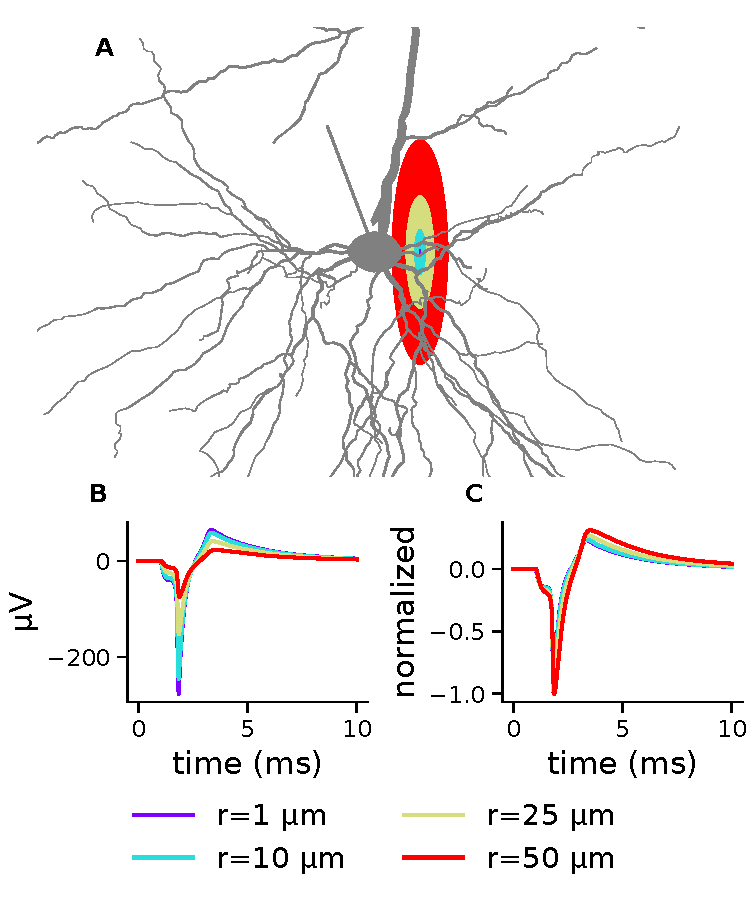
\includegraphics[width=0.6\textwidth]{Figures/Spikes/Spikes-fig_elec_size_effect.pdf}
\end{center}
\caption[]{\textbf{Effect of electrode size.}Bigger recording electrodes can cause smaller and broader EAPs.  \ghnote{Flott. Kursivere $r$? Forklare simuleringen?}
\gen{Veldig fin figur, som kanskje kan passe enda bedre here enn i VC-kapitlet "spikes" kapitlet. Hva tenker dere?}}
\label{fig:Spikes:electrode_size}
\end{figure}
%%%

The insulating electrode shaft effectively act to shadow spikes from neurons placed on the 'non-contact' side of the electrode.
Detailed studies of this requires comprehensive numerical investigations by use of FEM modeling~\cite**{Mechler2011,Mechler2012,Buccino2019}.

\subsection{\blue{Microelectrode arrays (MEAs)}}

Spikes are not only recorded in living brains. In \emph{in vitro} recordings, small slices of excised brain tissue are
placed in suitably designed dishes where physiological properties of cells and networks can be probed in detail for hours.
In so-called \emph{microelectrode arrays (MEAs)}, the bottom of the device is covered by a grid of electrode
contacts which record electrical signals generated by the neurons above. The brain slice and the MEA are both
covered with a liquid, typically saline, to protect the cells from drying out and keep them alive for the duration of the experiment, see
\Fref{fig:Spikes:MEA-setup}.

%%%
\begin{figure}[!ht]
\begin{center}
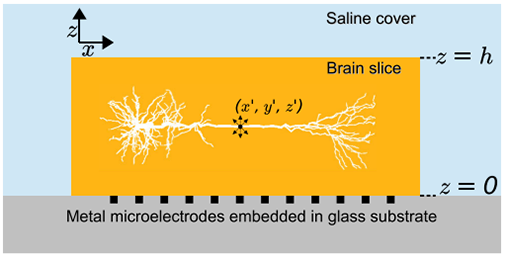
\includegraphics[width=0.7\textwidth]{Figures/Spikes/Spikes-MEA-1-w43-r300}
\end{center}
\caption[]{\textbf{MEA-setup.}
Figure is adapted from \citeasnoun**{Ness2015}.}
\label{fig:Spikes:MEA-setup}
\end{figure}
%%%

In MEAs the electrode contacts are embedded in an insulating glass plate with very 
low electrical conductivity, while the covering liquid typically has a higher electrical conductivity 
than the brain slice it covers. Thus the extracellular conductivity around the signal-generating neurons
will not be constant as assumed above, and this will affect the amplitude and shape of the recorded 
spikes. 

In general, FEM modeling will be required to solve the forward-modeling for situations such as this where
the the conductivity $\sigma$ varies with position. However, if we assume that the MEA substrate, slice and saline
all extend infinitely in the lateral directions so that $\sigma$ can be assumed to only have planar step-wise discontinuities, 
formulas analogous to \Fref{eq:XX:Vr} can be derived by use of the
\emph{method of images} from electrostatics. \gen{Referer til section i VC.}


%%%
\begin{figure}[!ht]
\begin{center}
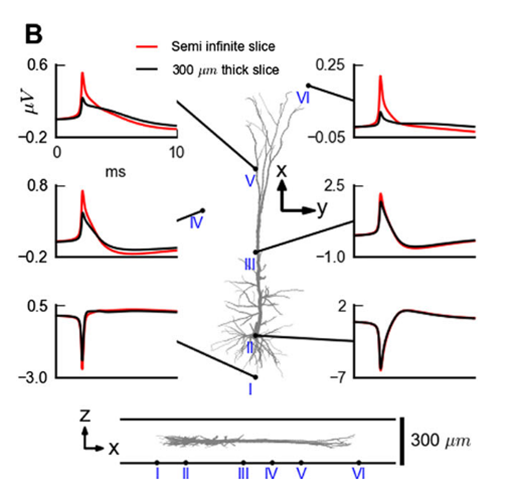
\includegraphics[width=0.8\textwidth]{Figures/Spikes/Spikes-MEA-2-w43-r300}
\end{center}
\caption[]{\textbf{MEA-spikes.}
Figure is adapted from \citeasnoun**{Ness2015}.}
\label{fig:Spikes:MEA-spikes}
\end{figure}
%%%

An example result is shown in \Fref{fig:Spikes:MEA-spikes}.
The largest effect on the spike comes from the insulating glass substrate which roughly doubles the size of the 
recorded spikes. However, also the highly-conductive 
saline cover employed in the example has an effect. More specifically, it
reduces the size of the spike compared to the hypothetical 
situation where the saline had the same value of the electrical conductivity as the brain slice.


\section{\blue{Multi-unit activity (MUA)}}

In general, a recording contact will pick up spikes from several neurons positioned in its vicinity, that is, from `multiple units'.
The term \emph{multi-unit activity (MUA)} refers to this total spiking activity seen in the high-frequency part of recorded extracellular potentials. 

%%%
\begin{figure}[!ht]
\begin{center}
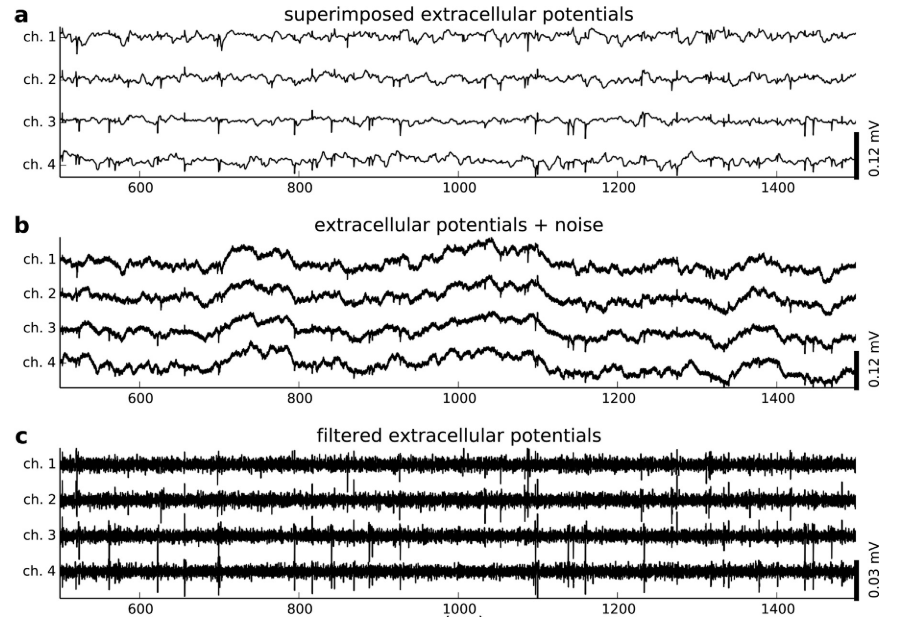
\includegraphics[width=0.8\textwidth]{Figures/Spikes/MUA-11}
\end{center}
\caption[]{\textbf{MUA tetrode}
Fra Hagen (2015):
Example benchmarking data for in vivo tetrode recordings. (a) Extracellular potential generated by population of six cortical pyramidal neurons.  
(b) Raw benchmarking data found from superposition of population potentials (from panel a) and synthesized model noise. (c) Filtered benchmarking data (corresponding to signals in (b)) showing MUA". 
Adapted from \citeasnoun**{Hagen2015}.
}
\gen{Kan vi kan legge til et panel som illustrerer en tetrode?}
\label{fig:Spikes:MUA-tetrode}
\end{figure}
%%%


\subsection{\blue{Spike extraction and sorting}}  

With only a single recording contact, the most direct way to analyse the MUA is to simply detect and count the spikes in the recorded 
signal trace. Here a suitable detection procedure must be used. This typically involves thresholding where only putative spikes larger than a 
preset threshold depending on the ambient noise level, are included. 
\gen{Kanskje vi kunne laget en enkel figur her?}

Today, spikes are typically recorded with multielectrodes, for example, 
tetrodes with four closely positioned recording contacts (\Fref{fig:Spikes:MUA-tetrode}), 
linear multielectrodes (polytrodes) with tens of contacts positioned along a straight line (\Fref{fig:Spikes:MUA-polytrode}), or 
grid-like multielectrodes with many hundred tiny contacts arranged in rectangular patterns on an electrode shaft \cite**{Jun2017}.  
On these multielectrodes, the same spike will in general show up on several contacts, and a process known as 
\emph{spike sorting}~\cite**{Quiroga2007} is required to (i) properly count spikes and (ii) to sort recorded spikes 
into contributions from individual neurons as is often the goal. 

To develop and validate methods for spike sorting, benchmarking data where the `ground truth' is known is highly desirable. Experimental benchmarking
data is hard to come by as they require simultaneous recording of intracellular action potentials and corresponding extracellular spikes.
However, model-based benchmarking data is an attractive alternative~\cite**{Einevoll2012} and the generation of such data has been pursued in several projects
\cite**{CamunasMesa2013,Hagen2015,MondragonGonzalez2017,Buccino2020}. 

An example is given in \Fref{fig:Spikes:MUA-tetrode} where virtual MUA signals
recorded by a tetrode is shown \cite**{Hagen2015}. The MUA signals have been computed by simulating six cortical neurons placed around a tetrode which are driven to spiking by a combination
of excitatory and inhibitory synaptic inputs (panel a). Further, noise with the same statistical properties as what is seen in real tetrode experiments, is added to the signal (panel b) 
prior to the high-pass filtering which results in the MUA benchmarking data (panel c). The final MUA data clearly shows how an action potential from a single neuron is seen
simultaneously as spikes on several of the tetrode contacts. 

Another example is given in \Fref{fig:Spikes:MUA-polytrode} where spikes from 16 cortical neurons are recorded by a 16-contact linear multielectode spanning the cortex. Here we observe that an action potential from a single neuron typically are observed as spikes at two to four adjacent contacts.



%%%
\begin{figure}[!ht]
\begin{center}
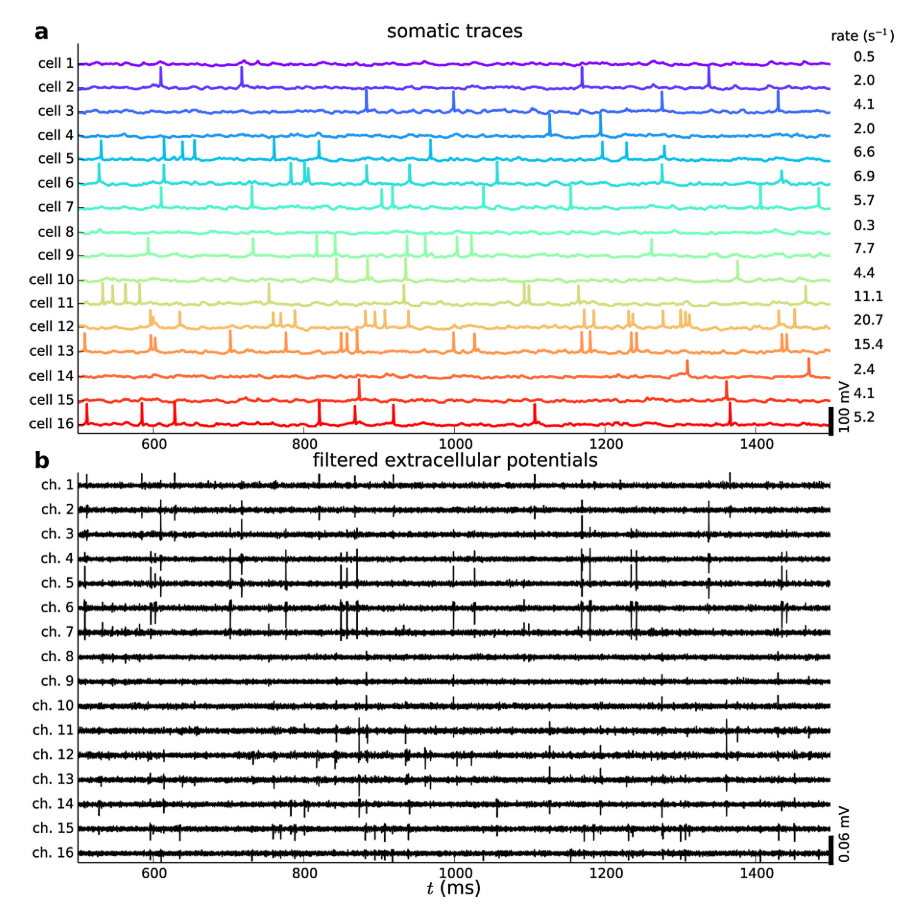
\includegraphics[width=0.8\textwidth]{Figures/Spikes/MUA-10}
\end{center}
\caption[]{\textbf{MUA linear multielectrode (polytrode)}
Fra Hagen 2015: Excerpts of intracellular and extracellular recordings for the 16 cells included in the example 16-channel polytrode benchmarking data set. 
(a) Somatic membrane potentials. Firing rates of cells 1-16 averaged over the 120 s real-time duration of the simulation are listed on the right hand side. (b) Superposition of extracellular potentials from all neurons and model noise, after band-pass filtering."
}
\gen{Kan vi kan legge til et panel som illustrerer polytroden?}
\label{fig:Spikes:MUA-polytrode}
\end{figure}
%%%

\subsection{\blue{Population firing-rate estimation from MUA}}  

The number of spikes that can be picked up above the ambient noise level by an electrode contact, depends on several factors. One is the volume density and morphological shapes of active
neurons around the contact. Another is the impedance and size of the contact itself. 
As discussed in \Fref{sec:Spikes:electrode_size} large electrode contacts will tend to reduce the spike amplitude through a spatial averaging effect, making it difficult to 
identify individual spikes from the recorded signal. If so, an estimate of the combined firing rate of the neurons surrounding the contact may be found by using the MUA signal in a different way,  that is, by rectification of the high-pass filtered extracellular potential~\cite**{Schroeder1998,Schroeder2001,Ulbert2001}. The principle behind this approach is illustrated
in \Fref{fig:Spikes:MUA-rectifify}.

%%%
\begin{figure}[!ht]
\begin{center}
%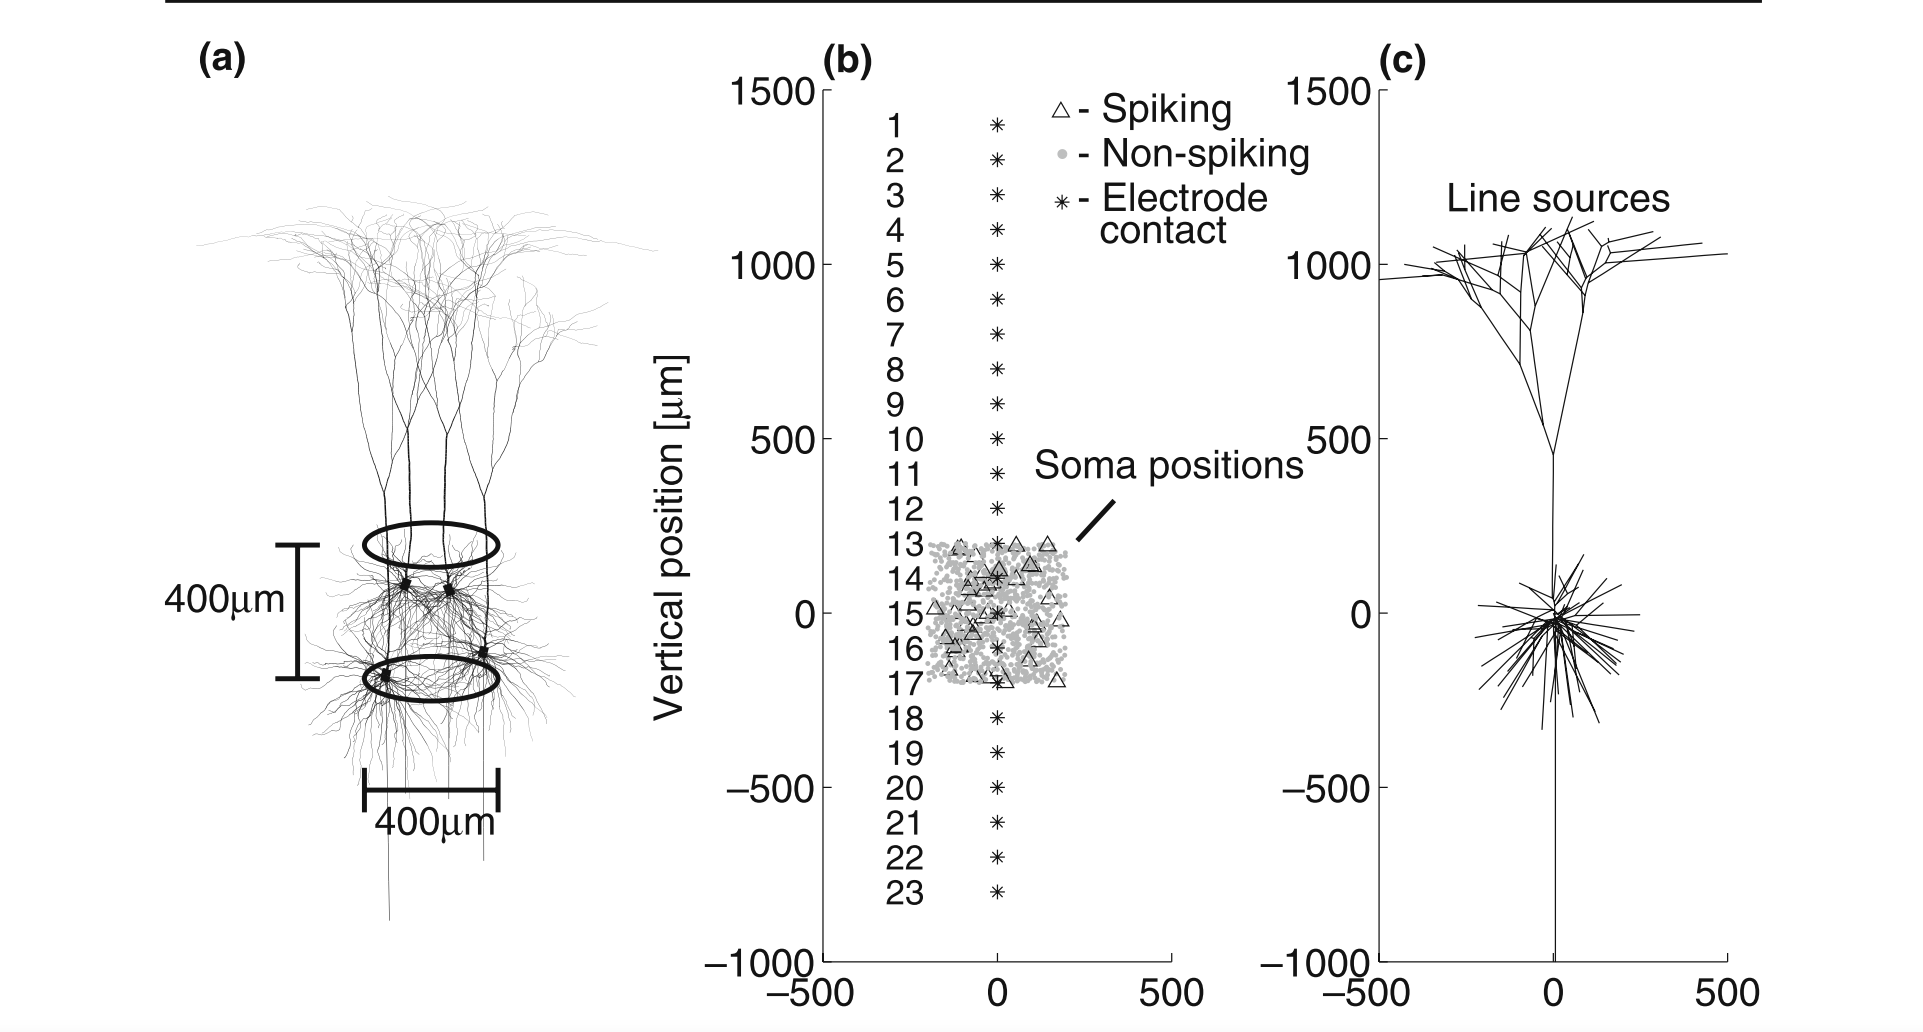
\includegraphics[width=0.8\textwidth]{Figures/Spikes/MUA-2}
\end{center}
\caption[]{
\gen{Figure illustrating principle behind MUA from rectification method}
\gen{Can you make such a figure, Torbj{\o}rn?}
}
\label{fig:Spikes:MUA-rectifify}
\end{figure}
%%%

The approach was used to estimate firing rates of cortical populations of neuron in the rat barrel (somatosensory) cortex based on multielectrode laminar 
recordings~\cite**{Einevoll2007,Blomquist2009}. To test the validity of the method, a modeling study was pursued where an analogous virtual (in silico) experiment 
was performed~\cite**{Pettersen2008}. Specifically, about thousand layer-5 cortical pyramidal neurons with somas arranged in a cylindrical disc, 
mimicking a neuronal population in rat barrel cortex, was considered (\Fref{fig:Spikes:MUA-population}). The neurons received synaptic inputs simulating a volley of synaptic activation following 
sensory stimulation from flicking the appropriate whiskers. Extracellular potentials were computed for a set of contact positions along the central axis of the cylinder (\Fref{fig:Spikes:MUA-population}B).

%%%
\begin{figure}[!ht]
\begin{center}
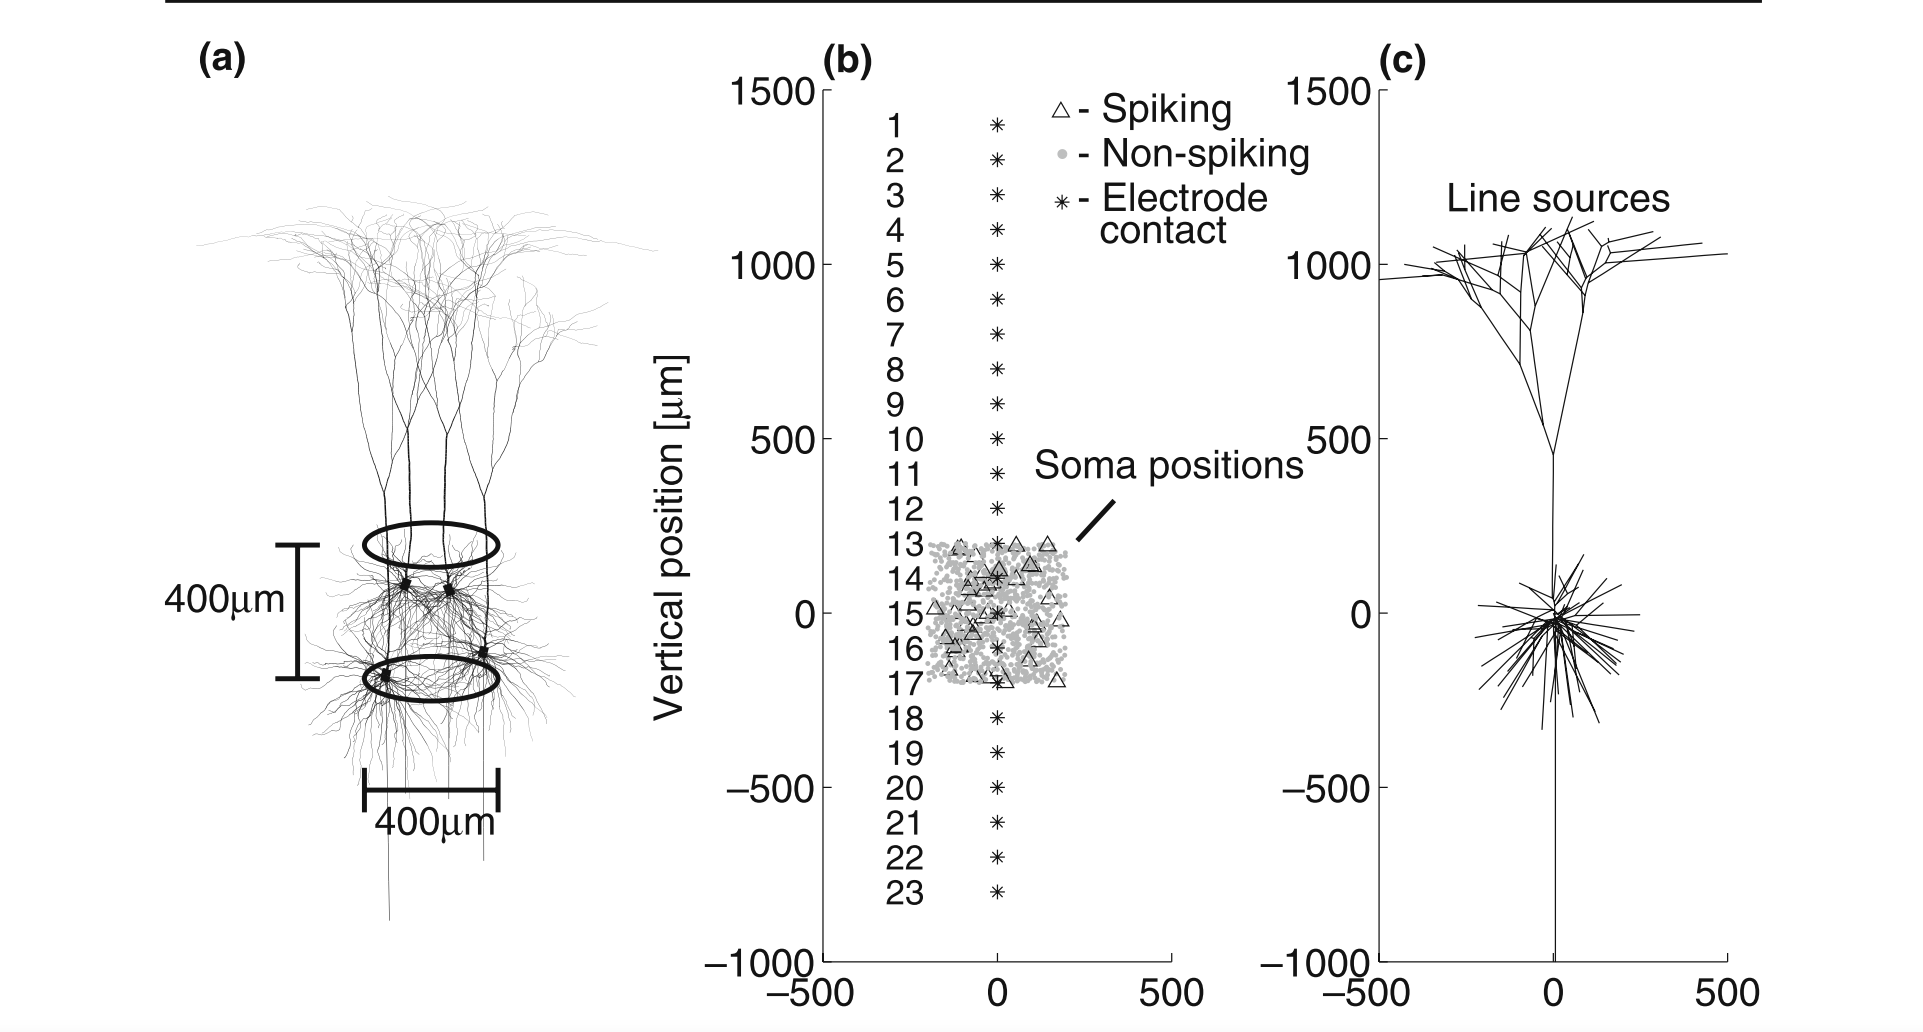
\includegraphics[width=0.8\textwidth]{Figures/Spikes/MUA-2}
\end{center}
\caption[]{
From Pettersen 2008a: \textbf{Schematic illustration of neural population created from pyramidal layer-5 neuron templates.} (b) Somas of neuronal templates are placed randomly inside a cylindrical annulus with height h=0.4 mm, outer diameter d=0.4 mm, and inner diameter 0.1 mm. One thousand cells are non-spiking (dots), while 40 cells produce a single spike following synaptic stimulation
(triangles). The electrode point contacts (stars) are aligned on the central axis of the cylindrical annulus. (c) Illustration of line-source method where the transmembrane currents passing through the 
segments of the displayed branches are modeled as line segments with uniform current density.}
\label{fig:Spikes:MUA-population}
\end{figure}
%%%

An example result is shown in \Fref{fig:Spikes:MUA-ApicalSynapses}. Here panel A shows the total extracellular potential following the synaptic activation of the population. The signal
is dominated by the low-frequency response to the synaptic input, that is, the local-field potential (LFP). The spatial pattern of the signal across recording channels reflects the
spatial distribution of synaptic inputs onto the pyramidal neurons. In this example, excitatory synapses are placed on the apical dendrites while inhibitory synapses are placed on the basal dendrites.
The dominance of low frequencies in the signal is illustrated in panel B showing the Fourier transformed signal, that is, the amplitude of each frequency component, for three of the channels.
Here it can be seen that the frequencies up to 100 Hz dominate the signal completely, that is, have the highest amplitudes (and power, corresponding to the amplitude squared). 

%%%
\begin{figure}[!ht]
\begin{center}
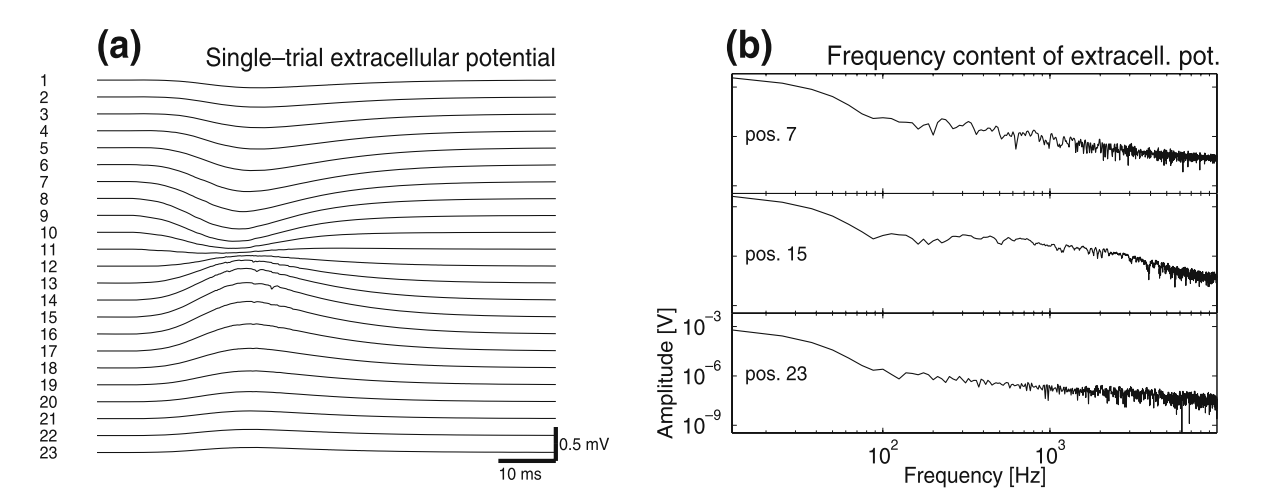
\includegraphics[width=0.8\textwidth]{Figures/Spikes/MUA-3} \\
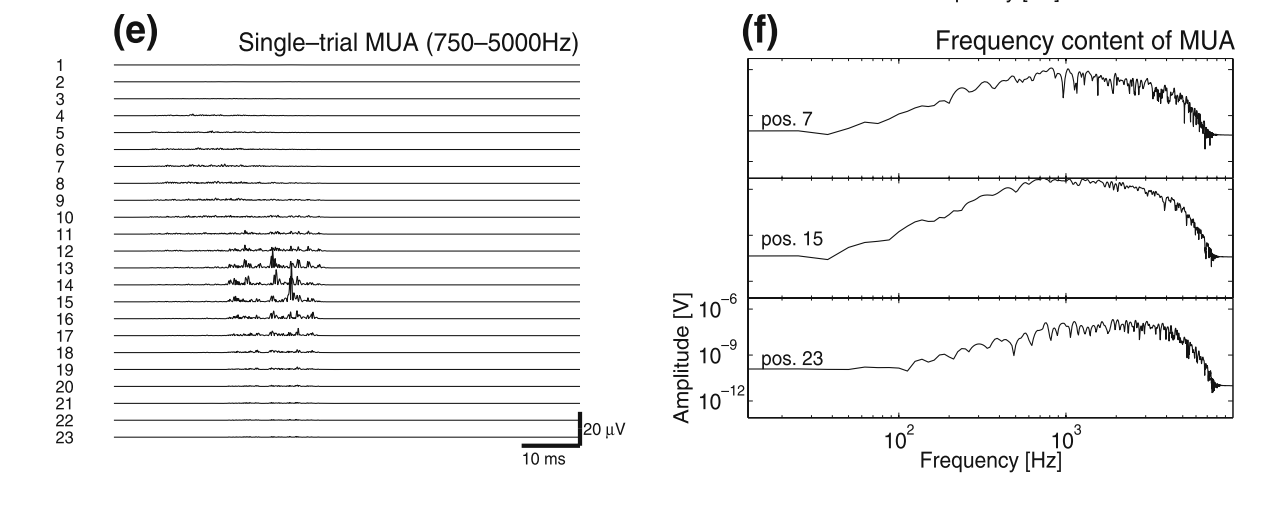
\includegraphics[width=0.8\textwidth]{Figures/Spikes/MUA-4} \\
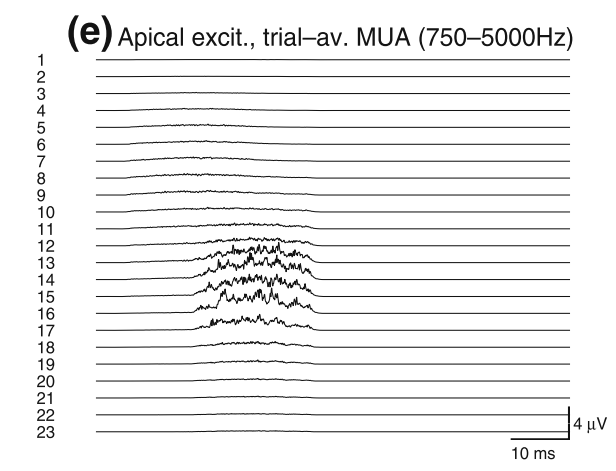
\includegraphics[width=0.4\textwidth]{Figures/Spikes/MUA-5} 
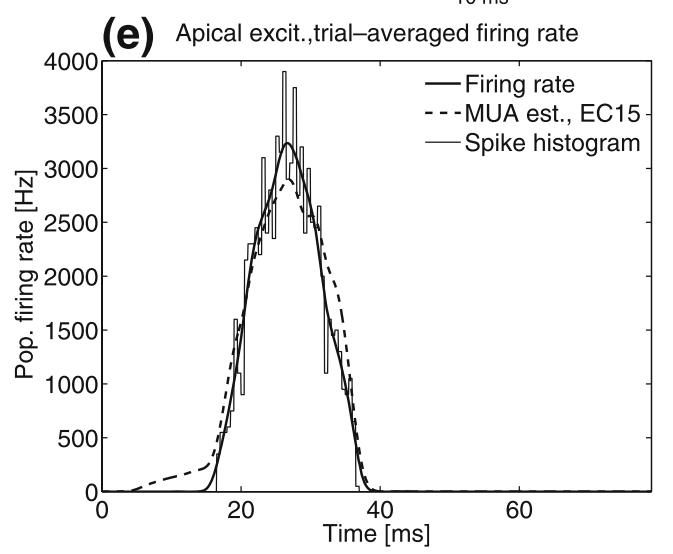
\includegraphics[width=0.4\textwidth]{Figures/Spikes/MUA-7} 
\end{center}
\caption[]{
From Pettersen 2008a: \textbf{Extracellular potentials at electrode contacts 1-- 23 for apically stimulated population.} 
(a) Single-trial raw (unfiltered) extracellular potentials. 
(b) Frequency content, i.e., Fourier amplitudes, of raw potentials in (a). 
Middle left: "(e)" MUA, i.e., high-pass filtered (750 -- 5.000 Hz) and rectified content of potentials in (a). 
Middle right "(f)" Frequency content of the MUA in (e) prior to rectification. The mean synaptic onset times are stochastically distributed around 20 ms with a standard deviation of $\sigma$=5 ms.
Lower left: "(e)": MUA, i.e., high-pass filtered (750 -- 5.000 Hz), rectified and then trial-averaged signals for apically excited population. 
Lower right: "(e)": Spike histogram (bin width 0.5 ms), `true' population firing rate, and estimated firing rate from the MUA of electrode contact 15. The amplitude of the estimated firing rate
has been fitted to minimize the relative mean square deviation er  between the estimated and `true' population firing rates. 
\gen{Refer to Pettersen2008 for detailed explanation.}
}
\label{fig:Spikes:MUA-ApicalSynapses}
\end{figure}
%%%

While the spikes are buried by the low-frequency components in the raw signal, they can be extracted by high-pass filtering 
and subsequent rectification. Results are shown in \Fref{fig:Spikes:MUA-ApicalSynapses}, as a function of time in panel C
and in frequency space in panel D. \gen{Panel labeling is wrong in present figures}
A first observation in panel C is
that the remaining signal is confined to channels deep in the cortex, that is, close to the somas of the neurons in the populations.
This reflects that extracellular signatures of action potentials are typically confined to within 100~$\mu$m from the soma, cf. \Fref{fig:Spikes:DifferentNeuronModels}. A second observation in panel C is that the MUA signals 
only last for about 20~ms, which turns out to be the time period in which the neurons in the model fire action potentials~\cite**{Pettersen2008}.
A third observation is that the MUA signal is not smooth, but `noisy' in the sense that it
consists of a collections of sharp peaks of different heights. This `noisiness' stems from the inherent randomness both in the times of spiking 
and the positions of the somas of the low number (40) of spiking neurons in the population. 

In sensory systems it has been common to measure 
trial-averaged responses, that is, the response averaged over many repetitions of the same stimulus. The rationale is that this procedure highlights the contributions from sensory input in that the effects of other synaptic inputs and noise in sensory neurons are reduced. The trial-averaged MUA found from averaging MUA results from forty model trials, is shown in 
panel E of \Fref{fig:Spikes:MUA-population}, revealing a much less `noisy' signal. 

The obvious next question is to what extent the resulting MUA signal gives a good measure of the population firing rate. Unlike in experiments, the true underlying firing rate is known in the model, allowing for a quantitative comparison. The question was studied in detail for the model in question in \citeasnoun**{Pettersen2008}. The noisyness of MUA signals from individual trials (\Fref{fig:Spikes:MUA-population}C) did not allow for accurate estimation of firing rates in individual trials. However, accurate estimates for trial-averaged firing rates (commonly referred to as Post Stimulus Time Historgrams (PSTHs)) could be obtained from trial-averaged MUA signals. 
An example is given in \Fref{fig:Spikes:MUA-ApicalSynapses}F. Here a firing-rate estimate based on the MUA signal from one of the recording channels positioned at a depth in the midst of somas of the population is compared with the true, temporally smoothed firing rate.  
The overall agreement is observed to be quite good.

 One deviation is that the MUA signal predicts a non-zero firing rate prior to the onset of true firing, the reason being that the synaptic input current itself gives a contribution to the MUA signal. Another deviation is that the MUA-based firing rate predicts a too low maximum firing rate, due to cancellations of signal contributions from temporally overlapping spikes from different neurons. This latter effect increases with increasing firing rates and can be remedied by assuming a supralinear relationship between the MUA signal and firing rate \cite**{Pettersen2008}.  The accuracy of the population firing rate can also be improved by using MUA signals from several adjacent recording channels in the estimation \cite**{Pettersen2008}.  
 
The accuracy of this MUA-based estimation of population firing rates will depend on the specific situation considered. In \citeasnoun**{Pettersen2008}, it was, for example, found
that the prediction was slightly more accurate when the population in \Fref{fig:Spikes:MUA-population} is driven by excitatory inputs onto the basal dendrites rather than onto the
apical dendrites as in \Fref{fig:Spikes:MUA-ApicalSynapses}.
 
%
%%%%
%\begin{figure}[!ht]
%\begin{center}
%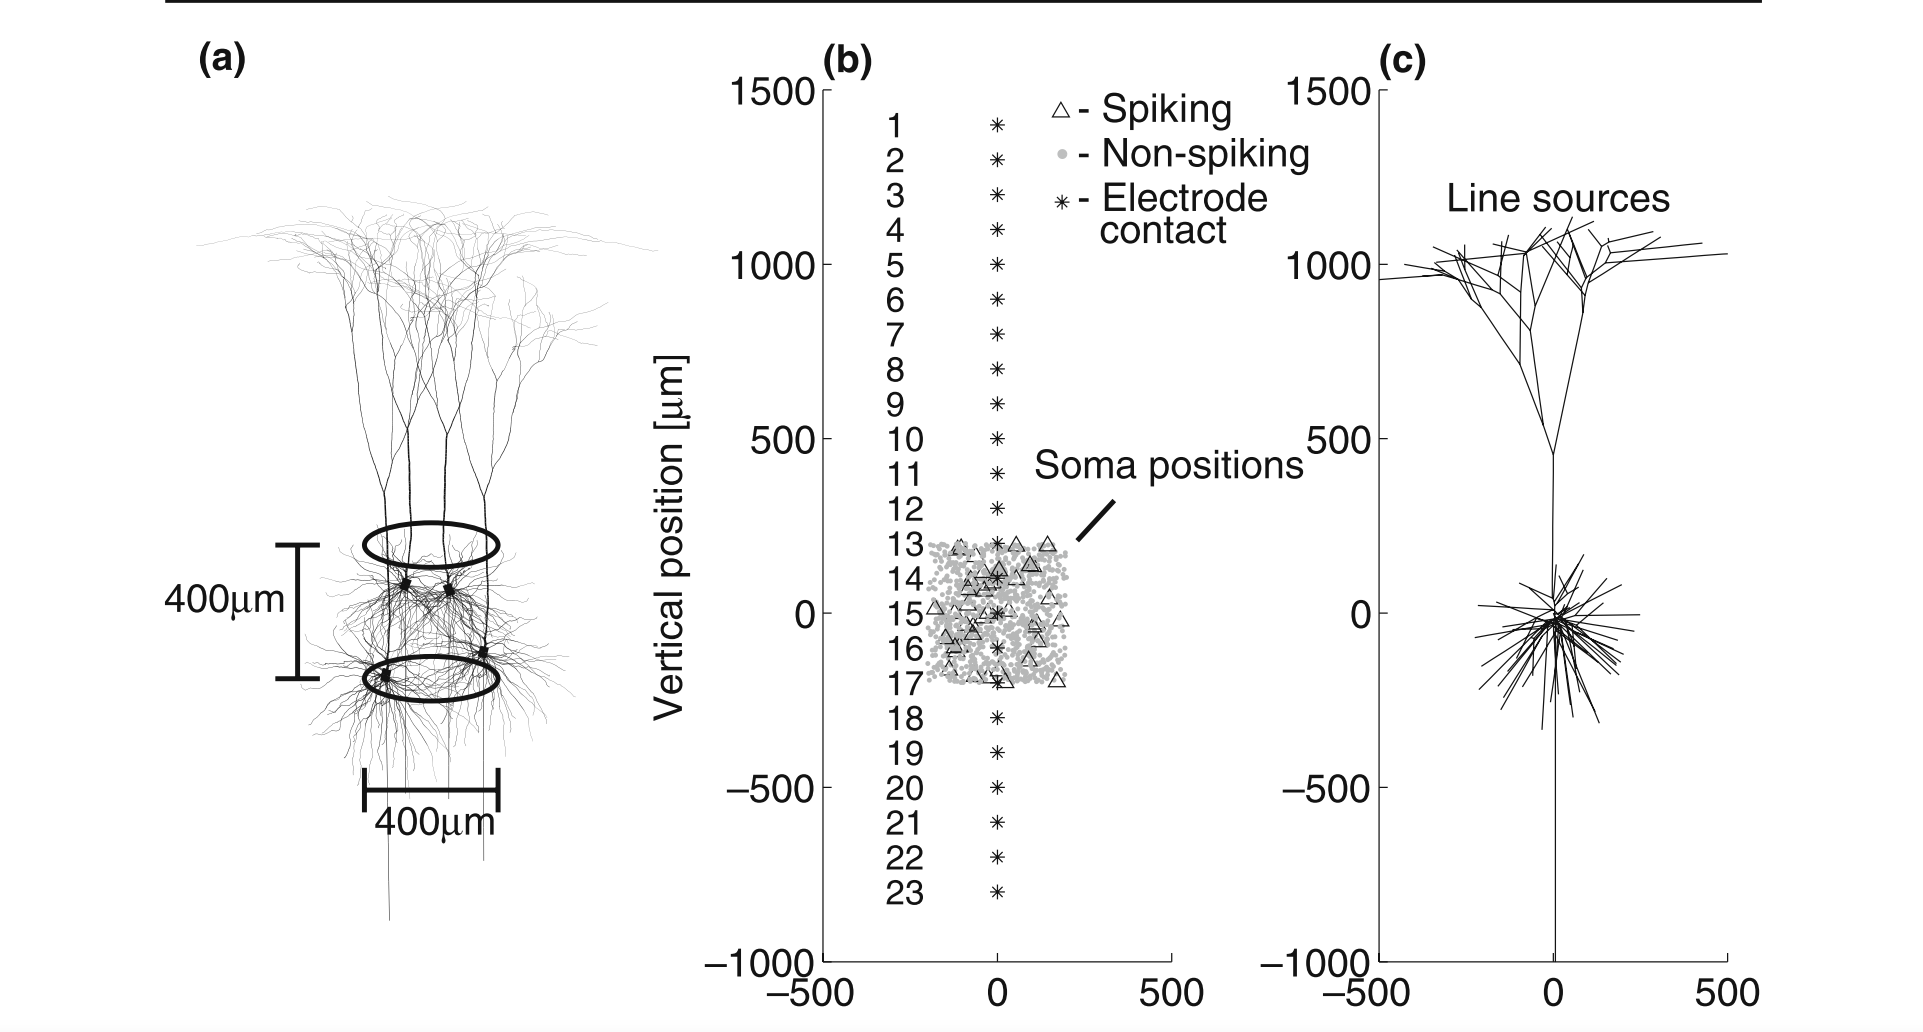
\includegraphics[width=0.8\textwidth]{Figures/Spikes/MUA-2}
%\end{center}
%\caption[]{\textbf{MUA}}
%\label{fig:Spikes:MUA-A}
%\end{figure}
%%%%
%

%
%%%%
%\begin{figure}[!ht]
%\begin{center}
%\includegraphics[width=0.4\textwidth]{Figures/Spikes/MUA-6}\\
%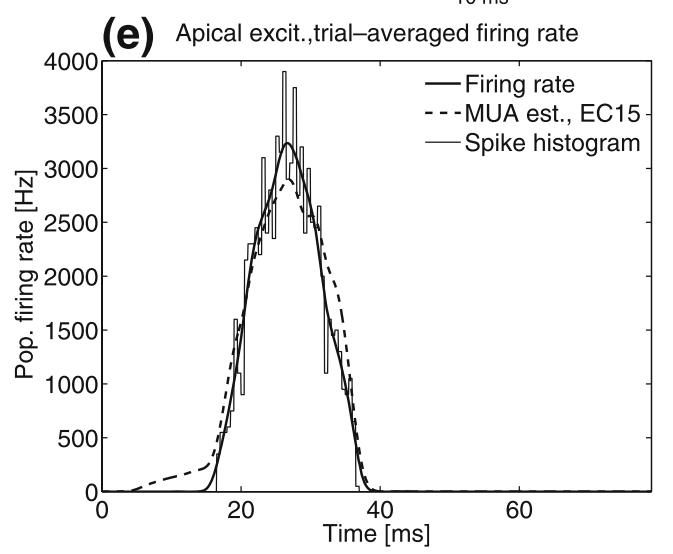
\includegraphics[width=0.4\textwidth]{Figures/Spikes/MUA-7}
%\end{center}
%\caption[]{\textbf{MUA}}
%\label{fig:Spikes:MUA-C}
%\end{figure}
%%%%
%
%%%%
%\begin{figure}[!ht]
%\begin{center}
%\includegraphics[width=0.8\textwidth]{Figures/Spikes/MUA-8}
%\end{center}
%\caption[]{\textbf{MUA}}
%\label{fig:Spikes:MUA-D}
%\end{figure}
%%%%
%

%\section{\red{Insights from MUA studies}} 
%\ghnote{I added this kind of subsection to most of the Part 2 - sections. I thought it might be an idea to finish the MUA, LFP, ECoG and EEG sections with summaries of what these modalities typically tell us, i.e. in terms of (i) what aspects of neural activity they reflect (spikes, synaptic inputs, dendritic ion channels, which ion channels, which kind of neurons, something on network structure, cell orientation, cortical folding etc.), and what what they can tell us about cognitive states (attentive, drowsy etc.). I am not sure about this idea, though. Maybe it will be too challenging to get an overview over the literature - we dont want to put the entire Nunez-book into the EEG-chapter.}

%%%%%%%%%%%
%% Box: Spike sorting
%%%%%%%%%%%
%%\begin{boxfloat}{Spike sorting}
%%  \label{mm:box:spike-sorting}
%\subsection{\red{Box: Spike-sorting}}
%\gen{This was a Box in the Sterratt chapter}
%%
%\centerline{\includegraphics{Figures/Spikes/Spikes-sorting-w35-r300}}\vspace*{6pt}
%%
%A sharp electrode placed in brain tissue will pick up spiking signals from several neurons. 
%However, the shapes of the spikes will be different for the different neurons, and this can be used to sort the spikes according to their neurons of origin. This is referred to as \index{spike sorting}, 
%and is a problem of great practical importance both for neuroscience research and development of neuroprosthetic devices. 
%
%In the present day with electrodes with hundreds or thousands of electrode recording contacts, fast and accurate automatic spike-sporting methods are needed to replace time-consuming manual spike-sorting methods~\cite**{Quiroga2007}. To develop and test such automatic methods, one needs
%benchmarking spiking data where the `ground truth', that is, the actual spiking times for the contributing neurons, is known~\cite**{Einevoll2012}.
%One use of the EP modelling scheme for spikes has been to generate such benchmarking data~\cite**{CamunasMesa2013,Hagen2015,MondragonGonzalez2017}. 
%
%Modern electrodes have numerous recording contacts, often placed only some micrometers apart. Thus a spike can be measured at several contacts
%simultaneously, each contact recording a slightly different shape reflecting the different positions of the contacts relative to the spiking neuron. 
%This not only allows for accurate spike sorting, but also for estimation of the spatial position of the neuron. Likewise, the spatial variation of the 
%spike shape around the neuronal soma (see Figure~\Fref{fig:Spikes:MultiCompartment}) 
%depends on the details of the intracellular action potential and dendritic morphology thus also allowing for the 
%identification of neuron type~\cite**{Buccino2018}.    
%\gen{Figure to be adapted from Quiroga (2007).}
%%\end{boxfloat}
%%%%



%While the formulae above were derived for a neuron model with a single passive dendritic stick, similar expressions can be derived for 
%more complicated neuron models where several passive sticks protrude from the soma, see \citeasnoun**{Pettersen2008}.
%The main conclusions above hold also for these neuron models, in particular that spike widths always increase with distance and that
%the amplitude of a spike is proportional to $d^{k}$ where $k\sim1.5-2$. For neurons with many dendrites attached to the 
%soma, the contributions to the spike amplitude roughly adds up. A simple rule of thumb is that a neuron's spike amplitude is 
%roughly proportional to the sum of the cross-sectional areas for all dendrite branches attached directly onto to the soma. Neurons with many thick
%dendritic branches attached to the soma will thus generate the largest spikes. See~\citeasnoun**{Pettersen2008} for further discussion.
%
%
%{\bf TEXT COPIED FROM STERRATT CHAPTER ON 2020-10-13}
%
%\section{Dependence of spike size and shape on neuronal properties}
%
%Extracellular measurement of spikes from a neuron in living brains is blind in the sense that it is
%not known what type of neuron is recorded from when an electrode is lowered into the brain.
%Some neuron types produce spikes with larger amplitudes and/or broader shapes than
%others,
%%
%%\todo{TVN: Nevne at det ofte sorteres i "putative excitatory" og "putative inhibitory"?}
%%
%and as seen in Figure~\Fref{mm:fig:EP-spike-MultiCompartment} both the shape and amplitude 
%depend critically on recording positions. Large spike amplitudes imply that they will be more dominant in electrical recordings,
%and ideally this bias should  be considered in the analysis of joint recordings 
%of spikes from many neurons. 
%
%To understand the link between the morphology of neurons and their spike amplitudes and shapes
%it is convenient to consider ball-and-stick neurons where a passive dendrite cable `stick' is connected to a point-like soma.
%Despite its simplicity, the ball-and-stick neuron model exhibits the key qualitative features observed in
%Figure~\Fref{mm:fig:EP-spike-MultiCompartment} when the multi-compartmental EP formula in 
%\Fref{mm:equation:Ve-multi-compartment}
%is used; that is, rapid attenuation of spike amplitude and increased spike width as the distance from the soma 
%increases \cite**{Pettersen2008,Pettersen2012}. 
%
%\citeasnoun**{Pettersen2008} took advantage of the mathematical tractability of the ball-and-stick model to
%derive analytical expressions for how the amplitude of the recorded spike depends on distance from the neuron as well
%as the electric properties of the neuron. The action potentials were decomposed into contributions from
%many frequency components and each frequency component was considered individually.
%This is illustrated in Figure~\Fref{mm:fig:EP-spike-ball-and-stick-frequency} where the amplitudes of the different frequency components needed to
%represent the intracellular action potential (membrane potential) and extracellular spike respectively are shown.
%A key observation here is that for the extracellular spike, the largest contributions comes from frequencies larger than 100~hertz.
%%%%%%%%%%%
%% Figure: Action potential and its frequency content
%%%%%%%%%%%
%%\begin{cnfigure}{Figures/fig-not-pushed-to-github}
%%\begin{cnfigure}{Figures/mm/EP-spike-ball-and-stick-frequency-w90-r150}
%%\caption[]{
%%Frequency content of example intracellular (a) and extracellular spike (b).
%%%
%%%(a) Action potential used in simulations in Figure~\Fref{mm:fig:EP-spike-ball-and-stick-results}(inset) 
%%%\todo{Comment from DCS not understood.}
%%%and its frequency content. 
%%%%The intracellular spike width is defined as the
%%%%width of the AP at half amplitude and is 0.55~ms for the standard
%%%%AP, and half the value for the narrow AP. 
%%%(b) Frequency content of example extracellular spike.
%%%Inset: Typical spike shape computed a distance $r=10~\mu$m
%%%perpendicular to the dendrite at the level of soma for a ball-and-stick 
%%%neuron with diameter $d=2~\mu$m and infinite dendrite length.
%%%Here the intracellular action potential in left panel was imposed as a voltage-clamp in the soma.
%%%The extracellular spike width is defined as the width of the negative phase at 25\% of its maximum
%%%amplitude and is 0.44~ms for the example spike.
%%%The amplitude (peak-to-peak value) of the spike is $56~\mu$V  
%%\todo{Figure + caption to be updated. Will only include standard AP in final figure.} 
%%Adapted from \citeasnoun**{Pettersen2008}.
%%}
%%\label{mm:fig:EP-spike-ball-and-stick-frequency}
%%\figpermOurs
%%\end{cnfigure}
%
%
%%\todo{Explain the idea that the question is about how currents entering the soma during the AP returns through the dendrite}
%
%\citeasnoun**{Pettersen2008} derived simple formulae relating the intracellular action potential to the extracellular spike for two limiting cases:
%when the recording is done near to the soma or far away from the soma. For recordings near the soma the 
%amplitude $|\hat{V}_\mathrm{e,near}(f,\vec{r})|$ of the spike signal for each frequency component with frequency $f$ was found to be approximated
%by
%%
%\begin{equation}
%  |\hat{V}_\mathrm{e,near}(f,\vec{r})| 
%  \propto \frac{d^{3/2}}{r} \sqrt{ \frac{f C_\mathrm{m}}{R_\mathrm{a}} }  |\hat{V}_\mathrm{s}(f)| 
%  \label{mm:equation:Ve_near}
%\end{equation}
%%
%Here $|\hat{V}_\mathrm{s}(f)|$ is the amplitude of frequency component of the soma membrane potential at the same
%frequency (see Figure~\Fref{mm:fig:EP-spike-ball-and-stick-frequency}).
%For recording positions far away from the soma, the following expression was instead found:
%%%%
%\begin{equation}
%  |\hat{V}_\mathrm{e,far}(f,\vec{r})|  \propto d^{2} \frac{|\cos \theta| }{r^2  R_\mathrm{a}}  |\hat{V}_\mathrm{s}(f)| 
%  \label{mm:equation:Ve_far}
%\end{equation}
%%%%
%In these formulas, $d$ is the diameter of the dendritic
%stick, $C_\mathrm{m}$ the specific membrane capacitance, and $R_\mathrm{a}$ the specific axial resistance.  
%

%%%%%%%%%%%
%% Figure: Spike widths and amplitudes
%%%%%%%%%%%
%\begin{cnfigure}{Figures/mm/EP-spike-ball-and-stick-results-w100-r150}
%\caption[]{
%Spike widths (left) and (peak-to-peak) spike amplitudes (right) as a function of
%distance from soma for a detailed pyramidal cell model (pyramidal) and two
%types of ball-and-stick models: long, finite ball-and-stick
%model (fin.~stick, long) with diameter $d=2~\mu$m and length
%$l=1$~mm and a short, finite ball-and-stick model (fin.~stick, short) with diameter $d=1~\mu$m and length $l=0.2$~mm,
%see Figure~\Fref{mm:fig:EP-spike-ball-and-stick-neuron-models}.
%The intracellular action potential shown in the inset in the left panel of 
%Figure~\Fref{mm:fig:EP-spike-ball-and-stick-frequency} was imposed as a voltage-clamp in the soma.
%The EP was recorded in the
%somatic plane normal to the stick/primary apical dendrite. 
%In right panels guidelines illustrating the power-law decays $1/r$ and
%$1/r^{2}$ have been added. 
%For further details see \citeasnoun[Figure 6]{Pettersen2008}.
%\todo{Figure + caption to be updated. Adapted from \citeasnoun**{Pettersen2008}.}
%}
%\label{mm:fig:EP-spike-ball-and-stick-results}
%\figpermOurs
%\end{cnfigure}


%\paragraph{Spike amplitude dependence on distance}

%%%%%%%%%%%%%%%%%%%%%%%%%%%
%% Box: Spike sharpness
%%%%%%%%%%%    
%\begin{boxfloat}{Spike sharpness}
%  \label{mm:box:spike-sharpness}
%There are several qualitative insights regarding the sizes and widths of spikes that can 
%be found from the near-field and far-field formulae in Equations~\Fref{mm:equation:Ve_near} and 
%\Fref{mm:equation:Ve_far}, respectively. One relates directly to the shape of the spike:
%in the near-field expression, the high-frequency components of the spike is amplified 
%compared to the low-frequency components, that is, $\hat{V}_\mathrm{e,near}(f,r) \propto \sqrt{f}$.
%Thus close to the soma the spike is observed to be sharper than the intracellular action potential
%as observed in the insets in Figure~\Fref{mm:fig:EP-spike-ball-and-stick-frequency}. 
%In the far-field regime there is no such high-frequency amplification ($\hat{V}_\mathrm{e,near}(f,r) \propto f^0 \sim 1$).
%As a consequence, spikes measured far away from the soma will have less high-frequency content than those measured close to soma.
%Thus the far-away spikes will be blunter and have larger spike widths as seen in the spike-width panel of 
%Figure~\Fref{mm:fig:EP-spike-ball-and-stick-results}.
%%
%%\centerline{\includegraphics{Figures/mm/MEA-1-w43-r300}}\vspace*{6pt}
%%
%\end{boxfloat}
%%%%%%%%%%%%%%%%%%%%%%%%%%%%%%%%





%
%%%%%%%%%%%
%% Sidebox: Fourier sum
%%%%%%%%%%%
%\begin{sidebox}
%Time signals, such as the time course of a spike $V_\mathrm{e}(t)$,  can conveniently 
%be represented as a sum of \firstterm{Fourier components} with different frequencies $f$. 
%Such a Fourier sum can be constructed in
%various ways. The derivations in 
%Section~\Fref{mm:sec:spike-widths-amplitudes}, building on \citeasnoun**{Pettersen2008}, use the  
%convention that a time signal $S(t)$ is the real part of the complex sum $\sum_{f}  \hat{S}(f) \exp (j 2 \pi f t)$. 
%Here $j$ is the unit of imaginary numbers, and  $\hat{S}(f)$ is in general a complex number. 
%\end{sidebox}
%%
%
%%%%%%%%%%%
%% Figure: Spike widths and amplitudes
%%%%%%%%%%%
%\begin{cnfigure}{Figures/mm/EP-spike-ball-and-stick-results-w100-r150}
%\caption[]{
%Spike widths (left) and (peak-to-peak) spike amplitudes (right) as a function of
%distance from soma for a detailed pyramidal cell model (pyramidal) and two
%types of ball-and-stick models: long, finite ball-and-stick
%model (fin.~stick, long) with diameter $d=2~\mu$m and length
%$l=1$~mm and a short, finite ball-and-stick model (fin.~stick, short) with diameter $d=1~\mu$m and length $l=0.2$~mm,
%see Figure~\Fref{mm:fig:EP-spike-ball-and-stick-neuron-models}.
%The intracellular action potential shown in the inset in the left panel of 
%Figure~\Fref{mm:fig:EP-spike-ball-and-stick-frequency} was imposed as a voltage-clamp in the soma.
%The EP was recorded in the
%somatic plane normal to the stick/primary apical dendrite. 
%In right panels guidelines illustrating the power-law decays $1/r$ and
%$1/r^{2}$ have been added. 
%For further details see \citeasnoun[Figure 6]{Pettersen2008}.
%\todo{Figure + caption to be updated. Adapted from \citeasnoun**{Pettersen2008}.}
%}
%\label{mm:fig:EP-spike-ball-and-stick-results}
%\figpermOurs
%\end{cnfigure}
%
%%%%%%%%%%%
%% Figure: Frequency-dependent distribution of return currents
%%%%%%%%%%%
%\begin{cnfigure}{Figures/mm/EP-spike-ball-and-stick-sketch-w70-r300}
%%\begin{cnfigure}{Figures/fig-not-pushed-to-github}
%\caption[]{Illustration of ball-and-stick neuron and its frequency-dependent 
%distribution of dendritic return currents following injection of a sinusoidal current into the soma.
%The net current entering the soma will enter the dendrite as an axial current, and return to the 
%ECS via the dendrite membrane. The inset shows the spatial distribution of this return current
%for different frequencies. The higher the frequency, the closer the return currents will be and
%the smaller the frequency-dependent length constant $\hat{\lambda}(f)$, reflecting the weighted mean 
%of the return-current positions (see sidebox), will be. 
%\todo{Figure + caption to be updated. Adapted from \citeasnoun**{Pettersen2012}.}
%\todo{June 2019: Move inbset to Ch. 5?}
%}
%\label{mm:fig:EP-spike-ball-and-stick-sketch}
%\figpermOurs
%\end{cnfigure}
%%
%
%
%
%%%%%%%%%%%
%% Box: Ball-and-stick model for spikes
%%%%%%%%%%%
%\begin{boxfloat}{Ball-and-stick model for spikes}
%  \label{mm:box:ball-and-stick-spikes}  
%To understand the dependence of spike shapes and amplitudes on model parameters for the ball-and-stick neuron, it is useful
%to consider the EP set up by each of the frequency (Fourier) components of the action potentials separately. 
%For recording positions $\vec{r}$ very close to the soma, the contribution from the soma current will dominate over the contributions from the dendrite 
%in the sum giving the EP in \Fref{mm:equation:Ve-multi-compartment}. Then the amplitude of the
%predicted oscillating EP $|\hat{V}_\mathrm{e,near}(f,\vec{r})|$ is approximately given by 
%%
%\begin{equation}
%  |\hat{V}_\mathrm{e,near}(f,\vec{r})| = \frac{|\hat{I}_\mathrm{s}(f)|}{4 \pi \sigma r} 
%  \label{mm:box:equation:Ve_near_1}
%\end{equation}
%%
%where $|\hat{I}_\mathrm{s}(f)|$ is the amplitude of the oscillating current through the soma membrane.
%%and also the axial current entering the dendrite from the soma compartment. 
%For the relatively high frequencies of most relevance for the spike, this soma current is related to the soma membrane potential 
%$\hat{V}_\mathrm{s}(f)$ through~\cite**{Pettersen2008}
%%
%\begin{equation}
%  |\hat{I}_\mathrm{s}(f)| =  \frac{\pi^{3/2} d^{3/2}}{\sqrt{2}} \sqrt{ \frac{f C_\mathrm{m}}{R_\mathrm{a}} }  |\hat{V}_\mathrm{s}(f)|
%  \label{mm:box:equation:Isoma}
%\end{equation}
%%
%and the spike EP is thus found to be
%%
%\begin{equation}
%  |\hat{V}_\mathrm{e,near}(f,\vec{r})| 
%  = \frac{\sqrt{\pi}}{4 \sqrt{2} \sigma}
%     \frac{d^{3/2}}{r} 
%     \sqrt{ \frac{f C_\mathrm{m}}{R_\mathrm{a}} }  |\hat{V}_\mathrm{s}(f)| 
%  \propto \frac{d^{3/2}}{r} \sqrt{ \frac{f C_\mathrm{m}}{R_\mathrm{a}} }  |\hat{V}_\mathrm{s}(f)| 
%  \label{mm:box:equation:Ve_near_2}
%\end{equation}
%%
%\todo{June 2019: Coordinated with or moved to Ch. 5.}
%%
%For recording positions further away from the soma, the contribution from return membrane currents must be taken into
%account in the sum in \Fref{mm:equation:Ve-multi-compartment}. An approximate way of doing this is to
%assume all return currents to leave the dendrite at a single height $\lambda_\mathrm{AC}(f)$ above the soma, where 
%this frequency-dependent length constant corresponds to the weighted mean of the positions of the return currents along
%the dendrite stick. (The subscript `AC' denotes `alternating current'.)
%Then the EP can be approximated by using the 
%dipolar expression in \Fref{mm:equation:Ve-dipole-p}, that is,
%%%%
%\begin{equation}
%  |\hat{V}_\mathrm{e,far}(f,\vec{r})| =  \frac{|p(f) \cos \theta|}{4 \pi \sigma r^2} 
%                                            = \frac{| \hat{I}_{s}(f) \lambda_\mathrm{AC}(f) \cos \theta|}{4 \pi \sigma r^2}   
%                                                                                        \label{mm:box:equation:Ve_far_1}
%\end{equation}
%%%%
%One way to define an AC length constant is as the mean value of the 
%envelope of the sinusoidally varying (normalized) membrane current
%$\hat{i}_\mathrm{m}$ weighted with distance $z$ from soma, 
%see Figure~\Fref{mm:fig:EP-spike-ball-and-stick-sketch}. 
%For an infinite dendrite stick this corresponds to
%%
%\begin{equation}
%  \lambda_\mathrm{AC}^\infty(f) = \frac{\int_0^\infty z |\hat{i}_\mathrm{m}| dz}{\int_0^\infty |\hat{i}_\mathrm{m}| dz} 
%\nonumber
%%=  \frac{\sqrt{2}\lambda}{\sqrt{\sqrt{W^2+1}+1}}.
%\end{equation}
%%
%
%For high frequencies ($f \gg 1/2 \pi R_\mathrm{m} C_\mathrm{m}$) this is after some algebra 
%found to give (see \citeasnoun[Appendix C]{Pettersen2008} for details)
%%
%\begin{equation}
% \lambda_\mathrm{AC}^\infty(f) =  \frac{\lambda}{\sqrt{\pi f \tau}} = 
%  \frac{1}{2\sqrt{\pi}} \sqrt{\frac{d}{f R_\mathrm{m} C_\mathrm{m}}}
%\label{mm:box:equation:approx_lambda_ac}
%\end{equation}
%%
%where $\lambda$ is the cable length constant from 
%%Chapter~\Fref{XX:chap:XX}
%Chapter~5. f{REF} 
%
%%











\section{TVN/GTE: Local Field Potentials}
\label{sec:LFP}
\ghnote{Torbjorn will take the main responsibility for this chapter}
\tvnnote{Add brief historical perspective?}

%\subsection{\red{Introduction to Local Field Potentials}}
Extracellular potentials measured in neural tissue reflects extracellular spikes, vast numbers of synaptic inputs, as well as different types of noise. The Local Field Potential (LFP) is the low-frequency part of these extracellular potentials, found by low-pass filtering the recorded signals below $\lesssim$ 500~Hz. The LFP is thought to primarily reflect synaptic inputs to populations of geometrically aligned pyramidal cells.

\subsection{Single-neuron LFPs}
The LFP is thought to reflect synaptic inputs to thousands of pyramidal neurons, and the contribution to the LFP from any single neuron is typically considered negligible. However, a lot of qualitatively important insights about the biophysical origin of the LFP can still be gained from considering synaptic input to single neurons. 

\begin{figure}[!ht]
\begin{center}
\includegraphics[width=.6\textwidth]{Figures/LFP/fig_chosen_dipoles.pdf}
\end{center}
\caption{\textbf{LFPs from synaptic inputs to pyramidal cell}
Snapshot of the LFP around a neuron model from synaptic input (cyan dots). LFPs stemming from different synaptic input locations can be highly variable ({\bf A-C}), but many synaptic inputs to specific cell regions give more standardized LFP responses ({\bf D-E}). Uniformly distributed synaptic inputs will tent to lead to more or less random source/sink distributions, and much weaker LFPs.
}
\label{LFP:fig:LFP_dipoles}
\end{figure}


One of the defining features of the LFP is its dipolar nature. This stems from current conservation, implying that current going into the cell at one location is exactly balanced by current going out of the cell at other locations, so that synaptic input always gives rise to a balanced set of current sources and sinks (see Chap XX). The simulated LFP in the vicinity of a neuron stemming from a single synaptic input can be highly irregular in shape due to the morphological details of the cell. For example, different locations of a single excitatory synaptic inputs to the basal dendrite of a pyramidal cell can not be expected to result in similar LFPs, and will not necessarily be dipolar in shape (Fig.~\ref{LFP:fig:LFP_dipoles}{\bf A-C}). However, for many simultaneous excitatory synaptic inputs to the basal dendrite of a pyramidal cell, we can expect that the irregularities largely cancel, and that the resulting LFP will be dominated by a basal sink (excitatory input gives negative transmembrane currents), and an apical source (Fig.~\ref{LFP:fig:LFP_dipoles}{\bf D}). Similarly, many excitatory synaptic inputs to the apical dendrite of a pyramidal cell can be expected to result in an apical sink and a basal source (Fig.~\ref{LFP:fig:LFP_dipoles}{\bf E}). Finally, synaptic input that is uniformly spread out over an entire neuronal morphology will tend to cause a more or less random distribution of current sources and sinks, leading to strong cancellations in the LFP and not in a dipolar shape of the LFP (Fig.~\ref{LFP:fig:LFP_dipoles}{\bf F}) (but see also sec. XX (Ih)). 


\subsection{Strong LFP signals require asymmetry}
From the analysis in the previous paragraph, we can draw important conclusions about the origin of the LFP. 
Firstly, synaptic inputs to a population of neurons will cause much stronger LFP signals if the synaptic input is asymetrically distributed on the neurons. 
This can happen if a given pre-synaptic neural population has a preferential synaptic target region on a given post-synaptic population. It is for example known that the inhibitory cortical Martinotti cells tend to make synaptic contacts on the distal apical dendrites of pyramidal neurons. 
Note that this can only happen if the post-synaptic population has a certain geometrical alignment of its neurons with distinct cell regions, like basal and apical dendrites. In cortex, the inhibitory interneurons and excitatory layer 4 stellate cells tend to be more symmetrical than pyramidal cells, and their morphologies are not as clearly separated into different cell regions. This prevents the asymmetric distribution of synapses that is needed for generating strong LFP signals, see also \cite{Linden2011, Hagen2016, Naess2020}.

Since there is reason to believe that the LFP is dominated by asymmetric synaptic input to geometrically aligned populations of pyramidal cells, we can identify four main LFP contributors: excitatory or inhibitory synaptic input to the apical or basal dendrites, see Fig.~\ref{LFP:fig:LFP_lego}.

\begin{figure}[!ht]
\begin{center}
\includegraphics[width=.7\textwidth]{Figures/LFP/dipole_basics.pdf}
\end{center}
\caption{\textbf{Basic building blocks of the LFP.}
Illustration of the LFP at a snapshot in time in a region around a pyramidal
cell in response to different types of synaptic input. The LFP signature depends on the type of synaptic input (excitatory
or inhibitory), and the location (apical, basal, uniform), but also, to a lesser degree, to many other parameters of the cells
and synapses.
}
\label{LFP:fig:LFP_lego}
\end{figure}


\subsection{Intrinsic dendritic filtering}
An important concept in understanding the origin of LFPs is intrinsic
dendritic filtering \citep{Linden2010}. This effect causes a low-pass filtering of the LFP with increasing distance from the neuronal sources.
It is caused by the frequency dependence of transmembrane capacitive currents, and it can be illustrated through considering sinusoidal current injection to a simple stick model (Fig.~\ref{LFP:fig:intrinsic_dendritic_filt}).
From Kirchoff's circuit laws (Ch.~\ref{sec:Neuron}), we know
that the current injected into a neuronal compartment must equal the current leaving the same compartment, partly through the membrane as a transmembrane current, and partly into other compartments, as axial currents $I_{inj} = I_m + I_a$ (Fig.~\ref{LFP:fig:intrinsic_dendritic_filt}{\bf A}). We also know that the sum of all transmembrane currents must in this case equal $I_{inj}$, but how much these return currents will be spread out over the membrane of the neuron is dependent on how easy it is for the current to move intracellularly, and how easy it is for the currents to cross the membrane.
The transmembrane current can be expressed as $I_m = c_m\frac{dV}{dt} + I_{ion}$. Note that the transmembrane current is dependent on the time derivative of the membrane potential (through the capacitive current), implying that the membrane is more "leaky" for fast changes in the membrane potential. For a sinusoidal injected current, %$I_{inj} = A \sin (2\pi f t)$,
this means that for increasing frequencies, a larger fraction of the injected current will be balanced by local transmembrane currents instead of axial currents, shifting the transmembrane currents closer to the input site. 
Therefore, rapid changes in the membrane potential are associated with predominately local transmembrane currents, while slow changes in the membrane potential are associated with more distributed transmembrane currents. This can be demonstrated by simulating the extracellular potential around a simple stick model, with a sinusoidal current synapse. A stimulation frequency of 1~Hz gives rise to a large dipolar LFP around the cell, reflecting the distributed nature of the transmembrane currents (Fig.~\ref{LFP:fig:intrinsic_dendritic_filt}{\bf B}). For the same current amplitude, but with a frequency of 1000~Hz, the resulting LFP is much more spatially confined (Fig.~\ref{LFP:fig:intrinsic_dendritic_filt}{\bf C}).

This has implications for how the amplitude of different frequency-components will decay with distance from the cell \citep{Linden2010}. This is because the amplitude of the LFP from a dipole will decay faster in the far-field limit, and the far-field limit is reached at a smaller distance for more spatially confined dipoles \citep{Linden2010}. In the present example, the amplitude of the LFP very close the the input site was almost identical for the two different frequencies, but the amplitude of the LFP from the high-frequency input decayed more steeply with distance (Fig.~\ref{LFP:fig:intrinsic_dendritic_filt}{\bf D}). 
For synaptic inputs consisting of both high and low frequency 
components, this means that with increasing distance, the low frequency components will become increasingly dominant in the LFP, causing a low-pass filtering effect in the LFP (Fig.~\ref{LFP:fig:intrinsic_dendritic_filt}{\bf E}).
Note that this is a quite general result, since we from Fourier analysis know that all signals can be written as a weighted sum of sinusoids with different frequencies.

\begin{figure}[!ht]
\begin{center}
\includegraphics[width=.4\textwidth]{Figures/LFP/cable_equiv_circuit.png}
\includegraphics[width=.4\textwidth]{Figures/LFP/intrinsic_dend_filt.pdf}
\end{center}
\caption{\textbf{Intrinsic dendritic filtering.}
Illustration of the LFP at a snapshot in time in response 
to a sinusoidal synapse with different frequencies to a 
dendritic stick.
}
\label{LFP:fig:intrinsic_dendritic_filt}
\end{figure}

\subsection{\red{TVN:Effect of spikes on the LFP}}
\tvnnote{Hadde vært fint å gå litt ordentlig igjennom dette, men vi får se.}
Typically assumed to not be super important. A lot of the spikes are removed by low-pass filter (but see also Fig.~XX).
Amplitude of LFP grows with population size, but spikes are only visible ~30 µm away from cell. Observed that LFP fluctuations are much larger, and has a different time course.
\cite{Reimann2013} says it is important. Probably is important for hippocampal sharp wave ripples \cite{Schomburg2012, Luo2018}.
\cite{Haider2016} says it is synapses.
Can definitely be expected to contribute somewhat to LFP PSDs.

\subsection{\red{TVN: Effect of subthreshold active conductances}}
Since the LFP is thought to mainly originate from large numbers of synaptic inputs and the resulting return currents, it is reasonable to expect that any ion channel on the cellular membrane that might affect the transmembrane currents, would also affect the LFP. Note that most ion channels are closed at the cells resting potential, and only becomes active during spiking.


\subsection{\red{TVN: Other approaches}}
\begin{itemize}
\item "Magic" simple formula \citep{Mazzoni2015}
\item Kernel trick \citep{Hagen2015, Skaar2020}
\end{itemize}

\subsection{\red{TBV:Population LFPs}}
\begin{itemize}
\item Full simulations \citep{Linden2011,Leski2013}
\item Analytical results~\citep{Einevoll2013a}
\item Effect of correlations
\end{itemize}

\subsubsection{\red{TBV:Effect of synaptic correlations}}
\begin{figure}[!ht]
\begin{center}
\includegraphics[width=1.\textwidth]{Figures/LFP/LFP_effect_correlation_illustration.png}
\end{center}
\caption{\textbf{Illustration of why correlation in synaptic input boosts LFP.}
Basically, it is just because PSD is squared, and variability increase sum of squares: $(1+3) = (2 +2)$, but $(1^2 + 3^2) > (2^2 + 2^2)$
}
\label{LFP:fig:correlation_boost}
\end{figure}

\subsection{\orange{GTE: Example: How local is the  local field potential?}}
\label{LFP:sec:how-local-is-the-local-field-potential}

The recording of LFPs has a long history in neuroscience. Therefore maybe it is surprising that the question 
`How local is the local field potential' is still debated. How many neurons contribute to the LFP 
recorded by an electric contact? Alternatively, what is the typical radius of the volume surrounding the contact containing
the neurons generating (almost) all of the recorded LFP,  referred to as the \index{spatial reach}? 
Experimental answers to this question have been conflicting, giving estimates for the spatial reach spanning from
a few hundred micrometers~\citep{Katzner2009,Xing2009} to several millimetres~\citep{Kreiman2006} or more~\citep{Kajikawa2011}.
Modelling has revealed that these experimental observations can be reconciled, the key finding being that the spatial reach depends strongly
on how synchronous the synaptic inputs driving the LFP-generating neurons are~\citep{Linden2011}.

%In \citet{Linden2011} it was found that the spatial
%reach depends strongly on how synchronous the synaptic inputs driving the LFP-generating neurons are, see 
%Box~\ref{mm:box:how-local-is-the-local-field-potential}. When the synaptic inputs
%impinging on the population are asynchronous, that is, \firstterm{uncorrelated}, the spatial reach can be as low as hundred micrometers. However, when the synaptic inputs are synchronous manner, that is, \firstterm{correlated}, the spatial reach can be millimetres and even centimeters. 

In \citet{Linden2011} this question was addressed by calculationg the spatial size of the pool of neurons 
contributing to the LFP recorded by an electrode. The model used to explore this question
is shown in panel (a) in Figure~\ref{LFP:fig:how-local}.
Here a population of identical pyramidal neurons receiving synaptic inputs is positioned
with circular symmetry in a disc around the recording electrode. The LFP contributions from the individual neurons 
$\phi_i(t)$ sum up to give the total population LFP  $\phi(t)$ (panel b).

%%%%%%%%%%
% Figure: LFP - how local is the local field potential 
%%%%%%%%%%
%\begin{cnfigure}{Figures/mm/how-local-is-the-LFP-w90-r150}
\begin{figure}
\begin{center}
\includegraphics{Figures/LFP/LFP-how-local-is-the-LFP-w90-r150}
\end{center}
\caption[]{Illustration of modelling approach used to explore the question
about the extent of the local field potential.
\gen{The "monopole" part of the figure will not be included.}
\gen{Figure and caption to be updated.}
}
\label{LFP:fig:how-local}
%\figpermOurs
\end{figure}
%%%%%%%%%%%%%%%%%%
  
This total population LFP signal can be computed by using 
Equation~\ref{XX:equation:Ve-multi-compartment} to first compute the signal contribution from each neuron and 
then sum up all the single-neuron contributions to get the compound LFP from the entire population of neurons.
With increasing radius $R$ of the population, more and more neurons will contribute to the compound LFP $\phi(t)$,
and the amplitude $\sigma(R)$ (Figure~\ref{LFP:fig:how-local}b) is thus expected to increase with
$R$. On the other hand the contribution to the compound signal from a single neuron decreases with distance 
as seen in Section~\ref{XX:sec:LFP-single-neurons}, and so intuitively one could expect that $\sigma(R)$ approaches
a constant value $\sigma_\infty$ as the population size $R$ increases. One can then define the spatial reach as the radius for which
the compound LFP has reached a certain fraction $\alpha$ (for example $\alpha$=0.95 as in \citet{Linden2011}) of this limiting value $\sigma_\infty$. 

However, it is not clear at the outset that $\sigma(R)$ converges towards a fixed value as $R$ increases and that
a spatial reach defined in this way exists. It turns out that a finite spatial reach is obtained under some conditions, but not all.
We next consider a simple qualitative model that illuminates what factors determine $\sigma(R)$ and when the conditions for
which it converges to a finite value as $R$ increases. 

\subsubsection{\orange{GTE: Qualitative model}}
Two factors are expected to be key in determining how the compound population LFP $\sigma(R)$ increases with $R$:
(i) how sharply the single-neuron contribution, that is, the \index{shape function} $f(r)$, decays with distance from the neurons, and (ii) the number
density $N(r)$ of neurons positioned in a ring of radius $r$ around the electrode. Here we are interested in the compound LFP for large values of
$R$, and for this only the behavior of the shape function $f(r)$ far away from the neuron is of interest. For such large distances, the far-field dipole approximation
can be assumed, that is, $f(r) \propto 1/r^2$ (Figure~\ref{LFP:fig:how-local}c). 
The number of neurons within each ring will be proportional to the circumference $2\pi r$
of the ring, and $N(r)$ will thus be proportional to $r$ (panel d).

A third key factor is the level of \index{correlations} between the single-neuron contributions to the compound LFP. 

%\subsubsection{Uncorrelated single-neuron LFPs}
\paragraph{Uncorrelated single-neuron LFPs}
In a situation
where the neurons in the population each receive synaptic inputs at completely random times, the contributions will be \index{uncorrelated}, and
there will be strong cancellations of the individual LFP contributions. In this case, the amplitude of the compound signal  $\sigma(R)$ will not be proportional 
to the number of individual sources. However, the variance of the compound LFP, that is, the square of  $\sigma(R)$, will be
given as the sum of the variances of the individual single-neuron contributions. 
(This is analogous to the situation with a so-called random walker where
the variance, that is, square, of the displacement of the walker after $N$ random kicks is proportional to $N$, see, for example, \citet[Ch. X]{nelson2008}.)

In this case one expects \citep{Linden2011}
%%%
\begin{equation}
\sigma_\text{u}(R)^2 \propto \sum_i \sigma_i^2 \propto \sum_i f(r_i)^2
\label{LFP:equation:sigmaR2-uncorrelated-sum}
\end{equation}
%%%
Here $\sigma_i$ represents the amplitude of the LFP contribution from the single 
neuron $i$ (Figure~\ref{LFP:fig:how-local}b). This contribution is assumed to 
be proportional to the shape function $f(r_i)$ where $r_i$ is the distance from neuron $i$ to the recording electrode.  
We have further added the subscript `u' to denote that this formula applies to the case of uncorrelated single-neuron LFP contributions.

With many neurons contributing to the compound LFP, we can approximate the sum in Equation~\ref{LFP:equation:sigmaR2-uncorrelated-sum}
with the integral  
%%%
\begin{equation}
\sigma_\text{u}(R)^2 \propto \int_0^R N(r) f(r)^2 dr 
\label{LFP:equation:sigmaR2-uncorrelated-integral}
\end{equation}
%%%
The present focus is on the contribution from the distant neurons where the far-field limit of $f(r)$ applies, that is, where $f(r) \propto 1/r^2$.
For the contributions from these neurons we can approximate the integral in Equation~\ref{LFP:equation:sigmaR2-uncorrelated-integral}
with 
%%%
\begin{equation}
\sigma_\text{u}(R)^2 \sim \int_{R_x}^R N(r) \left(\frac{1}{r^2}\right)^2 dr \propto \int_{R_x}^R \frac{1}{r^3} dr
\propto \frac{1}{R_x^2}-\frac{1}{R^2}
\label{LFP:equation:sigmaR2-uncorrelated-integral-2}
\end{equation}
%%%
Here we have for convenience introduced a lower cut-off radius $R_x$ in the integral to remove the unphysical divergence that would appear by
assuming the far-field relationship $f(r)\sim 1/r^2$ for distances $r$ approaching zero.

The key observation from Equation~\ref{LFP:equation:sigmaR2-uncorrelated-integral-2} is that the variance $\sigma_\text{u}(R)^2$ 
will approach a fixed finite value $\sigma_\infty$ as $R \rightarrow \infty$ (since $1/R^2 \rightarrow 0$ in this limit), Figure~\ref{LFP:fig:how-local}d.
This in turn implies that a spatial reach corresponding to the value of $R$ for which $\sigma_\text{u}(R)=\alpha \sigma_\infty$ can be found.
In the quantitative modelling below, we will see that this spatial reach roughly corresponds to the lateral extension of the dendritic bush, that is, a few hundred micrometers or so when a value of $\alpha$ close to unity is chosen.

%\subsubsection{Correlated single-neuron LFPs}
\paragraph{Correlated single-neuron LFPs}

For fully correlated synaptic inputs onto the neurons, the single-neuron LFP contributions to the compound population LFP will overlap in time.
Further, if the different synaptic inputs have similar spatial positions on the receiving neurons, for example, all placed on the apical dendrites,  there will be little cancellation of their contributions of the single-neuron LFP contributions. 
This is akin to constructive interference in wave physics when, for example, water waves from several sources are added to give interference patterns and a summation of wave crests from the individual wave sources sum up to give a large compound wave.

In this case the compound LFP can be 
approximated by simply summing the individual amplitude contributions. Formulated as an integral, this gives
%%%
\begin{equation}
\sigma_\text{c}(R) \propto \int_0^R N(r) f(r) dr 
\label{LFP:equation:sigmaR-correlated-integral}
\end{equation}
%%%
When we now insert $N(r) \sim r$ and $f(r) \sim 1/r^2$, we find that the contributions from the neurons
positioned outside a radial distance $R_x$ from the electrode is given by
%%%
\begin{equation}
\sigma_\text{c}(R) \propto \int_{R_x}^R r \frac{1}{r^2} dr =  \int_{R_x}^R \frac{1}{r} dr = \ln \frac{R}{R_x} 
\label{LFP:equation:sigmaR-correlated-integral-2}
\end{equation}
%%%
The key observation here is that the amplitude $\sigma (R) \rightarrow \infty$ when $R \rightarrow \infty$.
Thus unlike for the uncorrelated case, the LFP amplitude increases without bound as the population size $R$ increases, 
and the compound LFP signal thus has an `infinite' spatial reach.

The question of whether the spatial reach of the LFP signal is finite or infinite has some resemblance to  
the ancient question of why the night sky is dark given the numerous stars in the universe. This so-called
Olbers' paradox and the link to the spatial-reach question is described in Box XX.


\subsubsection{\red{GTE: Box:  Why is the night sky dark? Olbers' paradox}}
\gen{Was a Box in chapter in Sterratt}
%%%%%%%%%%
% Box: Why is the night sky dark? Olbers' paradox
%%%%%%%%%%
%\begin{boxfloat}{Olbers' paradox and population LFPs}
%  \label{LFP:box:Olbers}
%
\begin{center}
\includegraphics{Figures/LFP/LFP-night-sky-w90-r150}
\end{center}
\vspace*{6pt}
%
Why is the night sky dark? An interesting historical paradox from astronomy, known as Olbers' paradox~\citep{Harrison1989}, has some analogies with the question of summation of LFP signals from many neurons. The question is why the night sky is dark given the following:
(i) the light intensity from a single star falls off as $1/r^2$, (ii) in a homogeneous universe the number of stars in a spherical shell of a certain thickness around the Earth should increase as $r^2$. According to this the contribution from each such shell of stars to the illumination on Earth should thus be independent of the distance $r$. With an infinite universe there will be an infinite number of shells and thus an infinite light intensity on Earth! This paradox is resolved if one takes into account modern knowledge that the universe is not infinitely old and the speed of light is finite so that there are no contributing stars for shells at distances of 14 billion light years or more away. This summation of light from numerous starts is analogous to the summation of LFP from numerous neurons in the surrounding brain. A difference is that while neuronal LFPs are essentially dipoles, the stars are monopole light sources. Also the geometry is different (three-dimensional shells for stars, two-dimensional rings for neurons). The outcome is that while a finite brain is not required for a finite LFP, a finite universe is indeed required to resolve Olbers' paradox.
\gen{This text is copied directly from a book chapter we wrote (Einevoll2013a) and should be modified to avoid self-duplication.}
%\end{boxfloat}
%%%

\subsubsection{\orange{GTE: Quantitative model}}

The results from the qualitative modelling above demonstrates that the size of the compound LFP 
from a population of neurons receiving synaptic inputs, depend critically on the level of 
correlation in the synaptic inputs. To obtain a more
precise picture of how the compound LFP grows with population size, we here investigate a 
corresponding quantitative model where the single-neuron contributions $f(r)$ is specified in detail.

Figure~\ref{LFP:fig:how-local-shape-function} shows results for how the LFP signal decays with distance from the soma of neurons when moving sideways from the depth of the neuronal somas
(similar to  Figure~\ref{LFP:fig:distance-decay}c). As seen in Figure~\ref{LFP:fig:how-local-shape-function}b, the decay of the LFP signal with lateral distance follows a very standardised form. For all three neuronal morphologies considered the single-neuron LFP signal decays roughly as $1/\sqrt{r}$ close to the neuron and as $1/r^2$ (as expected for a current dipole) far away from the neuron. 

This suggests the following general form for the shape function $f(r)$ 
(Figure~\ref{LFP:fig:how-local-shape-function}c,d):
%
\begin{equation}
  f(r)=
  \begin{cases}
    f_0 & r< r_\varepsilon \\
    f_0\,\left(r_\varepsilon/r\right)^{1/2} &  r_\varepsilon \le r < r_* \\
    f_0\,\left(r_\varepsilon/r_*\right)^{1/2}\,\left(r_*/r\right)^{2}  & r \ge r_* \;\;,
  \end{cases}
\label{LFP:equation:f-power-law}
\end{equation}
%
Here $r_*$ is the radial distance at which the amplitude decay changes from $1/\sqrt{r}$ to $1/r^2$.
From Figure~\ref{LFP:fig:how-local-shape-function}b we see that $r_*$ is about 100~micrometers for all the presently considered neurons. We have also introduced a lower cut-off $r_\varepsilon$ under 
which the signal is assumed to be constant rather than diverging as $1/\sqrt{r}$. This cut-off reflects the finite size of the neuronal somas so $r_\varepsilon$ could be about 10 micrometers or so. 

For the example in Figure~\ref{LFP:fig:how-local-shape-function} where synaptic inputs are evenly spread across the dendritic membranes, the parameter $r_*$ can be assumed to be roughly the same for the three example neurons. This is not so for the parameter $f_0$ describing the overall amplitude of the signal, however. This parameter will in general depend not only on the neuronal morphology, but in particular on the number and strength of synaptic inputs ~\citep{Linden2010,Linden2011,Einevoll2013a}.

%%%%%%%%%%
% Figure: LFP - how local - shape - function
%%%%%%%%%%
%\begin{cnfigure}{Figures/mm/EP-how-local-shape-function-w100-r150}
\begin{figure}
\begin{center}
\includegraphics{Figures/LFP/LFP-how-local-shape-function-w100-r150}
\end{center}
\caption[]{Shape function
\gen{Figure and caption to be updated.Change $r_*$ to 0.1 mm?
Mention uncorrelated inputs to make figure. Mention that $r_*$ is larger for apical inputs
onto L5 neurons, cf. Figure in Linden 2011.}
}
\label{LFP:fig:how-local-shape-function}
%\figpermOurs
\end{figure}
%%%%%%%%%%%%%%%%%%


%\subsubsection{Uncorrelated single-neuron LFPs}
\paragraph{Uncorrelated single-neuron LFPs}

For the case with uncorrelated single-neuron LFPs, the integral in Equation~\ref{LFP:equation:sigmaR2-uncorrelated-integral} for the variance of the compound LFP signal can now
be written as 
%%%
\begin{equation}
\sigma_\text{u}(R)^2  = \int_0^R N(r)  f(r)^2 dr  = \rho \int_0^R 2 \pi r  f(r)^2 dr 
\label{LFP:equation:sigmaR2-uncorrelated-quantitative}
\end{equation}
%%%
where we have used $N(r)dr=2\pi r \rho dr$ with $\rho$ being the area density of neurons
contributing to the LFP. Insertion of $f(r)$ from 
Equation~\ref{LFP:fig:how-local-shape-function} then gives after some algebra
%%%
\begin{equation}
  \sigma_\text{u}(R)^2= 
  \begin{cases}
    f_0^2 \, \rho \, \pi R^2                   &   R \le r_\varepsilon   \;\;,\\
    f_0^2 \, \rho \, \pi r_\varepsilon (2 R - r_\varepsilon)  &   r_\varepsilon \le R \le r_*  \;\;,\\
    f_0^2 \, \rho \, \pi r_\varepsilon (3 r_* - r_\varepsilon  - r_\star^3/R^2)  & R \ge r_* \;\;,
  \end{cases}
\label{LFP:equation:sigmaR2-uncorrelated-quantitative-2}  
\end{equation}
%%%
The corresponding formula for the LFP amplitude $\sigma_\text{u}(R)$, found by taking the 
square root of the expressions in Equation~\ref{LFP:equation:sigmaR2-uncorrelated-quantitative-2},
is illustrated in Figure~\ref{LFP:fig:how-local-center-of-population}(a).  
\gen{ Unsure whether to give the formula for $\sigma_\text{u}(R)$ instead of $\sigma_\text{u}(R)^2$.}

%
%%%%%%%%%%
% Figure: LFP - how local - center of population
%%%%%%%%%%
%\begin{cnfigure}{Figures/mm/EP-how-local-center-of-population-w100-r150}
\begin{figure}
\begin{center}
\includegraphics{Figures/LFP/LFP-how-local-center-of-population-w100-r150}
\end{center}
\caption[]{Population LFP at center of population for uncorrelated neurons.
\gen{Figure and caption to be updated. 
Panel (a) must include region smaller than $r_\varepsilon$. Explain dashed lines.
Change $r_*$ to 0.1 mm? Make figure with real numbers (millivolts) on the y-axis.}
}
\label{LFP:fig:how-local-center-of-population}
%\figpermOurs
\end{figure}
%%%%%%%%%%%%%%%%%%
%

A first observation from the figure is that $\sigma_\text{u}(R)$ seems to approach a finite
value as $R \rightarrow \infty$, and from the formula in Equation~\ref{LFP:equation:sigmaR2-uncorrelated-quantitative-2}  
we see that this value is given by $\sigma_\infty = f_0^2 \, \rho \, \pi r_\varepsilon (3 r_* - r_\varepsilon)$. For the parameter values used in Figure~\ref{LFP:fig:how-local-center-of-population} this gives  
$\sigma_\infty=$XX~millivolts. 

The analytical formulae in Equation~\ref{LFP:equation:sigmaR2-uncorrelated-quantitative-2} 
further suggest a new definition of the spatial reach $R_\text{reach}$, that is, $R_\text{reach}$ 
can be set to be the distance from the electrode at which the 
intermediate-$R$ ($r_\varepsilon \le R \le r_*$) and the 
infinite-$R$ ($R \rightarrow \infty$) formulae intersect~\citep{Einevoll2013a}, see 
Figure~\ref{LFP:fig:how-local-center-of-population}a. For this particular value of $R$ we have 
$2R_\text{reach}-r_\varepsilon=3 r_* - r_\varepsilon$, that is, $R_\text{reach} =1.5 r_*$. 

Insertion of $R=R_\text{reach}=1.5 r_*$ into Equation~\ref{LFP:equation:sigmaR2-uncorrelated-quantitative-2} 
gives that $\sigma (R_\text{reach})=\sqrt{23/27}\sigma_\infty \simeq 0.92 \sigma_\infty$ independent of the value of $r_*$ (as long as $r_\varepsilon \ll r_*$ like it is in the present numerical example). Thus for the present case with uncorrelated neuronal sources, the model implies that 92\% of the LFP amplitude recorded by an electrode in the centre of a disc-like population 
stems from neurons closer than $R_\text{reach}=1.5~r_*$. For the numerical values
used in Figure~\ref{LFP:fig:how-local-center-of-population}a,
this corresponds to $R_\text{reach}$=0.15~mm. 
Note that this result pertains to the situation where the electrode is at the same depth level as the neuronal somas. But the same reasoning and modelling can equally be used for the case where the neuronal somas are above or below the recording electrode, see~\citet{Einevoll2013a}.

We can now ask the question of how many neurons contribute to the recorded LFP. To get a rough idea, we can estimate the number of neurons with somas contained within a sphere of radius $R_\text{reach}$
around the electrode. With a neuron density of, for example, $\rho_\text{neuron}$=50000 neurons per mm$^3$ which is typical for grey matter in 
cortex~\gen{REF:Beaulieu 1993}, we find that this sphere will contain $N_\text{neuron}=4 \pi R_\text{reach}^3 \rho_\text{neuron}/3$=\gex{XX}~neurons.


%\subsubsection{Correlated single-neuron LFPs}
\paragraph{Correlated single-neuron LFPs}

For the case with correlated single-neuron LFPs, insertion of the shape function $f(r)$ from 
Equation~\ref{LFP:equation:sigmaR2-uncorrelated-quantitative-2}  into the integral
%%%
\begin{equation}
\sigma_\text{c}(R)  = \int_0^R N(r)  f(r) dr  = \rho \int_0^R 2 \pi r  f(r) dr 
\label{LFP:equation:sigmaR2-correlated-quantitative}
\end{equation}
%%%
gives
%%%
\begin{equation}
  \sigma_\text{c}(R) =
  \begin{cases}
    f_0^2 \, \rho^2 \, \pi^2 R^4                   &   R \le r_\varepsilon   \;\;,\\
    f_0^2 \, \rho^2 \frac{1}{9} \pi^2 \left( r_\varepsilon^2 - 4 r_\varepsilon^{1/2} R^{3/2} \right)^2 \;\;, &   r_\varepsilon \le R \le r_* \\
    f_0^2 \, \rho^2 \frac{1}{9} \pi ^2 r_{\varepsilon } \left(r_{\varepsilon }^{3/2}-\left(4+6 \ln\left(R/r_*\right)\right) r_*^{3/2}\right)^2
  & R \ge r_* \;\;,
  \end{cases} 
  \label{LFP:equation:sigmaR2-correlated-quantitative-2}  
\end{equation}
%%%
In this case the compound population LFP amplitude $\sigma_\text{c}(R)$ does not approach a finite fixed value $\sigma_\infty$ as $R \rightarrow \infty$, rather the LFP amplitude
displays logarithmic divergence, i.e., $\sigma (R) \sim \ln(R/r_*)^2$ in this limit, see Figure~\ref{LFP:fig:how-local-center-of-population}b.
Thus the LFP would in principle be infinite if the electrode was surrounded by an infinite sea of correlated neuronal LFP sources. Of course, this unbounded amplification of the LFP amplitude will never occur  
due to the necessarily finite size of pools of correlated neuronal LFP sources in the cortex. (In fact, this is also an explanation for 
why the night sky is dark and not light due to the illumination from all the stars surrounding us, see  Box \gex{Olbers}.
%~\ref{LFP:box:Olbers}.)

For correlated LFP sources, the model predicts that the spatial reach in practice will be set by the size of the pool of neurons receiving correlated synaptic inputs surrounding the electrode, see \citet[Figure~5]{Linden2011}. This may explain why experimental estimates of the spatial reach has varied so widely, from a few hundred micrometers to centimetres \gen{Kreiman2006, Liu and Newsome2006, Berens et al 2008a, Katzner2009, Xing et al. 2009}.

The above formulae for $\sigma_\text{c}(R)$ for the population LFP represent the two extreme cases where either the single-neuron
LFPs are completely uncorrelated (Equation~\ref{LFP:equation:sigmaR2-uncorrelated-quantitative-2}) or completely correlated 
(Equation~\ref{LFP:equation:sigmaR2-correlated-quantitative-2}). In reality one would expect the situation to be somewhere in between, that is,
the single-neuron LFPs will be partially correlated. However, a corresponding formula for $\sigma_\text{c}(R)$ for arbitrarily levels of correlations can also be found, see Box~\ref{LFP:box:population-LFP-general}. 

\gen{GTE: Note that the boost of LFPs requires asymmetric input.}
 
%%%%%%%%%%
% Box: General expression for compound LFP
%%%%%%%%%%
\subsubsection{\red{GTE: Box: General expression for population LFP}}
\gen{This was a box in Sterratt chapter}
%\begin{boxfloat}{General expression for population LFP}
%  \label{LFP:box:population-LFP-general}
The formulae in Equations~\ref{LFP:equation:sigmaR2-uncorrelated-quantitative-2} 
and~\ref{LFP:equation:sigmaR2-correlated-quantitative-2} predict how the amplitude  $\sigma$ 
for the population LFP will depend on the population radius $R$ for the cases of uncorrelated or completely correlated
single-neuron LFPs, respectively. However, an analogous formula for the intermediate case with partially correlated single-neuron LFPs, can
also be derived.

Following \citet{Linden2011} we assume the single-neuron LFP contribution $\phi_i(t)$ from a neuron $i$ to be a product of a 
temporal part $\xi_i(t)$ and a spatial part $f(r_i)$ where $r_i$ is the distance between the neuron and the electrode:
%%%
\begin{equation}  
\phi_i(t)= \xi_i(t) f(r_i)
\label{LFP:box:equation:phii}
\end{equation}
%%%
Further, $f(r_i)$ is assumed to be given by the shape function in 
Equation~\ref{LFP:equation:f-power-law}, and $\xi_i(t)$ is a time-dependent function with a mean value of zero and a unit variance, that is,
$\langle \xi_i(t)^2 \rangle$=1. Here $\langle \cdot \rangle$ represents averaging over time.

We now introduce the \index{pair-wise correlation} 
%%%
\begin{equation}
c_\phi=\langle \xi_i(t) \xi_j(t)\rangle\, ,\;\; i \neq j
\label{LFP:box:equation:phii}
\end{equation}
%%%
and assume that is has the same value for all pairs $i \neq j$. With this notation,  
\emph{uncorrelated} single-neuron LFP sources corresponds to $c_\phi=0$ and 
completely \emph{correlated} single-neuron LFP sources corresponds to $c_\phi=1$.

With the general applicable expression
%%%
\begin{equation}
\langle \phi_i(t) \phi_j(t) \rangle= c_\phi f(r_i) f(r_j)\, , \;\; i \neq j
\label{LFP:box:equation:phii-phij}
\end{equation}
%%%
it was shown in \citet{Linden2011} that the population LFP amplitude is given as
%%%
\begin{equation}
  \sigma(R)=\sqrt{(1-c_\phi) \sigma_\text{u}(R)^2 +  c_\phi \sigma_\text{c}(R)^2}\;\;.
  \label{LFP:box:equation:sigmaR}
\end{equation}
%%%
where $\sigma_\text{u}(R)$ is given by the expression in Equation~\ref{LFP:equation:sigmaR2-uncorrelated-quantitative-2} and
 $\sigma_\text{c}(R)$ by the expression in Equation~\ref{LFP:equation:sigmaR2-correlated-quantitative-2}.

A notable difference between the uncorrelated $\sigma_\text{u}(R)$ and fully correlated expressions $\sigma_\text{c}(R)$ is that 
the former is proportional to the square root of the neuron density $\rho$ while the latter is proportional the neuron density itself.
Thus, all else equal, the relative contribution from the correlated sources will be larger with larger neuronal densities. 
%\end{boxfloat}
%%%


\subsubsection{\orange{GTE: How sharply does the LFP decay outside a population of neurons?}}

Another way to phrase the question of how local the LFP is, is to measure how sharply the LFP decays outside a neuronal population receiving synaptic inputs.
This can be explored with our quantitative model by computing how the recorded LFP will decay when the recording electrode is moved away from the center of 
the population. We label this distance $X$ and assume, as above, a circularly symmetric neuronal population. 

%\subsubsection{Uncorrelated sources} 
For the case with uncorrelated single-neuron LFP contributions, the integral in Equation~\ref{LFP:equation:sigmaR2-uncorrelated-quantitative}
giving the amplitude of the population LFP signal is now replaced by~\citep{Einevoll2013a} 
%%%
\begin{equation}
\sigma_\text{u}(R,X)^2 =  \rho \iint_{\{|\vec{r}|\le R\}}\, f(|\vec{r}-\vec{X}|)^2  \, dA 
\label{LFP:equation:sigmaR2-X-uncorrelated-quantitative-1}
\end{equation}
%%%
Here the integral goes over the disc area of the population, and $\vec{X}$ is the vector $X\,\vec{e}_x$, 
with $\vec{e}_x$ being a unit vector in the $x$-direction. Note that for the special case $X$=0, that is, when
the electrode is positioned in the center of the population, the integral reduces to 
Equation~\ref{LFP:equation:sigmaR2-uncorrelated-quantitative} as it should.
Using cylindrical coordinates the area integral in Equation~\ref{LFP:equation:sigmaR2-X-uncorrelated-quantitative-1} 
can be written as
%%%
\begin{equation}
\sigma_\text{u}(R,X)^2 
%& = &  \rho \iint_{\{|\vec{r}|\le R\}}\, f(|\vec{r}-\vec{X}|)^2 \, dA \\
           =  \rho \int_0^{2\pi} d\theta \int_0^R dr \, r f \left( \sqrt{(X-r\cos\theta)^2+(r\sin\theta)^2} \right)^2\;\;, 
\label{LFP:equation:sigmaR2-X-uncorrelated-quantitative}
\end{equation}
%%%
for which solutions in general must be found numerically. 
\gen{How should this 2D integral be displayed? dr at the end?}

%\subsubsection{Correlated sources} 
Likewise, for the case of completely correlated single-neuron LFP contributions, 
the integral in Equation~\ref{LFP:equation:sigmaR2-correlated-quantitative} becomes
%%% 
\begin{eqnarray}
  \sigma_\text{c}(R,X) & = &  \rho \iint_{\{|\vec{r}|\le R\}} \, f(|\vec{r}-\vec{X}|)   \, dA \nonumber \\
           & = &  \rho \int_0^{2\pi} d\theta \int_0^R dr \, r f \left( \sqrt{(X-r\cos\theta)^2+(r\sin\theta)^2}\right) \;.
\label{LFP:equation:sigmaR2-X-correlated-quantitative}           
\end{eqnarray}
%%%
\gen{GTE: Doublecheck formulae}

For the intermediate case with some, but not complete correlation of the single-neuron LFPs $(0 < c_\phi < 1)$ 
(Equation~\ref{LFP:box:equation:phii-phij} in Box~\ref{LFP:box:population-LFP-general}), the population amplitude
$\sigma(R,X)$ is found by replacing $\sigma_\text{u}(R)$ and  $\sigma_\text{c}(R)$  with the functions
$\sigma_\text{u}(R,X)$ and  $\sigma_\text{c}(R,X)$, respectively, in 
Equation~\ref{LFP:box:equation:sigmaR} in Box~\ref{LFP:box:population-LFP-general}.

In Figure~\ref{LFP:fig:how-local-outside-population-center} some example results for
$\sigma_\text{u}(R,X)$ (panel a) and  $\sigma_\text{c}(R,X)$ (panel b) are shown. 
Outside a large disc-like population with radius $R=1$~millimetre we observe that in both cases
the LFP amplitude decays sharply outside the population edge. The decay length is set by the value
of $r_*$ as is demonstrated when comparing results using  $r_*=0.15$~millimetres and  $r_*=0.30$~millimetres, 
respectively. For a small population diameter ($R=0.2$~millimetre) the dependence on the lateral electrode position $X$ is seen to be
less sharp, demonstrating that a sharp decay requires $r_* \ll R$.

%%%%%%%%%%
% Figure: LFP - how local - outside population center
%%%%%%%%%%
%\begin{cnfigure}{Figures/mm/EP-how-local-outside-population-center-w100-r150}
\begin{figure}
\begin{center}
\includegraphics{Figures/LFP/LFP-how-local-outside-population-center-w100-r150}
\end{center}
\caption[]{Population LFP outside center of population. 
Left: Uncorrelated. Right: Correlated.
\gen{Figure and caption to be updated.
Maybe illustrate set up and "half-plane" argument.}
}
\label{LFP:fig:how-local-outside-population-center}
%\figpermOurs
\end{figure}
%%%%%%%%%%%%%%%%%%

When comparing the population LFPs for the uncorrelated and fully correlated cases in
Figure~\ref{LFP:fig:how-local-outside-population-center} we observe that 
relative to the amplitude recorded in the population center, the LFP amplitude at the 
population edge $\sigma(R,R)$ is larger for uncorrelated cases than the correlated cases.
This can be qualitatively understood by considering $\sigma(R,R)$ in the limit $R \rightarrow \infty$ where
being on the edge approaches the situation of being at the edge of an infinitely large half-plane. In this
situation, the recorded variance of the LFP at the center of the population will correspond to being in the middle
of an infinite plane, that is, the sum of the signal variance from two infinitely large half-planes. We thus have
$\sigma_\text{u}(R,0)^2=2\sigma_\text{u}(R,R)^2$, so that  $\sigma_\text{u}(R,R)/\sigma_\text{u}(R,0)=\sqrt{2} \simeq 0.71$. For the case with
$R=1$~millimetre in Figure~\ref{LFP:fig:how-local-outside-population-center}(a) we indeed observe 
$\sigma(R,R)/\sigma(R,0) \sim 0.7$ even though $R/r_*$ (which is the relevant measure) in this case
is only about 10 or so.

For the fully correlated case we find by the same argument that  $\sigma_\text{c}(R,0)=2\sigma_\text{c}(R,R)$ so that
$\sigma_\text{c}$ at the edge should be about half of  $\sigma_\text{c}$ in the population center when 
$R \rightarrow \infty$. And this is indeed close to what is observed for $R=1$~millimetre in 
Figure~\ref{LFP:fig:how-local-outside-population-center}(b). 

Close inspection of the large-$X$ tail of the population-LFP curves in Figure~\ref{LFP:fig:how-local-outside-population-center}
reveals a power law, that is, $\sigma(R,X) \sim 1/X^2$~\citep[Figure~3.9]{Einevoll2013a}. For sufficiently large values of $X$, that is,
$X \gg R$, inspection of the integral expressions in Equations~\ref{LFP:equation:sigmaR2-X-uncorrelated-quantitative}  
and~\ref{LFP:equation:sigmaR2-X-correlated-quantitative} in fact reveals that in this limit the population LFP will exhibit the 
same large-X power-law behaviour as the single-neuron shape function $f(r)$, see \citep{Einevoll2013a}.      


\subsection{\red{TVN/EH: Network LFPs}}
\begin{itemize}
\item Cortical LFPs from single corticothalamic neuron \citep{Hagen2017}
\item Cortical networks with passive dendrites with hybrid trick \citep{Hagen2016}
\item Cortical network with active dendrites \citep{Reimann2013}
\end{itemize}

\subsection{\red{GTE: Insights from LFP studies}} 

\section{TVN/SN: ECoG}
\label{sec:ECoG}
\ghnote{Torbjorn or Solveig will write this chapter?}

\subsection{\red{TVN/SN: Insights from ECoG studies}} 

\chapter{SN: EEG}
\label{chap:EEG}
\ghnote{Solveig and Torbjoern will write this chapter.}

\section{\red{From transmembrane currents to current dipoles}}
In calculation of LFPs, we relied on current sources and sinks, typically in an infinite homogeneous medium. But calculations of EEG signals require head models, and to the best of our knowledge, all existing head model take current dipoles as input instead of current sources and sinks. It is however possible to go from neuronal transmembrane currents to neuronal current dipoles \cite**{Naess2020}.

\begin{figure}[!ht]
\begin{center}
\includegraphics[width=0.8\textwidth]{Figures/EEG/illustration_imem_iaxial.pdf}
\end{center}
\caption{\textbf{Different approaches to calculating extracellular potentials} 
}
\label{VC:fig:trans_axial_currents}
\end{figure}

\section{\red{SN: 4-sphere model}} 
Kjernereferanse: \cite**{Naess2017} and \cite**{Naess2020}.

\section{\red{Complex head models}} 
It is possible to use pre-solved complex head models, like the New York Head model.

\section{\red{Differences between EEG and LFP signals}}
EEG is simpler because it is far away (Fig.~\ref{EEG:fig:simple_EEG}).
\begin{figure}[!ht]
\begin{center}
\includegraphics[width=0.8\textwidth]{Figures/EEG/fig_eeg_is_simpler.png}
\end{center}
\caption{\textbf{EEG is simpler than LFP} 
LFP is much more dependend on details of synaptic input.
}
\label{EEG:fig:simple_EEG}
\end{figure}



\section{\red{SN: Insights from EEG studies} }

\chapter{TVN/GH: MEG}
\label{chap:MEG}
\index{MEG}
\ghnote{
Here we must understand the relationship between "impressed currents" and "primary currents" as they are used in the MEG litterature, i.e., in the book Brain Signals. So far, we have MEG only as an application-chapter. Should we have a theory chapter magnetic fields it in Part 1, or will we sneak the theory in here as we go along?}

\sntxt{
I've looked into this matter as part of writing my kappe, and this is my conclusion.

We write the continuity equation as follows:

\begin{equation} \label{eq:MEG:continuity}
{\bf \nabla} {\bf i}_t = C
\end{equation}
based on \citep{Gratiy2017}.

${\bf i}_\mathrm{t}$ is here the tissue current density resulting from the current source density $C$. All "impressed currents" (i.e. transmembrane currents), are in our case included in $C$.

Next, we write Ohm's law this way:

\begin{equation}\label{eq:MEG:ohm_1}
{\bf i}_\mathrm{t} = \sigma {\bf E}.
\end{equation}

Inserting Equation \eqref{eq:MEG:ohm_1} into Equation \eqref{eq:MEG:continuity}, applying ${\bf E} = -{bf \nabla} V$, gives the Poisson equation:

\begin{equation}\label{eq:MEG:poisson1}
{\bf \nabla} \cdot (\sigma {\bf \nabla} V) = -C.
\end{equation}



%The quasistatic version of Maxwell's fourth equation explains how an electric current gives rise to a magnetic field {\bf B}. In the brain, the magnetic permeability $\mu$ is very close to the magnetic permeability in vacuum $\mu_0$ \cite{Hamalainen}, such that:
%
%\begin{equation}\label{eq:MW4_qs_2}
%\nabla \times {\bf B} = \mu_0 {\bf i}
%\end{equation}
%
%In order to derive an expression for ${\bf B}$ (as in \cite{Griffiths1999}), we start by defining the vector potential ${\bf A}$
%
%\begin{equation}\label{eq:defA}
%{\bf B} = {\bf \nabla} \times {\bf A},
%\end{equation}
%
%with zero divergence ${\bf \nabla \cdot A} = 0$. Inserting \eqref{eq:defA} into \eqref{eq:MW4_qs_2}, we see that:
%
%\begin{equation*}
%\nabla \times {\bf B} = \nabla \times ({\bf \nabla} \times {\bf A})
%					 = {\bf \nabla} ({\bf \nabla} \cdot {\bf A})
%					    - {\bf \nabla}^2 {\bf A}
%					 = \mu_0 {\bf i}
%\end{equation*}
%
%Since we have defined ${\bf \nabla} \cdot {\bf A} = 0$ (see \cite{Griffiths1999}), we end up with the Poisson equation:
%
%\begin{equation}\label{eq:poisson_A}
%{\bf \nabla}^2 {\bf A} = -\mu_0 {\bf i},
%\end{equation}
%
%which can be solved in the same way as \sntxt{the electric field Poisson equation}, assuming that {\bf i} goes to zero at infinity:
%
%\begin{equation}\label{eq:A}
%{\bf A}({\bf r}) = \frac{\mu_0}{4\pi} \int \frac{{\bf i}({\bf r}')}{|{\bf r} - {\bf r}'|} dV'.
%\end{equation}
%
%We now obtain the following expression for the magnetic field:
%
%\begin{equation}\label{eq:B}
%{\bf B}({\bf r}) = \frac{\mu_0}{4\pi} \int {\bf \nabla} \times \frac{ {\bf i}({\bf r}')}{|{\bf r} - {\bf r}'|} dV'.
%\end{equation}
%
%Using the identity
%
%${\bf i} = {\bf i}_p - \sigma {\bf \nabla} V$



}

\section{\red{TVN: Insights from MEG studies} }
The human being is essentially just a very weak electromagnet. 
\chapter{TVN: Electrical stimulation}
\label{sec:Stim}
\tvnnote{Torbjørn skriver dette}

\section{\red{TVN TO WRITE THIS}}
\begin{itemize}
\item General principle with illustration figure?
\item Only change in external potential matters, emphasizing importance of distance to electrode and electrode size.
\item Only change along neurites matter, not across membrane (electric field across membrane is already immense).
\item Activation function: Strengths and weaknesses
\item Axon terminals are main targets of action potential initiation, seen both in experiments and simulations.
\item Negative current pulses will depolarize proximal part of cell and hyperpolarize distal part of cell. Opposite for positive current.
\end{itemize}

\section{Mathematical investigation of toy example}
\tvnnote{Konvensjonene her er ikke helt i sync med tidligere kapitler.}
Extracellular injection of currents can cause strong extracellular potentials that affects neurons. However, getting an intuitive understanding of what is happening can be hard. We therefore mathematically explore a toy example, consisting of a two-compartment neuron model, being stimulated by a single extracellular current source, $I_{EC}$ (Fig.~\ref{Stim:fig:two_comp}). 

\begin{figure}[!ht]
\begin{center}
\includegraphics[width=0.5\textwidth]{Figures/Stim/ext_stim_two_comp.png}
\end{center}
\caption{\textbf{Two-compartment toy example.} 
}
\label{Stim:fig:two_comp}
\end{figure}

%This derivation closely mimics \cite{Tveito2017}.
The transmembrane currents from either of the two neural compartment, $k$, can be written (sec \ref{sec:Neuron:membranecurrents}),
\begin{equation}
I_m^k = I^k_c + I^k_{ion},
\end{equation}
where $I_c^k$ and $I_{ion}^k$ are the capacitive and ionic current of compartment $k$, respectively.
The axial current, $I^a$, between compartment 0 and 1 is found by applying Ohm's law (Eq. \ref{Neuron:eq:axialcurrents}),
\begin{equation}
I_a = \frac{u_i^0 - u_i^1}{4 R_a L / (\pi d^2)}
\end{equation}
where $u_i^k$ is the intracellular potential. The membrane potential is defined as the difference between the intracellular and extracellular potential, $V_m = u_i - u_e$, and we can therefore write
\begin{equation}
I_a = \frac{-\Delta V_m - \Delta u_e}{4 R_a L / (\pi d^2)},
\end{equation}
where $\Delta V_m = V_m^1 - V_m^0$ and $\Delta u_e = u_e^1 - u_e^0$.
 
 
From current conservation, we know that the current flowing out of a compartment must equal the current flowing into the compartment, implying the relations (defining a positive axial current as going from compartment 0 to compartment 1),
\begin{eqnarray}
I_m^0 &=& - I_a = \frac{\Delta V_m + \Delta u_e}{4 R_a L / (\pi d^2)} \\
I_m^1 &=& + I_a =  \frac{-\Delta V_m - \Delta u_e}{4 R_a L / (\pi d^2)}.
\end{eqnarray}
If we then insert the expressions from $I^k_c$ and $I^k_{ion}$ we get
\begin{eqnarray}
c_m\frac{dV^0}{dt} + g_L (V^0 - E_L) &=& \frac{\Delta V_m + \Delta u_e}{4 R_a L / (\pi d^2)} \\
c_m\frac{dV^1}{dt} + g_L (V^1 - E_L) &=& \frac{-\Delta V_m - \Delta u_e}{4 R_a L / (\pi d^2)}.
\label{Stim:eq:two-comp-stim}
\end{eqnarray}
If we now assume as initial conditions that the cell is at rest, $V_m^0 = V_m^1 = E_L$, then we can find expressions for the initial response to an extracellular current stimuli:
\begin{eqnarray}
c_m\frac{dV^0}{dt} &=& \frac{\Delta u_e}{4 R_a L / (\pi d^2)} =  \frac{1}{4 R_a L / (\pi d^2)} \frac{I_{EC}}{4\pi \sigma_e} \left(\frac{r_0 - r_1}{r_0 r_1} \right)\\
c_m\frac{dV^1}{dt} &=& \frac{- \Delta u_e}{4 R_a L / (\pi d^2)} =  \frac{1}{4 R_a L / (\pi d^2)} \frac{-I_{EC}}{4\pi \sigma_e} \left(\frac{r_0 - r_1}{r_0 r_1} \right), \\
\end{eqnarray}
where we have used the expression for the extracellular potential resulting from a single current source (Eq.~\ref{VC:eq:pointsource}).
Notice that (i) the effect on the membrane potential in the two compartments will be equal in magnitude but of opposite sign, (ii) except for the special case when $r_0=r_1$, in which case there will be no effect of the extracellular current. Further, (iii) only the change of the external potential along the cell matters, meaning that a uniform potential will have no effect, irregardless of the magnitude. 
If we assume $r_1 > r_0$, we see that
\begin{equation}
 \begin{aligned}
        r_1>r_0\\
        I_{EC} > 0
       \end{aligned}
 \qquad \Rightarrow \qquad
 \begin{aligned}
        \frac{dV^0}{dt}<0\\
        \frac{dV^1}{dt}>0,
     \end{aligned}
\end{equation}
and 
\begin{equation}
 \begin{aligned}
        r_1>r_0\\
        I_{EC} < 0
       \end{aligned}
 \qquad \Rightarrow \qquad
 \begin{aligned}
        \frac{dV^0}{dt}>0\\
        \frac{dV^1}{dt}<0.
     \end{aligned}
\end{equation}
In words, this means that a positive extracellular current ($I_{EC} > 0$), often referred to as an anode, will lead to the closest compartment being hyperpolarized ($\frac{dV^0}{dt}<0$), and the more distant compartment being depolarized ($\frac{dV^0}{dt}>0$). A negative extracellular current, often referred to as a catode, will have the opposite effect.

\section{Cable equation in externally applied potentials}
In the previous section we derived mathematical expressions for the membrane potential of a two-compartment neuron model in an externally applied extracellular potential. The derivation can however easily be generalized to obtain the corresponding cable equation (see also Eq.~\ref{Neuron:eq:cable}), 
see for example \cite{Tveito2017},
\begin{equation}
c_m \frac{\partial V_m}{\partial t} = \frac{E_m-V_m}{R_m} +  \frac{d}{4 R_a} \left( \frac{\partial^2 V_m}{\partial x^2} +
\frac{\partial^2 u_e}{\partial x^2} \right ).
\end{equation}
Notice that in this formulation, the extracellular potential, $u_e$ is only present in the second derivative of the last term.
This term is sometimes referred to as the activation function\index{activation function}.
 This could give the impression that an extracellular potentials that varies linearly will not affect neurons, since $\partial^2 u_e / \partial x^2 = 0$ . This is however not completely true, since it neglects the effect at the end-points:
The second spatial derivative in the cable equation arises from axial currents both entering and leaving a cellular compartment, and at end-points the effect of the external potential will therefore be more correctly described by the expressions we derived for the two-compartment scenario (Eq.~\ref{Stim:eq:two-comp-stim}).

\begin{figure}[!ht]
\begin{center}
\includegraphics[width=1\textwidth]{Figures/Stim/current_stimulation_example.png}
\end{center}
\caption{\textbf{Illustration of extracellular stimulation (from cortical surface)} 
}
\label{Stim:fig:current_stimulation_example}
\end{figure}

\part{Outlook}
%\include{Ch-ephaptic}
%\section{Schemes for computing EPs from neural activity}
\label{sec:Schemes}
\ghnote{Geir and Torbjorn will write most this. Torbjorn takes care of the LFPy-part, Geir takes care of the other schemes.}
\ghnote{GH: I reorganized this following the logic from the theory part - starting with the VC-stuff.}

We may classify the schemes for computing extracellular dynamics by whether or not they are self consistent and whether or not they include ion concentration dynamics (Fig. \ref{Schemes:fig:schemes}). By self consistent, we mean that the neuronal and extracellular dynamics are modelled on a unified framework, so that (ephaptic) effects of extracellular variables on the neurodynamics are accounted for. 


\begin{figure}[!ht]
\begin{center}
\includegraphics[width=0.8\textwidth]{Figures/Schemes/schemes.png}
\end{center}
\caption{\textbf{Overview of schemes for computing extracellular dynamics.}}
\label{Schemes:fig:schemes}
\end{figure}

\subsection{\red{Schemes based on standard VC-theory}}
Based on standard VC theory - compute neurodynamics first, and then have an analytical solution for the ECS-potential.
Not self consistent, no ephaptic effects. Assumes constant ion concentrations.

Present LFPy here. Explain that there are different ways of simulating the neurodynamics, and then enter subsubsections: 

\subsubsection{\red{Neurodynamics based on multicompartmental neuron models}}
The standard way - what LFPy was originally designed for \cite{Hagen2018}.
Same trick used earlier \citep{Holt1999}.

\subsubsection{\red{Neurodynamics from point-neuron models}}
Point neuron models do not generate extracellular fields. Sad, because simulations would be much faster if we could use point neuron models. Trick to do this, Hybrid LFPy \citep{Hagen2016}, Skaar et al (in revision)

\subsubsection{\red{Neurodynamics using firing-rate models}}
Would make things even faster. Population firing-rate models  \citep{Hagen2016}. Kernel trick (Ness et al, on-going project) 


\subsection{\red{Extracellular Kirchhoff-Nernst-Planck (KNP) scheme}}
As in \cite{Solbra2018}. Keeps track of ion concentrations and accounts for diffusive effects on ECS potentials. Theory presented in Chapter \ref{sec:Eldiff}. Perhaps it is ok to have it both places. 


\subsection{\red{The Extracellular-Membrane-Intracellular (EMI) scheme}}
Self consistent scheme, assuming constant ion concentration, includes only drift currents. Accounts for ephaptic effects \cite{Tveito2019}. More complete than LFPy, but has the disadvantage that it is computationally expensive. Simulations based on FEM.


\subsection{\red{Self consistent electrodiffusive schemes}}
Keep track of all variables ($c_k$ and $\phi$) in all compartments. Diffusion and drift included. 

\subsubsection{\red{The KNP-EMI-scheme}}
Already presented briefly in chapter \ref{sec:Eldiff}. Perhaps remove it from there and put it only here. 

\subsubsection{\red{The PNP-scheme}}
Already presented briefly in chapter \ref{sec:Eldiff}. Perhaps remove it from there and put it only here. 

\subsubsection{\red{Domain models}}
Perhaps have a little chapter about the Mori domain models, although they are essentially the KNP-EMI-scheme but without explicit geometries. I am not sure that they are meaningfull in terms of predicting extracellular potentials though - at least not others than the low frequency (DC-like) part of them during spreading depression. Then again, in terms of predicting extracellular potentials on the large coarse grained scale the, also the PNP and KNP-EMI schemes probably come short, as they can not be "coarse-grained" and are to computationally heavy to run for any large scale system. 




\section{Technology} 
\label{sec:Tech}
\ghnote{Klas will write this chapter. It will be dedicated to Elon Musk.}
\section{The last chapter which might be called summar or discussion or take-home-messages or conclusions} 
\label{sec:Last}

\tvnnote{Nunez har et eget kapittel med "Fallacies in EEG" med blandt annet seksjonen "Misuse of Physical or Mathematical Models". Vi (mest Gaute kanskje?) kunne kanskje øse litt av vår (mest Gaute sin) erfaring og kunskap med en LFP versjon av dette? Type: sink/source i L4 LFP betyr ikke nødvendigvis at det er L4 celler som lager dette. Unngå strøm-monopoler. Tro på Maxwell's lover. Vær litt forsiktig med Power Laws. Husk at vi oppererer med mange ukjente parametere (elefanten i rommet). osv osv.}

\backmatter

\appendix
\chapter{Derivation of four-sphere model}
\tvnnote{Paste from LFPy 2.0 paper?}
\ehnote{Solveig sin artikkel vel? Vi viste ikke denne utledningen i LFPy2.0-paperet.}

\chapter{Derivation of the current dipole approximation}
\label{app:dipoleappendix}
\tvnnote{Hmm, litt dumt at ligninger, underseksjoner og figurer alle faar navn B.1, B.2 etc, 
men dette ordner kanskje forlaget for oss senere eller noe?}
A volume containing a set of current sinks and sources will set up an electric potential given by the following equation:
\begin{equation}\label{eq:point_source}
\Phi(\mathbf{r}) = \frac{1}{4 \pi \sigma} \sum_{k=1}^N \frac{I_k}{|\mathbf{r} - \mathbf{r}_k|},
\end{equation}
where $I_k$ is the current in location ${\bf r}_k$ giving the electric potential $\Phi$ at electrode location ${\bf r}$.

From this, we outline the current dipole approximation, as an approximate alternative to the precise equation above.

\section{Current multipole expansion}
Analogous to how we can formulate the electric potential from a set of electric charges with the charge multipole expansion, we can similarly derive the current multipole expansion for a set of currents.

We picture $N$ currents $I_k$ located at $\mathbf{r}_k$ in a volume centered around position $\mathbf{r}_c = \sum_{k = 1}^N \frac{\mathbf{r}_k}{N}$. Our measurement electrode is positioned a distance $R = |\mathbf{R}| = |\mathbf{r}_c - \mathbf{r}|$ away from the current distribution, see \fref{fig:current_volume}.

\begin{figure}[!ht]
	\begin{center}
		\includegraphics[width=0.3\textwidth]{Figures/placeholder_appB1.png}
	\end{center}
	\caption{\textbf{Placeholder: Electric potential from volume containing current sinks and sources}}
	\label{fig:current_volume}
\end{figure}

Our first step is to write $\frac{1}{|{\bf r} - {\bf r}_k|} = \frac{1}{R_k}$ from \fref{eq:point_source} as an infinite series. Here, $R_k$ is the distance between current $I_k$ at ${\bf r}_k$ and the electrode position ${\bf r}$.

We start by applying the cosine rule,
\begin{equation}\label{eq:cos}
R_k^2 = R^2 + r_{ck}^2 - 2 R r_{ck} \cos \theta_k.
\end{equation}
where $r_{ck} = |{\bf r}_{ck}|$ is the length of the distance vector between the volume mid point ${\bf r}_c$ and current location ${\bf r}_k$, and $\theta_k$ is the angle between ${\bf r}_{ck}$ and ${\bf R}$, see \fref{fig:theta_k}.

\begin{figure}[!ht]
	\begin{center}
		\includegraphics[width=0.3\textwidth]{Figures/placeholder_appB2.png}
	\end{center}
	\caption{\textbf{Placeholder: Angle between ${\bf r}_{ck}$ and ${\bf R}$}}
	\label{fig:theta_k}
\end{figure}

Further, we rewrite \fref{eq:cos} above to get the following expression for $R_k$:

\begin{align*}
R_k^2 &= R^2\big[1 -  \frac{r_{ck}}{R} 2 \cos \theta_k + \big(\frac{r_{ck}}{R}\big)^2  \big] \\
\implies R_k &= R\sqrt{1 - 2 h \cos \theta_k + h^2} \quad \forall h = \frac{r_{ck}}{R}
\end{align*}

%
This means that we can write:

\begin{equation*}
\frac{1}{|{\bf r} - {\bf r}_k|} = \frac{1}{R\sqrt{1 - 2 h \cos \theta_k + h^2}}
\end{equation*}

Noticing that $\frac{1}{\sqrt{1 - 2 h \cos \theta_k + h^2}}$ is the generating function for the Legendre polynomials, we find that

\begin{align*}\label{eq:legendre}
\frac{1}{\sqrt{1 - 2h\cos \theta_k + h^2}} &= \sum_{l = 0}^\infty h^l P_l(\cos \theta_k) \quad \quad \quad \forall \quad |h| = |\frac{r_{ck}}{R}| < 1 \\
\implies \frac{1}{|{\bf r} - {\bf r}_k|} &= \frac{1}{R} \sum_{l = 0}^\infty \big(\frac{r_{ck}}{R}\big)^l P_l(\cos \theta_k) \quad \quad \forall \quad R > r_{ck}.
\end{align*}
Here, $P_l$  are the Legendre polynomials, such that:
\begin{align*}
P_0 (\cos \theta_k) &= 1 \\
P_1 (\cos \theta_k) &= \cos \theta_k \\
P_2 (\cos \theta_k) &= \frac{3}{2} \cos^2 \theta_k - \frac{1}{2} \\
P_3 (\cos \theta_k) &= \frac{5}{2} \cos^3 \theta_k - \frac{3}{2}\cos \theta_k \\
&\;\;\vdots \notag
\end{align*}

Inserting our infinite series expression for $\frac{1}{|{\bf r} - {\bf r}_k|}$ into \fref{eq:point_source}, we arrive at the current multipole expansion:

\begin{equation}\label{eq:multipole_compact}
\Phi (R) = \frac{1}{4 \pi \sigma}\frac{1}{R} \sum_{k=1}^N I_k \sum_{l = 0}^\infty \big(\frac{r_{ck}}{R}\big)^l P_l(\cos \theta_k) \quad \forall~ R > r_{ck}.
\end{equation}

Writing out the first terms, we find that

\begin{align}\label{eq:multipole}
\Phi(R) =~& 
\frac{1}{4 \pi \sigma} \Bigg[\frac{1}{R} \sum_{k=1}^N I_k \nonumber\\
&~~~~+ \frac{1}{R^2} \sum_{k=1}^N I_k r_{ck} \cos \theta_k \\
&~~~~+  \frac{1}{R^3} \sum_{k=1}^N I_k r_{ck}^2 \left( \frac{3}{2} \cos^2 \theta_k - \frac{1}{2} \right) \nonumber \\
&~~~ +  \frac{1}{R^3} \sum_{k=1}^N I_k r_{ck}^3 \left( \frac{5}{2} \cos^3 \theta_k - \frac{3}{2} \cos \theta_k \right) ... \nonumber \Bigg] \quad \forall R > r_{ck}.
\end{align}

Here, the first four terms are known as the monopole $\Phi^{\mathrm{mono}}$, dipole $\Phi^{\mathrm{dipole}}$, quadrupole $\Phi^{\mathrm{quadrupole}}$ and octopole $\Phi^{\mathrm{octopole}}$ contributions, respectively, such that

\begin{equation}
\Phi = \Phi^{\mathrm{monopole}} + \Phi^{\mathrm{dipole}} + \Phi^{\mathrm{quadrupole}} + \Phi^{\mathrm{octopole}} + ...
\end{equation}

Now, we are going to take a look at how the first four terms of the current multipole expansion contribute to the extracellular potential in neural tissue.

\section{Monopole contribution in neural tissue}\label{sec:mono}
Due to current conservation in neural tissue, the transmembrane current sinks and sources for a whole number of neurons will always sum to zero: $\sum_k I_k = 0$. This means that the monopole contribution term will always be zero in neural tissue:

\begin{equation*}
\Phi^{\mathrm{monopole}} = \frac{1}{4 \pi \sigma} \frac{1}{R} \sum_k I_k = 0
\end{equation*}

\section{Dipole contribution in neural tissue/ the current dipole approximation}
The dipole contribution is given as 
\begin{equation*}
\Phi^{\mathrm{dipole}} = \frac{1}{4 \pi \sigma} \frac{1}{R^2} \sum_k I_k r_{ck} \cos \theta_k
\end{equation*}
Applying the definition of the scalar product ${\bf r}_{ck} \cdot {\bf R} = r_{ck} \text{R} \cos \theta_k$, we see that $r_{ck} \cos \theta_k = {\bf r}_{ck} \cdot {\bf \hat{R}}$, where $\hat{{\bf R}} = {\bf R}/\text{R}$ , we can write the expression above as follows:

\begin{align*}
\Phi^{\mathrm{dipole}} &= \frac{1}{4 \pi \sigma} \frac{1}{R^2} \sum_k I_k {\bf r}_{ck} \cdot {\bf \hat{R}} \\
		   &= \frac{1}{4 \pi \sigma} \frac{1}{R^2} \sum_k I_k ({\bf r}_{k} - {\bf r}_{c}) \cdot {\bf \hat{R}} \\
 		   &= \frac{1}{4 \pi \sigma} \frac{1}{R^2} \left(\sum_k I_k {\bf r}_{k} \cdot {\bf \hat{R}} - \sum_k I_k {\bf r}_{c} \cdot {\bf \hat{R}} \right)
\end{align*}
Since $\sum_k I_k {\bf r}_k = {\bf p}$ and $\sum_k I_k = 0$, we here end up with the current dipole approximation:

\begin{equation}
\Phi \approx \Phi^{\mathrm{dipole}} = \frac{1}{4 \pi \sigma} \frac{{\bf p} \cdot {\bf \hat{R}}}{\text{R}^2} = \frac{1}{4 \pi \sigma} \frac{\text{p} \cos \theta}{R^2},
\end{equation}

Here, $\theta$ is the angle between ${\bf p}$ and ${\bf R}$. Since the current dipole approximation is based on the multipole expansion, the constraint $\text{R} > r_{ck}$ still holds.

In \fref{sec:mono}, we saw that there are no monopole contributions to electric potentials from a whole number of neurons. However, applying the current-dipole approximation, we neglect the higher-order terms in the current multipole expansion, which calls for stricter constraints: $R >> r_ck$. In order to get an intuition about when $R$ is "large enough", we will look into the quadrupole and octopole contributions ($\Phi^{\mathrm{quadrupole}}$, $\Phi^{\mathrm{octopole}}$) from a single current sink and a current source.

\section{Quadrupole contribution from a single current sink source pair}\label{sec:quad}

From \fref{eq:multipole}, we see that the quadrupole contribution for a current sink $I_1$ at $r_1$ and a current source $I_2$ at $r_2$ is

\begin{equation}\label{eq:phi_quad}
\Phi^{\mathrm{quadrupole}} = \frac{1}{R^3} \left[ I_1 r_{c1}^2 \left( \frac{3}{2} \cos^2 \theta_1 - \frac{1}{2} \right) + I_2 r_{c2}^2 \left( \frac{3}{2} \cos^2 \theta_2 - \frac{1}{2} \right) \right].
\end{equation}

When the center of the volume is defined halfway between the sink and the source $I_2 = -I_1$, we know that $r_{c1} = r_{c2}$, and that

\begin{align*}
\theta_2 &= \pi - \theta_1 \\
\implies \cos \theta_2 &= -\cos \theta_1 \\
\implies \cos^2 \theta_2 &= \cos^2 \theta_1.
\end{align*}

Inserting this into \fref{eq:phi_quad}, we see that $\Phi^{\mathrm{quadrupole}} = 0$, meaning that there is no quadrupole contribution to the extracellular potential from a sink-source pair.

Since all terms of Legendre polynomials for $l = 4, 6, 8, ...$ contain $\cos \theta_k$ raised to the power of an even number, multipole expansion term number 3, 5, 7, 9, etc are all equal zero for a sink-source pair.

\section{Octopole contribution from a single current sink source pair}\label{sec:octo}

For a sink-source current pair, $I_1$ at ${\bf r}_1$ and $I_2$ at ${\bf r}_2$, we have the following octopole contribution:

\begin{equation*}
\Phi^{\mathrm{octopole}} = \frac{1}{4 \pi \sigma} \frac{1}{R^4}\left[ 
I r_{c1}^3 \left( \frac{5}{2} \cos^3 \theta_1 - 
\frac{3}{2}\cos \theta_1 \right) - 
I r_{c2}^3 \left( \frac{5}{2} \cos^3 \theta_2
 - \frac{3}{2} \cos \theta_2 \right)
\right].
\end{equation*}

If ${\bf r}_{c}$ is the midpoint between ${\bf r}_1$ and ${\bf r}_2$, we can say that $r_{c2} = r_{c1} = \frac{d}{2}$ and $\cos \theta_2 = - \cos \theta_1$. This implies that

\begin{align*}
\Phi^{\mathrm{octopole}} &= \frac{1}{4 \pi \sigma} \left[
I \frac{d}{2}^3 \left( \frac{5}{2} \cos^3 \theta_1 - 
\frac{3}{2}\cos \theta_1 \right) - 
I \frac{d}{2}^3 \left( \frac{5}{2} \cos^3 \theta_1
 - \frac{3}{2} \cos \theta_1 \right)
\right] \\
&= \frac{1}{4 \pi \sigma} \frac{I d^3}{R^4} \frac{1}{16} \left(
5 \cos^3 \theta_1 - 3 \cos \theta_1 + 5 \cos^3 \theta_1 - 3 \cos \theta_1
\right) \\
&= \frac{1}{4 \pi \sigma} \frac{I d^3}{R^4} \frac{5 \cos^3 \theta_1 - 3 \cos \theta_1}{8}
\end{align*}

For a single current sink source pair $\theta_1 = \theta$, where $\theta$ is the angle between ${\bf p}$ and ${\bf R}$, such that

\begin{align*}
\Phi^{\mathrm{octopole}} = \frac{1}{4 \pi \sigma} \frac{p}{R^2} \frac{d^2}{R^2} \frac{5 \cos^3 \theta - 3 \cos \theta}{8}.
\end{align*}

Including the octopole contribution when estimating the extracellular potential from a sink-source pair, as opposed to applying the current dipole approximation, can be quantified as follows:

\begin{equation*}
\big| \frac{\Phi^{\mathrm{octopole}}}{\Phi^{\mathrm{quad}}} \big|_{\mathrm{max}} = \big|\frac{d^2}{R^2} \frac{5 \cos^2 \theta - 3}{8}\big|_{\mathrm{max}} = \frac{3}{8} \frac{d^2}{R^2}
\end{equation*}

In \citeasnoun**{Nunez2006}, it is suggested that the current dipole approximation is applicable when $R > 3d$ or $R > 4d$.

For a sink-source pair, the octopole contribution is maximum $\Phi^{\mathrm{octo}}(R = 3d) = \frac{1}{24} \Phi^{\mathrm{dipole}}$ and $\Phi^{\mathrm{octo}}(R = 4d) = \frac{3}{128} \Phi^{\mathrm{dipole}}$.

%\snnote{current dipole approximation, suggestion 2}
%\slntxt{  
%	
%	In the next paragraph, we outline the current dipole approximation, as an alternative to eq.~\eqref{eq:VCtheory}. We picture $N$ currents $I_k$ located at $\mathbf{r}_k$ in a volume centered around position $\mathbf{r}_c = \sum_{k = 1}^N \frac{\mathbf{r}_k}{N}$. Our measurement electrode is positioned a distance $R = |\mathbf{R}| = |\mathbf{r}_c - \mathbf{r}|$ away from the current distribution.
%	
%	Starting out with eq.~\eqref{eq:VCtheory}, we can rewrite $\frac{1}{|\mathbf{r} - \mathbf{r}_k|}$ as a binomial expansion, by first applying the cosine rule. From this, we end up with an infinite series, better known as the multipole expansion for current sources:
%	
%	\begin{align}\label{eq:multipole}
%	\Phi(R) =~& 
%	\frac{1}{4 \pi \sigma} \Bigg[\frac{1}{R} \sum_{k=1}^N I_k \nonumber\\
%	&~~~~+ \frac{1}{R^2} \sum_{k=1}^N I_k r_k^c \cos \theta_k \\
%	&~~~~+  \frac{1}{R^3} \sum_{k=1}^N I_k r_k^{c~2} \left( \frac{3}{2} \cos^2 \theta_k - \frac{1}{2} \right) + ... \nonumber \Bigg]
%	\end{align}
%	
%	Where $r_k^c = |\mathbf{r}_k^c|$ is the distance between current source $k$ at position $\mathbf{r}_k$ and the distribution midpoint $\mathbf{r}_c$,
%	and $\theta_k$ is the angle between $\mathbf{r}_k^c$ and $\mathbf{R}$.
%	The multipole expansion gives us the exact potential at location $\mathbf{r}$, when $R > r_{k~max}$. Computing electric potentials applying the multipole expansion directly, is however not very useful, since we would need infinitely many terms.
%	Looking at the various terms in the multipole expansion, we notice that the terms decay with distance from the current distribution as $1/R$, $1/R^2$, $1/R^3$. The terms are often referred to as the \emph{monopole contribution}, the \emph{dipole contribution}, the \emph{quadrupole contribution}, etc, respectively.  For the case of a single current source, all terms but the monopole contribution, would give non-zero contributions to the electric potential. Due to current conservation, single current monopoles are unphysical in neural tissue.
%	The simplest current distribution that can result from neural activity is the current dipole, i.e. a current sink $I_1 = -I$ and a current source $I_2 = I$. Inserting this into the multipole expansion, we see that there is no monopole contribution, but the dipole contribution and higher-order terms will  contribute to the electric potential.
%	The dipole contribution from a single current dipole is known as the current dipole approximation and can be written on the form:
%	\begin{equation}\label{eq:CDA}
%	\Phi^{dipole}(\mathbf{R}) = \frac{1}{4 \pi \sigma} \frac{|\mathbf{p}| \cos \theta}{R^2},
%	\end{equation}
%	where $R = |\mathbf{r}_c - \mathbf{r}|$ is the distance from the midpoint of the so-called current dipole moment $\mathbf{p}$ to the electrode, and $\theta$ is the angle between $\mathbf{p}$ and $\mathbf{R}$.
%	
%	The current dipole moment from a current sink $I_1 = I$ and a current source $I_2 = -I$, located at position $\mathbf{r}_1$ and $\mathbf{r}_2$, respectively, can be calculated as
%\begin{align}\label{eq:p}
%\mathbf{p} &= I_1 \mathbf{r}_1 + I_2 \mathbf{r}_2 \nonumber\\
%&= I \mathbf{r}_1 - I \mathbf{r}_2 \\
%&= I \mathbf{d}, \nonumber
%\end{align}
%	
%	where $\mathbf{d}$ is the distance vector between the current sink and the current source, giving the length and direction of the dipole.
%	
%	Applying the current dipole approximation, we neglect the quadrupole and higher-order contributions to the electric potential. This is a good approximation in the far-field limit, that is when $R$ is much larger than the dipole length $d$, $R > 3d$ or $R > 4d$, since the higher-order terms decay rapidly with increasing distance \cite**{Nunez2006}.
%}
%
%\snnote{To be included for both suggestions:}
%
%\sntxt{
%	
%	It is important to note that when computing the electric potential in the far-field limit from a distribution of transmembrane currents in neural tissue, the dipole contribution will be the dominating term \cite**{Nunez2006}. By computing the total current dipole moment from a distribution of current sources
%	\begin{equation}
%	\mathbf{p} = \sum_{k=1}^N I_k \mathbf{r}_k,
%	\end{equation}
%	
%	we can approximate the electric potential from neural activity by applying the current dipole approximation.
%	
%	The point-source approximation, eq. \ref{eq:VCtheory} (or the line-source version of it), and the current dipole approximation, eq.~\eqref{eq:CDA} represent} volume conductor theory in its simplest form, and \sntxt{are} based on a set of assumptions, some of which may be relaxed for problems where it is relevant: 
%\section{Synapses \Comment{- Gaute}}
%\subsection{Chemical synapses:  postsynaptic response}
%\subsection{Chemical synapses:  synaptic plasticity}
%\subsection{Electrical synapses: gap junctions}
%\section*{References}
%\bibliographystyle{plainnat}
%\bibliographystyle{apalike}
\endappendix

%%%%% FOR END NOTES: DON'T THINK THAT WE WANT THAT
% insert a blank line to the toc list
%  \addtocontents{toc}{\vspace{\baselineskip}}
%  \theendnotes

\bibliography{ECS_book}\label{refs}
\cleardoublepage

%\section*{Index}
\printindex
\end{document}

